\documentclass[12pt, twoside, openany]{book}

\usepackage[spanish, es-tabla]{babel} % Language
\usepackage[utf8]{inputenc} % Codification

\usepackage{graphicx} % To include graphics and images
\usepackage{wrapfig}  % Allow to wrap graphics with text     
\graphicspath{ {images/} } % Images path

\usepackage[a4paper,top=30mm,left=30mm,right=25mm,bottom=25mm,headheight=20mm]{geometry} % Page margins

% Format packages
\usepackage{adjustbox}
\usepackage{titlesec}
\usepackage{setspace}
\usepackage{ragged2e}
\usepackage{fancyhdr}
\usepackage{lastpage}
\usepackage{stackengine}
\usepackage{array}
\usepackage{xurl}
\usepackage{float}
\usepackage{changepage}
\usepackage{amsmath}
\usepackage{longtable}
\usepackage{svg}
\usepackage{rotating}

\usepackage{hyperref}           % Hrefs and links
\usepackage{listings}           % Code blocks
\usepackage[spanish]{cleveref}  % Local refs
\usepackage{xcolor}             % Colors
\usepackage{pdfpages}           % Insert pdf pages
\usepackage{lipsum}             % Text placeholder
\usepackage{todonotes}          % TODOs

% Enumerations
\usepackage[shortlabels]{enumitem}

% Package for acronyms and glossary generation
\usepackage[acronym]{glossaries}

% Starts Glossary recollection and definition
\makeglossaries
\newglossaryentry{endpoint}
{
    name=endpoint,
    description={Extremo o punto de escucha de una comunicación definido en una API REST a través del cual se realizan y responden las peticiones de los clientes.}
}

\newglossaryentry{join}
{
    name=join,
    description={Operación de consultas a base de datos que obtiene datos de más de una tabla y las devuelve en una nueva vista generada combinando campos o columnas de las diferentes tablas.}
}

\newglossaryentry{middleware}
{
    name=middleware,
    description={Software que sirve de puente entre módulos de un sistema o entre este y otras entidades como las bases de datos o el sistema operativo.}
}

\newglossaryentry{mock}
{
    name=mock,
    description={Imitación de un componente de software que ofrece las mismas funciones que el componente al que replica para poder probar características sin utilizar el componente original. Por lo general los mocks ofrecen la capacidad de especificar el código a ejecutar cuando se llama a funciones concretas o también sistemas para monitorizar los usos que ha recibido el mock para garantizar que ha sido invocado de la forma que se espera invocar al componente original.}
}

\newglossaryentry{seudonimizacion}
{
    name=seudonimización,
    description=Reemplazamiento de campos de información personal dentro de un registro de datos por uno o más identificadores artificiales o pseudónimos.
}

\newglossaryentry{token}
{
    name=token,
    description={Un token es el resultado de un proceso de sustitución de datos sensibles por un equivalente no sensible, sin valor extrínseco o explotable. Una aplicación habitual de estos tokens es para la representación de los datos de una cuenta o sesión en forma de una cadena de texto codificada.}
}

\newglossaryentry{uri}
{
    name=uri,
    text=URI,
    description={Un identificador uniforme de recurso, o URI según sus siglas en inglés, es una cadena de caracteres breve que contiene el nombre o dirección que identifica o dirige a un objeto de la web}
}

%% Acronyms
\newacronym{aab}{AAB}{Android Application Bundle}
\newacronym{api}{API}{Application Programming Interface}
\newacronym{apk}{APK}{Android Package}
\newacronym{ceafa}{CEAFA}{Confederación Española de Alzheimer}
\newacronym{dto}{DTO}{Data Transfer Object}
\newacronym{gps}{GPS}{Global Positioning System}
\newacronym{http}{HTTP}{Hyper Text Transfer Protocol}
\newacronym{https}{HTTPS}{Hyper Text Transfer Protocol Secure}
\newacronym{ide}{IDE}{Integrated Development Environment}
\newacronym{ietf}{IETF}{Internet Engineering Task Force}
\newacronym{json}{JSON}{JavaScript Object Notation}
\newacronym{jvm}{JVM}{Java Virtual Machine}
\newacronym{jwt}{JWT}{Json Web Token}
\newacronym{mvvm}{MVVM}{Model-View-View Model}
\newacronym{npm}{NPM}{Node Package Manager}
\newacronym{rest}{REST}{Representational State Transfer}
\newacronym{sdk}{SDK}{Software Development Kit}
\newacronym{sql}{SQL}{Structured Query Language}
\newacronym{tcp}{TCP}{Transmission Control Protocol}

% Document configuration
% Color definition
\definecolor{gray}{RGB}{220,220,220}
\definecolor{ThemeColor1}{cmyk}{0.98, 0.63, 0.71, 0.28}
\definecolor{ThemeColor2}{cmyk}{0, 0.25, 0.4, 0}

% Subsection enumeration
\setcounter{secnumdepth}{3} 

% Code command
\newcommand{\code}[1]{\texttt{#1}}

% Translate references
\newcommand{\fref}[1]{\foreignlanguage{spanish}{\Cref{#1}}}

% Extra TODOs
\newcommand{\todoopt}[2][]
{\todo[color=yellow, inline, #1]{#2}}

\newcommand{\todoreq}[2][]
{\todo[inline, #1]{#2}}

% Director
\newcommand{\director}[3]{
	\csdef{directorName}{#1}	
	\csdef{directorTitle}{#2}
	\csdef{directorField}{#3}
}

\newcommand{\printdirector}{
	\csuse{directorTitle}
	\csuse{directorName}
	\csuse{directorCharge}
}

% Author
\renewcommand{\author}[2]{
\def\dissertationAuthor{#1}
\def\dissertationAuthorEducation{#2}
}

% Title
\newcommand{\setTitle}[1]{
\def\dissertationTitle{#1}
}

% Subtitle
\newcommand{\setSubtitle}[1]{
\def\dissertationSubtitle{#1}
}

% University
\newcommand{\setUniversity}[1]{
\def\university{#1}
}

% Indexes name change
\addto\captionsspanish{
  \renewcommand{\contentsname}{Índice de contenido}
  \renewcommand{\listfigurename}{Índice de figuras}
  \renewcommand{\listtablename}{Índice de tablas}
}

% Section name formatting:
\titleformat{\chapter}[block]
  {\normalfont\Huge\bfseries\singlespacing}{\thechapter.}{1em}{\Huge}
\titlespacing*{\chapter}{0pt}{-62pt}{0pt}

\titleformat{\section}[block]
  {\normalfont\large\bfseries\color{ThemeColor1}}{\thesection.}{4pt}{\large}
\titlespacing*{\section}{0pt}{\baselineskip}{0pt}

\titleformat{\subsection}[block]
  {\normalfont\normalsize\bfseries\color{ThemeColor1}}{\thesubsection.}{4pt}{\normalsize}
\titlespacing*{\subsection}{0pt}{0pt}{0pt}

\titleformat{\subsubsection}[block]
  {\normalfont\normalsize\bfseries}{\thesubsubsection.}{4pt}{\normalsize}
\titlespacing*{\subsubsection}{0pt}{0pt}{0pt}

\def\tablename{Tabla}

% Header and footer formatting
\renewcommand\chaptermark[1]{\markboth{\thechapter\ #1}{}}

\fancyhf{}
\fancyhead[LE]{
    
\includegraphics[height=16mm]{style/eii.png}
}
\fancyhead[LO]{
    
\includegraphics[height=16mm]{images/style/logo_uniovi.jpg}
}
\fancyhead[C]{\Longstack[c]{
    \emph{Escuela de Ingeniería Informática} \newline
    \textsc{Universidad de Oviedo}}}
\fancyhead[R]{\bfseries{Pg. \thepage \hspace{1pt} de \pageref{LastPage}}}

\fancyfoot[L]{\slshape\nouppercase{\leftmark}}
  \fancyfoot[R]{Ricardo Soto Estévez}

\renewcommand{\headrulewidth}{0pt}
\renewcommand{\footrulewidth}{0.4pt}

% Overriding of fancy to add the headers and footers
\fancypagestyle{plain}{%
  \fancyhf{}
  \fancyhead[LE]{
    
\includegraphics[height=16mm]{style/eii.png}
  }
  \fancyhead[LO]{
\includegraphics[height=16mm]{images/style/logo_uniovi.jpg}}
  \fancyhead[C]{\Longstack[c]{
    \emph{Escuela de Ingeniería Informática} \newline
    \textsc{Universidad de Oviedo}}}
  \fancyhead[R]{\bfseries{Pg. \thepage \hspace{1pt} de \pageref{LastPage}}}
  
  \fancyfoot[L]{\slshape\nouppercase{\leftmark}}
  \fancyfoot[R]{Ricardo Soto Estévez}
  
  \renewcommand{\headrulewidth}{0pt}% default is 0pt
  \renewcommand{\footrulewidth}{0.4pt}% default is 0pt
}

% Href style
\hypersetup{
    final,
    colorlinks,
    citecolor= ThemeColor1,
    filecolor= ThemeColor1,
    linkcolor= black,
    urlcolor= ThemeColor1
}

% Lists style
\setlist[enumerate]{topsep=0pt}
\setlist[itemize]{topsep=0pt}

% Tables style
\setlength{\LTcapwidth}{\textwidth}

% TOCs style
\usepackage{tocloft}
\advance\cftsecnumwidth 0.5em\relax
\advance\cftsubsecindent 0.5em\relax
\advance\cftsubsecnumwidth 0.5em\relax
\advance\cftfignumwidth 0.5em\relax
\advance\cfttabnumwidth 0.7em\relax

% Style declaration
\pagestyle{fancy}
\restylefloat{table}

%%%%%%%%%%%%
% Listings %
%%%%%%%%%%%%

\renewcommand\lstlistingname{Fragmento}
\renewcommand\lstlistlistingname{Índice de fragmentos}

% Javascript code block
\definecolor{lightgray}{rgb}{.9,.9,.9}
\definecolor{darkgray}{rgb}{.4,.4,.4}
\definecolor{purple}{rgb}{0.65, 0.12, 0.82}
\lstdefinelanguage{TypeScript}{
  keywords={break, case, catch, continue, debugger, default, delete, do, else, false, finally, for, function, if, in, instanceof, new, null, return, switch, this, throw, true, try, typeof, var, void, while, with, @modelOptions, @prop},
  morecomment=[l]{//},
  morecomment=[s]{/*}{*/},
  morestring=[b]',
  morestring=[b]",
  ndkeywords={class, export, boolean, throw, implements, import, this, enum, interface, string, number},
  keywordstyle=\color{blue}\bfseries,
  ndkeywordstyle=\color{darkgray}\bfseries,
  identifierstyle=\color{black},
  commentstyle=\color{purple}\ttfamily,
  stringstyle=\color{red}\ttfamily,
  sensitive=true
}

\lstset{
   language=TypeScript,
   %backgroundcolor=\color{lightgray},
   extendedchars=true,
   basicstyle=\footnotesize\ttfamily,
   showstringspaces=false,
   showspaces=false,
   numbers=left,
   numberstyle=\footnotesize,
   numbersep=9pt,
   tabsize=2,
   breaklines=true,
   showtabs=false,
   captionpos=b
}

\lstdefinelanguage{Yaml}{
  keywords={on, push, branches, workflow_dispatch, jobs, build, runs, steps, deploy, needs, environment },
  morecomment=[l]{\#},
  morestring=[b]',
  morestring=[b]",
  ndkeywords={uses, name, with, run, url, path, node, version, app, slot, publish-profile, package },
  keywordstyle=\color{blue}\bfseries,
  ndkeywordstyle=\color{darkgray}\bfseries,
  identifierstyle=\color{black},
  commentstyle=\color{purple}\ttfamily,
  stringstyle=\color{red}\ttfamily,
  sensitive=true
}

\lstset{
   language=Yaml,
   %backgroundcolor=\color{lightgray},
   extendedchars=true,
   basicstyle=\footnotesize\ttfamily,
   showstringspaces=false,
   showspaces=false,
   numbers=left,
   numberstyle=\footnotesize,
   numbersep=9pt,
   tabsize=2,
   breaklines=true,
   showtabs=false,
   captionpos=b
}


% Metadata
\author{Ricardo Soto Estévez}{Grado en Ingeniería Informática del Software}
\setTitle{Aplicación asimétrica móvil de asistencia para familias con personas afectadas de Alzheimer}
\setSubtitle{Trabajo Fin de Grado}
\setUniversity{Universidad de Oviedo}
\director{Miguel Sánchez Santillán}{Dr.~}{Lenguajes y Sistemas Informáticos}

%%% Document start %%%
\begin{document}

\rmfamily % Romana font

% Cover page
\begin{titlepage}
    \vfill    
    \begin{tikzpicture}[remember picture,overlay]
		% Title
		\node [yshift=0.25 \paperheight, rectangle, inner sep=20pt, text width=1 \paperwidth, 
				minimum height=5cm, text centered, fill=ThemeColor2] (title) at (current page.center)
			{\parbox {0.75\paperwidth}
				{\centering \color
					{ThemeColor1}
					\normalfont\huge\bfseries\scshape \dissertationTitle}
			};
		% Author
		\node [anchor=north, yshift=0.25 \paperheight-2.5cm-20pt-10pt, 
				inner sep=10pt] (author) at (current page.center)  
			{\color {ThemeColor1} \textbf {\LARGE\scshape \dissertationAuthor}};
		% TFG
		\node [anchor=north, yshift=-25pt, inner sep=11pt] (dissertation) at (author)
			{\color{ThemeColor1} \textbf{\Large Trabajo Fin de Grado}};
		\node [anchor=north, yshift=-25pt, inner sep=10pt, text width=0.75 \paperwidth, 
				text centered] at (dissertation)
			{\parbox {0.7\paperwidth}
				{\centering \color{ThemeColor1}
				\Large\textbf{Director:\printdirector}}};
		% University logo
		\node [anchor=south, yshift=0.2 \paperheight] (logo) at (current page.south){
			
\includegraphics[width=0.25\paperwidth]{style/uniovi-squared.png}
		};
	%	\node [anchor=north, yshift=0.2 \paperheight] at (current page.south) 
	%		{\color{ThemeColor1} \textbf{\large \university}};
		\node [anchor=north, yshift=0.15 \paperheight] at (current page.south) 
			{\color{ThemeColor1} \textbf{\large \today}};
   	\end{tikzpicture}
	\vfill

	% Empty page before content
	\cleardoublepage
	
\end{titlepage}

% Opening pages
\newpage
\centerline{
    \begin{minipage}[c]{0.75\textwidth}
        \makeatletter
        \vspace*{0.3\paperheight}
        \chapter*{Declaración responsable}
        \vspace{20pt}
        
        \textbf{El alumno}: \dissertationAuthor
        
        \textbf{Con DNI}: - 
        
        \textbf{Y UO}: UO-
        
        \vspace{45pt}
        
        \textbf{DECLARA}
        
        Que esta obra es completamente original y se han citado debidamente las fuentes utilizadas durante la realización de esta.
        
        Y para que conste, lo firma en Uviéu, a \today
        
        \vspace{25pt}
        
        \hspace*{\fill} \textbf{Firmado}: \hspace{25pt}
        
        \vspace*{\fill}
    \end{minipage}
}

\newpage
\centerline{
    \begin{minipage}[c]{0.75\textwidth}
        \makeatletter
        \vspace*{30pt}
        \chapter*{Agradecimientos}
        \vspace*{30pt}

\quad \textbf{Gracias mamá}. \textbf{Gracias Álvaro}. Esos cafés de media tarde me daban la vida mientras hacía este trabajo.

        \vspace*{20pt}
        
\quad \textbf{Gracias An}, por ser mi mayor parte apoyo día tras día, minuto tras minuto, segundo tras segundo.

        \vspace*{20pt}

\quad Muchas gracias también a \textbf{mis tíos}, por la segunda oportunidad que me trajo aquí.

        \vspace*{20pt}

\quad Gracias a \textbf{Miguel} por tantas dudas resueltas. 

        \vspace*{20pt}

\quad Gracias \textbf{Círculo} por tantas horas de clase, estudio y de rajar juntos entre risas.

        \vspace*{20pt} 

\quad Gracias \textbf{Manitos} por el pedazo de hogar que me dabais en cada llamada. 

        \vspace*{20pt}

\quad Gracias a los \textbf{Mendrugos} por todas esas tardes de juntarnos y recordar anécdotas. 

        \vspace*{20pt}

\quad Gracias a los \textbf{profesores} que me han hecho amar esta especialidad.

        \vspace*{20pt}

\quad Y gracias Brandon, Eiichiro, Queen, Team Cherry, Hideaki, Mobius Digital, Elton y Hidetaka, por todas esas obras que han definido quien soy y me han aportado tantos refugios de felicidad.

        \vspace*{15pt}

\quad Y sobre todo, y por encima de todas las cosas, \textbf{gracias papá}. Llego tarde, lo sé y lo lamento en el alma. Este trabajo existe por y para ti, no has escapado a mi memoria en ninguno de los días que he trabajado en esto, si hay una voluntad que me ha ayudado a seguir es la que tú me inculcaste. No llegaste a verme llegar aquí, pero esto va por ti, que este proyecto pueda ayudar a familias que vivimos lo mismo que nosotros. \textbf{Te echo de menos, va por ti}.

        \vspace*{20pt}

\hspace{\fill}\textbf{Gracias}\hspace{\fill} 

        \vspace*{\fill}
    \end{minipage}
}
\newpage
\centerline{
    \begin{minipage}[c]{0.75\textwidth}
        \makeatletter
        \vspace*{0.25\paperheight}
        \chapter*{Resumen}
        \vspace*{40pt}%
        
        La \textbf{enfermedad de Alzheimer} es una patología que exige mucho del paciente de la misma y de su familia y entorno cercano para ser afrontada. Ayudar al damnificado es clave y el impulso de la colaboración que lo logre es la meta de este proyecto.
        
        \vspace*{5pt}%
        
        \emph{All For One} es un sistema compuesto de una aplicación móvil y un servidor en la nube comunicados por WebSockets y por una API REST. La aplicación está desarrollada en Kotlin y el servidor usa Node y se aloja en Azure. La interfaz HTTP está servida utilizando Express y la WebSocket se maneja con Socket.IO.
        
        \vspace*{5pt}%
        
        Este sistema persigue facilitar la colaboración de sus pacientes y cuidadores con funcionalidades como chats en tiempo real, geolocalización o gestión de tareas. De esta forma se busca reducir en la medida de lo posible las dificultades planteadas por la enfermedad.
    
        \vspace*{\fill}%
    \end{minipage}
}                                    
\newpage
\centerline{
    \begin{minipage}[c]{0.75\textwidth}
        \makeatletter
        \vspace*{0.3\paperheight}
        
        \chapter*{Palabras clave}
        \vspace*{40pt}
        
        All For One, asistencia, enfermedad de Alzheimer, paciente, cuidador, vínculo, aplicación móvil, geolocalización, tareas
       
        \vspace*{\fill}
    \end{minipage}
}
\newpage
\centerline{
    \begin{minipage}[c]{0.75\textwidth}
        \makeatletter
        \vspace*{0.3\paperheight}
        \chapter*{Abstract}
        \vspace*{40pt}%
        
        \textbf{Alzheimer's disease} is a very demanding pathology for all: the patient, their whole family and their close environment. Helping the affected is key, and boosting the collaboration needed to achieve this is the goal of this project.
        
        \vspace*{5pt}%

        \emph{All For One} is system composed by a mobile application and a cloud server communicating through WbeSockets and a REST API. The application is developed with Kotlin and the server uses Node and is being hosted in Azure. The HTTP interface is served using Express and the WebSocket one is managed with Socket.IO.
        
        \vspace*{5pt}%
        
        This system wants to make easy the collaboration between its patients and keepers with features such as real-time chats, geolocation and task management. This way we plan to reduce as much as possible the difficulties thrown by this pathology.
       
        \vspace*{\fill}%
    \end{minipage}
}                               
\newpage
\centerline{
    \begin{minipage}[c]{0.75\textwidth}
        \makeatletter
        \vspace*{0.3\paperheight}
        
        \chapter*{Keywords}
        \vspace*{40pt}
        
        All For One, assistance, Alzheimer's Disease, patient, keeper, bond, mobile application, geolocation, tasks
       
        \vspace*{\fill}
    \end{minipage}
}

% Table of contents
\newpage
\addcontentsline{toc}{chapter}{Índice de contenido}
\tableofcontents
\newpage

% Table of figures
\addcontentsline{toc}{chapter}{Índice de figuras}
\listoffigures
\newpage

% List of tables
\addcontentsline{toc}{chapter}{Índice de tablas}
\listoftables

% List of listings
\addcontentsline{toc}{chapter}{Índice de fragmentos}
\lstlistoflistings

\justifying % Justified text

\setlength{\parskip}{\baselineskip} % Paragraphe separation of one line
\onehalfspacing % Line space of 1,5 

\part{Presentación}
\chapter{Memoria del proyecto}
\label{chap:memoria}

\section{Resumen de la motivación, objetivos y alcance del proyecto}

\textbf{La enfermedad de Alzheimer es un trastorno neurodegenerativo} que reduce grave y progresivamente las capacidades cognitivas de sus pacientes. Su duración media tras el diagnóstico es de diez años, a lo largo de los cuales se va produciendo un deterioro en la memoria, la independencia, los trastornos conductuales y las capacidades físicas del afectado.

El diagnóstico de esta enfermedad es también el inicio de un cambio repentino en el entorno del diagnosticado. Actualmente no existe ningún tratamiento que detenga la enfermedad, aunque algunos fármacos contribuyan a retrasar el avance de la misma. Aún así, la mayor parte de los paliativos de la misma son de tipo \textbf{conductual} e involucran no solo al paciente sino también a \textbf{su entorno cercano}.

El objetivo de este proyecto es el \textbf{desarrollo de un sistema software} que pueda facilitar algunos de los aspectos en los que familiares, amigos y demás allegados del paciente son clave para servirle de apoyo en las etapas tempranas de la enfermedad.

El sistema a desarrollar será una \textbf{aplicación móvil} con funciones de contacto, gestión de tareas, geolocalización y mensajería. Todas estas funciones de la aplicación estarán respaldadas por \textbf{un servidor} desplegado en la nube que se encargará de la lógica subyacente y de la persistencia de los datos y la comunicación de estos entre usuarios. Dicho servidor ofrecerá dos interfaces de comunicación: una basada en WebSockets para los envíos de comunicaciones más inmediatas de los usuarios con otros usuarios y con el sistema; y otra \acrshort{http} con una \acrshort{api} \acrshort{rest} para el resto de operaciones.

Para poder crear el sistema deseado será necesario utilizar \textbf{diversas tecnologías} como los anteriormente mencionados WebSockets, los sistemas de mapas y geolocalización, las corrutinas, las bases de datos NoSQL o los servicios en la nube. La mayor parte de esta son nuevas para el equipo de desarrollo y de esta forma representan un obstáculo a la vez que una oportunidad de aprendizaje.

La creación del sistema se basará en la planificación, análisis y diseño presentados en este documento. Documento que junto al sistema descrito en las líneas previa conforman este proyecto de desarrollo de una \textbf{aplicación asimétrica móvil de asistencia para familias con personas afectadas de Alzheimer}.

\section{Estructura del documento}

El documento que nos ocupa consta de los siguientes secciones y capítulos:

\begin{enumerate}
    \item \textbf{Presentación}
    \begin{enumerate}
    	\item \textbf{\nameref{chap:memoria}}. Breve introducción al documento.
    	\item \textbf{\nameref{ch:introduccion}}. Presentación general del proyecto que se desarrollará en este documento.
    	\item \textbf{\nameref{ch:aspectos_teoricos}}. Explicación de conceptos de la especialidad importantes para la comprensión del proyecto.
	\end{enumerate}
    \item \textbf{Planificación}
    \begin{enumerate}
    	\item \textbf{\nameref{ch:requisitos_iniciales}}. Lista inicial de requisitos del sistema.
    	\item \textbf{\nameref{ch:evaluacion_alternativas}}. Análisis de opciones tecnológicas para el desarrollo del proyecto.
    	\item \textbf{\nameref{ch:analisis_riesgos}}. Perspectiva de riesgos del desarrollo y plan de actuación.
    	\item \textbf{\nameref{ch:solucion_propuesta}}. Resumen del sistema a desarrollar.
    	\item \textbf{\nameref{ch:planificacion_temporal}}. Propuesta de calendario para la realización del proyecto.
    	\item \textbf{\nameref{ch:resumen_presupuesto}}. Puntos clave del presupuesto estimado.
	\end{enumerate}
    \item \textbf{Análisis}
    \begin{enumerate}
    	\item \textbf{\nameref{ch:requisitos}}. Listado definitivo de requisitos planeados para el sistema.
    	\item \textbf{\nameref{ch:subsistemas}}. Definición de los diferentes subsistemas que conformarán \emph{AllForOne}.
    	\item \textbf{\nameref{ch:analisis_interfaz_usuario}}. Propuesta de pantallas y de navegación para la aplicación.
    	\item \textbf{\nameref{ch:analisis_diagrama_clases}}. Diseño previo de las clases que se estimará que tenga el sistema.
    	\item \textbf{\nameref{ch:especificacion_plan_pruebas}}. Plan de desarrollo y realización de pruebas del sistema.
    	\item \textbf{\nameref{ch:especificacion_plan_despliegue}}. Plan de despliegue del servidor.
	\end{enumerate}
    \item \textbf{Diseño}
    \begin{enumerate}
    	\item \textbf{\nameref{ch:arquitectura}}. Propuesta de arquitectura para el sistema.
    	\item \textbf{\nameref{ch:diseño_clases}}. Diseño completo del sistema de clases y componentes.
    	\item \textbf{\nameref{ch:modelo_datos}}. Definición de las entidades manejadas por las bases de datos.
    	\item \textbf{\nameref{ch:interfaces_comunicacion}}. Definición de las \acrshort{api} de comunicación entre aplicación y servidor.
    	\item \textbf{\nameref{ch:interaccion_estados}}. Explicación de las interacciones, procedimientos y estados relacionados con los casos de uso a implementar.
    	\item \textbf{\nameref{ch:diseño_interfaz_usuario}}. Diseño definitivo de las pantallas de la aplicación.
    	\item \textbf{\nameref{ch:especificacion_tecnica_plan_pruebas}}. Recolección de los casos de prueba anticipados para el desarrollo.
	\end{enumerate}
    \item \textbf{Implementación}
    \begin{enumerate}
    	\item \textbf{\nameref{ch:tecnologias}}. Enumeración y descripción de las tecnologías usadas en el desarrollo.
    	\item \textbf{\nameref{ch:herramientas_desarrollo}}. Enumeración y descripción de las herramientas usadas para el desarrollo.
    	\item \textbf{\nameref{ch:obstaculos}}. Descripción de los obstáculos encontrados a lo largo del desarrollo.
    	\item \textbf{\nameref{ch:desarrollo_pruebas}}. Resultados y conclusiones del apartado de pruebas del proyecto.
	\end{enumerate}
    \item \textbf{Manuales}
    \begin{enumerate}
    	\item \textbf{\nameref{ch:manual_instalacion}}. Guía de instalación de la aplicación.
    	\item \textbf{\nameref{ch:manual_usuario}}. Guía de uso de la aplicación.
    	\item \textbf{\nameref{ch:manual_despliegue}}. Guía de procedimiento para el despliegue del servidor.
    	\item \textbf{\nameref{ch:manual_desarrollador}}. Conjunto de guías de ayuda para la continuación del desarrollo.
	\end{enumerate}
    \item \textbf{Conclusión}
    \begin{enumerate}
    	\item \textbf{\nameref{ch:estado_sistema}}. Descripción del estado del sistema en el momento de la entrega.
    	\item \textbf{\nameref{ch:conclusiones_personales}}. Experiencia personal del desarrollo y el proceso que condujo al mismo.
    	\item \textbf{\nameref{ch:ampliaciones}}. Lista de posibles ampliaciones planeadas o propuestas para el sistema.
	\end{enumerate}
    \item \textbf{Anexos}
    \begin{enumerate}
    	\item \textbf{\nameref{ch:anexo_presupuesto}}. Versión detallada del presupuesto.
    	\item \textbf{\nameref{ch:licencia}}. Licencia de uso del sistema desarrollado.
    	\item \textbf{\nameref{ch:modelado_datos}}. Esquemas de las entidades modeladas.
    	\item \textbf{\nameref{ch:accion_despliegue}}. Fichero de despliegue del servidor.
    	\item \textbf{\nameref{ch:documentacion_adicional}}. Listado de documentación adicional entregada junto a este documento.
	\end{enumerate}
\end{enumerate}               
\chapter{Introducción}
\label{ch:introduccion}

\section{Justificación del proyecto}
\label{sec:justification}

En el tiempo que se tarda en leer esta primera oración completa un nuevo caso de Alzheimer ha sido diagnosticado. \textbf{Siete segundos}. Si extendiésemos los casos de Alzheimer anuales del mundo equitativamente en el tiempo que dura dicho año tendríamos un nuevo diagnóstico cada siete segundos.

Según el estudio \emph{El cuidador en España. Contexto actual y perspectivas de futuro. Propuestas de intervención.}\cite{ceafa2016cuidador} de \acrshort{ceafa} en 2016, en España existen más de 1,2 millones de personas afectadas por Alzheimer, lo que equivale a que uno de cada cuatro hogares tenga relación directa con un paciente de esta enfermedad.

\textbf{La motivación de este proyecto parte de esta situación}. La aparición de esta enfermedad neurodegenerativa implica un cambio radical en todos esos miles de hogares que son tocados por ella. Las familias y el entorno cercano deben adaptarse para poder proporcionar toda la ayuda necesaria para el paciente. La comunicación es la piedra básica sobre la que es necesario construir los cimientos que permitan capear lo mejor posible este inesperado temporal. Descubrir esta demencia implica la necesidad de crear una coordinación, no solo con el paciente, sino con el resto de cuidadores.

Como se comentó en el \autoref{chap:memoria}, el mal de Alzheimer tiene un diagnóstico terminal y las principales indicaciones para combatir la enfermedad pasan por actividades, conductas o actitudes que paciente y allegados deben llevar a cabo. Es habitual que se inste a formar parte de las diversas y numerosas asociaciones dedicadas a esta enfermedad que se encuentran repartidas por todo el territorio español. La lucha contra el Alzheimer de las familias afectadas a día de hoy no es pasiva ni individual, \textbf{es un esfuerzo colectivo activo} de todo el entorno para paliar los estragos que deja tras de sí el trastorno.

En las etapa más temprana de la enfermedad la persona afectada aún se puede \textbf{desenvolver de forma independiente}. Es habitual que una persona recién diagnosticada continúe trabajando o relacionándose de forma muy próxima a lo que era habitual en su vida por un tiempo. Sin embargo, experimentará una serie de dificultades que se irán haciendo más patentes y habituales con el paso del tiempo.

\newpage

La incapacidad de encontrar una palabra o nombre correcto. Olvidar inmediatamente conocimientos recién adquiridos y extraviar objetos. Ser incapaces de planificar y, posteriormente, de llevar a cabo lo planeado. Sufrir cambios de humor o pérdidas de ánimo. Son algunas de las situaciones que los afectados por esta enfermedad vivirán \textbf{cada vez más a menudo} según pase el tiempo.

Posteriormente llega la etapa media, \textbf{la más prolongada en el tiempo}, a lo largo de la cual el enfermo va perdiendo su autonomía y se vuelve muy necesario otorgarle máxima atención. En este periodo el enfermo comienza a sufrir síntomas más inhabilitantes como son: desorientarse y perderse incluso en entornos conocidos, olvidar datos personales propios, no reconocer su propio rostro, desórdenes del sueño, desubicación temporal, pérdida de capacidad de uso de herramientas, problemas para controlar las necesidades básicas y la higiene o la incapacidad total de realizar cosas planificadas como tomar su medicación.

Está en la mano de sus personas cercanas el ayudarles a paliar y minimizar las dificultades que estas situaciones pueden generar. A medida que la demencia avanza el afectado es cada vez menos capaz de afrontar dichas dificultades y más vital se vuelve que su entorno le ayude a llevar a cabo todas esas acciones que la enfermedad le impide llevar a cabo con normalidad.

Facilitar todo esto es el objetivo principal de \textbf{All for One}, este proyecto. El nombre proviene del lema que \emph{Los Tres Mosqueteros} de Alejandro Dumas proclamaban con sus roperas cruzadas: 

\begin{quotation} 
    \centering
    \emph{Unus pro omnibus, omnes pro uno}
    \vspace{-20pt}
    \begin{flushright}
        - Alexandre Dumas, \textit{1844}
    \end{flushright} 
\end{quotation} 

Uno para todos, todos para uno. La segunda mitad del lema evoca precisamente el ánimo que este sistema persigue. La colaboración y dedicación por y para alguien apreciado. Un esfuerzo de todos los seres queridos por esa persona víctima de la peor de las suertes.

La propuesta de proyecto es una \textbf{aplicación móvil} que ofrezca herramientas para facilitar, a los aquejados de Alzheimer y a su entorno, la larga y dura travesía a lo largo de esas etapas tempranas de la enfermedad. \emph{All for One} busca ser la ropera que permita a todos blandirse en duelo contra el mal que persigue a uno.
\section{Objetivos del proyecto}

El objetivo del proyecto es completar el desarrollo de un prototipo de aplicación que ofrezca a sus usuarios, pacientes y cuidadores, herramientas para facilitar en la medida de lo posible los siguientes síntomas de las etapas temprana y media de la enfermedad:

\begin{enumerate}
    \item \textbf{Olvido de datos personales}. El paciente podrá guardar sus datos elementales como la dirección o el número de teléfono para tenerlos siempre a mano en caso de necesidad. Los datos de sus cuidadores también se le ofrecerán para que también puedan ser de ayuda en dichos momentos.
    \item \textbf{Desorientación}. En caso de que el paciente se pierda, se podrá utilizar un servicio para compartir la ubicación a través del que sus cuidadores podrán localizarlo.
    \item \textbf{Olvido de tareas y responsabilidades}. Pacientes y cuidadores tendrán a su disponibilidad una lista de tareas compartida en la que todos podrán crear y gestionar tareas, favoreciendo que no sean olvidadas y puedan ser llevadas a cabo.
\end{enumerate}

Todo esto se desarrollará con un enfoque centrado en potenciar y facilitar la cooperación de todos los involucrados con un paciente. Esto implica añadir una vía de comunicación compartida y un canal de notificaciones para favorecer que todos los cuidadores estén siempre al tanto de las novedades del paciente.

Por último, un objetivo importante del proyecto es ofrecer un producto que sea de utilidad para todas las personas que deban interaccionar con esta enfermedad, no solo directa, sino también indirectamente. Esto quiere decir que otro de los objetivos de este proyecto es que la aplicación pueda ser un punto de valor para el entorno tecnológico enfocado en el Alzheimer. 

\textbf{No existe un interés comercial en el desarrollo de este sistema} y el enfoque económico y presupuestario del mismo siempre irán enfocado en el afán survivabilista y de coexistencia con el resto de aplicaciones de índole similar, por ello, en el resto del documento nunca se hablará de mercado, sino de ámbito. Para sumar aún más sobre este objetivo, \emph{All for One} tiene como objetivo ser un proyecto de \textbf{código abierto} y así lo ha sido desde el día uno.
\section{Estudio de la situación actual}

Por suerte, hoy en día existe ya un considerable número de aplicaciones móviles que giran alrededor del mismo eje que lo hace \emph{All for One}, el cuidado y la ayuda de pacientes de Alzheimer. Es de destacar que el Centro de Referencia Estatal de Atención a Personas con Enfermedad de Alzheimer y otras Demencias, abreviado como \textbf{CREA} o CRE Alzheimer, dispone en su página web de un listado muy completo\footnote{\href{https://crealzheimer.imserso.es/crealzheimer\textunderscore01/recursos/apps/index.htm}{https://crealzheimer.imserso.es/crealzheimer\textunderscore01/recursos/apps/index.htm}} (aunque no debidamente actualizado) de las aplicaciones directamente enfocadas en este tema o que lateralmente pueden ser de utilidad en el mismo, categorizándolas según sean de utilidad para cuidadores, pacientes o profesionales; e indicando información de las mismas como una breve descripción o los idiomas en los que se encuentra disponible. 

A continuación se ofrece una selección de las aplicaciones activas más destacables y el cometido para que el son de utilidad a la hora de lidiar con la enfermedad.
\begin{itemize}
    \item \href{https://play.google.com/store/apps/details?id=es.lapisoft.yotecuido}{\textbf{YoTeCuido}}. Información detallada y categorizada para pacientes y cuidadores.
    \item \href{https://play.google.com/store/apps/details?id=com.egm.PharmAlzheimer}{\textbf{Pharma Alzheimer}}. Divulgación e información acerca de la enfermedad.
    \item \href{https://play.google.com/store/apps/details?id=au.com.alzheimersaustraliavic.dementiafriendlyhome}{\textbf{The Dementia-Friendly-Home}}. Información y consejos para adaptar un hogar para que viva una persona con demencia.
    \item \href{https://play.google.com/store/apps/details?id=com.goodbarber.careralzheimer}{\textbf{Cuidador de Alzheimer}}. Comunidad digital para cuidadores.
    \item \href{https://play.google.com/store/apps/details?id=com.alertcops4.app}{\textbf{Alert Cops}}. Aplicación de la Secretaría de Seguridad que permitiría al paciente contactar rápidamente con los cuerpos de seguridad en caso de necesidad.
    \item \href{https://play.google.com/store/apps/details?id=nl.neurodiversiteit.brainy&hl=es_PY}{\textbf{The Brainy App}}. Ejercitación mental para el paciente.
    \item \href{https://play.google.com/store/apps/details?id=mobi.stimulus.stimulushome&hl=es_PY}{\textbf{Stimulus}}. Aplicación para estimulación cognitiva con registro de las sesiones y posibilidad de seguimiento de las mismas por parte de familiares o profesionales.
    \item \href{https://play.google.com/store/apps/details?id=com.imentia.imentiaproffesional2&hl=es_PY}{\textbf{Imentia}}. Otra aplicación de estimulación mental con capacidades multiusuario y de personalización de las sesiones.
    \item \href{https://play.google.com/store/apps/details?id=eu.smartpatient.mytherapy&hl=es_PY}{\textbf{Recordatorio de Medicación}}. Aplicación especializada en alarmas y recordatorios para evitar el olvido de consumo de los fármacos.
\end{itemize}

Todas las aplicaciones anteriores pertenecen al mismo ámbito que el sistema a desarrollar, pero tienen enfoques o utilidades distintas. Ninguna de ellas está enfocada en ofrecer perfiles especializados para pacientes y cuidadores, ni ofrecen las mismas herramientas que pretende ofrecer \emph{All for One}. Son complementos idóneos para los usuarios objetivo del sistema, pero sin superposición con la que nos ocupa.

Por otro lado, en el mercado móvil sí se puede encontrar otro buen número de aplicaciones transversales que ofrecen funcionalidades similares a las que persigue \emph{All for One}, sin pertenecer al mismo ámbito de forma directa. Por ejemplo, aplicaciones de tareas enfocadas a equipos como \href{https://asana.com/es}{\textbf{Asana}} pueden ofrecer la gestión de recordatorios y tareas cooperativa que se intenta ofrecer en el sistema.

En el aspecto de la geolocalización personal es donde se puede encontrar un mayor número de alternativas como \href{https://play.google.com/store/apps/details?id=com.life360.android.safetymapd&hl=es&gl=US}{\textbf{Life360}} (\fref{fig:life365}), \href{https://play.google.com/store/apps/details?id=com.geozilla.family&hl=es&gl=US}{\textbf{Geozilla}} (\fref{fig:geozilla}), \href{https://play.google.com/store/apps/details?id=com.softguard.android.smartpanicsNG&hl=es&gl=US}{\textbf{SmartPanics}} o \href{https://play.google.com/store/apps/details?id=com.safe365.safe365app&hl=es&gl=US}{\textbf{Safe365}}. Todas estas aplicaciones ofrecen un servicio de localización personal de gran nivel con funcionamiento intuitivo y eficaz. Las dos primeras cuentan con un uso muy extendido con varios cientos de miles de descargas debido a su versatilidad para adoptarse a muchas situaciones en las que una funcionalidad de este estilo pueda ser de importancia.

\begin{figure}[H]
    \centering
    \begin{minipage}{0.45\textwidth}
        \centering
        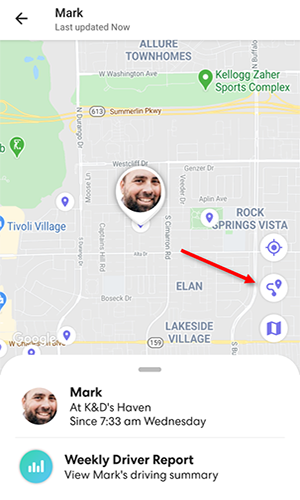
\includegraphics[width=0.45\textwidth]{Introduccion/life360-screenshot.png}
        \caption{Mapa de Life365}
        \label{fig:life365}
    \end{minipage}\hfill
    \begin{minipage}{0.45\textwidth}
        \centering
        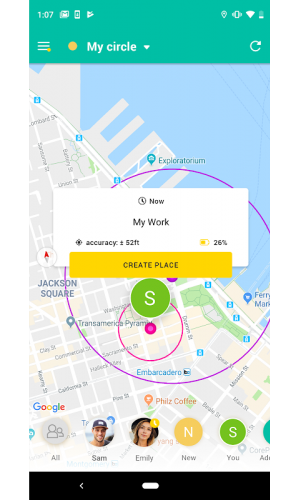
\includegraphics[width=0.45\textwidth]{Introduccion/geozilla-screenshot.png}
        \caption{Mapa de GeoZilla}
        \label{fig:geozilla}
    \end{minipage}
\end{figure}
\vspace{-20pt}
Aún con todo, estas aplicaciones transversales tienen el inconveniente de la carencia del enfoque en la enfermedad. Los gestores de tareas grupales tienden a tener un enfoque profesional para la gestión de equipos de trabajo y con ello tienen un alcance excesivo para el tipo de recordatorios que se deben manejar, complicando su uso para estos menesteres. Las aplicaciones de geolocalización, por otro lado, aunque no están centradas en esta misma enfermedad, sí están diseñadas con necesidades similares en mente y por ello ofrecen una experiencia óptima para el uso que se daría en este ámbito. Lo mismo se puede decir de las aplicaciones de mensajería, que con su diseño generalista también son idóneas para utilizar en los casos que nos ocupan.

Respecto a estos conjuntos de aplicaciones más dedicadas, el aporte que pretende ofrecer \emph{All for One} radica en la comunión de todas estas funcionalidades en un único sistema, evitando configuraciones extra o varias instalaciones para poder contar con todas. Permitiendo a su vez, facilidad en el uso interrelacionado de estas funcionalidades sin excesivos pasos extra y con un canal único de notificaciones común.

\subsection{Evaluación de alternativas}

Dejando a un lado las aplicaciones que ofrecen coincidencias parciales o moderadas podemos pasar a un estudio enfocado en la evaluación de las aplicación con mayores coincidencias y con similutes más directas. Se han seleccionado tres de estas aplicaciones para ofrecer una revisión más dedicada de la que extraer conclusiones que aporten a la hora de diseñar y desarrollar \textbf{All for One}.

\subsubsection{Trusted Elderly Care}

\begin{wrapfigure}[6]{r}{0.2\textwidth}
    \vspace{-20pt}
    \centering
    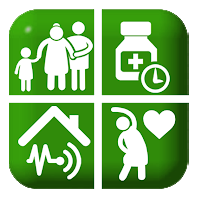
\includegraphics[width=0.15\textwidth]{images/Introduccion/elderly-icon.png}
    \vspace{-17pt}
    \caption{Icono de Elderly Care}
\end{wrapfigure}

Trusted Elderly Care es una aplicación desarrollada por \textbf{LEVStone} disponible en la PlayStore\footnote{\href{https://play.google.com/store/apps/details?id=com.levstone.mobility.trustedelderlycare}{https://play.google.com/store/apps/details?id=com.levstone.mobility.trustedelderlycare}} de Android. La aplicación está enfocada en la monitorización de familiares, especialmente ancianos, y aunque se ofrece de forma gratuita necesita un pago de seis euros para crear los grupos que se usan para el monitoreo, sin embargo, una única cuenta que lo haya adquirido ya permite crear un grupo para todos los familiares. Además de eso, la compañía acepta donaciones en su página web\footnote{\href{https://levstone.com/health-family/trusted-elderly-care/}{https://levstone.com/health-family/trusted-elderly-care/}}.

Como se ha dicho, la aplicación gira en torno a la \textbf{creación de grupos} a los que se deben unir los usuarios para obtener información del resto de usuarios. Entre las funciones que ofrece la aplicación están: elegir un emoji que represente el estado de ánimo, sincronizar la aplicación con sensores y obtener sus lecturas, consultar un mapa con las localizaciones de los usuarios, activar un modo pánico, acceder a los contactos del grupo o crear y consultar tareas entre otras cosas.

La mayoría de estas acciones y otros sucesos relacionados con el usuario como el nivel de carga o el último momento de uso del teléfono móvil \textbf{son notificados al resto de usuarios} del grupo. Sin embargo, el sistema de notificaciones no es instantáneo, la aplicación se debe refrescar para obtener los nuevos cambios en las pantallas o las notificaciones. La aplicación se refresca según el tiempo que el usuario establece en ajustes o usando manualmente el botón de refresco.

\begin{figure}[h]
    \centering
    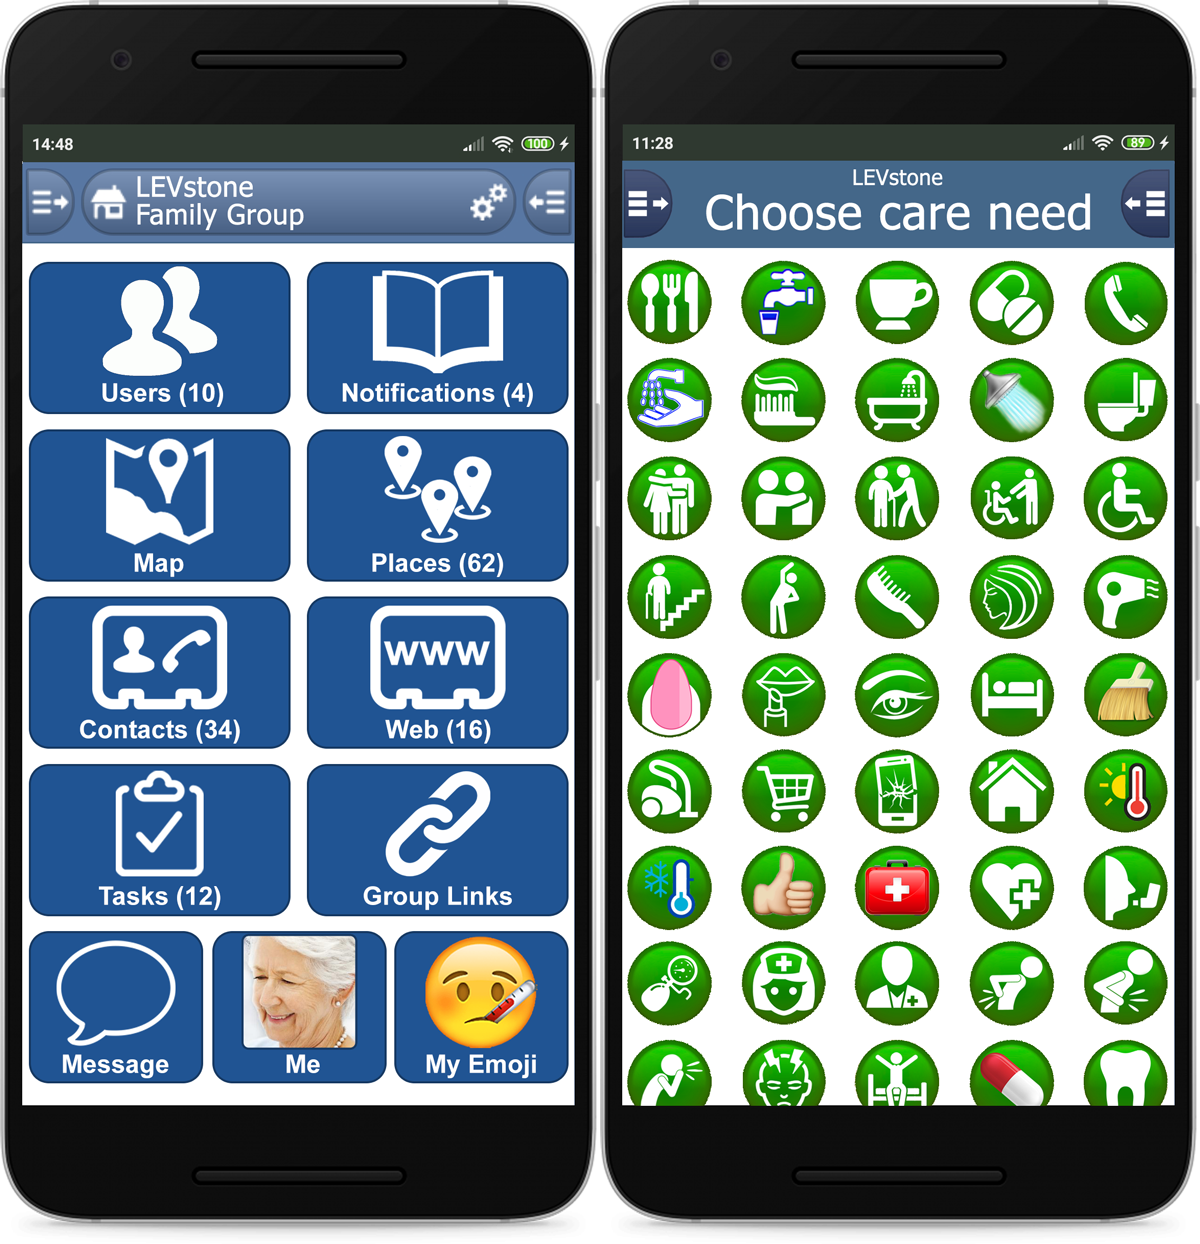
\includegraphics[width=0.5\textwidth]{images/Introduccion/elderly-screenshot.png}
    \caption{Capturas de pantalla de la página web Elderly Care}
\end{figure}

La aplicación permite personalización en bastantes apartados y amplio nivel de detalle y opciones en el uso de sus herramientas. Las tareas que permite crear cuentan con un amplia variedad de campos como establecer la hora y lugar de comienzo y final, el tipo de tarea o los usuarios relacionados con la misma, así como la opción de añadir imágenes o enlaces. En la función de localización ofrece la opción de guardar localizaciones que luego pueden servir, además de para mostrarlas en el mapa, para crear avisos rápidos de estar dirigiéndose hacia el lugar o para ponerlo como lugar donde se llevará a cabo una tarea.

\textbf{El uso de la aplicación es difícil}. La interfaz es ofuscada, está llena de información y no la presenta con iconos o convenciones habituales. Entre otras cosas, los filtros de la ventana de notificaciones están en diferentes botones, nombrados como Usuario o Lugar, que no ofrecen ninguna información de su utilidad. Sin embargo, el mayor problema radica en la navegación, es abstracta y enrevesada, dificultando el acceso al gran número de funciones. Esto es un gran problema de cara a una aplicación pensada para ser usada por gente de avanzada edad, que tienen menos manejo con las tecnologías además de peor visión o memoria entre otras cosas.

\textbf{Virtudes}
\begin{itemize}
    \item Herramienta de tareas muy completa e informativa.
    \item La capacidad de guardar lugares en el mapa.
    \item La vinculación de sensores biométricos.
\end{itemize}

\textbf{Inconvenientes}
\begin{itemize}
    \item Elevado consumo de batería por el monitoreo de recursos.
    \item Navegación ofuscada y enrevesada.
    \item Necesidad de refresco manual para la recepción de nueva información.
    \item Interfaz sobrecargada y poco intuitiva.
\end{itemize}

\subsubsection{Tú y nosotros}

Tú y nosotros (o como aparece en la Play Store\footnote{\href{https://play.google.com/store/apps/details?id=com.tuynosotros.alzheimertyn}{https://play.google.com/store/apps/details?id=com.tuynosotros.alzheimertyn}}, \textbf{Alzheimer App TyN}) es una aplicación desarrollada por A. Calvo. Su principal función es almacenar una ficha con los datos del paciente de Alzheimer y de uno de sus cuidadores (\fref{fig:tyn-ficha}) para que el paciente siempre tenga esa información a mano. Su otra función principal es permitir la creación de recordatorios. Además, \textbf{tiene dos juegos} para el ejercicio mental y un botón para realizar llamadas de emergencia. Como muchas otras aplicaciones también contiene información y enlaces de interés.

Los recordatorios que se pueden crear están compuestos por un nombre que lo define y por una hora a la que se deba recordar. Cuando llega dicha hora \textbf{una notificación es enviada al usuario} con el aviso, de forma que favorece que la pueda llevar a cabo. Además de eso, la notificación se puede marcar como repetible, lo cual hará que esta se notifique diariamente. El usuario también tiene disponible una lista desde la que consultar y eliminar sus recordatorios guardados.

\begin{wrapfigure}[6]{r}{0.2\textwidth}
    \vspace{-20pt}
    \centering
    
\includegraphics[width=0.15\textwidth]{Introduccion/tyn-icon.png}
    \vspace{-10pt}
    \caption{Icono de Tú y Nosotros}
\end{wrapfigure}

Los juegos ofrecidos por la aplicación son: \textbf{Memoria} (\fref{fig:tyn-memoria}), un juego de parejas con un tablero 4x4 para recordar y juntar parejas de imágenes de conceptos comunes como utensilios, animales o vehículos; y \textbf{Reconoce}, juego en el que se sirven al jugador dos columnas, una con imágenes del mismo tipo que Memoria y otra con los nombres de estos, el jugador debe relacionar cada objeto o animal con el sustantivo que lo nombra.

La aplicación es sencilla de utilizar y muy clara. Sin embargo, \textbf{no cuenta con perfiles ni con interconexión} entre aplicaciones. Es una aplicación con ejecución y persistencia local que no permite la interacción entre cuidadores y pacientes, de hecho, es una aplicación destinada únicamente a los dispositivos de los clientes. Si un cuidador quisiese incluir su información o añadir recordatorios al paciente debería hacerlo desde el móvil del mismo.

\textbf{Virtudes}
\begin{itemize}
    \item Manejo muy sencillo y apto para cualquier usuario.
    \item Aviso por notificación de los recordatorios.
    \item Ficha con información útil para los pacientes.
\end{itemize}

\textbf{Inconvenientes}
\begin{itemize}
    \item No permite ayudar al paciente de forma remota.
    \item Los recordatorios permiten poca información u opciones.
    \item Visualmente le falta claridad en algunos apartados.
\end{itemize}

\vspace{25pt}

\begin{figure}[H]
    \centering
    \begin{minipage}{0.45\textwidth}
        \centering
        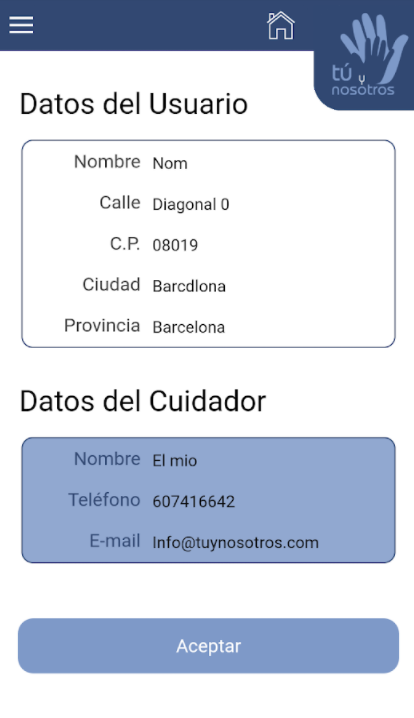
\includegraphics[width=0.45\textwidth]{Introduccion/tyn-screenshot-1.PNG}
        \caption{Ficha de contacto de Tú y Nosotros}
        \label{fig:tyn-ficha}
    \end{minipage}\hfill
    \begin{minipage}{0.45\textwidth}
        \centering
        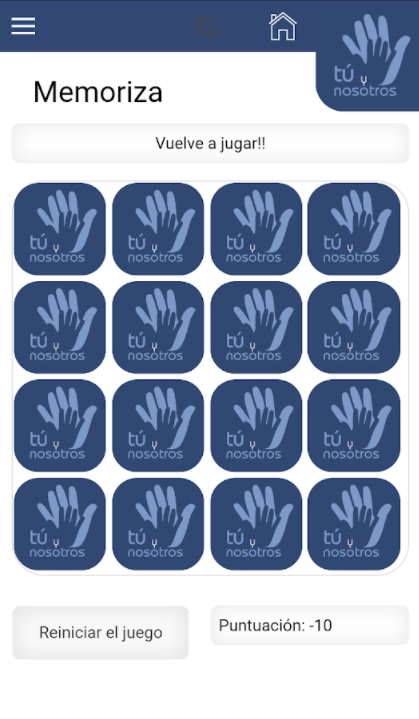
\includegraphics[width=0.45\textwidth]{Introduccion/tyn-screenshot-2.PNG}
        \caption{Juego de memoria de Tú y Nosotros}
        \label{fig:tyn-memoria}
    \end{minipage}
\end{figure}                  % REV?
\chapter{Aspectos teóricos}
\label{ch:aspectos_teoricos}

En este capítulo se presentarán una definición de una serie de conceptos de la especialidad que son clave en la comprensión del proyecto que nos aborda.

\section{API REST}

En el año 2000, Roy Fielding publicó \emph{Architectural Styles and the Design of Network-based Software Architectures}\cite{fielding2000architectural}, disertación en la que presentó al mundo la transferencia de estado representacional o \acrshort{rest}.

\acrshort{rest} es una propuesta de arquitectura para aplicaciones web basada en la comunicación de representaciones del estado en las peticiones siguiendo las especificaciones \acrshort{http}. En una petición \acrshort{rest} un cliente hace una petición al servidor con una serie de encabezados y parámetros que serán usados en el extremo solicitado para procesarla y responder a la petición con una representación del recurso solicitado y una nueva serie de encabezados con información acerca de la petición como el código de estado o el formato de la respuesta.

Por otro lado, una \acrshort{api} es una interfaz de programación de aplicaciones utilizada en la definición, diseño e integración de software para especificar los requisitos en las dos partes de la comunicación entre los sistemas software que la emplean para garantizar el éxito de la transferencia.

Una \acrshort{api} \acrshort{rest} es, por tanto, una serie de definiciones y protocolos que se adapta a la arquitectura \acrshort{rest}, permitiendo una interacción con la que los clientes puedan transferir y recibir recursos de un servidor por medio de peticiones \acrshort{http} sin estado, esto es que cada una es independiente de todas las demás. La comunicación entre un cliente y un servidor con una \acrshort{api} \acrshort{rest} se realiza por medio de extremos o \glspl{endpoint}.

Los recursos de una \acrshort{api} \acrshort{rest} deben, a su vez, seguir una interfaz de comunicación estándar que facilite la comunicación total con el servicio a la vez que permite el manejo y gestión del recurso a partir de la representación transferida en la comunicación.

\section{WebSocket}

El protocolo WebSocket es una interfaz de comunicación a través de un único canal \acrshort{tcp}. Este protocolo ofrece una comunicación en tiempo real a través de una \acrshort{api} que permite que los extremos de la comunicación (cliente y servidor) puedan enviarse mensajes sin una petición previa del receptor. WebSocket fue estandarizado en 2011 con el \emph{RFC 6455}\cite{rfc6455} por el \acrshort{ietf}.

La comunicación de los WebSocket se realiza a través de \Gls{uri} con un nuevo esquema que comienza por \code{ws:} o \code{wss:}, según sean para transmisiones no encriptadas o encriptadas respectivamente, equivalentes a las similares de \acrshort{http}. Dichos enlaces son utilizados para establecer un canal de comunicación, cerrarlo o para utilizarlo para enviar un mensaje.

Las \acrshort{api} de comunicación por medio de WebSocket lo aplican por medio de un patrón de suscripción, asignando a los identificadores de los diferentes tipos de mensaje un punto de escucha con una función o servicio a ejecutar cuando se reciba un nuevo mensaje. El envío de mensajes de un cliente a un servidor es elemental, pero la comunicación servidor-cliente puede ser única o de difusión, enviando el mismo mensaje a una serie de clientes conectados.

\section{NoSQL}

El término NoSQL (del inglés \emph{Not only \acrshort{sql}}) engloba una serie de tecnologías de bases de datos que se apartan del clásico modelo de gestión de bases de datos relacionales cuyo principal representante es \acrshort{sql}. Las características comunes son que permiten la consulta sin necesidad de emplear \acrshort{sql}, están diseñadas para favorecer la escalabilidad sacrificando la consistencia o atomicidad y apuestan por la flexibilidad.

Existen muchos tipos de sistemas de gestión NoSQL siendo los más resaltables:
\begin{enumerate}
	\item \textbf{Bases de datos documentales}, basadas en el almacenamiento de documentos asociados a una clave única. La gran fortaleza de estas bases de datos radica en la capacidad de guardar y recuperar grandes volúmenes de datos con facilidad y gran flexibilidad. Los documentos más habituales son de formato \acrshort{json} (conjunto de pares clave-valor, clave-matriz o clave-documento). Un ejemplo de este tipo de bases de datos es MongoDB\footnote{\href{https://www.mongodb.com/}{https://www.mongodb.com/}} (\fref{ssec:mongodb}).
	\item \textbf{Bases de datos de grafos}, enfocados en las relaciones entre entidades. Su mayor ventaja radica en la rápida navegación y agregación de datos que basan con sus relaciones, mucho más ágil que los \emph{\gls{join}} de \acrshort{sql}. La base de datos de grafos más popular es Neo4J\footnote{\href{https://neo4j.com/}{https://neo4j.com/}}.
	\item \textbf{Almacenes de clave-valor}. La bases de datos más atómicas. Almacenan pares de clave y valor sin mayor estructura o relación, lo que las hace muy veloces para la recuperación de información básica conocida y un complemento habitual de otras bases de datos para proporcionar una caché de acceso veloz a datos habitualmente solicitados. Redis\footnote{\href{https://redis.io/}{https://redis.io/}}, por ejemplo, es una base de datos clave-valor que funciona en memoria.
	\item \textbf{Bases de datos orientadas a columnas}. En las bases de datos \acrshort{sql} que almacenan los datos en filas, favoreciendo el acceso a las propiedades completas de una entidad. En una base de datos columnar, la disposición favorece el acceso a los conjunto de propiedades de las entidades, haciéndolas destacar en la evaluación de grandes volúmenes de datos, sacrificando rendimiento en las transacciones. Una base de datos de este estilo es Apache Cassandra\footnote{\href{https://cassandra.apache.org/}{https://cassandra.apache.org/}}. 
\end{enumerate}

Otros tipos de bases de datos NoSQL son, por ejemplo, las bases de datos orientadas a objetos o las bases de datos multivalor entre otras.

\part{Planificación}                                        
\chapter{Requisitos iniciales}
\label{ch:requisitos_iniciales}

En la planificación inicial del sistema se han definido unos primeros requisitos generales a considerar para usar como base en todo el tramo de planificación.

\begin{enumerate}[label*=RI\arabic*.]
    \item El sistema ofrecerá una aplicación móvil.
    \begin{enumerate}[label*=\arabic*.]
        \item La aplicación estará disponible en Android.
        \item La aplicación permitirá el inicio de sesión en la aplicación con una cuenta de Google.
        \item La aplicación permitirá cerrar la sesión.
        \item Los usuarios podrán cubrir su perfil con datos personales.
        \item Los usuarios recién creados podrán elegir un rol.
        \begin{enumerate}[label*=\arabic*.]
            \item Paciente.
            \item Cuidador.
        \end{enumerate}
        \item Los Pacientes y Cuidadores podrán vincularse.
        \begin{enumerate}[label*=\arabic*.]
            \item Un Paciente podrá tener varios Cuidadores.
            \item Un Cuidador podrá tener sólo un Paciente.
        \end{enumerate}
        \item Los Pacientes y Cuidadores podrán desvincularse.
        \item La aplicación ofrecerá una serie de herramientas a los usuarios registrados y vinculados.
        \begin{enumerate}[label*=\arabic*.]
            \item Los Pacientes podrán ver su ficha personal.
            \item Los Cuidadores podrán ver la ficha personal de su Paciente vinculado.
            \item Los Pacientes y sus Cuidadores podrán comunicarse en una sala de chat compartida.
            \item Los Pacientes y sus Cuidadores podrán gestionar tareas para el Paciente.
            \begin{enumerate}[label*=\arabic*.]
                \item Los Pacientes y sus Cuidadores podrán crear una nueva tarea.
                \item Los Pacientes y sus Cuidadores podrán consultar las tareas existentes.
                \item Los Pacientes y sus Cuidadores podrán marcar una tarea como hecha.
                \item Los Pacientes y sus Cuidadores podrán marcar una tarea como no hecha.
                \item Los Pacientes podrán eliminar cualquier tarea.
                \item Lo usuario de tipo Cuidador podrán eliminar las tareas que han creado ellos mismos.
            \end{enumerate}
            \item Los Pacientes y sus Cuidadores podrán compartir su ubicación.
            \item Los Pacientes y sus Cuidadores podrán consultar en un mapa la ubicación compartida por los demás usuarios relacionados.
            \item Los Pacientes y sus Cuidadores podrán consultar el listado de Cuidadores del paciente.
            \begin{enumerate}[label*=\arabic*.]
                \item Los Pacientes y sus Cuidadores podrán consultar los datos de los Cuidadores. 
            \end{enumerate}
            \item Los Pacientes y sus Cuidadores serán notificados de las acciones clave de los usuarios relacionados.
            \item Los Pacientes y sus Cuidadores podrán consultar sus notificaciones pendientes.
        \end{enumerate}
    \end{enumerate}
    \item El sistema contará con un servidor desplegado en la nube para manejar la lógica.
    \item El servidor del sistema ofrecerá una \acrshort{api} \acrshort{rest}.
    \begin{enumerate}[label*=\arabic*.]
        \item La \acrshort{api} ofrecerá \glspl{endpoint} para la gestión de sesión de usuarios. 
        \begin{enumerate}[label*=\arabic*.]
            \item La \acrshort{api} ofrecerá un \gls{endpoint} para tramitar el inicio de sesión. 
            \item La \acrshort{api} ofrecerá un \gls{endpoint} para refrescar la sesión.
            \item La \acrshort{api} ofrecerá un \gls{endpoint} para cerrar la sesión.
        \end{enumerate}
        \item La \acrshort{api} ofrecerá \glspl{endpoint} para la gestión de información de usuarios. 
        \begin{enumerate}[label*=\arabic*.]
            \item La \acrshort{api} ofrecerá un \gls{endpoint} para actualizar los datos de un usuario. 
            \item La \acrshort{api} ofrecerá un \gls{endpoint} para recuperar la información de un Paciente vinculado. 
            \item La \acrshort{api} ofrecerá un \gls{endpoint} para recuperar la información de los Cuidadores de un Paciente. 
        \end{enumerate}
        \item La \acrshort{api} ofrecerá \glspl{endpoint} para la gestión de los vínculos de usuarios. 
        \begin{enumerate}[label*=\arabic*.]
            \item La \acrshort{api} ofrecerá un \gls{endpoint} para crear un código de vinculación. 
            \item La \acrshort{api} ofrecerá un \gls{endpoint} para crear un vínculo entre un Paciente y un Cuidador.
            \item La \acrshort{api} ofrecerá un \gls{endpoint} para eliminar un vínculo entre un Paciente y un Cuidador.
        \end{enumerate}
        \item La \acrshort{api} ofrecerá \glspl{endpoint} para la gestión de tareas. 
        \begin{enumerate}[label*=\arabic*.]
            \item La \acrshort{api} ofrecerá un \gls{endpoint} para crear una tarea. 
            \item La \acrshort{api} ofrecerá un \gls{endpoint} para listar las tareas. 
            \item La \acrshort{api} ofrecerá un \gls{endpoint} para eliminar una tarea.
            \item La \acrshort{api} ofrecerá un \gls{endpoint} para marcar una tarea como completada.
            \item La \acrshort{api} ofrecerá un \gls{endpoint} para marcar una tarea como no completada.
        \end{enumerate}
        \item La \acrshort{api} ofrecerá \glspl{endpoint} para la gestión de mensajes. 
        \begin{enumerate}[label*=\arabic*.]
            \item La \acrshort{api} ofrecerá un \gls{endpoint} para recuperar los mensajes más recientes.
        \end{enumerate}
        \item La \acrshort{api} ofrecerá \glspl{endpoint} para la gestión de notificaciones. 
        \begin{enumerate}[label*=\arabic*.]
            \item La \acrshort{api} ofrecerá un \gls{endpoint} para recuperar las notificaciones no leídas.
            \item La \acrshort{api} ofrecerá un \gls{endpoint} para marcar una notificación como leída.
            \item La \acrshort{api} ofrecerá un \gls{endpoint} para marcar todas las notificaciones como leídas.
        \end{enumerate}
    \end{enumerate}
    \item El servidor del sistema ofrecerá un servicio de WebSocket para comunicación con la aplicación.
    \begin{enumerate}[label*=\arabic*.]
        \item El sistema permitirá establecer la conexión desde la aplicación.
        \item El sistema gestionará las desconexiones.
        \item El sistema gestionará eventos de una sala global.
        \begin{enumerate}[label*=\arabic*.]
            \item El sistema escuchará un evento de subscripción a la sala global.
        \end{enumerate}
        \item El sistema gestionará eventos de una sala de localización.
        \begin{enumerate}[label*=\arabic*.]
            \item El sistema escuchará un evento de subscripción a la sala de localización.
            \item El sistema escuchará un evento de actualización de localización.
            \item El sistema escuchará un evento de desconexión a la sala de localización.
        \end{enumerate}
        \item El sistema gestionará eventos de una sala de mensajería.
        \begin{enumerate}[label*=\arabic*.]
            \item El sistema escuchará un evento de subscripción a la sala de mensajería.
            \item El sistema escuchará un evento de envío de mensajes.
            \item El sistema escuchará un evento de desconexión a la sala de mensajería.
        \end{enumerate}
        \item El sistema gestionará eventos de una sala de notificaciones.
        \begin{enumerate}[label*=\arabic*.]
            \item El sistema escuchará un evento de subscripción a la sala de notificaciones.
            \item El sistema escuchará un evento de comunicación de notificaciones.
            \item El sistema escuchará un evento de desconexión a la sala de notificaciones.
        \end{enumerate}
    \end{enumerate}
\end{enumerate}
\chapter{Evaluación de alternativas}
\label{ch:evaluacion_alternativas}

\section{Desarrollo de la aplicación móvil en Android}

\subsection{Desarrollo nativo en Java}

Java es el lenguaje principal utilizado a lo largo de todo el grado y en base a lo mismo también el lenguaje con el que el equipo de desarrollo cuenta con \textbf{más experiencia y soltura}. Es a su vez el primer lenguaje que fue seleccionado por Google para el desarrollo nativo en Android.

Esta opción ha sido largamente considerada puesto que, además, conforma el punto de conocimiento del equipo acerca del desarrollo de aplicaciones móviles por la asignatura\footnote{SDM: Software para Dispositivos Móviles} del grado centrada en esto. A pesar de esto, la siguiente alternativa, Kotlin, ofrece todas las capacidades de Java más algunos añadidos y mejoras que se han considerado suficientes para \textbf{desechar esta opción} respecto a la siguiente.

\subsection{Desarrollo nativo en Kotlin}

Kotlin es un lenguaje, desarrollado por \textbf{JetBrains} en 2011, de tipado estático que funciona sobre la \acrlong{jvm} y cuya filosofía de creación es la mejora y extensión de Java manteniendo toda una interoperabilidad total con código Java. En el año 2017 fue nombrado por Google como \textbf{lenguaje oficial de Android}\cite{kotlin2017}, y en 2019 lo declararon como el lenguaje preferido para dicho sistema operativo\cite{kotlin2019}, sustituyendo a Java.

Los desarrolladores de Kotlin son los mismos que están detrás del \textbf{Android Studio}, el \acrshort{ide} por antonomasia para el desarrollo en Android, y esto permite que dicho entorno facilite en gran medida el paso de Java a Kotlin con auto-conversión de código entre otras cosas. Esta facilidad, más la oficialidad de Kotlin como lenguaje por excelencia de Android y el interés por parte del equipo de desarrollo de aprender nuevas herramientas en auge han auspiciado \textbf{la selección de esta alternativa} para construír la aplicación.

\subsection{Desarrollo con el framework React Native}

La otra opción que se barajó para el desarrollo de la aplicación fue la opción de utilizar algún \textbf{framework multiplataforma} que permitiese también el desarrollo de la aplicación para iOS o que, al menos, ofreciese otro lenguaje o sistema para el desarrollo. Uno de los frameworks más extendidos de este tipo es \textbf{React Native}.

React Native permite el desarrollo de la aplicación utilizando Javascript y React\footnote{Librería de Javascript para el desarrollo de interfaces de usuario desarrollada por FAcebook}, que luego es compilado a código nativo de Android. El equipo de desarrollo cuenta con cierta experiencia en el uso del mismo, en base a la cual también se sabe que el uso de dichos frameworks no es óptima y provoca muchos problemas derivados de trabajar con ellos. Puesto que iOs no es un requisito para la aplicación (e inviable para el equipo de desarrollo por carencia de dispositivos) se ha \textbf{descartado esta opción}.

\section{Desarrollo de la API}

\subsection{Spring Framework}

Spring es un framework de código abierto para el desarrollo de aplicaciones ejecutables sobre la \acrshort{jvm}, admitiendo desarrollo en \textbf{Java y Kotlin}. A día de hoy es la plataforma base de la mayoría de aplicaciones empresariales desarrolladas en Java. Ofrece herramientas de sencilla ejecución como el despliegue sobre un servidor Apache o inyección de dependencias facilitando el desarrollo. Por defecto, usa JUnit como librería de pruebas.

Es una de las dos tecnologías con las que se ha aprendido a desarrollar aplicaciones web con controladores \acrshort{api} \acrshort{rest} en el grado\footnote{En la asignatura de Sistemas Distribuidos e Internet (SDI)}, por lo que el equipo de desarrollo cuenta con experiencia en su uso. Aún con todo, y a pesar de admitir el desarrollo en el mismo lenguaje en que se desarrollará la aplicación móvil se ha decidido \textbf{descartar esta opción} pues las tecnologías y herramientas que ofrece para el desarrollo con WebSockets es más complicada que las librerías ofrecidas por otras alternativas.

\subsection{Node.js con Express y Socket.io}

Node.js es un entorno multiplataforma para el desarrollo de servidores y aplicaciones basado en el \textbf{Javascript}, aunque acepta otros lenguajes compilables a Javascript como \textbf{Typescript}. El desarrollo en Node está basado en un amplio entorno de librerías. La librería más extendida para la creación de \acrshort{api} \acrshort{rest}s es \textbf{Express}, que será la considerada en esta alternativa. Para el trabajo con WebSockets se considerará \textbf{Socket.io} y para las pruebas se elegirá \textbf{Jest}, ambas son librerías conocidas por la facilidad de uso.

Node es la otra tecnología con la que se ha aprendido a trabajar en el grado\footnote{También en la asignatura de Sistemas Distribuidos e Internet (SDI)}, por lo que, de nuevo, el equipo de desarrollo cuenta con experiencia en este campo. Debido a la agilidad que ofrece y la sencillez de manejo de la librería de WebSockets (así como el que esta cuenta con una librería para implementar el cliente en Android) se \textbf{ha estimado elegir esta alternativa}. La \acrshort{api} se desarrollará en Node.js utilizando Typescript y con Express, Socket.io y Jest como librerías de enrutamiento \acrshort{rest}, de WebSocket y de testing respectivamente.

\subsection{Micronaut}

Micronaut es también un framework open-source para el desarrollo de aplicaciones sobre la \acrshort{jvm} que admite desarrollo en \textbf{Java, Groovy y Kotlin}. Micronaut ofrece una revisión sobre frameworks más antiguos como Spring haciendo énfasis en un diseño orientado a la nube u optimizaciones varias, por ejemplo, haciendo la inyección de dependencias con funcionamiento bajo demanda para reducir el peso y el tiempo de despliegue o testing (basado también en JUnit).

Una de las ventajas de Micronaut, su modernidad, es también uno de sus mayores defectos pues carece de la amplia documentación o ejemplos que sí tenían las otras dos alternativas gracias a su longevidad y amplio uso. Es por este motivo por el que el equipo de desarrollo, aún teniendo cierta experiencia con el mismo, ha decidido \textbf{descartar Micronaut} para reducir en lo posible los bloqueos derivados del uso del framework.

\section{Tecnología de geolocalización}

\subsection{OsmDroid}

\textbf{OpenStreetMap} es un proyecto colaborativo de mapeado global y de software libre que construye sus mapeados gracias a la aportación de los dispositivos \acrshort{gps} y a los añadidos manuales de sus contribuyentes. OpenStreetMap ofrece una \acrshort{api} gratuita para la consulta y acceso a los datos albergados y a su mapa digital.

La librería más completa para trabajar con OpenStreetMap en Android es \textbf{OsmDroid}, que logra un reemplazamiento casi completo de la primera versión de la \acrshort{api} de mapas de Android con su código abierto. Sin embargo, esta librería aún no tiene el pulido de sus hermanas web y cuenta con menos documentación o ejemplos que la librería oficial de Google. Por lo que \textbf{no se considera} su uso contra esta. 

\subsection{Google Maps for Android}

Google Maps es la \acrshort{api} más extendida y usada del mundo para la implementación de mapas, sistemas de geolocalización o de navegación, entre otras cosas. Su precio varía según la plataforma donde se use y según las herramientas del mismo o el número de llamadas que se hagan a la API. Sin embargo, en el momento del desarrollo del proyecto \textbf{es gratuita para las aplicaciones de Android} con sus servicios básicos.

El único servicio que está planeado para la aplicación es el de la visualización del mapa en las coordenadas especificadas y este se encuentra incluido en el paquete gratuito. Además, la empresa desarrolladora de Android y de la \acrshort{api} son la misma y de ello deriva que la librería que la emplea sea la más completa y funcional del sistema operativo. Por estas razones se decidió \textbf{optar por estar alternativa}.

\section{Sistema de gestión de bases de datos}

De cara a la selección de un sistema de gestión de bases de datos, debido al tipo de información que se manejarán en los chats, se seleccionó una \textbf{base de datos documental} como la mejor opción para el desarrollo de esta aplicación, dos gestores de este tipo fueron considerados:

\subsection{MongoDB}
\label{ssec:mongodb}

MongoDB es la base de datos por excelencia en el mundo de las bases de datos documentales e incluso lidera ampliamente el conjunto de todos los sistemas de bases de datos NoSQL\cite{dbEnginesRanking}. MongoDB es un proyecto de código abierto y es compatible tanto con la nube privada, mediante el despliegue de la base de datos en los servidores del sistema que la vaya a utilizar; como con la nube pública, por medio del servicio \textbf{MongoDB Atlas}.

MongoDB Atlas ofrece niveles del servicio gratuitos y, además, un crédito de 500\$ para estudiantes. Los requisitos iniciales del sistema son compatibles con los rangos que permiten estas dos opciones, sumado a su extendido uso, a la experiencia del equipo de desarrollo y facilidad de implementación en Node.js, se ha \textbf{elegido esta alternativa}.

\subsection{Firebase}

Firebase es una plataforma para el desarrollo móvil y web de Google que ofrece una serie de herramientas como un sistema de autenticación o una base de datos documental entre otras cosas. Está ampliamente documentada e implementada en gran número de aplicaciones Android.

Su sistema de gestión de bases de datos es documental en formato \acrshort{json} y se llama \textbf{Realtime Database}. Sin embargo, y a pesar de que su coste sería gratuito para los propósitos iniciales de \emph{All for One}, la serie de pasos que requiere para su uso en el sistema son un punto negativo respecto a la otra alternativa considerada y en base a esto, \textbf{no será la opción empleada}.

\section{Nube para el despliegue del servidor}

\subsection{Amazon Web Services}

Amazon Web Services (o AWS) es el servicio líder en cloud en el mundo\cite{cloud2021}. Derivado de esto se extiende una gran cantidad de documentación acerca de su uso y un servicio que se puede prever fiable. Además, el equipo de desarrollo ya ha desplegado anteriormente aplicaciones en este servicio. Lamentablemente, su coste es un problema para este desarrollo carente de inversión, por lo que se \textbf{ha decidido buscar otras alternativas}.

\subsection{Microsoft Azure}

Tras AWS, Azure de Microsoft es el siguiente servicio con mayor cuota de mercado\cite{cloud2021}, esto se traduce en unas virtudes similares a los nombrados en el punto anterior. Aunque el equipo de desarrollo no ha llevado a cabo ningún despliegue anterior sí ha acudido a un curso de formación\footnote{\textbf{Fundamentos de Microsoft Azure}, impartido por la Universidad de Oviedo en julio de 2021} relacionado con el mismo, por lo que tiene un conocimiento mucho mayor que con cualquier otro proveedor. Además, los estudiantes pueden recibir un crédito de 100\$ que puede ser suficiente para el despliegue necesario en este proyecto. La suma de todo esto ha convertido a Azure \textbf{en la opción elegida}.

\subsection{Heroku}

Puesto que el coste económico es el factor determinante en la decisión del proveedor de una nube para el despliegue del servidor, también se tuvo en amplia consideración otra alternativa, a pesar de carecer de total experiencia con ella. Heroku carece del mercado de las dos otras alternativas, pero ofrece un servicio de hosting para aplicaciones gratuito que habría sido suficiente para este proyecto. Aún con este punto positivo se decidió \textbf{optar por otra alternativa} más popular actualmente y que ofreciese un aprendizaje más útil de cara a la futura e inminente carrera profesional.       
\chapter{Análisis de riesgos}
\label{ch:analisis_riesgos}

A continuación se presentan los cuatro riesgos del proyecto detectados por el equipo de desarrollo. La descripción, análisis y respuesta al riesgo se han realizado siguiendo las indicaciones del PMBOK\cite{pmbok2013}.

\section{Descripción de riesgos detectados}

\subsection{Incapacidad de obtención de colaboración con asociaciones}

\begin{itemize}
    \item \textbf{Identificador}: Rsk-1
    \item \textbf{Categoría}: Externo
    \item \textbf{Subcategoría}: Subcontratistas y proveedores
\end{itemize}

Este riesgo parte de experiencia previa al comienzo del proyecto, basada en contactos preliminares que se intentaron antes de proponer la idea del mismo. 

El posible riesgo radicaría en no poder contar con el apoyo o colaboración de alguna asociación de pacientes de Alzheimer que pudiese aportar una opinión experta o consejos de utilidad para el diseño de la aplicación. Es un riesgo concretamente por la \textbf{falta de formación específica} en este área del equipo de desarrollo, algo que podría perjudicar la calidad del producto entregado.

Además, la alianza con una asociación de este estilo podría ser necesaria de cara a la realización de pruebas de usabilidad del sistema generado con usuarios objetivo. En caso de no obtenerla el proyecto tendría que ser entregado \textbf{sin una prueba de campo adecuada} a los objetivos y pretensiones iniciales.


\vspace{20pt}
\subsection{Inexperiencia del equipo de proyecto}

\begin{itemize}
    \item \textbf{Identificador}: Rsk-2
    \item \textbf{Categoría}: Dirección de Proyectos
    \item \textbf{Subcategoría}: Estimación y Planificación
\end{itemize}

Actualmente, la única experiencia del equipo de proyecto en la dirección y gestión de proyectos es el de la simulación realizada en la asignatura de DPPI\footnote{Dirección y Planificación de Proyectos Informáticos}. No existe una \textbf{experiencia práctica real} y esto puede manifestarse en forma de cálculos erróneos en la planificación del proyecto.

El riesgo radica en la posibilidad de aparición de estos errores. Como podrían ser, por ejemplo, \textbf{malas estimaciones} del tiempo necesario para completar tareas. Las desviaciones de esto desembocarían en grandes problemas de la planificación y también afectaría, en cascada, al cálculo del presupuesto o al alcance y calidad conseguibles por el sistema.

\subsection{Carencia de fondos}

\begin{itemize}
    \item \textbf{Identificador}: Rsk-3
    \item \textbf{Categoría}: Organizativo
    \item \textbf{Subcategoría}: Financiación
\end{itemize}

El riesgo en sí mismo no es la carencia de fondos, puesto que eso ya es un una característica conocida y definida de este proyecto. Sin embargo, sigue existiendo el riesgo de que dicha carencia de fondos sea problemática de cara a la consecución de la calidad deseada en el proyecto. La imposibilidad de costearse un servicio de alojamiento o de pagar ciertas \acrshort{api} o servicios de pago pueden suponer \textbf{complicaciones no previstas} para el proyecto inicialmente.

\subsection{Falta de formación en tecnologías clave}

\begin{itemize}
    \item \textbf{Identificador}: Rsk-4
    \item \textbf{Categoría}: Técnico
    \item \textbf{Subcategoría}: Tecnología
\end{itemize}

En el desarrollo se utilizarán varias tecnologías con las que no se cuenta con experiencia de desarrollo previo. Algunas de estas \textbf{son clave} para el funcionamiento del sistema. Este hecho supone un riesgo al poder provocar impedimentos o retrasos en la generación de los componentes que trabajen con dichas tecnologías. Así como en errores de funcionamiento o concepto derivados del desconocimiento de las capacidades completas de las tecnologías a manejar.

\section{Análisis de los riesgos}

\begin{table}[H]
    \centering
    \makebox[\textwidth]{
    \begin{tabular}{|l|c|c c c c|c|}
        \hline
        & & \multicolumn{4}{c|}{Impacto} & \\
        Riesgo & Probabilidad & Presupuesto & Planificación & Alcance & Calidad & Impacto \\
        \hline
        Colaboración con asociaciones & Alta  & Mínima  & Medio   & Alto  & Alta    & 0.39 \\
        Inexperiencia del equipo      & Media & Alto    & Crítico & Medio & Bajo    & 0.45 \\
        Carencia de fondos            & Media & Crítico & Bajo    & Medio & Medio   & 0.45 \\
        Formación en tecnologías      & Media & Bajo    & Alto    & Bajo  & Alto    & 0.28 \\
        \hline
    \end{tabular}}
    \caption{Probabilidades y impacto de los riesgos}
    \label{tab:riesgos}
\end{table}

\vspace{-20pt}
En base a este análisis del impacto global de los riesgos detectados se ha resaltado la inexperiencia del equipo de proyecto y la carencia de fondos como los riesgos de \textbf{mayor prioridad} a paliar, pues son aquellos que pueden afectar en mayor medida al éxito del proyecto.

\vspace{-20pt}
\section{Respuesta a los riesgos}

\vspace{-5pt}
Para los distintos riesgos detectados se han propuesto las siguientes respuestas:

\vspace{-5pt}
\begin{itemize}
    \item \textbf{Inexperiencia del equipo de proyecto}. Puesto que no existe la posibilidad de contratar una opinión más formada ni de adquirir la experiencia necesaria para paliar los posibles errores. Se ha decidido \textbf{mitigar} el riesgo. Se tendrá en cuenta desde el principio la posibilidad de fallar en el desarrollo de la planificación. Se tomarán medidas cautelares al respecto como dejar margen de tiempo prudencial antes de la fecha límite o guardar tiempo de vacaciones por si es necesario una dedicación extra para compensar los errores.
    \item \textbf{Carencia de fondos}. En respuesta a este riesgo se ha decidido buscar la mayor \textbf{mitigación} posible por medio de la aceptación del uso de tecnologías de pago cuando sea necesario y existan de beneficios de estudiante que los puedan costear.
    \item \textbf{Incapacidad de obtención de colaboración con asociaciones}. Ante la situación actual con la pandemia y la imposibilidad de retrasar el desarrollo en esperas o aras de conseguir la ansiada colaboración se ha decidido \textbf{asumir} la posibilidad de no lograr dicho apoyo.
    \item \textbf{Falta de formación en tecnologías clave}. Para afrontar este problema se ha decidido intentar \textbf{eliminar} el riesgo por medio de llevar a cabo formación específica en las tecnologías que se consideren oportunas. La idea es adquirir suficiente bagaje antes de comenzar el desarrrollo para reducir al mínimo los riesgos de la inexperiencia del equipo desarrollador.
\end{itemize}              
\chapter{Descripción de la solución propuesta}
\label{ch:solucion_propuesta}

\section{Aplicación móvil}

La aplicación móvil a desarrollar será una aplicación nativa de Android desarrollada con la última versión de Kotlin estable al momento de comienzo del desarrollo, \textbf{Kotlin 1.5.0}. El código Kotlin será compilado con la \acrshort{jvm} 1.8 como destino. El \acrshort{sdk} de Android objetivo de la aplicación será el SDK 31, kit de desarrollo de la versión más reciente del sistema operativo, Android 12. Sin embargo, el SDK mínimo soportado será el de \textbf{Android 8.1 Oreo} (SDK 26), este abanico equivale a ofrecer un sistema compatible con más del 80\% de dispositivos Android actualmente en el mercado\cite{statcounter2021android}.

\begin{figure}[H]
    \centering
    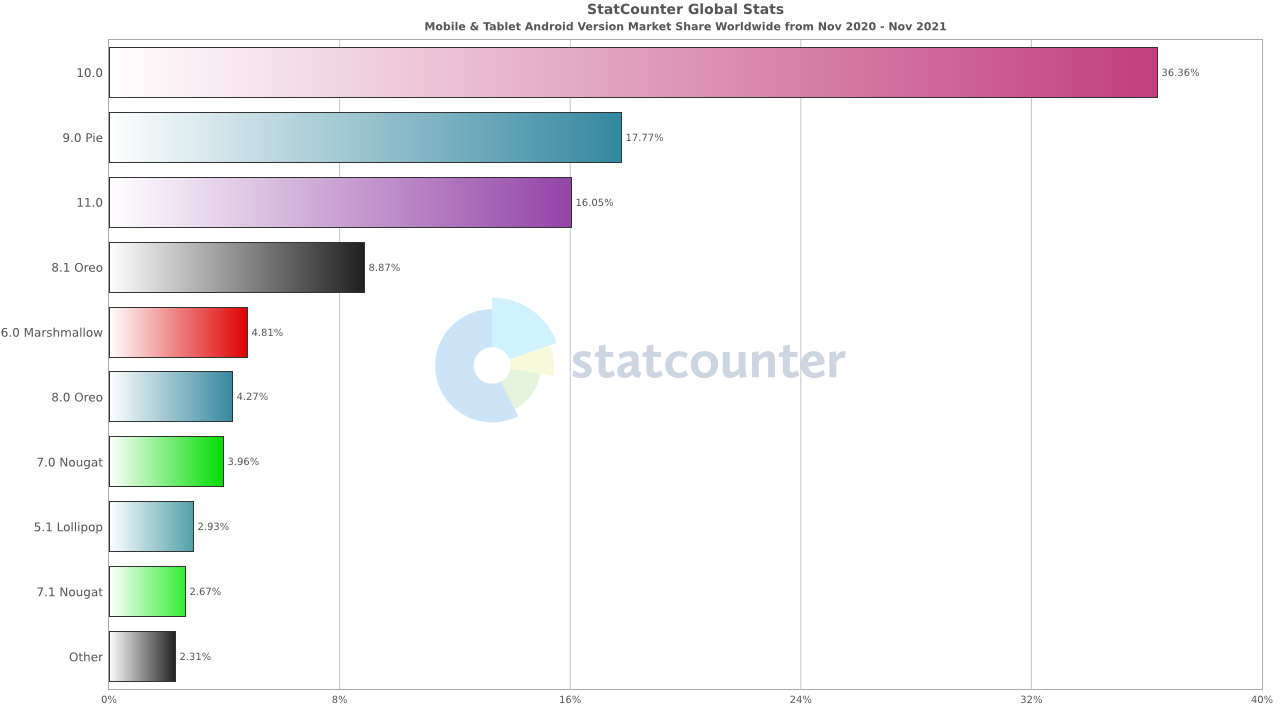
\includegraphics[width=1\textwidth]{images/Introduccion/android-stat.png}
    \caption{Reparto de mercado de Android (nov 20 - nov 21)}
    \label{fig:android-stats}
\end{figure}

Dicho desarrollo se realizará utilizando como herramienta principal el \acrshort{ide} Android Studio. La arquitectura de la aplicación será una \textbf{arquitectura \acrshort{mvvm}}, modelo de arquitectura recomendado actualmente para el desarrollo de aplicaciones Android\cite{mvvm2021}.
Las vistas se realizarán siguiendo las recomendaciones de \textbf{Material Design} (\fref{ssec:guia_material_design}). Las pruebas del sistema se llevarán a cabo con \textbf{JUnit 4} para las pruebas unitarias de componentes y con \textbf{Espresso} para las pruebas de comportamiento de las vistas. 

\subsection{Autenticación}

La autenticación de los usuarios en la aplicación se llevará a cabo siguiendo el protocolo \textbf{OAuth 2.0}\cite{rfc6749}. Dicha autenticación será lograda con apoyo en la \acrshort{api} de autenticación de Google, de esta forma el usuario podrá iniciar sesión con la cuenta Google que ya tiene vinculada al dispositivo o cualquier otra que desee usar. En una primera versión del sistema no se valora añadir otros métodos o vías de autenticación.

\subsection{Geolocalización}

Para la función de geolocalización se hará uso de los dispositivos \acrshort{gps} montados en los terminales de los usuarios. La obtención de la localización y su muestra en un mapa se llevarán a cabo con la \textbf{el kit de desarrollo de mapas de Google} (\ref{lib:app:maps}) para Android. La localización del usuario se comunicará al servidor por vía del WebSocket cuando comience a compartirla, por la misma vía se obtendrá también la localización del resto de usuarios vinculados.

\subsection{Comunicación con la API}

La comunicación por red con la \acrshort{api} se llevará a cabo haciendo uso de la librería \textbf{Retrofit 2} (\fref{lib:app:retrofit2}) de Square Open Source para la realización de peticiones \acrshort{rest}. La comunicación por medio de los WebSockets se llevará a cabo con el \textbf{cliente para Android de Socket.io} (\fref{lib:app:socketio}). El intercambio de datos en ambos protocolos hará uso de Gson\footnote{\href{https://github.com/google/gson}{https://github.com/google/gson}}, la librería de Google para la conversión de objetos Java a \acrshort{json} y viceversa. En los tests la simulación de la comunicación de la \acrshort{api} se realizará con el MockWebServer (\fref{lib:app:mockwebserver}) de Square Open Source.

\subsection{Vinculación de usuarios}

Para la realización de una vinculación de usuarios fiable a la vez que cómoda se realizará por medio del escaneo de códigos QR. Para gestionar la creación y escaneo de los mismos se utilizará \textbf{Zxing}\footnote{\href{https://github.com/zxing/zxing}{https://github.com/zxing/zxing}}, librería de Google para la codificación y decodificación de códigos de barras, códigos QR y similares.

\section{API}

El servidor con la \acrshort{api} y la lógica de negocio del sistema será desarrollada utilizando la última versión estable de Node.js, \textbf{Node v16}\footnote{\href{https://nodejs.org/en/about/releases}{https://nodejs.org/en/about/releases}}. Para fomentar la creación de código más mantenible y resistente a errores se usará como lenguaje de programación \textbf{Typescript} (\fref{lib:typescript}). El código Typescript será compilado a EcmaScript 6\cite{ecma262} con el módulo CommonJS. Para las pruebas se usará la librería \textbf{Jest} (\fref{lib:api:jest}), compatibilizada con Typescript por medio de TSJest (\fref{lib:api:ts_jest}).

El enrutamiento y el manejo de las peticiones \acrshort{http} de la \acrshort{api} \acrshort{rest} será desarrollado y gestionado con la librería \textbf{Express} (\fref{lib:api:express}). Sus pruebas serán manejadas con la librería SuperTest (\fref{lib:api:supertest}). Por otro lado, los WebSockets serán manejados por \textbf{Socket.io} (\fref{lib:api:socket_io}).

\subsection{Autenticación}

La autenticación en el servidor para el uso de la \acrshort{api} \acrshort{rest} será implementado por medio de Bearer tokens\cite{rfc6750}. Se manejarán dos tipos de token. El inicio de sesión se llevará a cabo por medio de \textbf{tokens de autenticación de Google} servidos por la app y que se verificarán por medio de Google Auth Library (\fref{lib:api:google_auth_library}). Una vez iniciada la sesión se proporcionarán tokens de autenticación y refresco para la realización de peticiones privadas a la \acrshort{api} \acrshort{rest}, estos tokens serán \textbf{\acrlong{jwt}}\cite{rfc7519}. La librería de \acrshort{npm}\footnote{Gestor de paquetes de Node.js} de \acrshort{jwt} será la que se usará para la creación, validación y verificación de estos tokens.

\subsection{Persistencia de datos}

La persistencia de datos se realizará con una base de datos documental de MongoDB alojada en la nube en remoto de \textbf{MongoDB Atlas}\footnote{https://www.mongodb.com/atlas/database}. Para el manejo de la base de datos se usará la librería Mongoose (\fref{lib:api:mongoose}). Para utilizarla con todas las fortalezas de Typescript se usará la librería \textbf{Typegoose} (\fref{lib:api:typegoose}). De cara a la ejecución de tests con persistencia se usará la librería de MongoDB Memory Server (\fref{lib:api:inmemory_server}) para replicar la base de datos en memoria.

\section{Despliegue}

La \acrshort{api} del sistema será desplegada en la nube haciendo uso del servicio \textbf{Microsoft Azure}. Puesto que los requisitos de uso del sistema en este proyecto serán mínimos se usará una \textbf{AppService de nivel B1} financiada por el crédito para estudiantes. Para el manejo del despliegue se creará una pipeline de despliegue continuo con GitHub Actions (\fref{tool:github_actions}) que actualice el sistema desplegado cuando se actualice el código de la rama principal del sistema. 
\chapter{Planificación temporal}
\label{ch:planificacion_temporal}

De cara a la realización de una planificación temporal se ha determinado un calendario de trabajo para el equipo de desarrollo implicado, en el proyecto que nos ocupa este equipo cuenta únicamente con un desarrollador. El desarrollador estará empleado en un trabajo ajeno al proyecto a jornada completa durante todo el transcurso del mismo. Los horarios serán diseñados en torno a dicha situación. El calendario resultante es el siguiente:

\vspace{-5pt}
\begin{itemize}
    \item Lunes a viernes: de 19:00 a 20:00
    \item Sábados: de 10:00 a 14:00
    \item Domingos: de 10:00 a 13:00
\end{itemize}

En total se establecerá un horario de trabajo semanal de 12 horas. Los descansos necesarios son incluidos en dichas jornadas. No se tendrán en cuenta festivos pero sí habrá días de parones por exceso de horas de trabajo acumuladas entre proyecto y empleo del desarrollador. Tanto la formación necesaria para el desarrollo del sistema como el tiempo dedicado al desarrollo de pruebas estará incluida en el tiempo de implementación de la características relacionadas, pues son labores paralelas al desarrollo de las mismas.

El inicio de desarrollo del proyecto ha sido establecido en el día de \textbf{1 de mayo de 2021}. Su finalización estimada tras el cálculo estimado será el día \textbf{15 de enero de 2022}. En resumen, el equipo de desarrollo se espera que dedique un máximo de doce horas semanales a lo largo de treinta y cinco semanas. La planificación temporal global es la ilustrada en el \fref{pt:general}, una más detallada se puede encontrar en los cuadros posteriores.

%{ p{0.1\textwidth} p{0.5\textwidth} p{0.15\textwidth} p{0.15\textwidth} }
\begin{longtable}{ c l c c c }
    \hline
    Código & Hito & Duración (h) & Predecesores & Desglose \\
    \hline
    1 & Arranque del proyecto & 7 & & \ref{pt:arranque_proyecto} \\
    2 & Planificación & 31 & 1 & \ref{pt:planificacion} \\
    3 & Análisis & 36 & 2 & \ref{pt:analisis} \\
    4 & Diseño & 46 & 3 & \ref{pt:diseño} \\
    5 & Implementación & 278 & 4 & \ref{pt:implementacion} \\
    6 & Elaboración de manuales & 9 & & \ref{pt:manuales} \\
    7 & Clausura del proyecto & 13 & 5, 6 & \ref{pt:clausura} \\
    \hline
    \caption{Planificación temporal global}
    \label{pt:general}
\end{longtable}

% Arranque
\begin{longtable}{ c p{0.5\textwidth} c c }
    \hline
    Código & Tarea & Duración (h) & Predecesoras \\
    \hline
    1 & \emph{Arranque del proyecto} & 7 & \\
    1.1 & Justificación & 2 & \\
    1.2 & Objetivos & 1 & \\
    1.3 & Estudio de la situación actual & 4 & \\
    \hline
    \caption{Planificación temporal del arranque de proyecto}
    \label{pt:arranque_proyecto}
\end{longtable}

% Planificación
\begin{longtable}{ c p{0.5\textwidth} c c }
    \hline
    Código & Tarea & Duración (h) & Predecesoras \\
    \hline
    2 & \emph{Planificación} & 31 & 1 \\
    2.1 & Requisitos iniciales & 2 &  \\
    2.2 & Evaluación de alternativas & 8 & 2.1 \\
    2.3 & Definición de la solución & 3 & 2.2 \\
    2.4 & Planificación temporal & 8 & 2.3 \\
    2.5 & Elaboración de presupuesto & 10 & 2.4 \\
    \hline
    \caption{Planificación temporal de la planificación del proyecto}
    \label{pt:planificacion}
\end{longtable}

% Análisis
\begin{longtable}{ c p{0.5\textwidth} c c }
    \hline
    Código & Tarea & Duración (h) & Predecesoras \\
    \hline
    3 & \emph{Análisis} & 36 & 2 \\
    3.1 & Identificación de requisitos & 12 &  \\
    3.2 & Identificación de subsistemas & 4 &  \\
    3.3 & Especificación de casos de uso & 5 &  \\
    3.4 & Bocetado de interfaces de usuario & 4 & 3.3 \\
    3.6 & Propuesta de clases del sistema & 8 & 3.1, 3.2, 3.4 \\
    3.7 & Especificación del plan de pruebas & 1 & 3.2 \\
    3.8 & Definición de plan de despliegue & 2 & 3.2 \\
    \hline
    \caption{Planificación temporal del análisis del sistema}
    \label{pt:analisis}
\end{longtable}

% Diseño
\begin{figure}[H]
\begin{longtable}{ c p{0.5\textwidth} c c }
    \hline
    Código & Tarea & Duración (h) & Predecesoras \\
    \hline
    4 & \emph{Diseño} & 46 & 3 \\
    4.1 & Definición de la arquitectura & 10 &  \\
    4.2 & Diseño de clases & 20 & 4.2 \\
    4.3 & Especificación del modelo de datos & 2 & 4.3 \\
    4.4 & Especificación de las interfaces de comunicación & 4 & 4.4 \\
    4.5 & Diseño de interfaces de usuario & 10 & 4.4 \\
    \hline
    \caption{Planificación temporal del diseño del sistema}
    \label{pt:diseño}
\end{longtable}
\end{figure}

% Implementación
\begin{longtable}{ c p{0.5\textwidth} c c }
    \hline
    Código & Tarea & Duración (h) & Predecesoras \\
    \hline
    5 & \emph{Implementación} & 278 & 4 \\
    5.1 & Prototipado & 6 &  \\
    5.2 & REST API & 53 & \\
    5.2.1 & \hspace{3mm}Autenticación & 6 & \\
    5.2.2 & \hspace{3mm}Usuarios & 15 & 5.2.1 \\
    5.2.3 & \hspace{3mm}Feed & 22 & 5.2.2 \\
    5.2.4 & \hspace{3mm}Tareas & 10 & 5.2.2 \\
    5.3 & WebSocket API & 39 & \\
    5.3.1 & \hspace{3mm}Global & 8 & 5.2.1 \\
    5.3.2 & \hspace{3mm}Mensajería & 17 & 5.2.3, 5.2.4 \\
    5.3.3 & \hspace{3mm}Localización & 2 & 5.2.1 \\
    5.3.4 & \hspace{3mm}Notificación & 12 & 5.2.3 \\
    5.4 & Despliegue del servidor & 14 & 5.2, 5.3 \\
    5.5 & Aplicación móvil & 166 &  \\
    5.5.1 & \hspace{3mm}Inicio y cierre de sesión & 11 & 5.2.1 \\
    5.5.2 & \hspace{3mm}Pantalla principal & 9 & 5.5.1 \\
    5.5.3 & \hspace{3mm}Vinculación & 20 & 5.22 \\
    5.5.4 & \hspace{3mm}Listado de vínculos & 15 & 5.22 \\
    5.5.5 & \hspace{3mm}Geolocalización & 29 & 5.3.3 \\
    5.5.6 & \hspace{3mm}Feed & 37 & 5.2.3, 5.2.4, 5.3.2 \\
    5.5.7 & \hspace{3mm}Gestión de tareas & 25 & 5.2.4 \\
    5.5.8 & \hspace{3mm}Notificaciones & 20 & 5.2.3, 5.3.4 \\
    \hline
    \caption{Planificación temporal de la implementación del sistema}
    \label{pt:implementacion}
\end{longtable}

% Manuales
\begin{longtable}{ c p{0.5\textwidth} c c }
    \hline
    Código & Tarea & Duración (h) & Predecesoras \\
    \hline
    6 & \emph{Elaboración de manuales} & 9 & \\
    6.1 & Manual de usuario & 4 & 5.5 \\
    6.2 & Manual de instalación & 1 & 5.5 \\
    6.3 & Manual de despliegue & 2 & 5.4 \\
    6.4 & Manual de desarrollador & 2 & 5 \\
    \hline
    \caption{Planificación temporal de la elaboración de manuales}
    \label{pt:manuales}
\end{longtable}

% Clausura
\begin{longtable}{ c p{0.5\textwidth} c c }
    \hline
    Código & Tarea & Duración (h) & Predecesoras \\
    \hline
    7 & \emph{Clausura del proyecto} & 13 & 6 \\
    7.1 & Redacción de conclusiones & 2 &  \\
    7.2 & Definición de ampliaciones & 2 &  \\
    7.3 & Revisión de conclusión & 9 & 7.1, 7.2 \\
    \hline
    \caption{Planificación temporal de la clausura del proyecto}
    \label{pt:clausura}
\end{longtable}

\begin{sidewaysfigure}
    \centering
    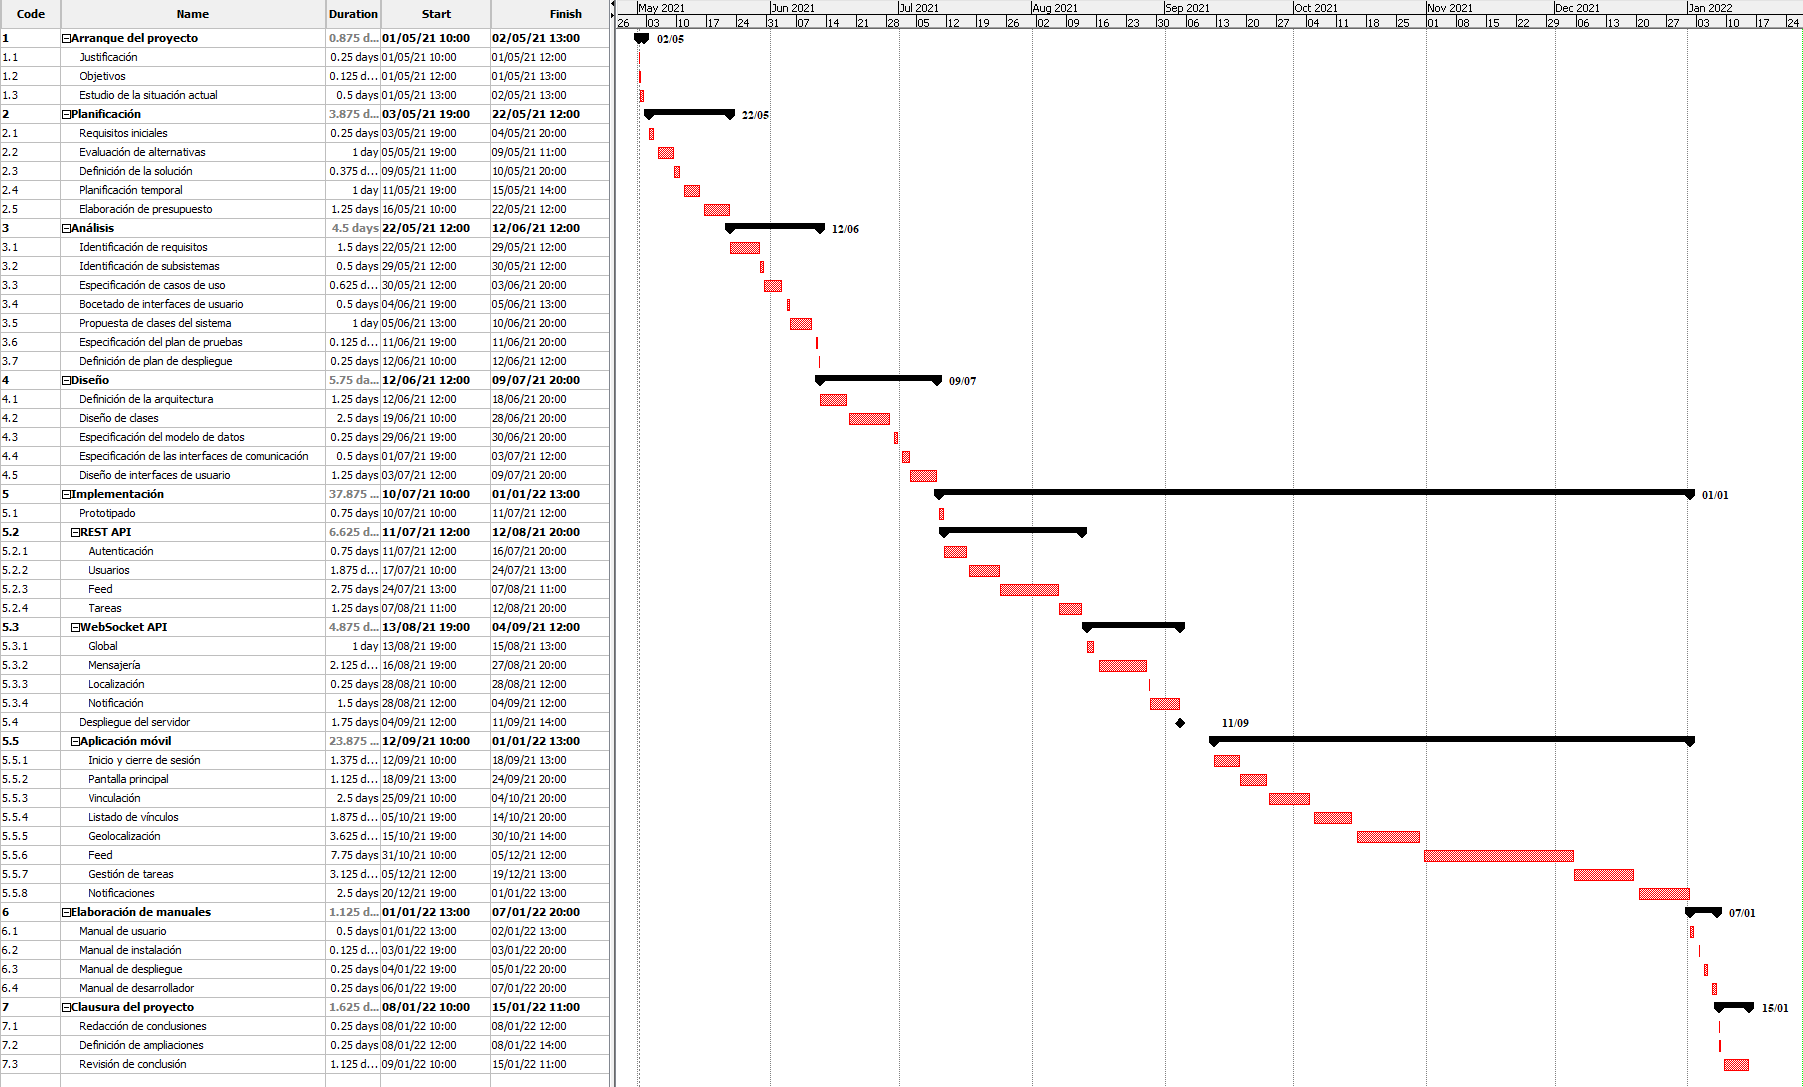
\includegraphics[width=1\textwidth]{images/Anexos/DiagramaGantt.png}
    \caption{Diagrama de Gantt del proyecto}
    \label{dia:gantt}
\end{sidewaysfigure}        
\chapter{Resumen del presupuesto}
\label{ch:resumen_presupuesto}

El desarrollo de este proyecto \textbf{carece de perspectiva comercial o de negocio}. No existe ningún porcentaje de beneficio aplicado sobre el coste del proyecto, no se aplica el impuesto de valor añadido y el margen entre el coste total y la facturación se ha reducido a un escueto 1.89\%.

El equipo de desarrollo cuenta con \textbf{un único miembro} y en base a ello se ha considerado el desarrollo como un proyecto \emph{freelance} sin declaración de autónomo. A pesar de existir un único miembro encargado del desarrollo, los costes de las diferentes partidas y tareas se realizaron teniendo en cuenta el cargo que se personará en cada caso concreto en vez de utilizar un único salario y rol general. Los salarios utilizados están basados en las medias encontradas en el portal web Glassdoor\footnote{https://www.glassdoor.es/member/home/index.htm}, con una reducción compensatoria de la inexperiencia del desarrollador.

De cara al cálculo de costes indirectos y de medios de producción del equipo de desarrollo se tomaron en cuenta: el cálculo estimado de consumo eléctrico del portátil usado en el desarrollo, una única licencia de pago\footnote{Licencia de Office 365 para la elaboración del presupuesto con Microsoft Excel} puesto que el resto de softwares utilizados son gratuitos, el coste del despliegue del servidor de prueba durante el desarrollo y el coste por hora en base a la amortización de los teléfonos y ordenador empleados durante el desarrollo y que ya se poseían de antes.

A continuación se ofrece el resumen del presupuesto. El desglose detallado de este y sus partidas se puede encontrar en el \fref{ch:anexo_presupuesto} \nameref{ch:anexo_presupuesto} y en la hoja de cálculo adjunta a este documento y que se indica en el \fref{ch:documentacion_adicional}. Cada partida listada en este resumen contiene también la referencia de su partida detallada en dicho anexo.

\vspace{5pt}
% Presupuesto de costes expandido
\begin{longtable}{ l l l r }
    \hline
    Código & Partida & Desglose & Importe \\
    \hline
    1 & Planificación                                   & \fref{pre:planificacion}  & 1 149.00€ \\
    2 & Análisis                                        & \fref{pre:analisis}       & 1 174.00€ \\
    3 & Diseño                                          & \fref{pre:diseno}         & 1 500.00€ \\
    4 & Construcción                                    & \fref{pre:construccion}   & 6 957.00€ \\
    5 & Formación                                       & \fref{pre:formacion}      & 197.00€ \\ \hline
      & \textbf{TOTAL}                                    &                           & \textbf{10 977.00€} \\
    \hline
    \caption{Resumen de presupuesto}
    \label{pre:cliente}
\end{longtable}

\vspace{-30pt}
El coste total del proyecto es de \textbf{10 977.00€}           

\part{Análisis}                                             
\chapter{Requisitos del sistema}
\label{ch:requisitos}

\section{Identificación de actores del sistema}

\subsection{Paciente}
El \textbf{Paciente} o \textbf{Patient} es la figura base alrededor de la que orbita el sistema. Los Pacientes son los usuarios de la aplicación que serán auxiliados por los Cuidadores. Un paciente podrá tener hasta un máximo de seis Cuidadores.

\subsection{Cuidador}
\label{sec:Cuidador}

Los usuarios de tipo \textbf{Cuidador} o \textbf{Keeper} serán aquellos que usen la aplicación con ánimo de ayudar a un Paciente. Los Cuidadores sólo podrán tener un Paciente vinculado, pero estarán en contacto con los demás Cuidadores de dicho Paciente. 

\subsection{Administración}

Debido a las funciones y carácter cerrado de la aplicación se ha estimado que una figura o rol de administración dentro del sistema sería innecesario. No es necesario ninguna clase de control ni gestión o comprobación a gran escala que exija una moderación interna. Todos los conflictos que puedan surgir por parte de los usuarios podrían ser resueltos por medio de modificaciones directas a la base de datos, que ya cuenta con su propio portal de administración, haciendo innecesario el desarrollo de ningún sistema dedicado para las labores de mantenimiento y administración.

\subsection{Identificación de relación de actores}

Entre los actores relevantes del sistema existen dos tipos de relación que serán nombradas en el documento:

\begin{itemize}
    \item \textbf{Vínculo}. Relación entre un Paciente y un Cuidador que han sido enlazados. Los usuarios vinculados de un Paciente son sus Cuidadores. El único usuario vinculado de un Cuidador es su Paciente.
    \item \textbf{Asociación}. Relación entre Cuidadores del mismo Paciente, súper relación de Vínculo. Los usuarios asociados de un Paciente son sus Cuidadores. Los usuarios asociados de un Cuidador son el resto de Cuidadores del paciente y el propio Paciente.
\end{itemize}

\section{Identificación de requisitos}

\subsection{RSU. Requisitos de sesión de usuario}

\begin{enumerate}[label*=RSU \arabic*.]
    \item Los usuarios podrán iniciar sesión en la aplicación mediante autenticación con su cuenta de Google.
    \item Los inicios de sesión serán validados con una petición a la \acrshort{api} \acrshort{rest} con el \gls{token} obtenido de la validación con Google.
    \begin{enumerate}[label*=\arabic*.]
        \item Si el inicio de sesión es inválido el usuario será notificado del error y se le permitirá reintentarlo.
        \item \label{req:inicio_sesion} Si el inicio de sesión es válido y el usuario ya está registrado, se creará la sesión del usuario.
        \begin{enumerate}[label*=\arabic*.]
            \item \label{req:sesion} La \acrshort{api} \acrshort{rest} creará y almacenará la sesión del usuario. Dicha sesión estará compuesta por:
            \begin{enumerate}[label*=\arabic*.]
                \item \label{req:token_sesion}  \Gls{token} de sesión para realizar las peticiones. Tendrá un tiempo de validez de TIEMPO\textunderscore VALIDEZ\textunderscore TOKEN\textunderscore SESIÓN.
                \item \label{req:token_refresco} \Gls{token} de refresco de sesión para mantener la sesión activa y obtener un nuevo par de \glspl{token}. Tendrá un tiempo de validez de TIEMPO\textunderscore VALIDEZ\textunderscore TOKEN\textunderscore REFRESCO.
            \end{enumerate}
            \item La sesión pasará a ser inválida cuando caduque su \labelcref{req:token_refresco}.
            \item \label{req:info_sesion} La \acrshort{api} \acrshort{rest} enviará a la aplicación la información de sesión del usuario.
            \begin{enumerate}[label*=\arabic*.]
                \item \Gls{token} de sesión (\labelcref{req:token_sesion}).
                \item \Gls{token} de refresco de sesión (\labelcref{req:token_refresco}).
                \item Instante de caducidad de la sesión.
            \end{enumerate}
            \item El usuario será redirigido a la pantalla principal de la aplicación.
        \end{enumerate}
        \item \label{req:registro} Si el inicio de sesión es válido y el usuario es nuevo se le redirigirá a la actividad de creación de usuarios.
        \begin{enumerate}[label*=\arabic*.]
            \item \label{req:nombre_usuario} El usuario deberá indicar un nombre válido.
            \item \label{req:rol_usuario} El usuario deberá seleccionar un rol entre los posibles:
            \begin{enumerate}[label*=\arabic*.]
                \item Paciente
                \item Cuidador
            \end{enumerate}
            \item \label{req:info_adicional} El usuario podrá añadir información adicional a su perfil.
            \begin{itemize}
                \item Teléfono de contacto
                \item Teléfono de contacto alternativo
                \item Dirección de correo electrónico
                \item Dirección física. Conformada por dos campos para componer la dirección postal, un campo para la localidad y un campo para la región.
            \end{itemize}
            \item La aplicación pedirá confirmación al usuario de los datos insertados.
            \begin{enumerate}[label*=\arabic*.]
                \item Si el usuario confirma los datos insertados, los datos serán enviados a la \acrshort{api} \acrshort{rest} para su almacenamiento y validación.
                \item Si el usuario no es válido, la \acrshort{api} \acrshort{rest} responderá con un mensaje de error.
                \item Si el usuario es válido, la \acrshort{api} \acrshort{rest} responderá a la petición con un mensaje de éxito y el perfil completo del usuario.
                \item Tras la creación exitosa del perfil, el usuario será dado de alta siguiendo \labelcref{req:inicio_sesion}.
            \end{enumerate}
        \end{enumerate}
        \item La sesión podrá ser renovada con una solicitud a la \acrshort{api} \acrshort{rest} con el \gls{token} de refresco de sesión mientras este siga siendo válido.
            \begin{enumerate}[label*=\arabic*.]
                \item Refrescar una sesión generará una tupla como la de \labelcref{req:sesion} y sustituirá la almacenada anteriormente.
                \item La \acrshort{api} \acrshort{rest} responderá con la información de la sesión de usuario como en \labelcref{req:info_sesion}.
                \item Al refrescar una sesión los \glspl{token} anteriores quedarán invalidados.
            \end{enumerate}
    \end{enumerate}
    \item \label{req:cierre_sesion} Los usuarios con la sesión iniciada podrán cerrar sesión en la aplicación.
    \begin{enumerate}[label*=\arabic*.]
        \item La aplicación enviará la petición de cierre de sesión a la \acrshort{api} \acrshort{rest} con el \gls{token} de autenticación.
        \item La \acrshort{api} \acrshort{rest} eliminará la sesión almacenada y confirmará la acción a la aplicación.
        \item Si el cierre de sesión es exitoso el usuario será redirigido a la pantalla de inicio de sesión.
    \end{enumerate}
\end{enumerate}

\subsection{RGU. Requisitos de gestión de usuarios}

\begin{enumerate}[label*=RGU \arabic*.]
    \item \label{req:consultar_info_paciente} Los usuarios podrán ver la información del Paciente vinculado en la pantalla principal.
    \begin{enumerate}[label*=\arabic*.]
        \item La información a mostrar será suministrada por la \acrshort{api} \acrshort{rest}.
        \item En el caso de Pacientes se les mostrará su propia información.
        \item La información mostrada será:
        \begin{itemize}
            \item Nombre.
            \item Teléfono de contacto.
            \item Teléfono de contacto alternativo.
            \item Dirección de correo electrónico.
            \item Dirección postal.
        \end{itemize}
        \item \label{req:accion_contactos} Los datos de contacto de la tarjeta proporcionarán atajos para usarlos:
        \begin{enumerate}[label*=\arabic*.]
            \item Los números de teléfono desplegarán el dial del teléfono con el número marcado.
            \item El correo electrónico abrirá una aplicación de correo electrónico con un nuevo correo preparado para ser enviado a la dirección.
            \item La dirección postal desplegará Google Maps con la dirección ya buscada.
        \end{enumerate}
    \end{enumerate}
    \item Los usuarios podrán actualizar su información.
    \begin{enumerate}[label*=\arabic*.]
        \item El usuario actualizará los campos que prefiera de:
        \begin{itemize}
            \item Nombre.
            \item Teléfono de contacto.
            \item Teléfono de contacto alternativo.
            \item Dirección de correo electrónico.
            \item Dirección postal.
        \end{itemize}
        \item Cuando el usuario confirme la actualización, los datos serán enviados a la \acrshort{api} \acrshort{rest} para validación.
        \item La \acrshort{api} \acrshort{rest} confirmará los cambios efectuados y responderá con la información completa del usuario.
        \item La aplicación se actualizará con los nuevos datos del usuario.
        \item \label{req:noti_actualizar} Una notificación será enviada a los usuarios vinculados acerca de la actualización de los datos del usuario.
    \end{enumerate}
    \item La aplicación permitirá a los usuarios establecer vínculos con otros usuarios.
    \begin{enumerate}[label*=\arabic*.]
        \item Los Pacientes podrán vincular MAX\textunderscore VINCULOS\textunderscore PACIENTE usuarios de tipo Cuidador.
        \item Los Cuidadores podrán vincular MAX\textunderscore VINCULOS\textunderscore CUIDADOR Pacientes.
        \item \label{req:vinculo_paciente} Los Pacientes podrán generar un código QR para vincularse.
        \begin{enumerate}[label*=\arabic*.]
            \item El código QR representará un token provisto por la \acrshort{api} \acrshort{rest}.
            \item El token caducará en TIEMPO\textunderscore CADUCIDAD\textunderscore TOKEN\textunderscore VINCULACIÓN.
        \end{enumerate}
        \item \label{req:vinculo_cuidador} Los Cuidadores podrán escanear el código QR de un Paciente para completar el vínculo.
        \begin{enumerate}[label*=\arabic*.]
            \item El código leído será enviado a la \acrshort{api} \acrshort{rest}.
            \item La \acrshort{api} \acrshort{rest} validará el token y que el vínculo sea válido.
            \begin{enumerate}[label*=\arabic*.]
                \item Si el vínculo no es válido, una respuesta de error será emitida
                \item Si el vínculo es válido, se creará el vínculo entre ambos usuarios.
            \end{enumerate}
        \end{enumerate}
        \item \label{req:noti_nuevo_vinculo} La \acrshort{api} \acrshort{rest} emitirá una notificación de la creación del vínculo al resto de usuarios asociados.
    \end{enumerate}
    \item \label{req:borrar_vinculo} Los usuarios con vínculos activos podrán eliminar sus vínculos actuales a través de la aplicación.
    \begin{enumerate}[label*=\arabic*.]
        \item La petición se realizará con una llamada a la \acrshort{api} \acrshort{rest}.
        \item La \acrshort{api} \acrshort{rest} validará la petición y enviará una respuesta de confirmación.
        \item La \acrshort{api} \acrshort{rest} emitirá una notificación de la eliminación del vínculo al resto de usuarios asociados antes de la eliminación del vínculo.
    \end{enumerate}
    \item \label{req:consultar_info_cuidador} La aplicación permitirá listar en la aplicación los Cuidadores relacionados de los usuarios.
    \begin{enumerate}[label*=\arabic*.]
        \item La aplicación listará a los Pacientes sus Cuidadores vinculados.
        \item La aplicación listará a los Cuidadores el resto de Cuidadores vinculados por su Paciente.
        \item El listado de Cuidadores será proporcionado por una petición a la \acrshort{api} \acrshort{rest}.
        \item Con cada Cuidador listado se mostrará su información de contacto:
        \begin{itemize}
            \item Teléfono de contacto.
            \item Teléfono de contacto alternativo.
            \item Dirección de correo electrónico.
            \item Dirección postal.
        \end{itemize}
        \item Desde el listado, la aplicación permitirá a los usuarios los mismos atajos de funcionalidad que \labelcref{req:accion_contactos}.
    \end{enumerate}
\end{enumerate}

\subsection{RGT. Requisitos de gestión de tareas}

\begin{enumerate}[label*=RGT \arabic*.]
    \item \label{req:crear_tarea} Los Pacientes y sus Cuidadores podrán crear una nueva tarea desde la aplicación.
    \begin{enumerate}[label*=\arabic*.]
        \item Las tareas contarán con la siguiente información:
        \begin{enumerate}[label*=\arabic*.]
            \item Un identificador único, obligatorio y generado en el proceso de persistencia de la tarea.
            \item Título, obligatorio.
            \item Creador, obligatorio y rellenado automáticamente por la aplicación.
            \item Descripción, opcional.
            \item Instante de creación, obligatorio y rellenado automáticamente por la aplicación.
            \item Instante de la última actualización, obligatorio y por defecto será creada con el mismo valor que el instante de creación.
            \item Estado de la tarea. Puede ser completa o incompleta. Obligatorio, por defecto será creada como incompleta.
        \end{enumerate}
        \item Las tareas creadas en la aplicación se enviarán a la \acrshort{api} \acrshort{rest} para su validación y persistencia.
        \begin{enumerate}[label*=\arabic*.]
            \item Si la tarea es inválida, la \acrshort{api} \acrshort{rest} emitirá un mensaje de error y no persistirá la tarea.
            \item Si la tarea es válida, la \acrshort{api} \acrshort{rest} responderá con un mensaje de éxito con la información completa de la tarea creada.
        \end{enumerate}
        \item La creación de una tarea la añadirá a la lista de tareas del Paciente involucrado.
        \item \label{req:noti_nueva_tarea} El sistema emitirá una notificación de la tarea creada a los usuarios asociados.
    \end{enumerate}
    \item \label{req:listar_tarea} Los Pacientes y sus Cuidadores podrán consultar las tareas existentes en la aplicación.
    \begin{enumerate}[label*=\arabic*.]
        \item \label{req:tarea_relevancia} La lista de tareas será suministrada por la \acrshort{api} \acrshort{rest}. Se listarán todas las tareas del paciente que se consideren relevantes. Una tarea es relevante si cumple alguna de las siguientes condiciones:
        \begin{enumerate}[label*=\arabic*.]
            \item Si la tarea está incompleta.
            \item Si la última actualización de la tarea entra dentro del margen de días especificado por el usuario.
        \end{enumerate}
        \item \label{req:info_tarea} Las tareas listadas mostrarán el título, el creador, la descripción, el estado y las fechas de creación y actualización.
        \item Las tareas completas e incompletas serán visualmente diferenciables.
        \item Por defecto, las tareas aparecerán listadas de más recientes a más antiguas.
        \item Las tareas se podrán gestionar desde el listado.
    \end{enumerate}
    \item \label{req:marcar_tarea_hecha} Los Pacientes y sus Cuidadores podrán marcar una tarea del Paciente como hecha desde la aplicación.
    \begin{enumerate}[label*=\arabic*.]
        \item El usuario deberá confirmar que quiere marcar la tarea como hecha.
        \item La petición de actualización se hará a la \acrshort{api} \acrshort{rest}, que la validará.
        \begin{enumerate}[label*=\arabic*.]
            \item Si la petición no es válida, la \acrshort{api} \acrshort{rest} emitirá un mensaje de error.
            \item Si la petición es válida, la \acrshort{api} \acrshort{rest} emitirá una respuesta de confirmación.
        \end{enumerate}
        \item La tarea se actualizará visualmente para reflejar su nuevo estado.
        \item La tarea se seguirá mostrando aunque pierda relevancia (véase \labelcref{req:tarea_relevancia}) hasta que la lista sea refrescada. Permitiendo deshacer la acción.
        \item \label{req:noti_tarea_hecha} El sistema notificará el cambio en el estado a los usuarios asociados.
    \end{enumerate}
    \item \label{req:marcar_tarea_no_hecha} Los Pacientes y sus Cuidadores podrán marcar una tarea como no hecha desde la aplicación.
    \begin{enumerate}[label*=\arabic*.]
        \item El usuario deberá confirmar que quiere desmarcar la tarea como hecha.
        \item La petición de actualización se hará a la \acrshort{api} \acrshort{rest}, que la validará.
        \begin{enumerate}[label*=\arabic*.]
            \item Si la petición no es válida, la \acrshort{api} \acrshort{rest} emitirá un mensaje de error.
            \item Si la petición es válida, la \acrshort{api} \acrshort{rest} emitirá una respuesta de confirmación.
        \end{enumerate}
        \item La tarea se actualizará visualmente para reflejar su nuevo estado.
        \item \label{req:noti_tarea_no_hecha} El sistema notificará el cambio en el estado a los usuarios asociados.
    \end{enumerate}
    \item \label{req:eliminar_tarea} Los usuarios podrán eliminar tareas en la aplicación.
    \begin{enumerate}[label*=\arabic*.]
        \item Los Pacientes podrán eliminar cualquiera de sus tareas.
        \item Los Cuidadores sólo podrán eliminar las tareas creadas por ellos.
        \item El usuario deberá confirmar que quiere eliminar la tarea.
        \item La petición de eliminación se hará a la \acrshort{api} \acrshort{rest}, que la validará.
        \begin{enumerate}[label*=\arabic*.]
            \item Si la petición no es válida, la \acrshort{api} \acrshort{rest} emitirá un mensaje de error.
            \item Si la petición es válida, la \acrshort{api} \acrshort{rest} emitirá una respuesta de confirmación.
        \end{enumerate}
        \item \label{req:noti_tarea_eliminada} El sistema notificará a los usuarios vinculados de la eliminación de la tarea.
    \end{enumerate}
\end{enumerate}

\subsection{RSV. Requisitos de servicio de mensajería}

\begin{enumerate}[label*=RSV \arabic*.]
    \item La aplicación ofrecerá una sala de mensajería a los usuarios vinculados.
    \item La aplicación se conectará a un WebSocket de la \acrshort{api} de la sala.
    \item Los participantes de la sala de mensajería serán el Paciente y todos sus Cuidadores vinculados.
    \item Los mensajes de la sala pueden ser de tres tipos:
    \begin{enumerate}[label*=\arabic*.]
        \item Mensajes de texto.
        \item Tareas.
        \item Notificaciones.
    \end{enumerate}
    \item \label{req:listar_mensaje} La sala de mensajería mostrará, a los usuarios que se conecten, los mensajes más recientes.
    \begin{enumerate}[label*=\arabic*.]
        \item Los mensajes al abrir la sala serán servidos por la \acrshort{api} \acrshort{rest}.
        \item La \acrshort{api} \acrshort{rest} servirá los CANTIDAD\textunderscore GRUPO\textunderscore MENSAJES mensajes más recientes.
        \item Los participantes podrán cargar mensajes más antiguos.
        \item Al solicitar mensajes más antiguos la \acrshort{api} \acrshort{rest} servirá los CANTIDAD\textunderscore GRUPO\textunderscore MENSAJES mensajes más recientes siguientes.
        \item La aplicación mostrará los nuevos mensajes entrantes en tiempo real.
        \item Los mensajes entrantes serán servidos a través del WebSocket.
        \item Los mensajes salientes y entrantes serán visualmente diferentes.
        \item Los tipos de mensajes será visualmente diferentes.
        \item Los mensajes serán agrupados por fecha de emisión.
    \end{enumerate}
    \item \label{req:envio_mensaje} Los participantes de una sala de mensajería podrán enviar mensajes de texto al resto de pacientes.
    \begin{enumerate}[label*=\arabic*.]
        \item El mensaje saliente se enviará a través del WebSocket.
        \item La \acrshort{api} persistirá el mensaje y lo reenviará por el WebSocket al resto de participantes.
        \item El mensaje saliente se añadirá a la lista de mensajes mostrados.
    \end{enumerate}
    \item Los participantes de una sala de mensajería podrán gestionar tareas a través de la sala.
    \begin{enumerate}[label*=\arabic*.]
        \item Las tareas serán tratadas como mensajes.
        \item Los participantes podrán crear una tarea que se enviará por la sala de mensajería igual que en \labelcref{req:envio_mensaje}.
        \item Las tareas creadas de esta forma cumplirán las mismas pautas que en \labelcref{req:crear_tarea}
        \item Las tareas mostradas en la sala de mensajería podrán ser marcadas como hechas como en \labelcref{req:marcar_tarea_hecha}
        \item Las tareas mostradas en la sala de mensajería podrán ser desmarcadas como hechas como en \labelcref{req:marcar_tarea_no_hecha}
        \item Las tareas mostradas en la sala de mensajería podrán ser eliminadas como en \labelcref{req:eliminar_tarea}
        \begin{enumerate}[label*=\arabic*.]
            \item Las tareas eliminadas mientras el usuario esté conectado serán eliminadas de la lista.
            \item La eliminación de una tarea por cualquier medio será comunicada a los usuarios conectados a la sala con una notificación.
        \end{enumerate}
        \item Las acciones sobre las tareas de la sala serán enviadas a la API a través del WebSocket.
        \item La \acrshort{api} ejecutará la petición y enviará un mensaje al resto de participantes de la sala que actualice la tarea.
    \end{enumerate}
    \item Los participantes serán desconectados del WebSocket de la sala al abandonarla.
    \item La sala de mensajería mostrará notificaciones de la conexión y desconexión de usuarios de la sala al resto de usuarios conectados.
\end{enumerate}

\subsection{RSG. Requisitos del sistema de geolocalización}

\begin{enumerate}[label*=RSG \arabic*.]
    \item La aplicación servirá un mapa con un servicio de geolocalización mutua entre usuarios conectados.
    \item La aplicación utilizará la \acrshort{api} de Google Maps.
    \item \label{req:compartir_ubicacion} A través de la aplicación los usuarios podrán compartir su ubicación.
    \begin{enumerate}[label*=\arabic*.]
        \item La aplicación solicitará permiso al usuario para utilizar el \acrshort{gps} integrado en el teléfono móvil.
        \begin{enumerate}[label*=\arabic*.]
            \item Si el usuario deniega acceso al \acrshort{gps}, un mensaje de error será mostrado y la función no se llevará a cabo.
            \item Si el usuario permite el acceso, se empezará a compartir la ubicación y se mostrará el mapa.
        \end{enumerate}
        \item La aplicación se conectará a un WebSocket compartido con el resto de usuarios relacionados.
        \item La ubicación comenzará a compartirse automáticamente al iniciar el servicio de geolocalización.
        \item La ubicación del usuario será enviada a la \acrshort{api} través del WebSocket en intervalos regulares de INTERVALO\textunderscore COMPARTIR\textunderscore UBICACIÓN.
        \item La posición actual del usuario se mostrará en un mapa.
        \item Cada actualización de la ubicación del usuario modificará su posición visual en el mapa.
        \item \label{req:noti_ubicacion_empezar} Cuando un usuario empiece a compartir su ubicación, una notificación será enviada al resto de usuarios conectados.
    \end{enumerate}
    \item Los usuarios compartiendo ubicación podrán dejar de hacerlo abandonando el mapa del servicio.
    \begin{enumerate}[label*=\arabic*.]
        \item Si un usuario abandona el servicio, la aplicación se desconectará del WebSocket.
        \item\label{req:noti_ubicacion_parar}  Cuando un usuario se desconecta del servicio, una notificación será enviada al resto de usuarios conectados.
        \item La notificación de un usuario dejando de compartir su ubicación eliminará la notificación previa del comienzo de la función.
    \end{enumerate}
    \item \label{req:ver_ubicaciones} Los usuarios conectados al servicio podrán ver la ubicación de otros usuarios conectados.
    \begin{enumerate}[label*=\arabic*.]
        \item Las ubicaciones ajenas se recibirán en tiempo real.
        \item Las ubicaciones del resto de usuarios se recibirán a través del WebSocket.
        \item La aplicación mostrará un aviso en pantalla cuando la lista de usuarios conectados al servicio cambie. 
        \begin{enumerate}[label*=\arabic*.]
            \item Cuando un usuario entre al servicio.
            \item Cuando un usuario abandone el servicio.
        \end{enumerate}
        \item Las ubicaciones del resto de usuarios se mostrará con un marcador diferenciado.
        \begin{enumerate}[label*=\arabic*.]
            \item El marcador contendrá la información del usuario respectivo.
            \item La actualización de las ubicaciones desplazará el marcador asociado al usuario a la nueva ubicación.
            \item Cuando un usuario se desconecte, su marcador será retirado del mapa.
        \end{enumerate}
    \end{enumerate}
    \item Los usuarios podrán desplazarse por el mapa.
    \item Los usuarios podrán hacer acercar o alejar la vista en el mapa.
    \item Los usuarios podrán centrar el mapa sobre su ubicación.
\end{enumerate}

\subsection{RSN: Requisitos del sistema de notificaciones}

\begin{enumerate}[label*=RSN \arabic*.]
    \item \label{req:notificaciones} La aplicación notificará a los usuarios acerca de diversos sucesos de interés.
    \begin{enumerate}[label*=\arabic*.]
        \item Un nuevo vínculo genera un nuevo usuario asociado (véase \labelcref{req:noti_nuevo_vinculo})
        \item Un usuario asociado ha actualizado sus datos personales (véase \labelcref{req:noti_actualizar})
        \item Un usuario asociado ha creado una nueva tarea (véase \labelcref{req:noti_nueva_tarea}).
        \item Un usuario asociado ha eliminado una tarea (véase \labelcref{req:noti_tarea_eliminada}).
        \item Un usuario asociado ha marcado una tarea como hecha (véase \labelcref{req:noti_tarea_hecha}).
        \item Un usuario asociado ha desmarcado una tarea como hecha (véase \labelcref{req:noti_tarea_no_hecha}).
        \item Un usuario asociado ha comenzado a compartir su ubicación (véase \labelcref{req:noti_ubicacion_empezar}).
        \item Un usuario asociado ha dejado de compartir su ubicación (véase \labelcref{req:noti_ubicacion_parar}).
    \end{enumerate}
    \item La aplicación se unirá a un WebSocket para recibir las notificaciones.
    \item Las notificaciones pueden ser pendientes o no, dependiendo de si el usuario las ha leído.
    \item La aplicación mostrará la cantidad de notificaciones pendientes del usuario.
    \item \label{req:consultar_notificaciones} El usuario podrá ver en la aplicación sus notificaciones pendientes:
    \begin{enumerate}[label*=\arabic*.]
        \item La lista de notificaciones será servida por la \acrshort{api} \acrshort{rest}.
        \item Las notificaciones aparecerán agrupadas por fecha de emisión.
        \item \label{req:leer_notificaciones} Las notificaciones podrán ser marcadas como leídas individualmente o todas a la vez.
        \item Las notificaciones referentes a funciones de la aplicación podrán ser usadas para navegar a dicha función.
    \end{enumerate}
\end{enumerate}

\subsection{RNF: Requisitos no funcionales}

\begin{enumerate}[label*=RNF \arabic*.]
    \item La aplicación estará disponible en Android 8.1 y versiones posteriores del sistema operativo.
    \item La aplicación estará disponible en los siguientes idiomas:
    \begin{itemize}
        \item Inglés
        \item Español
        \item Gallego
    \end{itemize}
    \item La \acrshort{api} debe estar alojada en la nube.
    \begin{enumerate}[label*=\arabic*.]
        \item El sistema de la nube de alojamiento debe ser Microsoft Azure.
        \item La disponibilidad de la API debe ser superior al 99\%. Esto corresponde a una disponibilidad de 8672 horas y 24 minutos por año.
        \item La velocidad de respuesta a peticiones de la \acrshort{api} no debe exceder los TIEMPO\textunderscore MAXIMO\textunderscore RESPUESTA\textunderscore API.
    \end{enumerate}
    \item La base de datos debe estar alojada en la nube.
    \begin{enumerate}[label*=\arabic*.]
        \item El sistema de base de datos en la nube debe ser MongoDB Atlas.
        \item La disponibilidad de la base de datos debe ser superior al 99\%. Esto corresponde a una disponibilidad de 8672 horas y 24 minutos por año.
    \end{enumerate}
    \item El sistema conectará con las siguientes \acrshort{api}s de terceros:
    \begin{enumerate}[label*=\arabic*.]
        \item Google OAuth 2.0.
        \item Google Maps for Android.
    \end{enumerate}
    \item Los usuarios únicamente necesitarán un conocimiento mínimo en el manejo de móviles inteligentes.
\end{enumerate}

\subsection{Valores de requisitos}

\begin{table}[H]
    \centering
    \begin{tabular}{l|l}
    ID & Valor \\ \hline 
    CANTIDAD\textunderscore GRUPO\textunderscore MENSAJES & 30 \\ 
    INTERVALO\textunderscore COMPARTIR\textunderscore UBICACIÓN & 5 segundos \\  
    MAX\textunderscore VINCULOS\textunderscore CUIDADOR & 1 \\
    MAX\textunderscore VINCULOS\textunderscore PACIENTE & 6 \\     
    TIEMPO\textunderscore MAXIMO\textunderscore RESPUESTA\textunderscore API & 10 segundos \\ 
    TIEMPO\textunderscore VALIDEZ\textunderscore TOKEN\textunderscore SESIÓN & 1 hora \\ 
    TIEMPO\textunderscore VALIDEZ\textunderscore TOKEN\textunderscore REFRESCO & 24 horas \\
    TIEMPO\textunderscore VALIDEZ\textunderscore TOKEN\textunderscore VINCULACION & 1 minuto
    \end{tabular}
    \caption{Valores especificados en requisitos}
\end{table}


\chapter{Identificación de subsistemas}
\label{ch:subsistemas}

En base a los requisitos elaborados y al plan de diseño y arquitectura sopesados para el sistema se han identificado los siguientes subsistemas internos a los dos subsistemas mayores del sistema: la aplicación móvil y la \acrshort{api}. Así como la comunicación entre dichos subsistemas y sus subsistemas internos.

\section{Aplicación móvil}
\label{sec:subsistema_app}

De cara a seguir las principales indicaciones en el desarrollo de sistemas Android, se ha decidido utilizar la arquitectura \acrshort{mvvm}\cite{mvvm2021} y, por consiguiente, su misma especificación de subsistemas.

\subsection{Actividades}

Las actividades conforman los mayores componentes de una aplicación Android pues gestionan las pantallas mostradas al usuario y toda lógica de estados y funcionalidad ofrecida por dicha pantalla. Con la aplicación de la arquitectura \acrshort{mvvm} estos componentes se componen a su vez de dos subsistemas interrelacionados.

\subsubsection{Modelos de vista}

Los modelos de vista suponen la novedad introducida por la arquitectura a utilizar y son módulos encargados de extraer la lógica de datos de las actividades para separarlos de la vista. El modelo de vista contiene la información que se mostrará en pantalla o que sea necesaria para la ejecución de la aplicación, y de la misma forma está a cargo de la obtención de esta, gestionando la comunicación con subsistemas inferiores.

\subsubsection{Vistas}

Las vistas son el sistema en control de la lógica de dibujado, animación y manejo de los elementos de la interfaz de usuario. Recuperan la información contenida en sus modelos de vista y la muestran por pantalla. Están compuestas por archivos de diseño de la interfaz y por archivos de código para las gestiones más complejas de la misma.

\subsection{Modelo}

La representación de las entidades de datos a manejar en la aplicación. Son las entidades que se usarán en la comunicación entre subsistemas y carecerán de más responsabilidades que la de manejarse a sí mismas.

\subsection{Repositorios}

Capa de comunicación entre las actividades y los servicios o bases de datos. Tendrán la responsabilidad de comunicarse con los módulos necesarios para obtener los datos solicitados por las actividades y de la transformación de los mismos en los modelos que serán usados en la aplicación. También gestionarán las peticiones en la dirección contraria, solicitando a los servicios acciones sobre entidades proporcionadas por las actividades.

\subsection{Servicios}

Los servicios son la capa más profunda de la aplicación y son los encargados de la comunicación directa con las bases de datos o interfaces web. En el primer planteamiento de la aplicación no se ha estimado la presencia de una base de datos local por lo que los únicos servicios serán todos web. Sin embargo, dentro de los servicios web podremos distinguir dos tipos: unos enfocados en la comunicación \acrshort{http} y otros en la comunicación por medio del protocolo WebSocket.

\section{API}

Para la \acrshort{api} se ha distinguido un total de tres subsistemas mayores relacionados mutuamente en un esquema triangular que invalida el planteamiento de arquitecturas por capas.

\subsection{Bases de datos}

El subsistema a cargo de gestionar la persistencia y recuperación de datos estará compuesto por dos partes interrelacionadas:

\subsubsection{Modelo}

Los modelos serán la representación de las entidades almacenadas en la base de datos y que serán recuperadas por los dos subsistemas superiores. Carecen de toda lógica que no implique su autogestión y serán siempre modificados, creados, leídos o eliminados por los servicios.

\subsubsection{Servicios}

Sistema de gestión del Modelo de la base de datos. Módulos encargados de manejar las consultas y operaciones de la base de datos con toda la lógica necesaria para aseverar la consistencia y restricciones necesarias en los datos. Son el único sistema con capacidad de manejo sobre el Modelo.

\subsection{Manejador HTTP REST}

Módulo a cargo de recibir y gestionar las peticiones \acrshort{http} para la \acrshort{api} \acrshort{rest}. Contiene la lógica de las operaciones a realizar para cumplir la petición, de todas las comprobaciones necesarias y del manejo de error de las mismas en caso de que surjan errores o sean incorrectas. Realizan las operaciones concernientes a los datos por medio de los servicios, quedando en la lógica de este manejador únicamente la gestión del flujo de operaciones.

\subsection{Manejador WebSocket}

Similar al manejador \acrshort{http} \acrshort{rest} pero con la diferencia de que este subsistema escucha los mensajes recibidos por medio de la interfaz WebSocket. Contiene la lógica para gestionar los eventos notificados a través del mismo y para responder a estos de vuelta o por retransmisión a través del socket. Como el otro manejador, todas sus operaciones son únicamente llamadas sucesivas a los servicios necesarios.

\section{Comunicación entre subsistemas}

Para satisfacer el funcionamiento total de los subsistemas de la aplicación se ha definido la siguiente comunicación que garantice la integridad de las arquitecturas.

\subsection{Subsistemas internos de la aplicación móvil}

La comunicación de los subsistemas de la aplicación seguirá también la arquitectura \acrshort{mvvm} y como esta define la comunicación entre sus subsistemas. El diagrama \ref{fig:sub-app} que lo representa está basado en el mismo diagrama del artículo de referencia de Google\cite{mvvm2021}.

Dentro de la aplicación la comunicación entre subsistemas será vertical y unidireccional. Las vistas solo serán accedidas por la propia interacción del usuario y a su vez serán las únicas que se comuniquen con sus modelos de vista. Esto se hará por medio de llamadas para la ejecución de operaciones o mediante el patrón observador sobre los datos (usando objetos LiveData\cite{liveData2021} de Android) gestionados y almacenados por el modelo de vista.

El modelo de vista por su parte estará a cargo de proveer cualquier necesidad de la vista y para toda la lógica que implique una comunicación externa o la persistencia o recuperación de datos se servirá de los repositorios. Los repositorios llamarán a los servicios necesarios para que tramiten la petición y recuperar la información necesaria o llevar a cabo la operación encomendada desde el modelo de vista contactando con la API.

\begin{figure}[H]
    \centering
    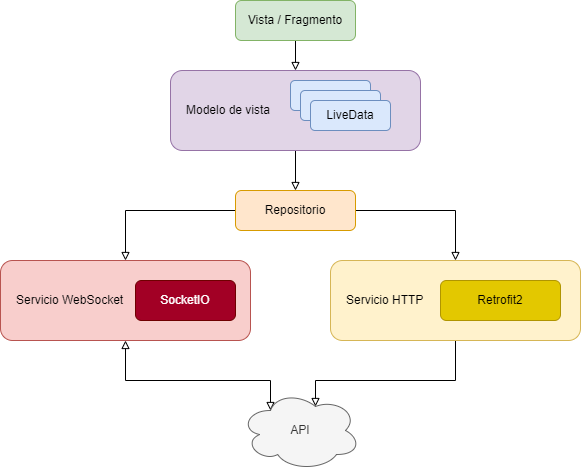
\includegraphics[width=0.6\textwidth]{Analisis/ComunicacionSubsistemasApp.drawio.png}
    \caption{Arquitectura y comunicación de la aplicación móvil}
    \label{fig:sub-app}
\end{figure}

\subsection{Subsistemas internos de la API}

La \acrshort{api} puede recibir comunicaciones por dos vías diferentes. Por peticiones \acrshort{http} a través de su \acrshort{api} \acrshort{rest} y por medio del socket a través de su interfaz WebSocket. A su vez, peticiones \acrshort{http} pueden requerir el envío de eventos a través del socket, por lo que es necesario que exista comunicación entre estos dos subsistemas. Dicha comunicación será llevada a cabo por medio de la referencia recíproca al manejador raíz de ambos subsistemas, de forma que se puedan realizar llamadas mutuas. A su vez, ambos subsistemas requieren la comunicación con la base de datos que realizarán a partir de los servicios.

\begin{figure}[H]
    \centering
    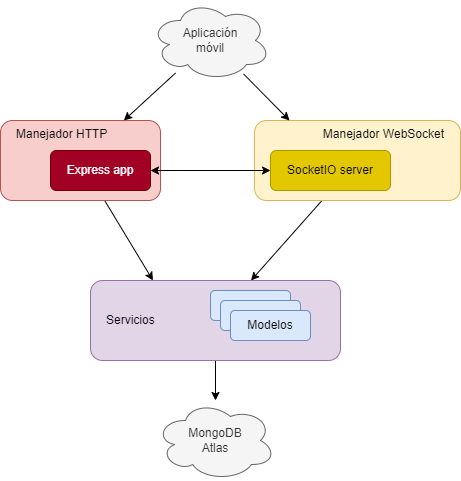
\includegraphics[width=0.4\textwidth]{Analisis/ComunicacionSubsistemasAPI.drawio.png}
    \caption{Arquitectura y comunicación de la API}
    \label{fig:sub-api}
\end{figure}

\subsection{Subsistemas API y aplicación móvil}

Finalmente, de cara a que el sistema funcione se ha definido también la comunicación entre los dos mayores componentes. La comunicación entre la aplicación y la \acrshort{api} tendrá dos vías distintas. Por un lado estarán las peticiones \acrshort{http} realizadas a través de la librería \textbf{Retrofit 2} (\fref{lib:app:retrofit2}) que la \acrshort{api} gestionará y responderá a través de los \gls{endpoint} servidos por medio de su \acrshort{api} \acrshort{rest} construída sobre el framework Express (\fref{lib:api:express}). Y por otro lado, al iniciar la aplicación se establecerá un canal \acrshort{tcp} entre la aplicación y la \acrshort{api} utilizando Socket.IO (\fref{lib:api:socket_io}) en ambos extremos de esta comunicación.

\begin{figure}[H]
    \centering
    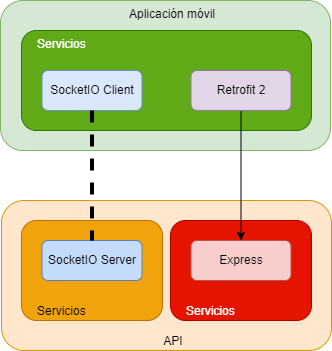
\includegraphics[width=0.3\textwidth]{Analisis/ComunicacionSistemas.drawio.png}
    \caption{Comunicación entre la aplicación y la API}
    \label{fig:sub-comunicacion}
\end{figure}
\chapter{Especificación de casos de uso}
\label{chap:casos_uso}

\section{CU1. Registro}
\label{sec:cu:registro}

\begin{table}[H]
    \centering
    \begin{tabular}{|p{0.25\textwidth} p{0.75\textwidth}|}
    \hline
    \multicolumn{2}{|l|}{\textbf{Caso de Uso 1. Registro}} \\ \hline \hline
    Requisitos          & \labelcref{req:registro} \\ \hline
    Precondiciones      & La cuenta de Google del usuario no debe estar registrada \\ \hline
    Actores             & Usuarios no registrados \\ \hline
    Descripción         & Un usuario nuevo se creará un perfil del sistema e iniciará sesión \\ \hline
    Secuencia normal    & El usuario abrirá la aplicación por primera vez \\
                        & Seleccionará el botón de \emph{Iniciar Sesión} \\
                        & Seleccionará su cuenta de Google \\
                        & Introducirá un nombre para identificarse \\
                        & Elegirá el rol que desee \\
                        & Incluirá su información de contacto adicional \\
                        & Confirmará los datos introducidos \\
                        & El usuario será dirigido a la pantalla principal con un nuevo perfil \\ \hline
    Postcondiciones     & -  \\ \hline
    Excepciones         & Cuenta de Google ya usada: Se iniciará sesión normalmente  \\ \hline
    \end{tabular}
    \caption{Especificación del CU1. Registro}
    \label{cu:registro}
\end{table}

\section{CU2. Iniciar sesión}
\label{sec:cu:iniciar_sesion}

\begin{longtable}{|p{0.25\textwidth} p{0.75\textwidth}|}
    \hline
    \multicolumn{2}{|l|}{\textbf{Caso de Uso 2. Iniciar sesión}} \\ \hline \hline
    Requisitos          & \labelcref{req:inicio_sesion} \\ \hline
    Precondiciones      & El usuario debe disponer de un perfil en el sistema \\ \hline
    Actores             & Pacientes y Cuidadores \\ \hline
    Descripción         & El usuario iniciará sesión con su perfil en el sistema \\ \hline
    Secuencia normal    & El usuario abrirá la aplicación \\
                        & Seleccionará el botón de \emph{Iniciar Sesión} \\
                        & Seleccionará su cuenta de Google \\
                        & El usuario será dirigido a la pantalla principal con su perfil \\ \hline
    Postcondiciones     & - \\ \hline
    Excepciones         & - \\ \hline
    \caption{Especificación del CU2. Iniciar sesión}
    \label{cu:iniciar_sesion}
\end{longtable}

\begin{figure}[H]
    \centering
    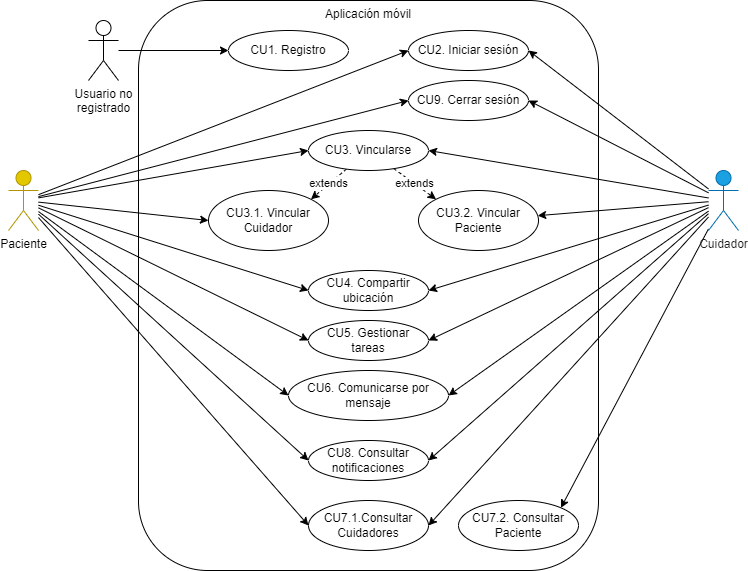
\includegraphics[width=0.85\textwidth]{images/Analisis/CasosUsoGeneral.drawio.png}
    \caption{Diagrama de casos de uso generales}
    \label{fig:casos_uso_general}
\end{figure}

\section{CU3. Vincularse con otro usuario}
\label{sec:cu:vinculacion}

\begin{longtable}{|p{0.25\textwidth} p{0.75\textwidth}|}
    \hline
    \multicolumn{2}{|l|}{\textbf{Caso de Uso 3.1. Vincular un Cuidador}} \\ \hline \hline
    Requisitos          & \labelcref{req:vinculo_paciente} \\ \hline
    Precondiciones      & El usuario debe haber iniciado sesión \\
                        & El Cuidador a vincular debe estar cerca y preparado \\ \hline
    Actores             & Pacientes \\ \hline
    Descripción         & El usuario generará un código para vincularse con un Cuidador \\ \hline
    Secuencia normal    & El usuario seleccionará la función \emph{Forjar vínculo} \\
                        & Un código QR se mostrará en su pantalla \\
                        & El Cuidador lo escaneará \\
                        & Se creará el vínculo entre los usuarios y se notificará a los usuarios asociados \\ \hline
    Postcondiciones     & - \\ \hline
    Excepciones         & El Paciente no puede vincular más Cuidadores: No se forjará el vínculo \\ \hline
    \caption{Especificación del CU3.1. Vincular un Cuidador}
    \label{cu:vincular_cuidador}
\end{longtable}

\begin{longtable}{|p{0.25\textwidth} p{0.75\textwidth}|}
    \hline
    \multicolumn{2}{|l|}{\textbf{Caso de Uso 3.2. Vincular un Paciente}} \\ \hline \hline
    Requisitos          & \labelcref{req:vinculo_cuidador} \\ \hline
    Precondiciones      & El usuario debe haber iniciado sesión \\
                        & El usuario no debe estar ya vinculado \\ 
                        & El Paciente a vincular debe estar cerca y con su código preparado \\ \hline
    Actores             & Cuidadores \\ \hline
    Descripción         & El usuario leerá un código para vincularse con un Paciente \\ \hline
    Secuencia normal    & El usuario seleccionará la función \emph{Forjar vínculo} \\
                        & La aplicación solicitará permisos para utilizar la cámara \\
                        & El usuario aceptará la petición \\
                        & El usuario escaneará el código del Paciente \\
                        & Se creará el vínculo entre los usuarios y se notificará a los asociados \\ \hline
    Postcondiciones     & - \\ \hline
    Excepciones         & No se dan los permisos: La función no se iniciará \\
                        & El Paciente no puede vincular más Cuidadores: No se forjará el vínculo \\ \hline
    \caption{Especificación del CU3.2. Vincular un Paciente}
    \label{cu:vincular_paciente}
\end{longtable}

\begin{longtable}{|p{0.25\textwidth} p{0.75\textwidth}|}
    \hline
    \multicolumn{2}{|l|}{\textbf{Caso de Uso 3.3. Desvincularse}} \\ \hline \hline
    Requisitos          & \labelcref{req:borrar_vinculo} \\ \hline
    Precondiciones      & El usuario debe haber iniciado sesión \\
                        & El usuario debe estar vinculado \\ \hline
    Actores             & Pacientes y Cuidadores \\ \hline
    Descripción         & El usuario eliminará uno de sus vínculos \\ \hline
    Secuencia normal    & El usuario seleccionará la función \emph{Eliminar vínculo} \\
                        & El usuario seleccionará el vínculo a eliminar \\
                        & La aplicación le pedirá confirmación \\
                        & Se eliminará el vínculo entre los usuarios y se notificará a los usuarios asociados \\ \hline
    Postcondiciones     & - \\ \hline
    Excepciones         & - \\ \hline
    \caption{Especificación del CU3.3. Desvincularse}
    \label{cu:desvincular}
\end{longtable}

\section{CU4. Compartir ubicación}
\label{sec:cu:ubicacion}

\begin{longtable}{|p{0.25\textwidth} p{0.75\textwidth}|}
    \hline
    \multicolumn{2}{|l|}{\textbf{Caso de Uso 4.1. Compartir ubicación del usuario}} \\ \hline \hline
    Requisitos          & \labelcref{req:compartir_ubicacion} \\ \hline
    Precondiciones      & El usuario debe haber iniciado sesión \\
                        & El usuario debe estar vinculado \\ \hline
    Actores             & Pacientes y Cuidadores \\ \hline
    Descripción         & El usuario enviará su ubicación actual a los usuarios asociados \\ \hline
    Secuencia normal    & El usuario seleccionará la función \emph{Compartir ubicación} \\
                        & La aplicación solicitará permisos para acceder a la ubicación \\
                        & El usuario aceptará la petición \\
                        & Se desplegará un mapa mostrando la ubicación del usuario \\
                        & Empezará a compartirse la ubicación del usuario y se notificará a los asociados \\ \hline
    Postcondiciones     & - \\ \hline
    Excepciones         & No se dan los permisos: La función no se iniciará \\ \hline
    \caption{Especificación del CU4.1. Compartir ubicación del usuario}
    \label{cu:compartir_ubicacion}
\end{longtable}

\begin{longtable}{|p{0.25\textwidth} p{0.75\textwidth}|}
    \hline
    \multicolumn{2}{|l|}{\textbf{Caso de Uso 4.2. Ver ubicaciones de usuarios asociados}} \\ \hline \hline
    Requisitos          & \labelcref{req:ver_ubicaciones} \\ \hline
    Precondiciones      & El usuario debe haber iniciado sesión \\
                        & El usuario debe estar vinculado \\
                        & Los usuarios asociados deben estar compartiendo su ubicación  \\ \hline
    Actores             & Pacientes y Cuidadores \\ \hline
    Descripción         & La aplicación mostrará al usuario la ubicación de sus usuarios asociados \\ \hline
    Secuencia normal    & El usuario seleccionará la función \emph{Compartir ubicación} \\
                        & El usuario empezará a compartir su ubicación (véase \ref{cu:compartir_ubicacion}) \\
                        & Se desplegará un mapa mostrando la ubicación de los usuarios conectados \\ \hline
    Postcondiciones     & Si el usuario deja de compartir su ubicación no podrá ver las del resto \\ \hline
    Excepciones         & - \\ \hline
    \caption{Especificación del CU4.2. Ver ubicaciones de usuarios asociados}
    \label{cu:ver_ubicaciones}
\end{longtable}

\section{CU5. Gestionar tareas}
\label{sec:cu:tareas}

\begin{longtable}{|p{0.25\textwidth} p{0.75\textwidth}|}
    \hline
    \multicolumn{2}{|l|}{\textbf{Caso de Uso 5.1. Listar tareas}} \\ \hline \hline
    Requisitos          & \labelcref{req:listar_tarea} \\ \hline
    Precondiciones      & El usuario debe haber iniciado sesión \\
                        & Si es Cuidador debe estar vinculado \\ \hline
    Actores             & Pacientes y Cuidadores \\ \hline
    Descripción         & El usuario consultará la lista de tareas relevantes que tiene asociadas \\ \hline
    Secuencia normal    & El usuario seleccionará la pantalla \emph{Tareas} o \emph{Feed} \\
                        & La aplicación recuperarás las tareas relevantes asociadas al usuario \\
                        & Las tareas recuperadas se mostrarán en la pantalla \\ \hline
    Postcondiciones     & - \\ \hline
    Excepciones         & - \\ \hline
    \caption{Especificación del CU5.1. Listar tareas}
    \label{cu:listar_tareas}
\end{longtable}

\begin{longtable}{|p{0.25\textwidth} p{0.75\textwidth}|}
    \hline
    \multicolumn{2}{|l|}{\textbf{Caso de Uso 5.2. Crear tarea}} \\ \hline \hline
    Requisitos          & \labelcref{req:crear_tarea} \\ \hline
    Precondiciones      & El usuario debe haber iniciado sesión \\
                        & Si es Cuidador debe estar vinculado \\ \hline
    Actores             & Pacientes y Cuidadores \\ \hline
    Descripción         & El usuario creará una tarea que se compartirá con los demás usuarios asociados \\ \hline
    Secuencia normal    & El usuario seleccionará la pantalla \emph{Tareas} o \emph{Feed} \\
                        & El usuario seleccionará la función \emph{Crear tarea} \\
                        & El usuario rellenará los campos obligatorios \\
                        & El usuario rellenará los campos opcionales que desee \\
                        & El usuario confirmará la creación de la tarea \\
                        & El sistema creará la tarea y la notificará a los demás usuarios asociados \\ \hline
    Postcondiciones     & - \\ \hline
    Excepciones         & - \\ \hline
    \caption{Especificación del CU5.2. Crear tarea}
    \label{cu:crear_tarea}
\end{longtable}

\begin{longtable}{|p{0.25\textwidth} p{0.75\textwidth}|}
    \hline
    \multicolumn{2}{|l|}{\textbf{Caso de Uso 5.3. Marcar tarea como hecha}} \\ \hline \hline
    Requisitos          & \labelcref{req:marcar_tarea_hecha} \\ \hline
    Precondiciones      & El usuario debe haber iniciado sesión \\
                        & Si es Cuidador debe estar vinculado \\ 
                        & Debe existir alguna tarea no hecha asociada al usuario \\ \hline
    Actores             & Pacientes y Cuidadores \\ \hline
    Descripción         & El usuario marcará una tarea asociada como hecha \\ \hline
    Secuencia normal    & El usuario listará sus tareas, véase CU5.1 (\ref{cu:listar_tareas}) \\
                        & El usuario seleccionará la tarea no hecha que desee \\
                        & El usuario marcará la opción de marcarla hecha \\
                        & La aplicación pedirá confirmación al usuario \\
                        & El usuario confirmará la acción \\
                        & Se modificará la tarea y se notificará a los usuarios asociados \\ \hline
    Postcondiciones     & - \\ \hline
    Excepciones         & - \\ \hline
    \caption{Especificación del CU5.3. Marcar tarea como hecha}
    \label{cu:marcar_tarea}
\end{longtable}

\begin{longtable}{|p{0.25\textwidth} p{0.75\textwidth}|}
    \hline
    \multicolumn{2}{|l|}{\textbf{Caso de Uso 5.4. Desmarcar tarea hecha}} \\ \hline \hline
    Requisitos          & \labelcref{req:marcar_tarea_no_hecha} \\ \hline
    Precondiciones      & El usuario debe haber iniciado sesión \\
                        & Si es Cuidador debe estar vinculado \\ 
                        & Debe existir alguna tarea hecha asociada al usuario \\ \hline
    Actores             & Pacientes y Cuidadores \\ \hline
    Descripción         & El usuario desmarcará una tarea marcada como hecha \\ \hline
    Secuencia normal    & El usuario listará sus tareas, véase CU5.1 (\ref{cu:listar_tareas}) \\
                        & El usuario seleccionará la tarea hecha que desee \\
                        & El usuario marcará la opción de marcarla como no hecha \\
                        & La aplicación pedirá confirmación al usuario \\
                        & El usuario confirmará la acción \\
                        & Se modificará la tarea y se notificará a los usuarios asociados \\ \hline
    Postcondiciones     & - \\ \hline
    Excepciones         & - \\ \hline
    \caption{Especificación del CU5.4. Desmarcar tarea hecha}
    \label{cu:desmarcar_tarea}
\end{longtable}

\begin{longtable}{|p{0.25\textwidth} p{0.75\textwidth}|}
    \hline
    \multicolumn{2}{|l|}{\textbf{Caso de Uso 5.5. Eliminar tarea}} \\ \hline \hline
    Requisitos          & \labelcref{req:eliminar_tarea} \\ \hline
    Precondiciones      & El usuario debe haber iniciado sesión \\
                        & Si es Cuidador debe estar vinculado \\ 
                        & Debe existir alguna tarea asociada al usuario \\ \hline
    Actores             & Pacientes y Cuidadores \\ \hline
    Descripción         & El usuario eliminará una tarea asociada \\ \hline
    Secuencia normal    & El usuario listará sus tareas, véase CU5.1 (\ref{cu:listar_tareas}) \\
                        & El usuario seleccionará la tarea que desee eliminar \\
                        & El usuario elegirá la opción de \emph{Eliminar} la tarea \\
                        & La aplicación pedirá confirmación al usuario \\
                        & El usuario confirmará la acción \\
                        & Se eliminará la tarea y se notificará a los asociados \\ \hline
    Postcondiciones     & - \\ \hline
    Excepciones         & El usuario no es el Paciente o el creador de la tarea: Se le comunicará que es una acción que no puede realizar y no se llevará a cabo \\ \hline
    \caption{Especificación del CU5.5. Eliminar tarea}
    \label{cu:eliminar_tarea}
\end{longtable}

\section{CU6. Comunicarse por mensaje instantáneo}
\label{sec:cu:mensajes}

\begin{longtable}{|p{0.25\textwidth} p{0.75\textwidth}|}
    \hline
    \multicolumn{2}{|l|}{\textbf{Caso de Uso 6.1. Ver mensajes}} \\ \hline \hline
    Requisitos          & \labelcref{req:listar_mensaje} \\ \hline
    Precondiciones      & El usuario debe haber iniciado sesión \\
                        & El usuario debe estar vinculado \\ \hline
    Actores             & Pacientes y Cuidadores \\ \hline
    Descripción         & El usuario verá sus mensajes y tareas asociadas \\ \hline
    Secuencia normal    & El usuario abrirá la pantalla \emph{Feed} \\
                        & La aplicación mostrará los mensajes y tareas asociados al usuario más recientes \\ 
                        & La aplicación mostrará los nuevos mensajes que vayan enviado los usuarios asociados \\ \hline
    Postcondiciones     & - \\ \hline
    Excepciones         & - \\ \hline
    \caption{Especificación del CU6.1. Ver mensajes}
    \label{cu:ver_mensajes}
\end{longtable}

\begin{longtable}{|p{0.25\textwidth} p{0.75\textwidth}|}
    \hline
    \multicolumn{2}{|l|}{\textbf{Caso de Uso 6.2. Enviar mensajes}} \\ \hline \hline
    Requisitos          & \labelcref{req:envio_mensaje} \\ \hline
    Precondiciones      & El usuario debe haber iniciado sesión \\
                        & El usuario debe estar vinculado \\ \hline
    Actores             & Pacientes y Cuidadores \\ \hline
    Descripción         & El usuario verá sus mensajes asociados \\ \hline
    Secuencia normal    & El usuario abrirá la pantalla \emph{Feed} \\
                        & El usuario redactará el mensaje que quiera enviar \\
                        & El usuario pulsará el botón de \emph{Enviar mensaje} \\
                        & El mensaje se listará en la pantalla del usuario \\
                        & El mensaje se enviará al resto de usuarios asociados \\ \hline
    Postcondiciones     & - \\ \hline
    Excepciones         & - \\ \hline
    \caption{Especificación del CU6.2. Enviar mensajes}
    \label{cu:enviar_mensajes}
\end{longtable}

\section{CU7. Consultar información de asociados}

\begin{longtable}{|p{0.25\textwidth} p{0.75\textwidth}|}
    \hline
    \multicolumn{2}{|l|}{\textbf{Caso de Uso 7.1. Consultar Cuidadores asociados}} \\ \hline \hline
    Requisitos          & \labelcref{req:consultar_info_cuidador} \\ \hline
    Precondiciones      & El usuario debe haber iniciado sesión \\
                        & El usuario debe estar vinculado \\ \hline
    Actores             & Pacientes y Cuidadores \\ \hline
    Descripción         & El usuario listará sus Cuidadores asociados y la información de estos \\ \hline
    Secuencia normal    & El usuario abrirá la pantalla \emph{Vínculos} \\
                        & La aplicación obtendrá el listado de los Cuidadores asociados al usuario \\
                        & Los cuidadores asociados se mostrarán en pantalla \\
                        & El usuario desplegará la información del Cuidador que desee para ver su información de contacto completa \\ \hline
    Postcondiciones     & - \\ \hline
    Excepciones         & - \\ \hline
    \caption{Especificación del CU7.1. Consultar Cuidadores asociados}
    \label{cu:consultar_cuidador}
\end{longtable}

\begin{longtable}{|p{0.25\textwidth} p{0.75\textwidth}|}
    \hline
    \multicolumn{2}{|l|}{\textbf{Caso de Uso 7.2. Consultar Paciente asociado}} \\ \hline \hline
    Requisitos          & \labelcref{req:consultar_info_paciente} \\ \hline
    Precondiciones      & El usuario debe haber iniciado sesión \\
                        & El usuario debe estar vinculado \\ \hline
    Actores             & Cuidadores \\ \hline
    Descripción         & El usuario consultará la información de su paciente asociado \\ \hline
    Secuencia normal    & El usuario abrirá la aplicación \\
                        & La aplicación recuperará la información del Paciente \\
                        & Se mostrará en la pantalla principal la información del Paciente \\
                        & El usuario desplegará la información del Paciente para ver su información de contacto completa \\ \hline
    Postcondiciones     & - \\ \hline
    Excepciones         & - \\ \hline
    \caption{Especificación del CU7.2. Consultar Paciente asociado}
    \label{cu:consultar_paciente}
\end{longtable}

\section{CU8. Consultar notificaciones}

\begin{longtable}{|p{0.25\textwidth} p{0.75\textwidth}|}
    \hline
    \multicolumn{2}{|l|}{\textbf{Caso de Uso 8.1 Consultar notificaciones no leídas}} \\ \hline \hline
    Requisitos          & \labelcref{req:consultar_notificaciones} \\ \hline
    Precondiciones      & El usuario debe haber iniciado sesión \\
                        & El usuario debe estar vinculado \\ \hline
    Actores             & Pacientes y Cuidadores \\ \hline
    Descripción         & El usuario consultará las notificaciones no leídas \\ \hline
    Secuencia normal    & El usuario abrirá la pantalla \emph{Notificaciones} \\
                        & La aplicación recuperará las notificaciones no leídas del usuario \\
                        & Las notificaciones recuperadas se mostrarán en la pantalla agrupadas \\ \hline
    Postcondiciones     & - \\ \hline
    Excepciones         & - \\ \hline
    \caption{Especificación del CU8.1 Consultar notificaciones no leídas}
    \label{cu:consultar_notificaciones}
\end{longtable}

\begin{figure}[H]
\begin{longtable}{|p{0.25\textwidth} p{0.75\textwidth}|}
    \hline
    \multicolumn{2}{|l|}{\textbf{Caso de Uso 8.2 Marcar notificaciones como leídas}} \\ \hline \hline
    Requisitos          & \labelcref{req:leer_notificaciones} \\ \hline
    Precondiciones      & El usuario debe haber iniciado sesión \\
                        & El usuario debe estar vinculado \\
                        & El usuario debe tener notificaciones pendientes no leídas \\ \hline
    Actores             & Pacientes y Cuidadores \\ \hline
    Descripción         & El usuario marcará uno o todas sus notificaciones pendientes como leídas \\ \hline
    Secuencia normal    & El usuario listará sus aplicaciones, véase CU8.1 (\ref{cu:consultar_notificaciones}) \\
                        & El usuario usará el botón \emph{Marcar como leída} de una notificación o \emph{Marcar todas como leídas} \\
                        & La notificación se marcará como leídas \\ \hline
    Postcondiciones     & - \\ \hline
    Excepciones         & - \\ \hline
    \caption{Especificación del CU8.2 Marcar notificaciones como leídas}
    \label{cu:marcar_notificaciones}
\end{longtable}
\end{figure}

\section{CU9. Cerrar sesión}

\begin{longtable}{|p{0.25\textwidth} p{0.75\textwidth}|}
    \hline
    \multicolumn{2}{|l|}{\textbf{Caso de Uso 9. Cerrar sesión}} \\ \hline \hline
    Requisitos          & \labelcref{req:cierre_sesion} \\ \hline
    Precondiciones      & El usuario debe haber iniciado sesión \\ \hline
    Actores             & Pacientes y Cuidadores \\ \hline
    Descripción         & El usuario seleccionará la función \emph{Cerrar sesión} \\ \hline
    Secuencia normal    & Se cerrará la sesión y se devolverá al usuario a la pantalla de \emph{Iniciar sesión} \\ \hline
    Postcondiciones     & - \\ \hline
    Excepciones         & - \\ \hline
    \caption{Especificación del CU9. Cerrar sesión}
    \label{cu:cerrar_sesion}
\end{longtable}            
\input{chapters/Analisis/AnálisisInterfazUsuario}              
\chapter{Diagrama de clases}
\label{ch:analisis_diagrama_clases}

En base a los análisis de las secciones anteriores se ha definido una versión preliminar del diseño y arquitectura orientativos del sistema.

\section{Clases de la aplicación}

El conjunto de clases general de la aplicación a desarrollar se encuentra resumido en el diagrama de la \fref{fig:diagrama_clases_app}. Las clases de color rojo representan librerías externas clave de la aplicación.

\begin{figure}[H]
    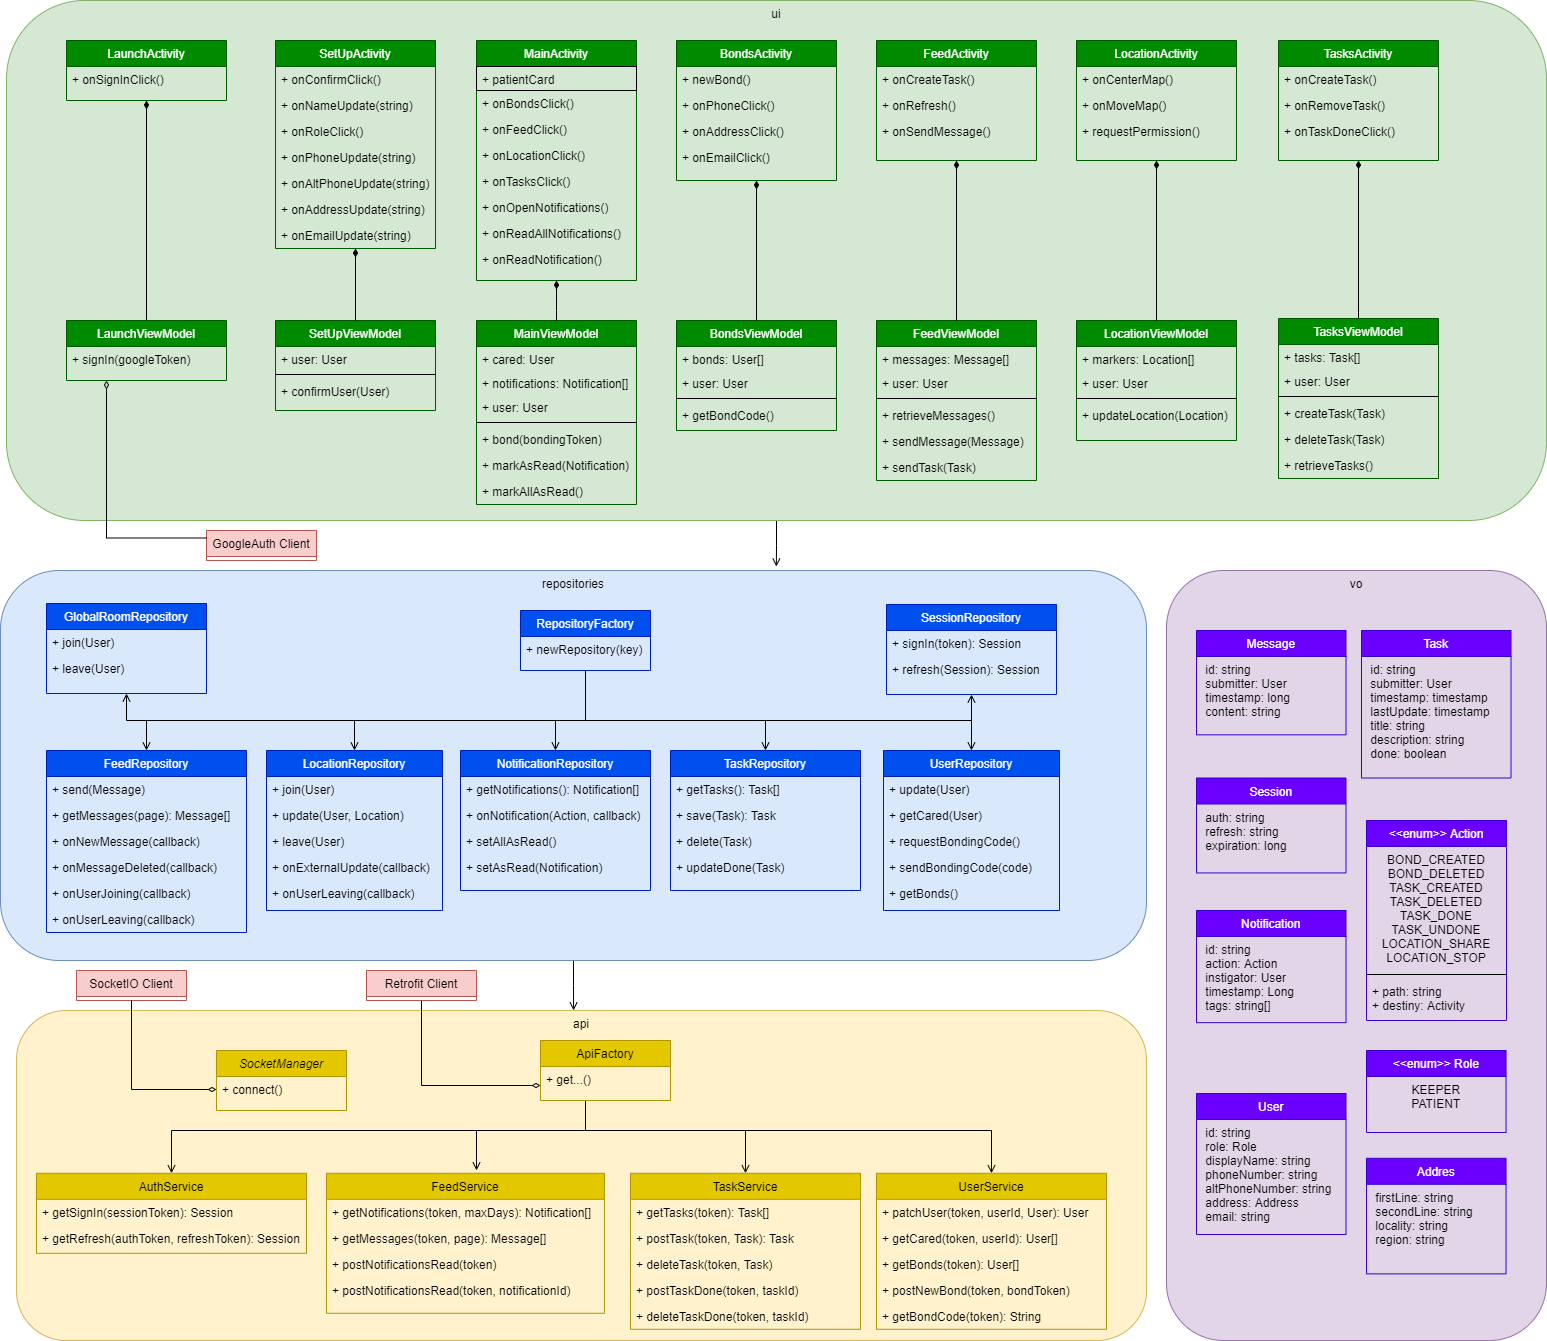
\includegraphics[width=1\textwidth]{images/Analisis/AnalisisDiagramaClasesApp.drawio.png}
    \caption{Diagrama de clases de la Aplicación}
    \label{fig:diagrama_clases_app}
\end{figure}

\subsection{UI}

\vspace{-5pt}
\subsubsection{Launch}

\begin{longtable}{|p{0.25\textwidth} p{0.75\textwidth}|}
    \hline
    \multicolumn{2}{|l|}{LaunchActivity} \\ \hline \hline
    Descripción      & Actividad de inicio de la aplicación con el inicio de sesión \\ \hline
    \multicolumn{2}{|l|}{Funciones} \\
    \emph{onSignClick}  & Arranca el proceso de inicio de sesión  \\ \hline
    \caption{Especificación de la clase LaunchActivity}
    \label{class:app:launch_activity}
\end{longtable}

\vspace{-15pt}
\begin{longtable}{|p{0.25\textwidth} p{0.75\textwidth}|}
    \hline
    \multicolumn{2}{|l|}{LaunchViewModel} \\ \hline \hline
    Descripción      & Modelo de la vista de LaunchActivity \\ \hline
    \multicolumn{2}{|l|}{Funciones} \\
    \emph{signIn}  & Solicita el inicio de sesión a la API  \\ \hline
    \caption{Especificación de la clase LaunchViewModel}
    \label{class:app:launch_view_model}
\end{longtable}

\vspace{-30pt}
\subsubsection{Set up}

\begin{longtable}{|p{0.25\textwidth} p{0.75\textwidth}|}
    \hline
    \multicolumn{2}{|l|}{SetUpActivity} \\ \hline \hline
    Descripción      & Actividad de configuración de la cuenta de usuario en la creación de esta \\ \hline
    \multicolumn{2}{|l|}{Funciones} \\
    \emph{onConfirmClick}  & Confirma la creación del usuario  \\
    \emph{onNameUpdate}  & Actualiza el nombre de usuario  \\ 
    \emph{onRoleClick}  & Selecciona un rol  \\ 
    \emph{onPhoneUpdate}  & Actualiza el número de teléfono principal \\
    \emph{onAltPhoneUpdate}  & Actualiza el número de teléfono alternativo  \\ 
    \emph{onAddressUpdate}  & Actualiza la dirección postal  \\ 
    \emph{onEmailUpdate}  & Actualiza la dirección electrónica  \\  \hline
    \caption{Especificación de la clase SetUpActivity}
    \label{class:app:setup_activity}
\end{longtable}

\vspace{-20pt}
\begin{longtable}{|p{0.25\textwidth} p{0.75\textwidth}|}
    \hline
    \multicolumn{2}{|l|}{SetUpViewModel} \\ \hline \hline
    Descripción      & Modelo de la vista de SetUpActivity \\ \hline
    \multicolumn{2}{|l|}{Propiedades} \\
    \emph{user}  & Información del usuario  \\ \hline
    \multicolumn{2}{|l|}{Funciones} \\
    \emph{confirmUser}  & Envía los datos del usuario para confirmarlo  \\ \hline
    \caption{Especificación de la clase SetUpViewModel}
    \label{class:app:setup_view_model}
\end{longtable}

\subsubsection{Main}

\vspace{-5pt}
\begin{longtable}{|p{0.3\textwidth} p{0.7\textwidth}|}
    \hline
    \multicolumn{2}{|l|}{MainActivity} \\ \hline \hline
    Descripción      & Actividad principal de la aplicación desde la que acceder a todas las funciones con la sesión iniciada \\ \hline
    \multicolumn{2}{|l|}{Propiedades} \\
    \emph{patientCard}  & Tarjeta con la información del Paciente vinculado (\ref{class:app:bonds_activity})  \\ \hline
    \multicolumn{2}{|l|}{Funciones} \\
    \emph{onBondsClick}  & Dirige al usuario a la actividad de vínculos (\ref{class:app:bonds_activity})  \\
    \emph{onFeedClick}  & Dirige al usuario a la actividad del feed (\ref{class:app:feed_activity})  \\ 
    \emph{onLocationClick}  & Dirige al usuario a la actividad de la geolocalización (\ref{class:app:feed_activity})  \\ 
    \emph{onTasksClick}  & Dirige al usuario a la actividad de gestión de tareas (\ref{class:app:tasks_activity})  \\ 
    \emph{onOpenNotifications}  & Despliega las notificaciones de usuario \\ 
    \emph{onReadAllNotifications}  & Marca todas las notificaciones como leídas \\ 
    \emph{onReadNotification}  & Marca una notificación como leída \\ \hline
    \caption{Especificación de la clase MainActivity}
    \label{class:app:main_activity}
\end{longtable}

\vspace{-20pt}
\begin{longtable}{|p{0.25\textwidth} p{0.75\textwidth}|}
    \hline
    \multicolumn{2}{|l|}{MainViewModel} \\ \hline \hline
    Descripción      & Modelo de la vista MainActivity \\ \hline
    \multicolumn{2}{|l|}{Propiedades} \\
    \emph{cared}  & Información del paciente vinculado  \\
    \emph{notifications}  & Lista de notificaciones no leídas del usuario  \\
    \emph{user}  & Información del usuario  \\ \hline
    \multicolumn{2}{|l|}{Funciones} \\
    \emph{bond}  & Envía una petición para crear un vínculo con otro usuario \\
    \emph{markAsRead}  & Envía una petición para marcar una notificación como leída \\ 
    \emph{markAsReadAll}  & Envía una petición para marcar todas las notificación como leída \\ \hline
    \caption{Especificación de la clase MainViewModel}
    \label{class:app:main_view_model}
\end{longtable}

\vspace{-30pt}
\subsubsection{Bonds}

\vspace{-5pt}
\begin{longtable}{|p{0.25\textwidth} p{0.75\textwidth}|}
    \hline
    \multicolumn{2}{|l|}{BondsActivity} \\ \hline \hline
    Descripción      & Actividad para la gestión de los vínculos \\ \hline
    \multicolumn{2}{|l|}{Funciones} \\
    \emph{newBond}  & Dirige al usuario a la actividad de vínculos  \\
    \emph{onPhoneClick}  & Abre la aplicación de teléfono con el número pulsado  \\ 
    \emph{onAddresClick}  & Abre la aplicación de mapas con la dirección pulsada \\ 
    \emph{onEmailClick}  & Abre la aplicación de correo electrónico con el email pulsado \\ \hline
    \caption{Especificación de la clase BondsActivity}
    \label{class:app:bonds_activity}
\end{longtable}

\begin{longtable}{|p{0.25\textwidth} p{0.75\textwidth}|}
    \hline
    \multicolumn{2}{|l|}{BondsViewModel} \\ \hline \hline
    Descripción      & Modelo de la vista BondsActivity \\ \hline
    \multicolumn{2}{|l|}{Propiedades} \\
    \emph{bonds}  & Lista con la información de los usuarios asociados  \\
    \emph{user}  & Información del usuario  \\ \hline
    \multicolumn{2}{|l|}{Funciones} \\
    \emph{getBondCode}  & Envía una petición para obtener un token de vinculación \\ \hline
    \caption{Especificación de la clase BondsViewModel}
    \label{class:app:bonds_view_model}
\end{longtable}

\vspace{-32pt}
\subsubsection{Feed}

\vspace{-7pt}
\begin{longtable}{|p{0.25\textwidth} p{0.75\textwidth}|}
    \hline
    \multicolumn{2}{|l|}{FeedActivity} \\ \hline \hline
    Descripción      & Actividad de la aplicación con el chat entre usuarios asociados \\ \hline
    \multicolumn{2}{|l|}{Funciones} \\
    \emph{onCreateTask}  & Envía el mensaje como tarea \\
    \emph{onRefresh}  & Actualiza la lista de mensajes  \\ 
    \emph{onSendMessage}  & Envía el mensaje  \\ \hline
    \caption{Especificación de la clase FeedActivity}
    \label{class:app:feed_activity}
\end{longtable}

\vspace{-22pt}
\begin{longtable}{|p{0.25\textwidth} p{0.75\textwidth}|}
    \hline
    \multicolumn{2}{|l|}{FeedViewModel} \\ \hline \hline
    Descripción      & Modelo de la vista FeedActivity \\ \hline
    \multicolumn{2}{|l|}{Propiedades} \\
    \emph{messages}  & Lista con los mensajes del Feed  \\
    \emph{user}  & Información del usuario  \\ \hline
    \multicolumn{2}{|l|}{Funciones} \\
    \emph{retrieveMessage}  & Envía una petición para recuperar los mensajes \\
    \emph{sendMessage}  & Envía el mensaje al resto de usuarios \\
    \emph{sendTask}  & Envía la tarea al resto de usuarios \\ \hline
    \caption{Especificación de la clase FeedViewModel}
    \label{class:app:feed_view_model}
\end{longtable}

\vspace{-32pt}
\subsubsection{Location}

\vspace{-7pt}
\begin{longtable}{|p{0.25\textwidth} p{0.75\textwidth}|}
    \hline
    \multicolumn{2}{|l|}{LocationActivity} \\ \hline \hline
    Descripción      & Actividad con el mapa de la geolocalización \\ \hline
    \multicolumn{2}{|l|}{Funciones} \\
    \emph{onCenterMap}  & Centra el mapa en el usuario  \\
    \emph{onMoveMap}  & Mueve el mapa  \\ 
    \emph{requestPermission}  & Solicita el permiso del usuario para usar la geolocalización  \\ \hline
    \caption{Especificación de la clase LocationActivity}
    \label{class:app:location_activity}
\end{longtable}

\begin{longtable}{|p{0.25\textwidth} p{0.75\textwidth}|}
    \hline
    \multicolumn{2}{|l|}{LocationViewModel} \\ \hline \hline
    Descripción      & Modelo de la vista LocationActivity \\ \hline
    \multicolumn{2}{|l|}{Propiedades} \\
    \emph{markers}  & Lista de localizaciones del resto de usuarios  \\
    \emph{user}  & Información del usuario  \\ \hline
    \multicolumn{2}{|l|}{Funciones} \\
    \emph{updateLocation}  & Envía la localización al resto de usuarios \\ \hline
    \caption{Especificación de la clase LocationViewModel}
    \label{class:app:location_view_model}
\end{longtable}

\vspace{-31pt}
\subsubsection{Tasks}

\vspace{-21pt}
\begin{figure}[H]
\begin{longtable}{|p{0.25\textwidth} p{0.75\textwidth}|}
    \hline
    \multicolumn{2}{|l|}{TasksActivity} \\ \hline \hline
    Descripción      & Actividad para la gestión de tareas \\ \hline
    \multicolumn{2}{|l|}{Funciones} \\
    \emph{onCreateTask}  & Confirma la creación de una tarea \\
    \emph{onRemoveTask}  & Elimina una tarea  \\ 
    \emph{onTaskDoneClick}  & Cambia el estado de una tarea  \\ \hline
    \caption{Especificación de la clase TasksActivity}
    \label{class:app:tasks_activity}
\end{longtable}
\end{figure}

\vspace{-21pt}
\begin{longtable}{|p{0.25\textwidth} p{0.75\textwidth}|}
    \hline
    \multicolumn{2}{|l|}{TasksViewModel} \\ \hline \hline
    Descripción      & Modelo de la vista TasksActivity \\ \hline
    \multicolumn{2}{|l|}{Propiedades} \\
    \emph{tasks}  & Lista de tareas relevantes del usuario  \\
    \emph{user}  & Información del usuario  \\ \hline
    \multicolumn{2}{|l|}{Funciones} \\
    \emph{createTask}  & Envía una nueva tarea para crear \\
    \emph{deleteTask}  & Envía una petición para eliminar una tarea \\
    \emph{retrieveTasks}  & Recupera la lista de tareas relevantes del usuario \\ \hline
    \caption{Especificación de la clase TasksViewModel}
    \label{class:app:tasks_view_model}
\end{longtable}

\vspace{-36pt}
\subsection{Repositories}

\vspace{-11pt}
\subsubsection{RepositoryFactory}

\begin{longtable}{|p{0.25\textwidth} p{0.75\textwidth}|}
    \hline
    \multicolumn{2}{|l|}{RepositoryFactory} \\ \hline \hline
    Descripción      & Factoría de repositorios \\ \hline
    \multicolumn{2}{|l|}{Funciones} \\
    \emph{newRepository}  & Genera y devuelve el repositorio solicitado \\ \hline
    \caption{Especificación de la clase RepositoryFactory}
    \label{class:app:repository_factory}
\end{longtable}

\subsubsection{FeedRepository}

\begin{longtable}{|p{0.25\textwidth} p{0.75\textwidth}|}
    \hline
    \multicolumn{2}{|l|}{FeedRepository} \\ \hline \hline
    Descripción      & Repositorio para la gestión de las operaciones relacionadas con el feed \\ \hline
    \multicolumn{2}{|l|}{Funciones} \\
    \emph{send}  & Envía un mensaje \\
    \emph{getMessages}  & Recupera la lista de mensajes \\
    \emph{onNewMessage}  & Suscribe una acción a la entrada de un nuevo mensaje \\
    \emph{onMessageDeleted}  & Suscribe una acción a la eliminación de un mensaje \\
    \emph{onUserJoining}  & Suscribe una acción a la conexión de un usuario a la sala del feed \\
    \emph{onUserLeaving}  & Suscribe una acción a la desconexión de un usuario a la sala del feed \\ \hline
    \caption{Especificación de la clase FeedRepository}
    \label{class:app:feed_repository}
\end{longtable}

\subsubsection{GlobalRoomRepository}

\begin{longtable}{|p{0.25\textwidth} p{0.75\textwidth}|}
    \hline
    \multicolumn{2}{|l|}{GlobalRoomRepository} \\ \hline \hline
    Descripción      & Repositorio para la gestión de la conexión con la sala Global \\ \hline
    \multicolumn{2}{|l|}{Funciones} \\
    \emph{join}  & Conecta al usuario a la sala Global \\
    \emph{leave}  & Desconecta al usuario de la sala Global \\ \hline
    \caption{Especificación de la clase GlobalRoomRepository}
    \label{class:app:global_room_repository}
\end{longtable}

\subsubsection{LocationRepository}

\begin{longtable}{|p{0.25\textwidth} p{0.75\textwidth}|}
    \hline
    \multicolumn{2}{|l|}{LocationRepository} \\ \hline \hline
    Descripción      & Repositorio para operaciones relacionadas con la geolocalización \\ \hline
    \multicolumn{2}{|l|}{Funciones} \\
    \emph{join}  & Suscribe al usuario a la sala de geolocalización \\
    \emph{update}  & Actualiza la localización del usuario \\
    \emph{leave}  & Desconecta al usuario de la sala de geolocalización \\
    \emph{onExternalUpdate}  & Suscribe una acción a la llegada de actualizaciones \\
    \emph{onUserLeaving}  & Suscribe una acción a la desconexión de un usuario \\ \hline
    \caption{Especificación de la clase LocationRepository}
    \label{class:app:location_repository}
\end{longtable}

\subsubsection{NotificationRepository}

\begin{longtable}{|p{0.25\textwidth} p{0.75\textwidth}|}
    \hline
    \multicolumn{2}{|l|}{NotificationRepository} \\ \hline \hline
    Descripción      & Repositorio para operaciones relacionadas con las notificaciones \\ \hline
    \multicolumn{2}{|l|}{Funciones} \\
    \emph{getNotifications}  & Recupera la lista de notificaciones \\
    \emph{onNotification}  & Suscribe una acción a la llegada de una nueva notificación \\
    \emph{setAllAsRead}  & Marca todas las notificaciones como leídas \\
    \emph{setAsRead}  & Marca una notificación como leída \\ \hline
    \caption{Especificación de la clase NotificationRepository}
    \label{class:app:notification_repository}
\end{longtable}

\subsubsection{SessionRepository}

\begin{longtable}{|p{0.25\textwidth} p{0.75\textwidth}|}
    \hline
    \multicolumn{2}{|l|}{SessionRepository} \\ \hline \hline
    Descripción      & Repositorio para operaciones relacionadas con la sesión \\ \hline
    \multicolumn{2}{|l|}{Funciones} \\
    \emph{signIn}  & Inicia la sesión del usuario \\
    \emph{refresh}  & Refresca la sesión del usuario \\ \hline
    \caption{Especificación de la clase SessionRepository}
    \label{class:app:session_repository}
\end{longtable}

\subsubsection{TasksRepository}

\begin{longtable}{|p{0.25\textwidth} p{0.75\textwidth}|}
    \hline
    \multicolumn{2}{|l|}{TasksRepository} \\ \hline \hline
    Descripción      & Repositorio para operaciones relacionadas con las tareas \\ \hline
    \multicolumn{2}{|l|}{Funciones} \\
    \emph{delete}  & Elimina una tarea \\
    \emph{getTasks}  & Recupera las tareas \\
    \emph{save}  & Guarda una tarea \\
    \emph{update}  & Actualiza una tarea \\ \hline
    \caption{Especificación de la clase TasksRepository}
    \label{class:app:tasks_repository}
\end{longtable}

\newpage
\subsubsection{UserRepository}

\begin{longtable}{|p{0.25\textwidth} p{0.75\textwidth}|}
    \hline
    \multicolumn{2}{|l|}{UserRepository} \\ \hline \hline
    Descripción      & Repositorio para operaciones relacionadas con los usuarios \\ \hline
    \multicolumn{2}{|l|}{Funciones} \\
    \emph{update}  & Actualiza los datos del usuario \\
    \emph{getCared}  & Recupera los datos del Paciente vinculado \\
    \emph{requestBondingCode}  & Solicita un token de vinculación \\
    \emph{sendBondingCode}  & Elimina un token de vinculación \\
    \emph{getBonds}  & Recupera los vínculos del usuario \\ \hline
    \caption{Especificación de la clase UserRepository}
    \label{class:app:user_repository}
\end{longtable}

\vspace{-30pt}
\subsection{API}

\vspace{-10pt}
\subsubsection{ApiFactory}

\begin{longtable}{|p{0.25\textwidth} p{0.75\textwidth}|}
    \hline
    \multicolumn{2}{|l|}{ApiFactory} \\ \hline \hline
    Descripción      & Factoría de servicios de la API \\ \hline
    \multicolumn{2}{|l|}{Funciones} \\
    \emph{get}  & Crea y regresa el servicio solicitado \\ \hline
    \caption{Especificación de la clase ApiFactory}
    \label{class:app:api_factory}
\end{longtable}

\vspace{-20pt}
\subsubsection{SocketManager}

\begin{longtable}{|p{0.25\textwidth} p{0.75\textwidth}|}
    \hline
    \multicolumn{2}{|l|}{SocketManager} \\ \hline \hline
    Descripción      & Clase a cargo de la gestión del socket \\ \hline
    \multicolumn{2}{|l|}{Funciones} \\
    \emph{connect}  & Conecta al usuario a la API WebSocket \\ \hline
    \caption{Especificación de la clase SocketManager}
    \label{class:app:socket_manager}
\end{longtable}

\vspace{-20pt}
\subsubsection{AuthService}

\begin{longtable}{|p{0.25\textwidth} p{0.75\textwidth}|}
    \hline
    \multicolumn{2}{|l|}{AuthService} \\ \hline \hline
    Descripción      & Servicio para la realización de peticiones al endpoint /auth \\ \hline
    \multicolumn{2}{|l|}{Funciones} \\
    \emph{getSignIn}  & Realiza una petición a GET /auth/signin \\
    \emph{getRefresh}  & Realiza una petición a GET /auth/refresh \\ \hline
    \caption{Especificación de la clase AuthService}
    \label{class:app:auth_service}
\end{longtable}

\subsubsection{FeedService}

\begin{longtable}{|p{0.25\textwidth} p{0.75\textwidth}|}
    \hline
    \multicolumn{2}{|l|}{FeedService} \\ \hline \hline
    Descripción      & Servicio para la realización de peticiones al endpoint /feed \\ \hline
    \multicolumn{2}{|l|}{Funciones} \\
    \emph{getNotifications}  & Realiza una petición a GET /feed/notification \\
    \emph{getMessages}  & Realiza una petición a GET /feed/message \\
    \emph{postNotificationsRead}  & Realiza una petición a POST /feed/notification/read \\  \hline
    \caption{Especificación de la clase FeedService}
    \label{class:app:feed_service}
\end{longtable}

\subsubsection{TaskService}

\begin{longtable}{|p{0.25\textwidth} p{0.75\textwidth}|}
    \hline
    \multicolumn{2}{|l|}{TaskService} \\ \hline \hline
    Descripción      & Servicio para la realización de peticiones al endpoint /task \\ \hline
    \multicolumn{2}{|l|}{Funciones} \\
    \emph{getTasks}  & Realiza una petición a GET /task \\
    \emph{postTask}  & Realiza una petición a POST /task \\
    \emph{deleteTask}  & Realiza una petición a DELETE /task \\
    \emph{postTaskDone}  & Realiza una petición a POST /task/done \\
    \emph{deleteTaskDone}  & Realiza una petición a DELETE /task/done \\  \hline
    \caption{Especificación de la clase TaskService}
    \label{class:app:task_service}
\end{longtable}

\subsubsection{UserService}

\begin{longtable}{|p{0.25\textwidth} p{0.75\textwidth}|}
    \hline
    \multicolumn{2}{|l|}{UserService} \\ \hline \hline
    Descripción      & Servicio para la realización de peticiones al endpoint /user \\ \hline
    \multicolumn{2}{|l|}{Funciones} \\
    \emph{patchUser}  & Realiza una petición a PATCH /user \\
    \emph{getCared}  & Realiza una petición a GET /user/bond/cared \\
    \emph{getBonds}  & Realiza una petición a GET /user/bond \\
    \emph{postNewBond}  & Realiza una petición a POST /user/bond \\
    \emph{getBondCode}  & Realiza una petición a GET /user/bond \\  \hline
    \caption{Especificación de la clase UserService}
    \label{class:app:user_service}
\end{longtable}

\subsection{VO}

\subsubsection{Message}

\begin{longtable}{|p{0.25\textwidth} p{0.75\textwidth}|}
    \hline
    \multicolumn{2}{|l|}{Message} \\ \hline \hline
    Descripción      & Objeto representante de un mensaje \\ \hline
    \multicolumn{2}{|l|}{Propiedades} \\
    \emph{id}  & Identidad del mensaje \\
    \emph{submitter}  & Usuario que envió el mensaje \\
    \emph{timestamp}  & Instante de creación del mensaje \\
    \emph{content}  & Contenido del mensaje \\  \hline
    \caption{Especificación de la clase Message de la aplicación}
    \label{class:app:message}
\end{longtable}

\subsubsection{Task}

\begin{longtable}{|p{0.25\textwidth} p{0.75\textwidth}|}
    \hline
    \multicolumn{2}{|l|}{Task} \\ \hline \hline
    Descripción      & Objeto representante de una tarea \\ \hline
    \multicolumn{2}{|l|}{Propiedades} \\
    \emph{id}  & ID \\
    \emph{submitter}  & Usuario que envió la tarea \\
    \emph{timestamp}  & Instante de creación del mensaje \\
    \emph{lastUpdate}  & Instante de última actualización del mensaje \\
    \emph{title}  & Título \\
    \emph{description}  & Descripción \\
    \emph{done}  & Estado: hecha o no hecha \\  \hline
    \caption{Especificación de la clase Task de la aplicación}
    \label{class:app:task}
\end{longtable}

\subsubsection{Session}

\begin{longtable}{|p{0.25\textwidth} p{0.75\textwidth}|}
    \hline
    \multicolumn{2}{|l|}{Session} \\ \hline \hline
    Descripción      & Objeto representante de una sesión \\ \hline
    \multicolumn{2}{|l|}{Propiedades} \\
    \emph{auth}  & Token de autenticación \\
    \emph{refresh}  & Token de refresco \\
    \emph{expiration}  & Instante de expiración de la sesión \\  \hline
    \caption{Especificación de la clase Session de la aplicación}
    \label{class:app:session}
\end{longtable}

\subsubsection{Notification}

\begin{longtable}{|p{0.25\textwidth} p{0.75\textwidth}|}
    \hline
    \multicolumn{2}{|l|}{Notification} \\ \hline \hline
    Descripción      & Objeto representante de una notificación \\ \hline
    \multicolumn{2}{|l|}{Propiedades} \\
    \emph{id}  & ID \\
    \emph{action}  & Acción notificada \\
    \emph{instigator} & Usuario que realizó la acción \\
    \emph{timestamp}  & Instante de creación de la notificación \\
    \emph{tags}  & Etiquetas de la notificación \\  \hline
    \caption{Especificación de la clase Notification de la aplicación}
    \label{class:app:notification}
\end{longtable}

\begin{longtable}{|p{0.25\textwidth} p{0.75\textwidth}|}
    \hline
    \multicolumn{2}{|l|}{Action} \\ \hline \hline
    Descripción      & Lista de acciones notificables \\ \hline
    \multicolumn{2}{|l|}{Valores} \\
    \emph{BOND CREATED}  & Creación de un vínculo  \\
    \emph{BOND DELETED}  & Eliminación de un vínculo  \\
    \emph{TASK CREATED}  & Creación de una tarea  \\
    \emph{TASK DELETED}  & Eliminación de una tarea  \\
    \emph{TASK DONE}  & Actualización de una tarea a hecha  \\
    \emph{TASK UNDONE}  & Actualización de una tarea a no hecha  \\
    \emph{LOCATION SHARE}  & Ubicación empezando a ser compartida  \\
    \emph{LOCATION STOP}  & Ubicación dejando de ser compartida  \\ \hline
    \multicolumn{2}{|l|}{Propiedades} \\
    \emph{path}  & Ruta de la notificación \\
    \emph{destiny}  & Actividad destino si la tiene \\  \hline
    \caption{Especificación de la clase Action de la aplicación}
    \label{class:app:action}
\end{longtable}

\newpage
\subsubsection{User}

\begin{longtable}{|p{0.25\textwidth} p{0.75\textwidth}|}
    \hline
    \multicolumn{2}{|l|}{User} \\ \hline \hline
    Descripción      & Objeto representante de un usuario \\ \hline
    \multicolumn{2}{|l|}{Propiedades} \\
    \emph{id}  & ID \\
    \emph{role}  & Rol \\
    \emph{displayName}  & Nombre visible \\
    \emph{phoneNumber}  & Número de teléfono \\
    \emph{altPhoneNumber}  & Número alternativo de teléfono \\
    \emph{address}  & Dirección postal \\
    \emph{email}  & Dirección electrónica \\  \hline
    \caption{Especificación de la clase User de la aplicación}
    \label{class:app:user}
\end{longtable}

\begin{longtable}{|p{0.25\textwidth} p{0.75\textwidth}|}
    \hline
    \multicolumn{2}{|l|}{Role} \\ \hline \hline
    Descripción      & Lista de posibles roles de los usuarios \\ \hline
    \multicolumn{2}{|l|}{Valores} \\
    \emph{PATIENT}  & Pacientes  \\
    \emph{KEEPER}  & Cuidadores  \\ \hline
    \caption{Especificación de la clase Role de la aplicación}
    \label{class:app:role}
\end{longtable}

\begin{longtable}{|p{0.25\textwidth} p{0.75\textwidth}|}
    \hline
    \multicolumn{2}{|l|}{Address} \\ \hline \hline
    Descripción      & Objeto representante de una dirección postal \\ \hline
    \multicolumn{2}{|l|}{Propiedades} \\
    \emph{firstLine}  & Primera línea \\
    \emph{secondLine}  & Segunda línea \\
    \emph{locality}  & Localidad \\
    \emph{region}  & Región \\  \hline
    \caption{Especificación de la clase Address de la aplicación}
    \label{class:app:address}
\end{longtable}

\begin{figure}[H]
    \centering
    \makebox[\textwidth][c]{
        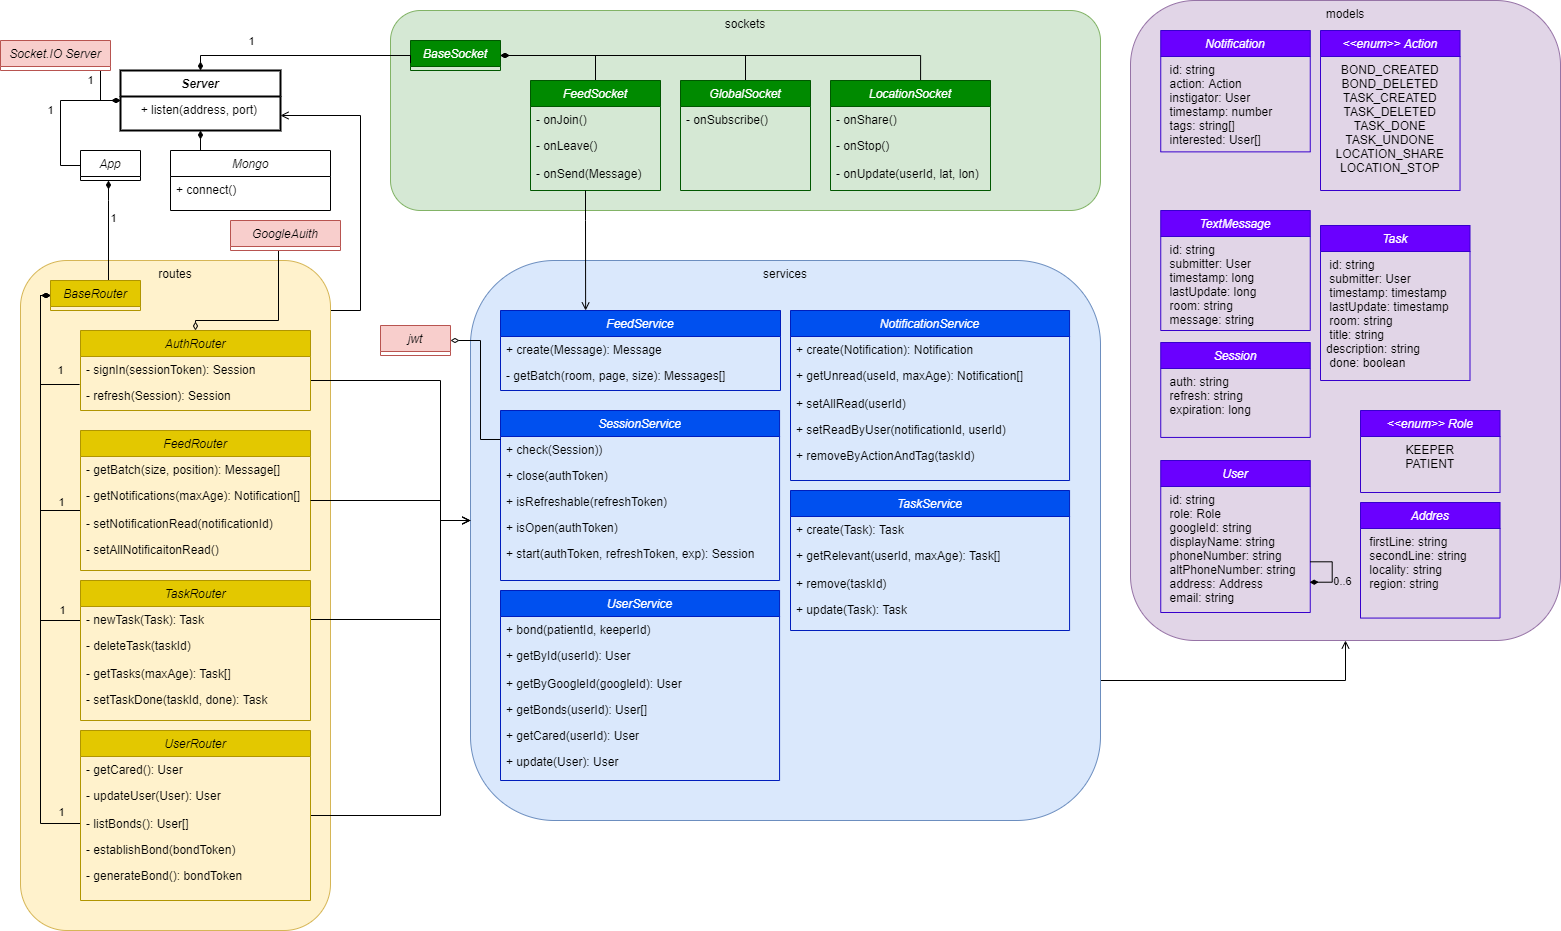
\includegraphics[width=1.2\textwidth]{Analisis/AnalisisDiagramaClasesAPI.drawio.png}
    }
    \caption{Diagrama de clases de la API}
    \label{fig:diagrama_clases_api}
\end{figure}

\section{Clases de la API}

El conjunto de clases general de la API a desarrollar se encuentra resumido en el diagrama de la \ref{fig:diagrama_clases_api}. En el caso de la API los distinto módulos representarán no clases sino paquetes de funciones servidos por sus diferentes índices. Salvo en el caso del paquete de modelos que estará conformado por clases. Los módulos en rojo corresponden a librerías externas ya identificadas.

\subsection{Root}

\begin{longtable}{|p{0.25\textwidth} p{0.75\textwidth}|}
    \hline
    \multicolumn{2}{|l|}{Server} \\ \hline \hline
    Descripción      & Módulo principal y global del sistema. Inicializa todos los sistemas de la API en su lanzamiento desde el punto de entrada de la aplicación \\ \hline
    \multicolumn{2}{|l|}{Funciones} \\
    \emph{listen}  & Despliega el servidor en la direcciones y puerto especificados  \\ \hline
    \caption{Especificación de la clase Server}
    \label{class:api:server}
\end{longtable}

\begin{longtable}{|p{0.25\textwidth} p{0.75\textwidth}|}
    \hline
    \multicolumn{2}{|l|}{App} \\ \hline \hline
    Descripción      & Implementación del servidor Express, punto de entrada de las consultas REST \\ \hline
    \caption{Especificación de la clase App}
    \label{class:api:app}
\end{longtable}

\vspace{-20pt}
\begin{longtable}{|p{0.25\textwidth} p{0.75\textwidth}|}
    \hline
    \multicolumn{2}{|l|}{Mongo} \\ \hline \hline
    Descripción      & Módulo a cargo de la lógica relativa a la conexión de Mongoose con la base de datos \\ \hline
    \multicolumn{2}{|l|}{Funciones} \\
    \emph{connect}  & Crea la conexión con la base de datos remota  \\ \hline
    \caption{Especificación de la clase Mongo}
    \label{class:api:mongo}
\end{longtable}

\vspace{-20pt}
\subsection{Routes}

\begin{longtable}{|p{0.25\textwidth} p{0.75\textwidth}|}
    \hline
    \multicolumn{2}{|l|}{BaseRouter} \\ \hline \hline
    Descripción      & Manejador raíz encargado de redireccionar las peticiones REST al manejador encargado de cada una según la ruta \\ \hline
    \caption{Especificación de la clase BaseRouter}
    \label{class:api:base_router}
\end{longtable}

\vspace{-20pt}
\begin{longtable}{|p{0.25\textwidth} p{0.75\textwidth}|}
    \hline
    \multicolumn{2}{|l|}{AuthRouter} \\ \hline \hline
    Descripción      & Manejador de las peticiones de /auth \\ \hline
    \multicolumn{2}{|l|}{Funciones} \\
    \emph{signIn}  & Crea una sesión para el usuario  \\ 
    \emph{signIn}  & Refresca la sesión del usuario  \\ \hline
    \caption{Especificación de la clase AuthRouter}
    \label{class:api:auth_router}
\end{longtable}

\vspace{-20pt}
\begin{longtable}{|p{0.3\textwidth} p{0.7\textwidth}|}
    \hline
    \multicolumn{2}{|l|}{FeedRouter} \\ \hline \hline
    Descripción      & Manejador de las peticiones de /feed \\ \hline
    \multicolumn{2}{|l|}{Funciones} \\
    \emph{getBatch}  & Devuelve el conjunto de mensajes solicitado por el usuario  \\ 
    \emph{getNotifications}  & Devuelve las notificaciones pendientes del usuario  \\ 
    \emph{setNotificationRead}  & Marcar una notificación como leída  \\ 
    \emph{setAllNotificationsRead}  & Marca todas las notificaciones del usuario como leídas  \\ \hline
    \caption{Especificación de la clase FeedRouter}
    \label{class:api:feed_router}
\end{longtable}

\begin{figure}[H]
\begin{longtable}{|p{0.25\textwidth} p{0.75\textwidth}|}
    \hline
    \multicolumn{2}{|l|}{TaskRouter} \\ \hline \hline
    Descripción      & Manejador de las peticiones de /task \\ \hline
    \multicolumn{2}{|l|}{Funciones} \\
    \emph{newTask}  & Crea una nueva tarea  \\ 
    \emph{deleteTask}  & Elimina la tarea especificada  \\ 
    \emph{getTasks}  & Retorna las tareas relevantes relacionadas con el usuario  \\ 
    \emph{setTaskDone}  & Marca una tarea como hecha/no hecha  \\ \hline
    \caption{Especificación de la clase TaskRouter}
    \label{class:api:task_router}
\end{longtable}
\end{figure}

\vspace{-20pt}
\begin{longtable}{|p{0.25\textwidth} p{0.75\textwidth}|}
    \hline
    \multicolumn{2}{|l|}{UserRouter} \\ \hline \hline
    Descripción      & Manejador de las peticiones de /user \\ \hline
    \multicolumn{2}{|l|}{Funciones} \\
    \emph{getCared}  & Devuelve paciente vinculado con el usuario  \\
    \emph{updateUser}  & Actualiza la información del usuario  \\
    \emph{listBonds}  & Devuelve los vínculos del usuario  \\
    \emph{establishBond}  & Crea un vínculo entre usuarios  \\
    \emph{generateBond}  & Genera un código de vinculación  \\ \hline
    \caption{Especificación de la clase UserRouter}
    \label{class:api:user_router}
\end{longtable}

\vspace{-30pt}
\subsection{Sockets}

\begin{longtable}{|p{0.25\textwidth} p{0.75\textwidth}|}
    \hline
    \multicolumn{2}{|l|}{BaseSocket} \\ \hline \hline
    Descripción      & Manejador raíz encargado de redireccionar los eventos del WebSocket al manejador encargado de cada una según la sala \\ \hline
    \caption{Especificación de la clase BaseSocket}
    \label{class:api:base_socket}
\end{longtable}

\vspace{-20pt}
\begin{longtable}{|p{0.25\textwidth} p{0.75\textwidth}|}
    \hline
    \multicolumn{2}{|l|}{FeedSocket} \\ \hline \hline
    Descripción      & Manejador de la sala del Feed \\ \hline
    \multicolumn{2}{|l|}{Funciones} \\
    \emph{onJoin}  & Gestiona la entrada de un usuario en la sala  \\
    \emph{onLeave}  & Gestione el abandono de la sala de un usuario  \\
    \emph{onSendMessage}  & Maneja el envío de un mensaje  \\ \hline
    \caption{Especificación de la clase FeedSocket}
    \label{class:api:feed_socket}
\end{longtable}

\newpage
\begin{longtable}{|p{0.25\textwidth} p{0.75\textwidth}|}
    \hline
    \multicolumn{2}{|l|}{GlobalSocket} \\ \hline \hline
    Descripción      & Manejador de la sala global \\ \hline
    \multicolumn{2}{|l|}{Funciones} \\
    \emph{onSubscribe}  & Gestiona la suscripción de un usuario a la sala \\ \hline
    \caption{Especificación de la clase GlobalSocket}
    \label{class:api:global_socket}
\end{longtable}

\begin{longtable}{|p{0.25\textwidth} p{0.75\textwidth}|}
    \hline
    \multicolumn{2}{|l|}{LocationSocket} \\ \hline \hline
    Descripción      & Manejador de la sala de la geolocalización \\ \hline
    \multicolumn{2}{|l|}{Funciones} \\
    \emph{onShare}  & Gestiona la entrada de un usuario en la sala  \\
    \emph{onStop}  & Gestione el abandono de la sala de un usuario  \\
    \emph{onUpdate}  & Maneja el envío de una localización  \\ \hline
    \caption{Especificación de la clase LocationSocket}
    \label{class:api:location_socket}
\end{longtable}

\subsection{Services}

\begin{longtable}{|p{0.25\textwidth} p{0.75\textwidth}|}
    \hline
    \multicolumn{2}{|l|}{FeedService} \\ \hline \hline
    Descripción      & Servicio a cargo de los mensajes del feed \\ \hline
    \multicolumn{2}{|l|}{Funciones} \\
    \emph{create}  & Crea y persiste un nuevo mensaje  \\
    \emph{getBatch}  & Devuelve la lista de mensajes especificada  \\ \hline
    \caption{Especificación de la clase FeedService de la API}
    \label{class:api:feed_service}
\end{longtable}

\begin{longtable}{|p{0.3\textwidth} p{0.7\textwidth}|}
    \hline
    \multicolumn{2}{|l|}{NotificationService} \\ \hline \hline
    Descripción      & Servicio a cargo de las notificaciones \\ \hline
    \multicolumn{2}{|l|}{Funciones} \\
    \emph{create}  & Crea y persiste una nueva notificación  \\
    \emph{getUnread}  & Devuelve la lista de notificaciones no leídas de un usuario  \\
    \emph{setAllRead}  & Marca todas las notificaciones de un usuario como leídas  \\
    \emph{setReadByUser}  & Marca una notificación como leída  \\
    \emph{removeByActionAndTag}  & Elimina las notificaciones que tienen la misma acción y etiquetas  \\ \hline
    \caption{Especificación de la clase NotificationService}
    \label{class:api:notification_service}
\end{longtable}

\begin{longtable}{|p{0.25\textwidth} p{0.75\textwidth}|}
    \hline
    \multicolumn{2}{|l|}{SessionService} \\ \hline \hline
    Descripción      & Servicio a cargo de las sesiones de usuario \\ \hline
    \multicolumn{2}{|l|}{Funciones} \\
    \emph{check}  & Comprueba la validez de una sesión  \\
    \emph{close}  & Cierra la sesión especificada  \\
    \emph{isRefreshable}  & Comprueba si una sesión se puede refrescar  \\
    \emph{isOpen}  & Comprueba si una sesión está activa  \\
    \emph{start}  & Crea una nueva sesión de usuario  \\ \hline
    \caption{Especificación de la clase SessionService}
    \label{class:api:session_service}
\end{longtable}

\begin{longtable}{|p{0.25\textwidth} p{0.75\textwidth}|}
    \hline
    \multicolumn{2}{|l|}{TaskService} \\ \hline \hline
    Descripción      & Servicio a cargo de las tareas \\ \hline
    \multicolumn{2}{|l|}{Funciones} \\
    \emph{create}  & Crea y persiste una nueva tarea  \\
    \emph{getRelevant}  & Devuelve la lista de tareas relevantes de un usuario  \\
    \emph{remove}  & Elimina la tarea especificada  \\
    \emph{update}  & Actualiza una tarea  \\ \hline
    \caption{Especificación de la clase TaskService de la API}
    \label{class:api:task_service}
\end{longtable}

\begin{longtable}{|p{0.25\textwidth} p{0.75\textwidth}|}
    \hline
    \multicolumn{2}{|l|}{UserService} \\ \hline \hline
    Descripción      & Servicio a cargo de los datos de usuario \\ \hline
    \multicolumn{2}{|l|}{Funciones} \\
    \emph{bond}  & Crea un vínculo entre usuarios  \\
    \emph{getById}  & Retorna el usuario con la identidad especificada  \\
    \emph{getByGoogleId}  & Retorna el usuario con la identidad de Google especificada  \\
    \emph{getBonds}  & Devuelve los vínculos de un usuario  \\
    \emph{getCared}  & Devuelve el paciente vinculado de un usuario  \\
    \emph{update}  & Actualiza los datos de un usuario  \\ \hline
    \caption{Especificación de la clase UserService de la API}
    \label{class:api:user_service}
\end{longtable}

\newpage
\subsection{Models}

\begin{longtable}{|p{0.25\textwidth} p{0.75\textwidth}|}
    \hline
    \multicolumn{2}{|l|}{Action} \\ \hline \hline
    Descripción      & Lista de posibles acciones notificables \\ \hline
    \multicolumn{2}{|l|}{Valores} \\
    \emph{BOND CREATED}  & Creación de un vínculo  \\
    \emph{BOND DELETED}  & Eliminación de un vínculo  \\
    \emph{TASK CREATED}  & Creación de una tarea  \\
    \emph{TASK DELETED}  & Eliminación de una tarea  \\
    \emph{TASK DONE}  & Actualización de una tarea a hecha  \\
    \emph{TASK UNDONE}  & Actualización de una tarea a no hecha  \\
    \emph{LOCATION SHARE}  & Ubicación empezando a ser compartida  \\
    \emph{LOCATION STOP}  & Ubicación dejando de ser compartida  \\ \hline
    \caption{Especificación de la clase Action de la API}
    \label{class:api:action}
\end{longtable}

\begin{longtable}{|p{0.25\textwidth} p{0.75\textwidth}|}
    \hline
    \multicolumn{2}{|l|}{Address} \\ \hline \hline
    Descripción      & Abstracción de direcciones postales \\ \hline
    \multicolumn{2}{|l|}{Propiedades} \\
    \emph{firstLine}  & Primera línea (por ejemplo, calle y número)  \\
    \emph{secondLine}  & Segunda línea (por ejemplo, piso y puerta)  \\
    \emph{locality}  & Localidad  \\
    \emph{region}  & Región (por ejemplo, provincia o estado)  \\ \hline
    \caption{Especificación de la clase Address de la API}
    \label{class:api:address}
\end{longtable}

\begin{longtable}{|p{0.25\textwidth} p{0.75\textwidth}|}
    \hline
    \multicolumn{2}{|l|}{Notification} \\ \hline \hline
    Descripción      & Entidad representante de las notificaciones de la aplicación \\ \hline
    \multicolumn{2}{|l|}{Propiedades} \\
    \emph{id}  & ID  \\
    \emph{action}  & Acción a notificar  \\
    \emph{instigator}  & Autor de la acción  \\
    \emph{timestamp}  & Instante de realización de la acción  \\
    \emph{tags}  & Etiquetas con información extra de la notificación  \\
    \emph{interested}  & Lista de usuarios receptores de la notificación  \\ \hline
    \caption{Especificación de la clase Notification de la API}
    \label{class:api:notification}
\end{longtable}

\begin{longtable}{|p{0.25\textwidth} p{0.75\textwidth}|}
    \hline
    \multicolumn{2}{|l|}{Role} \\ \hline \hline
    Descripción      & Lista de posibles roles de los usuarios \\ \hline
    \multicolumn{2}{|l|}{Valores} \\
    \emph{PATIENT}  & Pacientes  \\
    \emph{KEEPER}  & Cuidadores  \\ \hline
    \caption{Especificación de la clase Role de la API}
    \label{class:api:role}
\end{longtable}

\begin{longtable}{|p{0.25\textwidth} p{0.75\textwidth}|}
    \hline
    \multicolumn{2}{|l|}{Session} \\ \hline \hline
    Descripción      & Entidad representante de una sesión de usuario \\ \hline
    \multicolumn{2}{|l|}{Propiedades} \\
    \emph{auth}  & Token de autenticación de la sesión  \\
    \emph{refresh}  & Token de refresco de la sesión  \\
    \emph{expiration}  & Instante de expiración de la sesión  \\ \hline
    \caption{Especificación de la clase Session de la API}
    \label{class:api:session}
\end{longtable}

\begin{longtable}{|p{0.25\textwidth} p{0.75\textwidth}|}
    \hline
    \multicolumn{2}{|l|}{Task} \\ \hline \hline
    Descripción      & Entidad representante de las notificaciones de la aplicación \\ \hline
    \multicolumn{2}{|l|}{Propiedades} \\
    \emph{id}  & ID  \\
    \emph{submitter}  & Autor de la tarea  \\
    \emph{timestamp}  & Instante de envío de la tarea \\
    \emph{lastUpdate}  & Última actualización de la tarea  \\
    \emph{room}  & Sala de envío de la tarea  \\
    \emph{title}  & Título  \\
    \emph{description}  & Descripción  \\
    \emph{done}  & Estado: hecha/no hecha  \\ \hline
    \caption{Especificación de la clase Task de la API}
    \label{class:api:task}
\end{longtable}

\newpage
\begin{longtable}{|p{0.25\textwidth} p{0.75\textwidth}|}
    \hline
    \multicolumn{2}{|l|}{TextMessage} \\ \hline \hline
    Descripción      & Entidad representante de los mensajes de texto del Feed \\ \hline
    \multicolumn{2}{|l|}{Propiedades} \\
    \emph{id}  & ID  \\
    \emph{submitter}  & Autor del mensaje  \\
    \emph{timestamp}  & Instante de envío del mensaje \\
    \emph{lastUpdate}  & Última actualización del mensaje  \\
    \emph{room}  & Sala de envío del mensaje  \\
    \emph{message}  & Mensaje enviado  \\ \hline
    \caption{Especificación de la clase TextMessage de la API}
    \label{class:api:text_message}
\end{longtable}

\begin{longtable}{|p{0.25\textwidth} p{0.75\textwidth}|}
    \hline
    \multicolumn{2}{|l|}{User} \\ \hline \hline
    Descripción      & Entidad representante de los usuarios de la aplicación \\ \hline
    \multicolumn{2}{|l|}{Propiedades} \\
    \emph{id}  & ID  \\
    \emph{role}  & Rol  \\
    \emph{googleId}  & Identidad de Google  \\
    \emph{displayName}  & Nombre para mostrar al resto de usuarios  \\
    \emph{phoneNumber}  & Teléfono principal  \\
    \emph{altPhoneNumber}  & Teléfono alternativo  \\
    \emph{address}  & Dirección postal  \\
    \emph{email}  & Dirección electrónica  \\
    \emph{bonds}  & Lista de usuarios vinculados  \\ \hline
    \caption{Especificación de la clase User de la API}
    \label{class:api:user}
\end{longtable}

\chapter{Especificación del plan de pruebas}
\label{ch:especificacion_plan_pruebas}

\section{Pruebas unitarias}

Todas las funciones desarrolladas en la \acrshort{api}, a excepción de las funciones de manejo de \glspl{endpoint} y de eventos del WebSocket serán probadas con pruebas unitarias de forma exhaustiva antes de que dicha función pueda ser aceptada y añadida a la rama principal del desarrollo. Las pruebas unitarias de la \acrshort{api} se llevarán a cabo con la librería \textbf{Jest} (\fref{lib:api:jest}) apoyada en \textbf{ts-jest} (\fref{lib:api:ts_jest}) para dotarla de compatibilidad con Typescript.

Todos los componentes que se relacionen con otros recibirán imitaciones (o \glspl{mock}) en vez de los componentes originales para garantizar su funcionamiento correcto de forma aislada. Para este proceso se usará la librería \textbf{MongoDB In-Memory Server} (\fref{lib:api:inmemory_server}) de cara a poder hacer una imitación de la base de datos con la que probar los componentes que se comuniquen con ella de forma aislada. El resto de imitaciones se creará con la utilidad de Jest.

En la aplicación móvil se realizarán pruebas unitarias de todas las clases con la única excepción de las actividades al ser componentes muy acoplados y que tienen una pertenencia más cercana al ámbito de \nameref{sec:pruebas_integracion}. El resto de clases contarán con sus respectivas pruebas unitarias siguiendo la misma estrategia de imitación de cualquier componente acoplado. La librería de pruebas será \textbf{JUnit 4} (\fref{lib:app:junit4}) apoyada en \textbf{Mockk} (\fref{lib:app:mockk}) y \textbf{Mock Web Server} (\fref{lib:app:mockwebserver}) para la creación de todas las imitaciones necesarias, la primera para los componentes de la aplicación y la segunda para la replicar la comunicación con la \acrshort{api}.

\section{Pruebas de integración}
\label{sec:pruebas_integracion}

Las pruebas de integración de la \acrshort{api} se irán creando según se complete la funcionalidad de los distintos \glspl{endpoint} y eventos del WebSocket intentando replicar interacciones completas con simulaciones de las peticiones que se esperan recibir de la aplicación. La simulación de las peticiones \acrshort{http} se realizará con la librería \textbf{SuperTest} (\ref{lib:api:supertest}), las de los eventos WebSocket con el cliente suministrado en la librería de SocketIO (\fref{lib:api:socket_io}). En la realización de todas estas pruebas se seguirá imitando la base de datos con el mismo \gls{mock} de las pruebas unitarias. De ser posible dentro del tiempo de desarrollo se crearía otra colección en la base de datos en la nube y se realizarían en dicho entorno de pruebas.

Las pruebas de integración de la aplicación se corresponderán con los casos de uso presentados en el \fref{chap:casos_uso} y se llevarán a cabo con la librería \textbf{Espresso} (\fref{lib:app:espresso}) de Android. Igual que en el caso de las pruebas unitarias se simularán las comunicaciones con la \acrshort{api} por medio de la misma librería de imitación. La opción óptima pasaría por el despliegue de una \acrshort{api} de pruebas con la que realizar las comunicaciones, sin embargo, la logística y las limitaciones de este desarrollo deja esa posibilidad fuera del alcance.

\section{Pruebas de sistema}
Las pruebas de sistema se empezarán a realizar en la etapa final del desarrollo y una vez la \acrshort{api} haya sido desplegada en la nube como se indicará en el \fref{sec:despliegue_api}. Se realizarán con la aplicación instalada en móviles con Android de diferentes marcas y versiones del sistema operativo y contra la \acrshort{api} desplegada. Se probarán manualmente todos los casos de uso del \fref{chap:casos_uso} y otras posibilidades que se consideren oportunas. Para probar las funciones de comunicación se realizarán pruebas con hasta tres usuarios interconectados.

\section{Pruebas de usabilidad}

Se desconoce si este plan de pruebas podrá ser ejecutado en el proyecto actual por diversas imposibilidades en la obtención de colaboración por parte de asociaciones especializadas. En caso de conseguir la colaboración de alguna asociación de enfermos con Alzheimer se crearán dos cuestionarios con una serie de preguntas acerca de las funciones y la usabilidad de la aplicación. Uno de los cuestionarios irá dirigido a pacientes de Alzheimer y el otro a los cuidadores de los mismos.
\chapter{Especificación del plan de despliegue}
\label{ch:especificacion_plan_despliegue}

\section{Despliegue de la API}
\label{sec:despliegue_api}

La \acrshort{api} será desplegada en la nube de Azure. El despliegue de esta se llevará a cabo por medio de la integración continua a través de la herramienta GitHub Actions (\fref{tool:github_actions}). El sistema se desplegará en un entorno AppService de Node.js con el \textbf{plan de tarifa B1} (\fref{fig:plan_b1}) es un plan de desarrollo y pruebas que se considera suficiente para el alcance del proyecto. En caso de realizar un lanzamiento oficial habría que escalar este despliegue a un plan de tarifas de producción

\begin{figure}[H]
\begin{longtable}{p{0.25\textwidth} p{0.25\textwidth}}
    \hline
    \multicolumn{2}{l}{\textbf{Plan de tarifa B1}} \\ \hline
    \multicolumn{2}{l}{Equivalente de proceso de serie A} \\
    Total de ACU      & 100 \\
    Memoria  & 1,75 GB \\
    Almacenamiento & 10GB \\
    Escala manual & Hasta 3 instancias \\
    Coste estimado & 11.08€/mes \\ \hline
    \caption{Características del Plan B1}
    \label{fig:plan_b1}
\end{longtable}
\end{figure}

\section{Aplicación}

Cae fuera del alcance del proyecto realizar una publicación de la aplicación en la PlayStore o algún otro servicio de publicación. En un principio se estudiaba dicha publicación de cara a la obtención de experiencia por parte del equipo desarrollador en ese proceso, pero ante el hecho de que los componentes de dicho equipo ya han realizado la publicación de una aplicación se ha terminado descartando. El único lanzamiento público de la aplicación será enfocado al enfoque abierto y colaboracional del proyecto y será \textbf{la publicación de la APK} como \emph{release} del repositorio en GitHub. Esto se llevará a cabo máximo una semana antes de la entrega del proyecto para valoración.      

\part{Diseño}
\chapter{Arquitectura del sistema}
\label{ch:arquitectura}

\section{Diagrama de paquetes}

\subsection{API}

El diagrama de paquetes de la \acrshort{api} es la \fref{fig:diagrama_paquetes_api}. Esta \acrshort{api} se cimentará sobre el \textbf{Server}, que será el punto de inicio del sistema. Esta entidad iniciará los funciones de sus tres componentes principales: \textbf{App}, con la \acrshort{api} \acrshort{rest} desarrollada en Express (\fref{lib:api:express}); \textbf{Mongo}, con el cliente Mongoose (\fref{lib:api:mongoose}) de la base de datos; y \textbf{socketio} (\fref{lib:api:socket_io}), con la lógica de la \acrshort{api} WebSocket. 

Todo el funcionamiento de la \acrshort{api} \acrshort{rest} se haya en el paquete \textbf{routers}, el cuál está dividido a su vez en paquetes relativos a los \glspl{endpoint} ofrecidos, paquetes que contienen sus enrutadores respectivos. Por otro lado, el funcionamiento de la \acrshort{api} WebSocket está en el paquete \textbf{sockets} y tiene una distribución similar pero con manejadores de eventos en vez de enrutadores.

\begin{figure}[H]
    \centering
    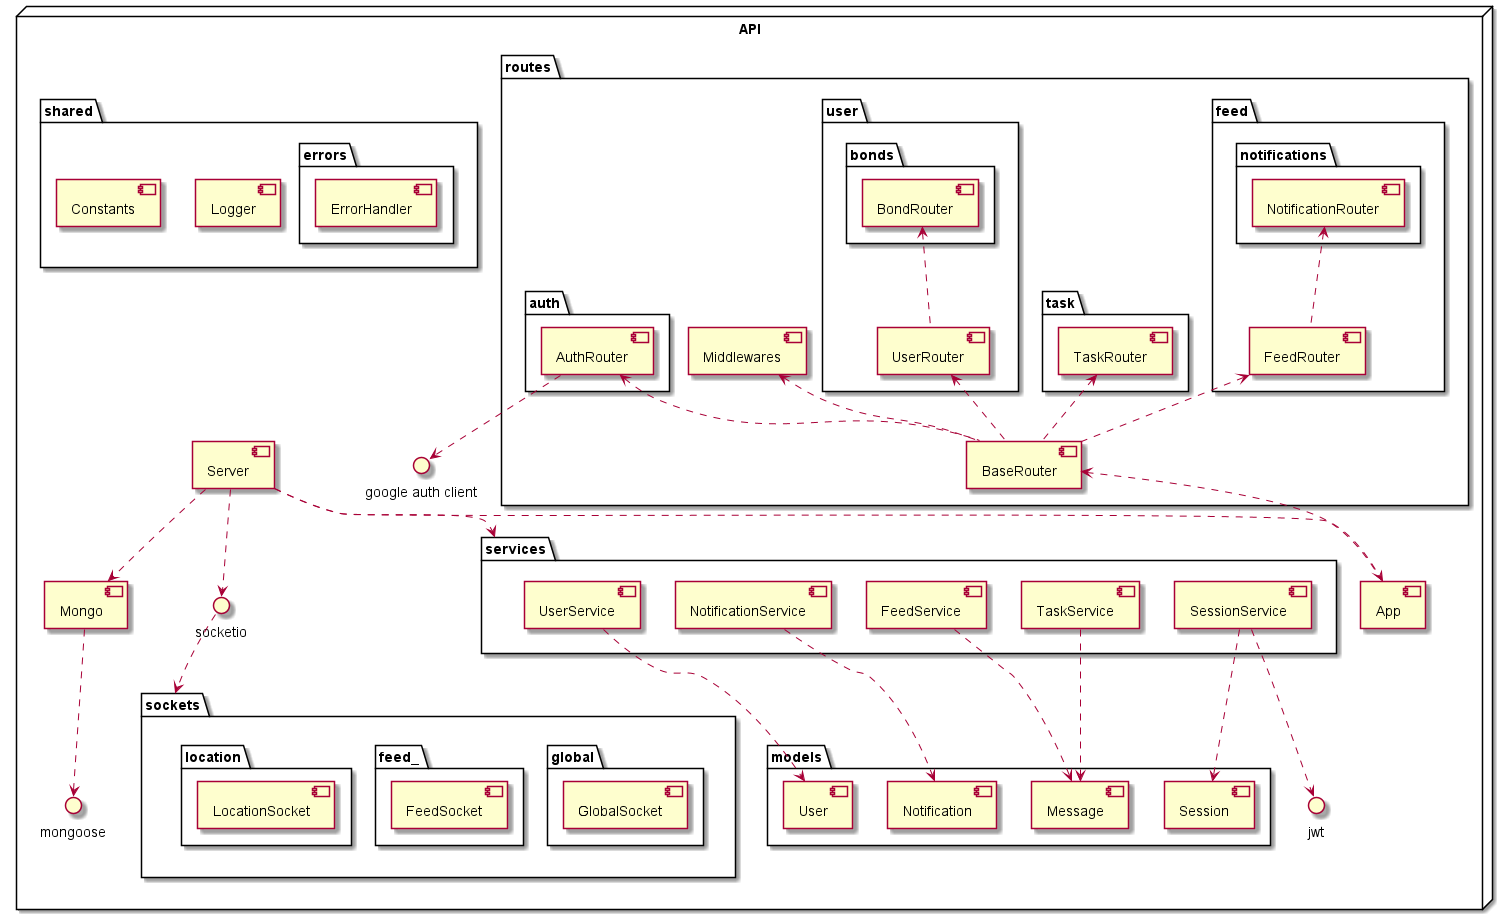
\includegraphics[width=1\textwidth]{images/Diseño/DiagramaPaquetesApi.png}
    \caption{Diagrama de paquetes de la API}
    \label{fig:diagrama_paquetes_api}
\end{figure}

Los paquetes \textbf{services} y \textbf{models} contienen toda la lógica de datos del sistema y son accedidos por las entidades de los dos paquetes mencionados con anterioridad. Las entidades del modelo de datos (ver \fref{ch:modelo_datos}) están en el paquete \textbf{models} mientras que los servicios que gestionan la persistencia y recuperación de dichas entidades están en \textbf{services}. Por último, en el paquete \textbf{shared} se encuentran funciones, datos y entidades comunes a todos los componentes del sistema como los errores, las cadenas de texto o el registro del sistema.

\subsection{Aplicación móvil}

Como se puede ver en la \fref{fig:diagrama_paquetes_app}, la aplicación móvil tiene un diagrama de paquetes que sigue la arquitectura de capas del \acrlong{mvvm} que ya planteamos en la fase de análisis en la \fref{sec:subsistema_app}. La parte clave es el paquete de \textbf{ui}, que se encuentra dividido a su vez en paquetes relativos a las distintas pantallas que tendrá la aplicación móvil, conteniendo la actividad, el modelo de la vista y cualquier otra pantalla, diálogo o fragmento auxiliar de la misma.

La interfaz de usuario se comunicará con los los repositorios del paquete \textbf{repositories} por medio de los objetos de valor (o \emph{value objects}) que se definirán en el paquete \textbf{vo}. Por último, la capa más profunda de la aplicación es aquella que se conectará con las \acrshort{api}, lo que da nombre al paquete en el que se albergan \textbf{api}. Este paquete expondrá una interfaz para el manejo del WebSocket y una factoría para los servicios del paquete \textbf{services}.

\begin{figure}[H]
    \centering
    \makebox[\textwidth][c]{
        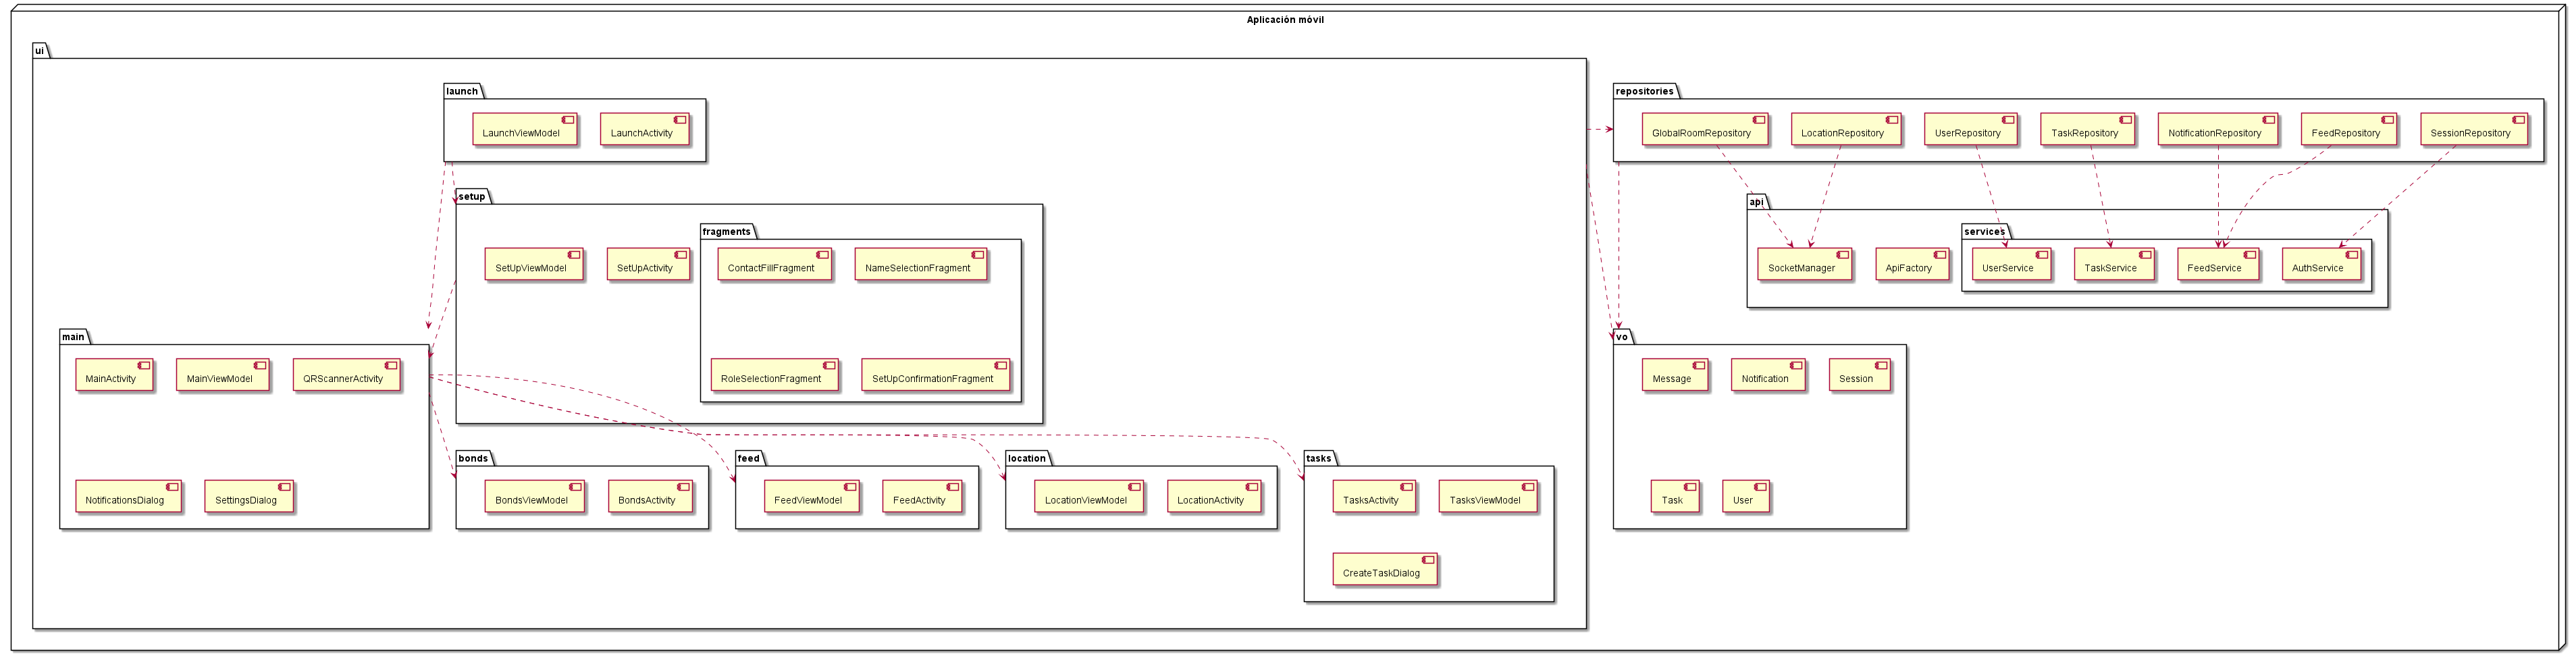
\includegraphics[width=1.1\textwidth]{images/Diseño/DiagramaPaquetesApp.png}
    }
    \caption{Diagrama de paquetes de la aplicación móvil}
    \label{fig:diagrama_paquetes_app}
\end{figure}

\section{Diagrama de despliegue}

La aplicación móvil se instalará en los dispositivos Android de los usuarios por medio de la \acrshort{apk} o el \acrlong{aab} de la aplicación. La \acrshort{api} se desplegará en una instancia AppService de Microsoft Azure como la que se especificó en el \fref{sec:despliegue_api}. La base de datos estará hospedada en el servicio en la nube de MongoDB, MongoDB Atlas. Las aplicaciones de los clientes se comunicarán con la \acrshort{api} por medio de peticiones \acrshort{http} \acrshort{rest} o de eventos a través del WebSocket. La \acrshort{api}, por su parte, se comunicará por red con la base de datos. Esto todo puede visualizarse en la \fref{fig:diagrama_despliegue}.

\begin{figure}[H]
    \centering
    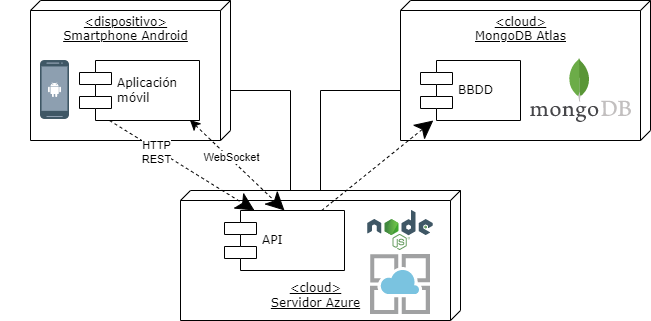
\includegraphics[width=0.65\textwidth]{images/Diseño/DiagramaDespliegue.drawio.png}
    \caption{Diagrama de despliegue del sistema}
    \label{fig:diagrama_despliegue}
\end{figure}

\begin{figure}[H]
    \centering
    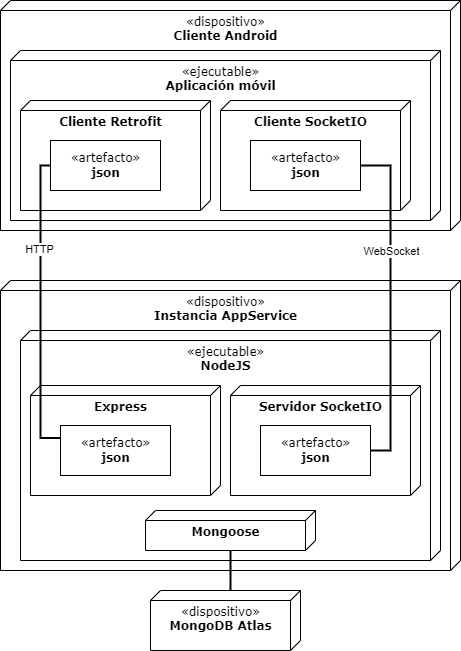
\includegraphics[width=0.6\textwidth]{images/Diseño/DiagramaComponentes.drawio.png}
    \caption{Diagrama de componentes del sistema}
    \label{fig:diagrama_componentes}
\end{figure}

\section{Diagrama de componentes}

El sistema estará compuesto por tres componentes principales análogos a las entidades de la sección anterior. Por un lado estará el \textbf{cliente}, que será el dispositivo del usuario y sobre el que se ejecutará la aplicación móvil; por otro lado estará la \textbf{API} ejecutada sobre una instancia de AppService; y por último, la \textbf{base de datos} alojada en MongoDB Atlas. En la aplicación habrá un cliente \acrshort{http} y otro cliente Socket.io (\fref{lib:api:socket_io}) que se comunicarán con los componentes Express (\fref{lib:api:express}) y servidor Socket.io de la \acrshort{api}, respectivamente. La comunicación definitiva entre la \acrshort{api} y la base de datos se llevará a cabo con el componente Mongoose (\fref{lib:api:mongoose}). Véase \fref{fig:diagrama_componentes}.
                 
\chapter{Diseño de clases}
\label{ch:diseño_clases}

\section{Clases de la API}

\begin{figure}[H]
    \centering
    \makebox[\textwidth][c]{
        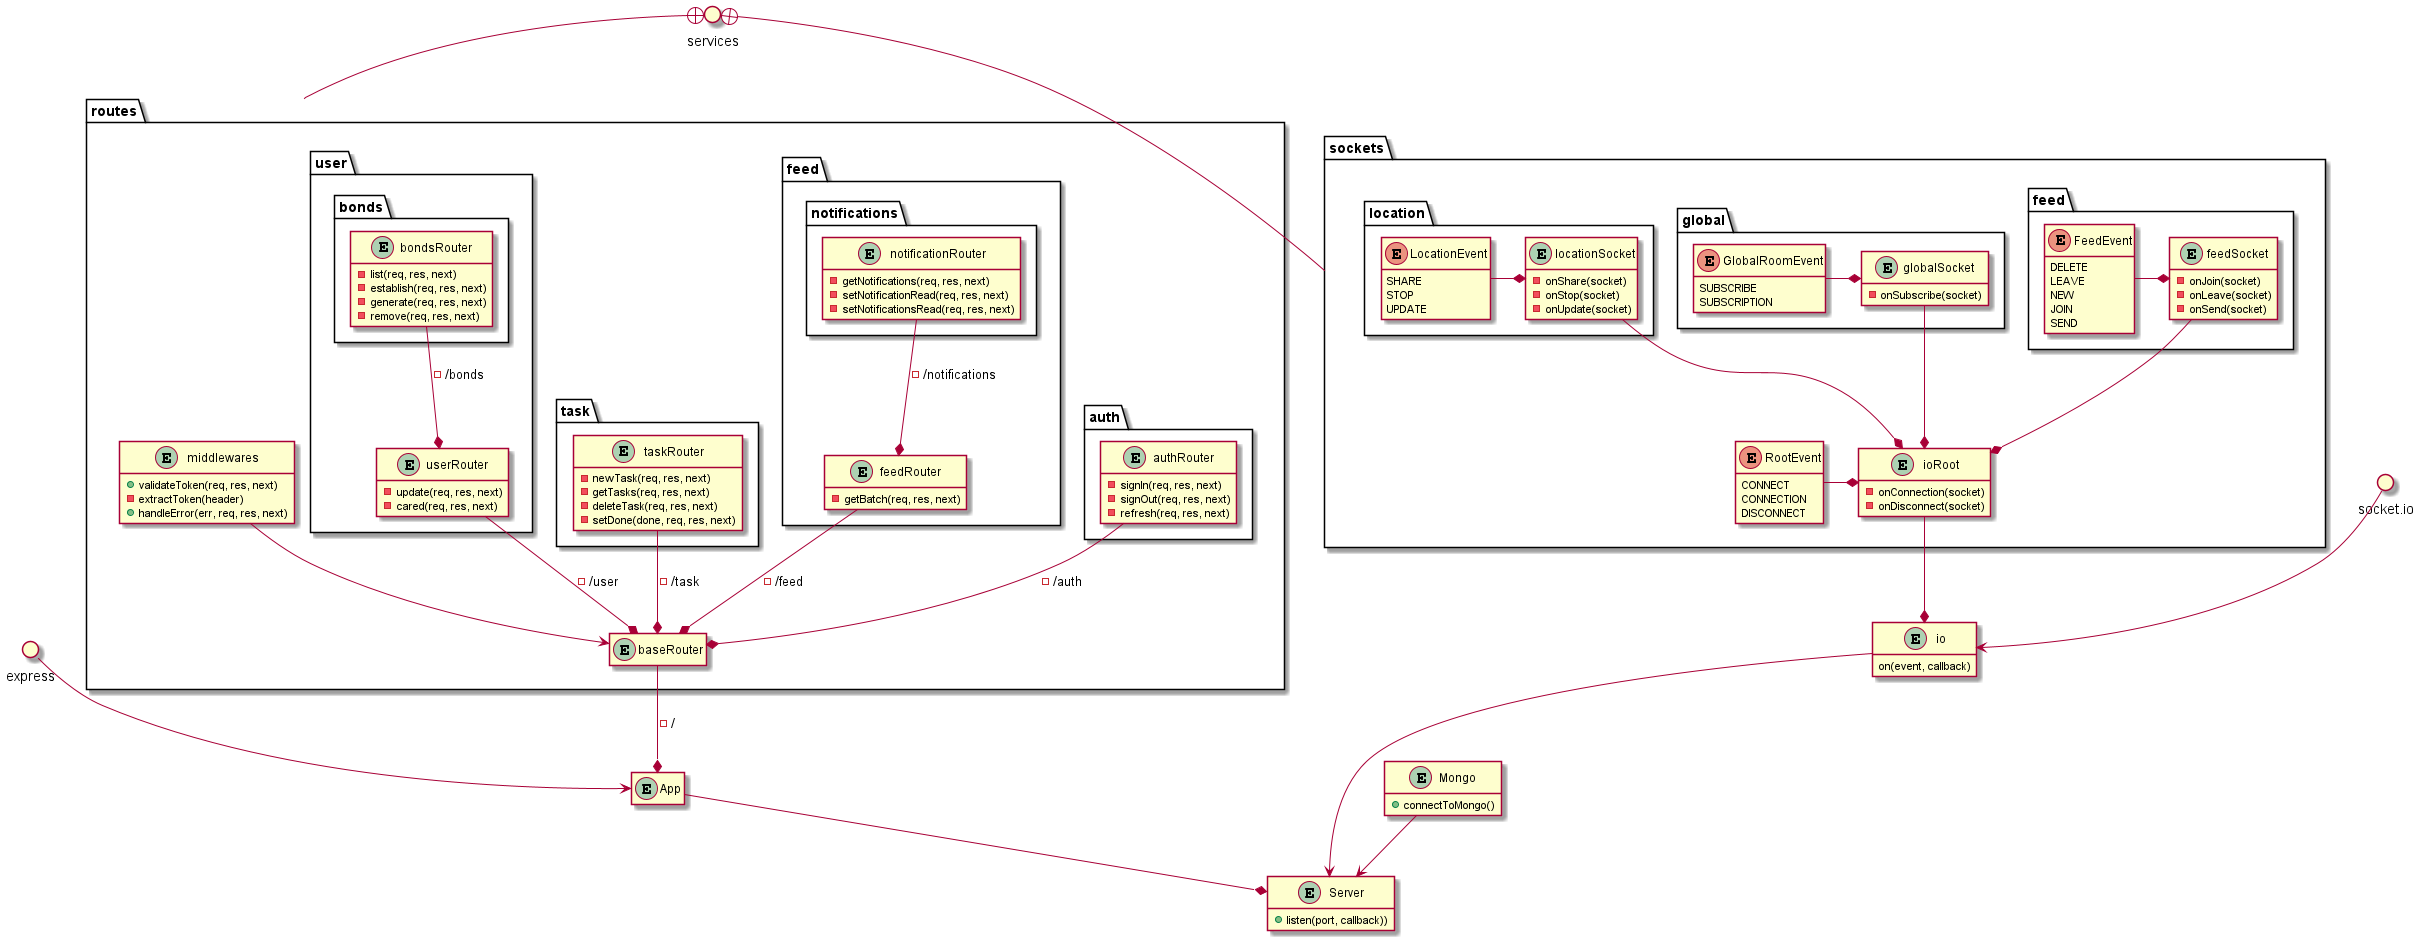
\includegraphics[width=1.2\textwidth]{images/Diseño/ClasesApiA.png}
    }
    \caption{Primera parte del diagrama de clases de la API}
    \label{fig:diagrama_clases_api_a}
\end{figure}

\begin{figure}[H]
    \centering
    \makebox[\textwidth][c]{
        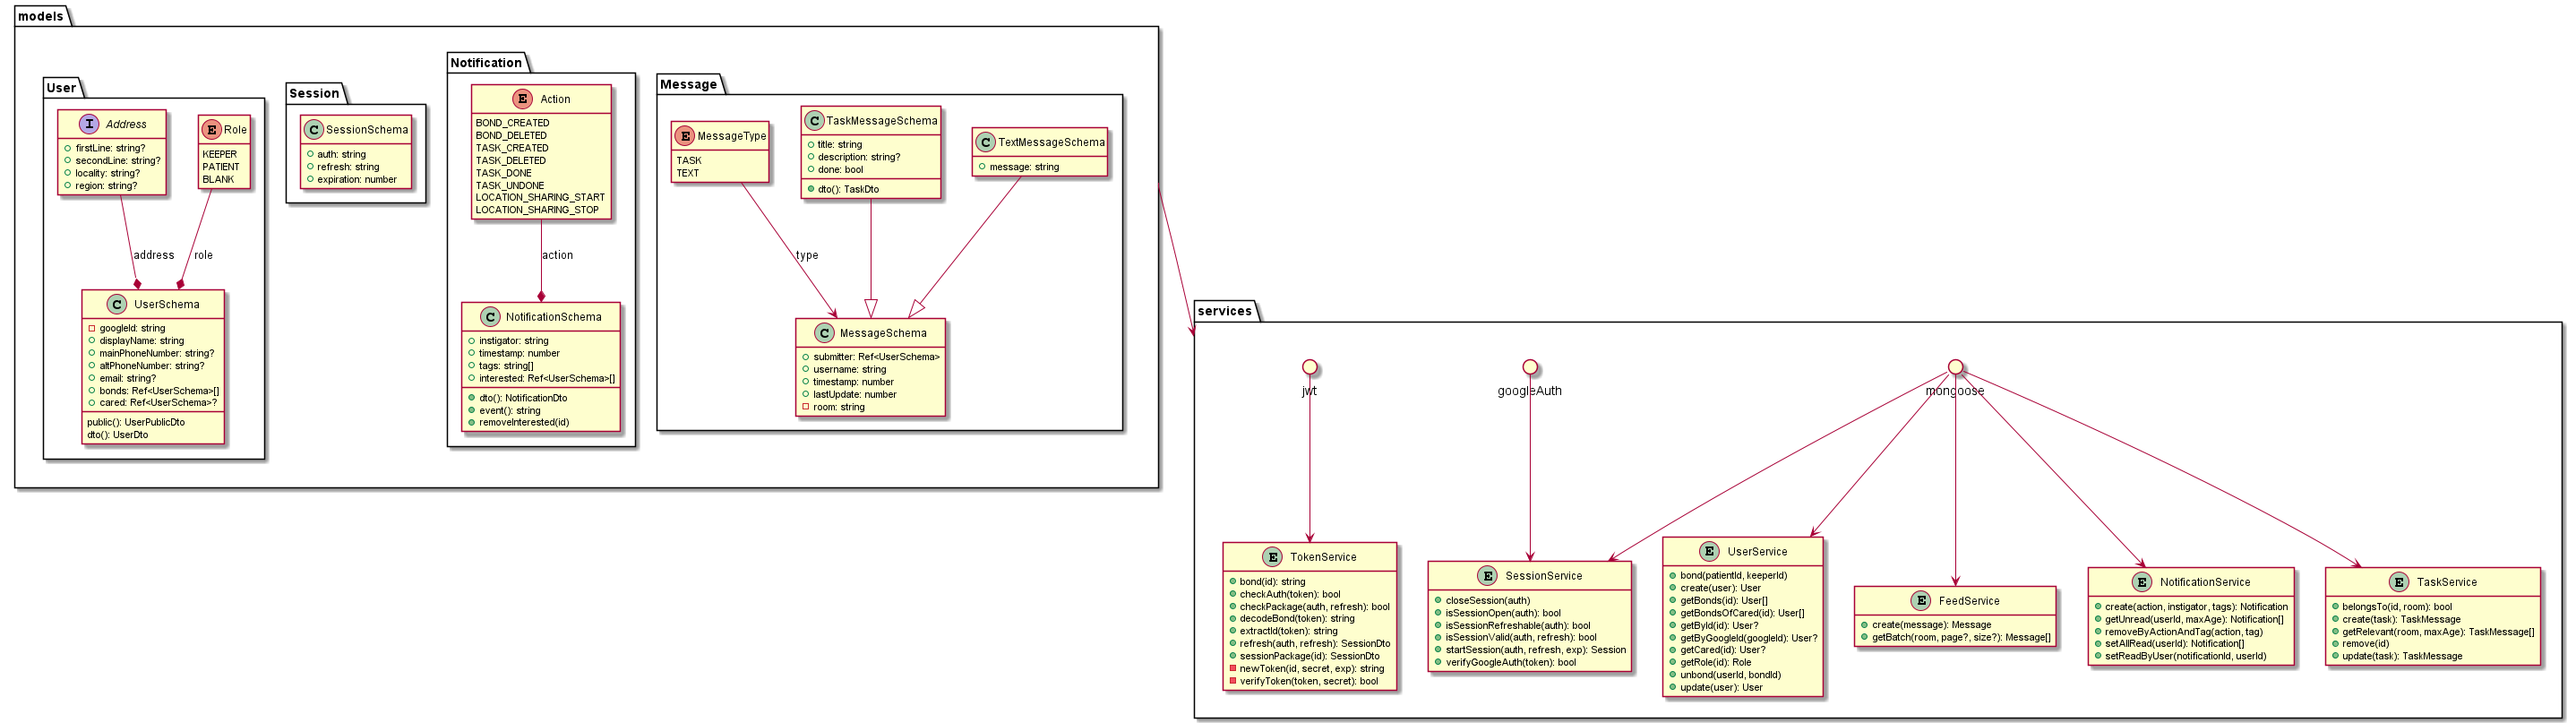
\includegraphics[width=1.2\textwidth]{images/Diseño/ClasesApiB.png}
    }
    \caption{Segunda parte del diagrama de clases de la API}
    \label{fig:diagrama_clases_api_b}
\end{figure}

\begin{figure}[H]
    \centering
    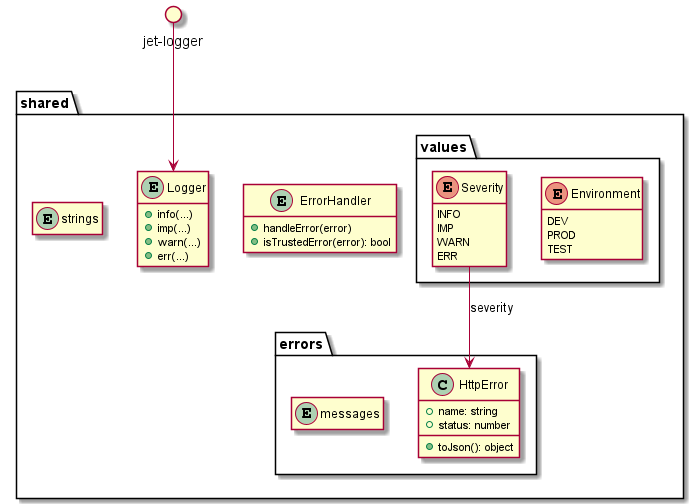
\includegraphics[width=0.3\textwidth]{images/Diseño/ClasesApiC.png}
    \caption{Tercera parte del diagrama de clases de la API}
    \label{fig:diagrama_clases_api_c}
\end{figure}

\subsection{Root}

\begin{longtable}{|p{0.25\textwidth} p{0.75\textwidth}|}
    \hline
    \multicolumn{2}{|l|}{\textbf{Server}} \\ \hline \hline
    Descripción      & Módulo principal del sistema. Inicializa todos los sistemas de la API en su lanzamiento desde el punto de entrada de la aplicación \\ \hline
    \multicolumn{2}{|l|}{Funciones} \\
    \emph{listen}  & Despliega el servidor en la direcciones y puerto especificados  \\ \hline
    \caption{Documentación de la entidad Server}
    \label{dis:api:server}
\end{longtable}

\begin{longtable}{|p{0.25\textwidth} p{0.75\textwidth}|}
    \hline
    \multicolumn{2}{|l|}{\textbf{App}} \\ \hline \hline
    Descripción      & Implementación del servidor Express, punto de entrada REST \\ \hline
    \caption{Documentación de la entidad App}
    \label{dis:api:app}
\end{longtable}

\begin{longtable}{|p{0.25\textwidth} p{0.75\textwidth}|}
    \hline
    \multicolumn{2}{|l|}{\textbf{Mongo}} \\ \hline \hline
    Descripción      & Módulo a cargo de la lógica relativa a la conexión de Mongoose con la base de datos \\ \hline
    \multicolumn{2}{|l|}{Funciones} \\
    \emph{connectToMongo}  & Crea la conexión con la base de datos remota  \\ \hline
    \caption{Documentación de la entidad Mongo}
    \label{dis:api:mongo}
\end{longtable}

\begin{longtable}{|p{0.25\textwidth} p{0.75\textwidth}|}
    \hline
    \multicolumn{2}{|l|}{\textbf{io}} \\ \hline \hline
    Descripción      & Implementación del servidor SocketIO, punto de entrada de los eventos WebSocket \\ \hline
    \multicolumn{2}{|l|}{Funciones} \\
    \emph{on}  & Define un evento y la función a realizar en el mismo  \\ \hline
    \caption{Documentación de la entidad io}
    \label{dis:api:io}
\end{longtable}

\subsection{Routes}

\begin{longtable}{|p{0.25\textwidth} p{0.75\textwidth}|}
    \hline
    \multicolumn{2}{|l|}{\textbf{baseRouter}} \\ \hline \hline
    Descripción      & Manejador raíz encargado de redireccionar las peticiones REST al manejador encargado de cada una según la ruta \\ \hline
    \caption{Documentación de la entidad baseRouter}
    \label{dis:api:base_router}
\end{longtable}

\begin{longtable}{|p{0.25\textwidth} p{0.75\textwidth}|}
    \hline
    \multicolumn{2}{|l|}{\textbf{authRouter}} \\ \hline \hline
    Descripción      & Manejador de las peticiones de /auth \\ \hline
    \multicolumn{2}{|l|}{Funciones} \\
    \emph{signIn}  & Crea una sesión para el usuario  \\ 
    \emph{signOut}  & Cierra la sesión de un usuario  \\ 
    \emph{refresh}  & Refresca la sesión del usuario  \\ \hline
    \caption{Documentación de la entidad authRouter}
    \label{dis:api:auth_router}
\end{longtable}

\begin{longtable}{|p{0.25\textwidth} p{0.75\textwidth}|}
    \hline
    \multicolumn{2}{|l|}{\textbf{feedRouter}} \\ \hline \hline
    Descripción      & Manejador de las peticiones de /feed \\ \hline
    \multicolumn{2}{|l|}{Funciones} \\
    \emph{getBatch}  & Devuelve el conjunto de mensajes solicitado por el usuario  \\ \hline
    \caption{Documentación de la entidad feedRouter}
    \label{dis:api:feed_router}
\end{longtable}

\begin{longtable}{|p{0.25\textwidth} p{0.75\textwidth}|}
    \hline
    \multicolumn{2}{|l|}{\textbf{notificationRouter}} \\ \hline \hline
    Descripción      & Manejador de las peticiones de /feed/notifications \\ \hline
    \multicolumn{2}{|l|}{Funciones} \\
    \emph{getNotifications}  & Devuelve las notificaciones pendientes del usuario  \\ 
    \emph{setNotificationRead}  & Marcar una notificación como leída  \\ 
    \emph{setNotificationsRead}  & Marca todas las notificaciones del usuario como leídas  \\ \hline
    \caption{Documentación de la entidad notificationRouter}
    \label{dis:api:notification_router}
\end{longtable}

\begin{longtable}{|p{0.25\textwidth} p{0.75\textwidth}|}
    \hline
    \multicolumn{2}{|l|}{\textbf{taskRouter}} \\ \hline \hline
    Descripción      & Manejador de las peticiones de /task \\ \hline
    \multicolumn{2}{|l|}{Funciones} \\
    \emph{newTask}  & Crea una nueva tarea  \\ 
    \emph{deleteTask}  & Elimina la tarea especificada  \\ 
    \emph{getTasks}  & Retorna las tareas relevantes relacionadas con el usuario  \\ 
    \emph{setTaskDone}  & Marca una tarea como hecha/no hecha  \\ \hline
    \caption{Documentación de la entidad taskRouter}
    \label{dis:api:task_router}
\end{longtable}

\begin{figure}[H]
\begin{longtable}{|p{0.25\textwidth} p{0.75\textwidth}|}
    \hline
    \multicolumn{2}{|l|}{\textbf{userRouter}} \\ \hline \hline
    Descripción      & Manejador de las peticiones de /user \\ \hline
    \multicolumn{2}{|l|}{Funciones} \\
    \emph{cared}  & Devuelve la información del paciente vinculado con el usuario  \\
    \emph{update}  & Actualiza la información del usuario  \\  \hline
    \caption{Documentación de la entidad userRouter}
    \label{dis:api:user_router}
\end{longtable}
\end{figure}

\begin{longtable}{|p{0.25\textwidth} p{0.75\textwidth}|}
    \hline
    \multicolumn{2}{|l|}{\textbf{bondsRouter}} \\ \hline \hline
    Descripción      & Manejador de las peticiones de /user/bonds \\ \hline
    \multicolumn{2}{|l|}{Funciones} \\
    \emph{list}  & Devuelve los vínculos del usuario  \\
    \emph{establish}  & Crea un vínculo entre usuarios  \\
    \emph{generate}  & Genera un código de vinculación  \\
    \emph{remove} & Elimina un vínculo entre usuarios \\ \hline
    \caption{Documentación de la entidad bondsRouter}
    \label{dis:api:bonds_router}
\end{longtable}

\subsection{Sockets}

\begin{longtable}{|p{0.25\textwidth} p{0.75\textwidth}|}
    \hline
    \multicolumn{2}{|l|}{\textbf{ioRoot}} \\ \hline \hline
    Descripción      & Manejador raíz encargado de los eventos de conexión y desconexión y de gestionar el registro de manejadores \\ \hline
    \caption{Documentación de la entidad ioRoot}
    \label{dis:api:io_root}
\end{longtable}

\begin{longtable}{|p{0.25\textwidth} p{0.75\textwidth}|}
    \hline
    \multicolumn{2}{|l|}{\textbf{RootEvent}} \\ \hline \hline
    Descripción      & Eventos de conexión al socket \\ \hline
    \multicolumn{2}{|l|}{Valores} \\
    \emph{CONNECT}  & Intento de conexión al socket  \\
    \emph{CONNECTION}  & Conexión exitosa al socket  \\
    \emph{DISCONNECT}  & Desconexión del socket \\ \hline
    \caption{Documentación del enumerado RootEvent}
    \label{dis:api:root_event}
\end{longtable}

\hspace{\textwidth}
\begin{longtable}{|p{0.25\textwidth} p{0.75\textwidth}|}
    \hline
    \multicolumn{2}{|l|}{\textbf{feedSocket}} \\ \hline \hline
    Descripción      & Manejador de la sala del Feed \\ \hline
    \multicolumn{2}{|l|}{Funciones} \\
    \emph{onJoin}  & Gestiona la entrada de un usuario en la sala  \\
    \emph{onLeave}  & Gestione el abandono de la sala de un usuario  \\
    \emph{onSend}  & Maneja el envío de un mensaje  \\ \hline
    \caption{Documentación de la entidad feedSocket}
    \label{dis:api:feed_socket}
\end{longtable}

\begin{longtable}{|p{0.25\textwidth} p{0.75\textwidth}|}
    \hline
    \multicolumn{2}{|l|}{\textbf{FeedEvent}} \\ \hline \hline
    Descripción      & Eventos de la sala del feed \\ \hline
    \multicolumn{2}{|l|}{Valores} \\
    \emph{DELETE}  & Eliminación de un mensaje  \\
    \emph{LEAVE}  & Abandono de la sala  \\
    \emph{NEW}  & Nuevo usuario en la sala  \\
    \emph{JOIN}  & Unión a la sala  \\
    \emph{SEND}  & Envío de un nuevo mensaje  \\ \hline
    \caption{Documentación del enumerado FeedEvent de la API}
    \label{dis:api:feed_event}
\end{longtable}

\begin{longtable}{|p{0.25\textwidth} p{0.75\textwidth}|}
    \hline
    \multicolumn{2}{|l|}{\textbf{globalSocket}} \\ \hline \hline
    Descripción      & Manejador de la sala Global \\ \hline
    \multicolumn{2}{|l|}{Funciones} \\
    \emph{onSubscribe}  & Gestiona la suscripción de un usuario a la sala \\ \hline
    \caption{Documentación de la entidad globalSocket}
    \label{dis:api:global_socket}
\end{longtable}

\begin{longtable}{|p{0.25\textwidth} p{0.75\textwidth}|}
    \hline
    \multicolumn{2}{|l|}{\textbf{GlobalEvent}} \\ \hline \hline
    Descripción      & Eventos de la sala global \\ \hline
    \multicolumn{2}{|l|}{Valores} \\
    \emph{SUBSCRIBE}  & Unión a la sala  \\
    \emph{SUBSCRIPTION} & Nuevo usuario en la sala  \\ \hline
    \caption{Documentación del enumerado GlobalEvent de la API}
    \label{dis:api:global_event}
\end{longtable}

\hspace{\textwidth}
\begin{longtable}{|p{0.25\textwidth} p{0.75\textwidth}|}
    \hline
    \multicolumn{2}{|l|}{\textbf{locationSocket}} \\ \hline \hline
    Descripción      & Manejador de la sala de la geolocalización \\ \hline
    \multicolumn{2}{|l|}{Funciones} \\
    \emph{onShare}  & Gestiona la entrada de un usuario en la sala  \\
    \emph{onStop}  & Gestione el abandono de la sala de un usuario  \\
    \emph{onUpdate}  & Maneja el envío de una localización  \\ \hline
    \caption{Documentación de la entidad locationSocket}
    \label{dis:api:location_socket}
\end{longtable}

\vspace{-15pt}
\begin{longtable}{|p{0.25\textwidth} p{0.75\textwidth}|}
    \hline
    \multicolumn{2}{|l|}{\textbf{LocationEvent}} \\ \hline \hline
    Descripción      & Eventos de la sala Location \\ \hline
    \multicolumn{2}{|l|}{Valores} \\
    \emph{SHARE}  & Unión a la sala  \\
    \emph{STOP} & Abandono de la sala  \\
    \emph{UPDATE} & Envío de una nueva ubicación  \\ \hline
    \caption{Documentación del enumerado LocationEvent de la API}
    \label{dis:api:location_event}
\end{longtable}

\vspace{-25pt}
\subsection{Services}

\begin{longtable}{|p{0.25\textwidth} p{0.75\textwidth}|}
    \hline
    \multicolumn{2}{|l|}{\textbf{FeedService}} \\ \hline \hline
    Descripción      & Servicio a cargo de los mensajes del feed \\ \hline
    \multicolumn{2}{|l|}{Funciones} \\
    \emph{create}  & Crea y persiste un nuevo mensaje  \\
    \emph{getBatch}  & Devuelve la lista de mensajes especificada  \\ \hline
    \caption{Documentación de la clase FeedService de la API}
    \label{dis:api:feed_service}
\end{longtable}

\vspace{-15pt}
\begin{longtable}{|p{0.3\textwidth} p{0.7\textwidth}|}
    \hline
    \multicolumn{2}{|l|}{\textbf{NotificationService}} \\ \hline \hline
    Descripción      & Servicio a cargo de las notificaciones \\ \hline
    \multicolumn{2}{|l|}{Funciones} \\
    \emph{create}  & Crea y persiste una nueva notificación  \\
    \emph{getUnread}  & Devuelve la lista de notificaciones no leídas de un usuario  \\
    \emph{removeByActionAndTag}  & Elimina las notificaciones que tienen la misma acción y etiquetas  \\
    \emph{setAllRead}  & Marca todas las notificaciones de un usuario como leídas  \\
    \emph{setReadByUser}  & Marca una notificación como leída  \\ \hline
    \caption{Documentación de la clase NotificationService}
    \label{dis:api:notification_service}
\end{longtable}

\begin{longtable}{|p{0.25\textwidth} p{0.75\textwidth}|}
    \hline
    \multicolumn{2}{|l|}{\textbf{SessionService}} \\ \hline \hline
    Descripción      & Servicio a cargo de las sesiones de usuario \\ \hline
    \multicolumn{2}{|l|}{Funciones} \\
    \emph{closeSession}  & Cierra la sesión especificada  \\
    \emph{isSessionOpen}  & Comprueba si una sesión está activa  \\
    \emph{isSessionRefreshable}  & Comprueba si una sesión se puede refrescar  \\
    \emph{isSessionValid}  & Comprueba si una sesión es válida  \\
    \emph{startSession}  & Crea una nueva sesión de usuario  \\
    \emph{verifyGoogleAuth}  & Verifica un token de autenticación de Google  \\ \hline
    \caption{Documentación de la clase SessionService}
    \label{dis:api:session_service}
\end{longtable}

\vspace{-10pt}
\begin{longtable}{|p{0.25\textwidth} p{0.75\textwidth}|}
    \hline
    \multicolumn{2}{|l|}{\textbf{TaskService}} \\ \hline \hline
    Descripción      & Servicio a cargo de las tareas \\ \hline
    \multicolumn{2}{|l|}{Funciones} \\
    \emph{belongsTo}  & Comprueba si la tarea pertenece a un usuario  \\
    \emph{create}  & Crea y persiste una nueva tarea  \\
    \emph{getRelevant}  & Devuelve la lista de tareas relevantes de un usuario  \\
    \emph{remove}  & Elimina la tarea especificada  \\
    \emph{update}  & Actualiza una tarea  \\ \hline
    \caption{Documentación de la clase TaskService de la API}
    \label{dis:api:task_service}
\end{longtable}

\vspace{-10pt}
\begin{longtable}{|p{0.25\textwidth} p{0.75\textwidth}|}
    \hline
    \multicolumn{2}{|l|}{\textbf{TokenService}} \\ \hline \hline
    Descripción      & Servicio para proveer y gestionar tokens \\ \hline
    \multicolumn{2}{|l|}{Funciones} \\
    \emph{bond}  & Genera un token de vinculación  \\
    \emph{checkAuth}  & Comprueba la validez de un token de autenticación  \\
    \emph{checkPackage}  & Comprueba la validez de una dupla de tokens de sesión  \\
    \emph{decodeBond}  & Descodifica un token de vinculación  \\
    \emph{extractId}  & Devuelve la ID de usuario almacenada en un token  \\
    \emph{newToken}  & Produce un nuevo token según la ID de usuario, el secreto y el tiempo de expiración  \\
    \emph{refresh}  & Genera una nueva tupla de tokens de sesión a partir una válida \\
    \emph{session}  & Genera una tupla de tokens de sesión nueva  \\
    \emph{verifyToken}  & Verifica la validez de un token  \\ \hline
    \caption{Documentación de la clase TokenService}
    \label{dis:api:token_service}
\end{longtable}

\begin{longtable}{|p{0.25\textwidth} p{0.75\textwidth}|}
    \hline
    \multicolumn{2}{|l|}{\textbf{UserService}} \\ \hline \hline
    Descripción      & Servicio a cargo de los datos de usuario \\ \hline
    \multicolumn{2}{|l|}{Funciones} \\
    \emph{bond}  & Crea un vínculo entre usuarios  \\
    \emph{create}  & Crea un nuevo usuario \\
    \emph{getBonds}  & Devuelve los vínculos de un usuario  \\
    \emph{getBondsOfCared}  & Devuelve los vínculos del paciente vinculado  \\
    \emph{getById}  & Retorna el usuario con la identidad especificada  \\
    \emph{getByGoogleId}  & Retorna el usuario con la identidad de Google especificada  \\
    \emph{getCared}  & Devuelve el paciente vinculado de un usuario  \\
    \emph{getRole}  & Devuelve el rol de un usuario  \\
    \emph{unbond} & Elimina el vínculo entre dos usuarios \\
    \emph{update}  & Actualiza los datos de un usuario  \\ \hline
    \caption{Documentación de la clase UserService de la API}
    \label{dis:api:user_service}
\end{longtable}

\vspace{-30pt}
\subsection{Models}

\vspace{-10pt}
\begin{longtable}{|p{0.5\textwidth} p{0.5\textwidth}|}
    \hline
    \multicolumn{2}{|l|}{\textbf{Action}} \\ \hline \hline
    Descripción      & Accciones notificables \\ \hline
    \multicolumn{2}{|l|}{Valores} \\
    \emph{BOND\textunderscore CREATED}  & Creación de un vínculo  \\
    \emph{BOND\textunderscore DELETED}  & Eliminación de un vínculo  \\
    \emph{TASK\textunderscore CREATED}  & Creación de una tarea  \\
    \emph{TASK\textunderscore DELETED}  & Eliminación de una tarea  \\
    \emph{TASK\textunderscore DONE}  & Actualización de una tarea a hecha  \\
    \emph{TASK\textunderscore UNDONE}  & Actualización de una tarea a no hecha  \\
    \emph{LOCATION\textunderscore SHARING\textunderscore START}  & Ubicación empezando a ser compartida  \\
    \emph{LOCATION\textunderscore SHARING\textunderscore STOP}  & Ubicación dejando de ser compartida  \\ \hline
    \caption{Documentación del enumerado Action de la API}
    \label{dis:api:action}
\end{longtable}

\vspace{-20pt}
\begin{longtable}{|p{0.25\textwidth} p{0.75\textwidth}|}
    \hline
    \multicolumn{2}{|l|}{\textbf{Address}} \\ \hline \hline
    Descripción      & Abstracción de direcciones postales \\ \hline
    \multicolumn{2}{|l|}{Propiedades} \\
    \emph{firstLine}  & Primera línea (por ejemplo, calle y número)  \\
    \emph{secondLine}  & Segunda línea (por ejemplo, piso y puerta)  \\
    \emph{locality}  & Localidad  \\
    \emph{region}  & Región (por ejemplo, provincia o estado)  \\ \hline
    \caption{Documentación de la interfaz Address de la API}
    \label{dis:api:address}
\end{longtable}

\begin{longtable}{|p{0.25\textwidth} p{0.75\textwidth}|}
    \hline
    \multicolumn{2}{|l|}{\textbf{MessageType}} \\ \hline \hline
    Descripción      & Tipos de mensajes \\ \hline
    \multicolumn{2}{|l|}{Valores} \\
    \emph{TASK}  & Tarea  \\
    \emph{TEXT}  & Mensaje de texto  \\ \hline
    \caption{Documentación del enumerado MessageType de la API}
    \label{dis:api:message_type}
\end{longtable}

\begin{longtable}{|p{0.25\textwidth} p{0.75\textwidth}|}
    \hline
    \multicolumn{2}{|l|}{\textbf{MessageSchema}} \\ \hline \hline
    Descripción      & Esquema base de los mensajes \\ \hline
    \multicolumn{2}{|l|}{Propiedades} \\
    \emph{submitter}  & Referencia a la entidad del autor  \\
    \emph{username}  & Nombre del autor \\
    \emph{timestamp}  & Instante de envío \\
    \emph{lastUpdate}  & Última actualización  \\
    \emph{room}  & Sala de envío  \\ \hline
    \caption{Documentación del esquema de Message de la API}
    \label{dis:api:message}
\end{longtable}

\begin{longtable}{|p{0.25\textwidth} p{0.75\textwidth}|}
    \hline
    \multicolumn{2}{|l|}{\textbf{NotificationSchema}} \\ \hline \hline
    Descripción      & Esquema de las notificaciones de la aplicación \\ \hline
    \multicolumn{2}{|l|}{Propiedades} \\
    \emph{action}  & Acción a notificar  \\
    \emph{instigator}  & Autor de la acción  \\
    \emph{timestamp}  & Instante de realización de la acción  \\
    \emph{tags}  & Etiquetas con información extra de la notificación  \\
    \emph{interested}  & Lista de usuarios receptores de la notificación  \\ \hline
    \multicolumn{2}{|l|}{Funciones} \\
    \emph{dto}  & Devuelve un NotificationDto de la notificación  \\
    \emph{event}  & Devuelve el código de evento del WebSocket \\
    \emph{removeInterested}  & Elimina al usuario especificado de la lista de interesados  \\ \hline
    \caption{Documentación del esquema de Notification de la API}
    \label{dis:api:notification}
\end{longtable}

\newpage
\begin{longtable}{|p{0.25\textwidth} p{0.75\textwidth}|}
    \hline
    \multicolumn{2}{|l|}{\textbf{Role}} \\ \hline \hline
    Descripción      & Roles de los usuarios \\ \hline
    \multicolumn{2}{|l|}{Valores} \\
    \emph{PATIENT}  & Pacientes  \\
    \emph{KEEPER}  & Cuidadores  \\
    \emph{BLANK}  & Sin rol  \\ \hline
    \caption{Documentación del enumerado Role de la API}
    \label{dis:api:role}
\end{longtable}

\begin{longtable}{|p{0.25\textwidth} p{0.75\textwidth}|}
    \hline
    \multicolumn{2}{|l|}{\textbf{SessionSchema}} \\ \hline \hline
    Descripción      & Esquema de una sesión de usuario \\ \hline
    \multicolumn{2}{|l|}{Propiedades} \\
    \emph{auth}  & Token de autenticación de la sesión  \\
    \emph{refresh}  & Token de refresco de la sesión  \\
    \emph{expiration}  & Instante de expiración de la sesión  \\ \hline
    \caption{Documentación del esquema de Session de la API}
    \label{dis:api:session}
\end{longtable}

\begin{longtable}{|p{0.25\textwidth} p{0.75\textwidth}|}
    \hline
    \multicolumn{2}{|l|}{\textbf{TaskMessageSchema}} \\ \hline \hline
    Descripción      & Esquema de una tarea \\ \hline
    \multicolumn{2}{|l|}{Propiedades} \\
    \emph{title}  & Título  \\
    \emph{description}  & Descripción  \\
    \emph{done}  & Estado: hecha/no hecha  \\ \hline
    \multicolumn{2}{|l|}{Funciones} \\
    \emph{dto}  & Devuelve un TaskDto de la tarea  \\ \hline
    \caption{Documentación del esquema de TaskMessage de la API}
    \label{dis:api:task_message}
\end{longtable}

\begin{longtable}{|p{0.25\textwidth} p{0.75\textwidth}|}
    \hline
    \multicolumn{2}{|l|}{\textbf{TextMessageSchema}} \\ \hline \hline
    Descripción      & Esquema de los mensajes de texto del Feed \\ \hline
    \multicolumn{2}{|l|}{Propiedades} \\
    \emph{message}  & Mensaje enviado  \\ \hline
    \caption{Documentación del esquema de TextMessage de la API}
    \label{dis:api:text_message}
\end{longtable}

\begin{longtable}{|p{0.25\textwidth} p{0.75\textwidth}|}
    \hline
    \multicolumn{2}{|l|}{\textbf{UserSchema}} \\ \hline \hline
    Descripción      & Esquema de los usuarios de la aplicación \\ \hline
    \multicolumn{2}{|l|}{Propiedades} \\
    \emph{role}  & Rol  \\
    \emph{googleId}  & Identidad de Google  \\
    \emph{displayName}  & Nombre para mostrar al resto de usuarios  \\
    \emph{mainPhoneNumber}  & Teléfono principal  \\
    \emph{altPhoneNumber}  & Teléfono alternativo  \\
    \emph{address}  & Dirección postal  \\
    \emph{email}  & Dirección electrónica  \\
    \emph{bonds}  & Lista de usuarios vinculados de los pacientes  \\
    \emph{cared}  & Usuario vinculado de los cuidadores  \\ \hline
    \caption{Documentación del esquema de User de la API}
    \label{dis:api:user}
\end{longtable}

\subsection{Shared}

\begin{longtable}{|p{0.25\textwidth} p{0.75\textwidth}|}
    \hline
    \multicolumn{2}{|l|}{\textbf{Logger}} \\ \hline \hline
    Descripción      & Encapsulación de la lógica del registro  \\ \hline
    \multicolumn{2}{|l|}{Funciones} \\
    \emph{info}  & Registra un mensaje de información  \\
    \emph{imp}  & Registra un mensaje importante  \\
    \emph{warn}  & Registra un mensaje de advertencia  \\
    \emph{err}  & Registra un mensaje de error  \\  \hline
    \caption{Documentación de la entidad Logger}
    \label{dis:api:logger}
\end{longtable}

\begin{longtable}{|p{0.25\textwidth} p{0.75\textwidth}|}
    \hline
    \multicolumn{2}{|l|}{\textbf{ErrorHandler}} \\ \hline \hline
    Descripción      & Manejador de errores  \\ \hline
    \multicolumn{2}{|l|}{Funciones} \\
    \emph{handleError}  & Gestiona y procesa un error  \\
    \emph{isTrustedError}  & Comprueba si es un error conocido  \\  \hline
    \caption{Documentación de la entidad ErrorHandler}
    \label{dis:api:error_handler}
\end{longtable}

\newpage
\begin{longtable}{|p{0.25\textwidth} p{0.75\textwidth}|}
    \hline
    \multicolumn{2}{|l|}{\textbf{HttpError}} \\ \hline \hline
    Descripción      & Errores con respuesta HTTP definida  \\ \hline
    \multicolumn{2}{|l|}{Propiedades} \\
    \emph{name}  & Nombre  \\
    \emph{severity}  & Severidad  \\
    \emph{status}  & Código de estado HTTP  \\ \hline
    \multicolumn{2}{|l|}{Funciones} \\
    \emph{toJson}  & Devuelve un JSON para enviar el error como respuesta  \\  \hline
    \caption{Documentación de la clase HttpError}
    \label{dis:api:http_error}
\end{longtable}

\begin{longtable}{|p{0.25\textwidth} p{0.75\textwidth}|}
    \hline
    \multicolumn{2}{|l|}{\textbf{Severity}} \\ \hline \hline
    Descripción      & Severidad \\ \hline
    \multicolumn{2}{|l|}{Valores} \\
    \emph{INFO}  & Información  \\
    \emph{IMP}  & Información importante  \\
    \emph{WARN}  & Advertencia  \\
    \emph{ERROR}  & Error severo  \\ \hline
    \caption{Documentación del enumerado Severity de la API}
    \label{dis:api:severity}
\end{longtable}

\begin{longtable}{|p{0.25\textwidth} p{0.75\textwidth}|}
    \hline
    \multicolumn{2}{|l|}{\textbf{Environment}} \\ \hline \hline
    Descripción      & Entornos de ejecución \\ \hline
    \multicolumn{2}{|l|}{Valores} \\
    \emph{DEV}  & Desarrollo  \\
    \emph{PROD}  & Producción  \\
    \emph{TEST}  & Pruebas  \\ \hline
    \caption{Documentación del enumerado Environment de la API}
    \label{dis:api:environment}
\end{longtable}
\section{Clases de la aplicación móvil}

\begin{figure}[H]
    \centering
    \makebox[\textwidth][c]{
        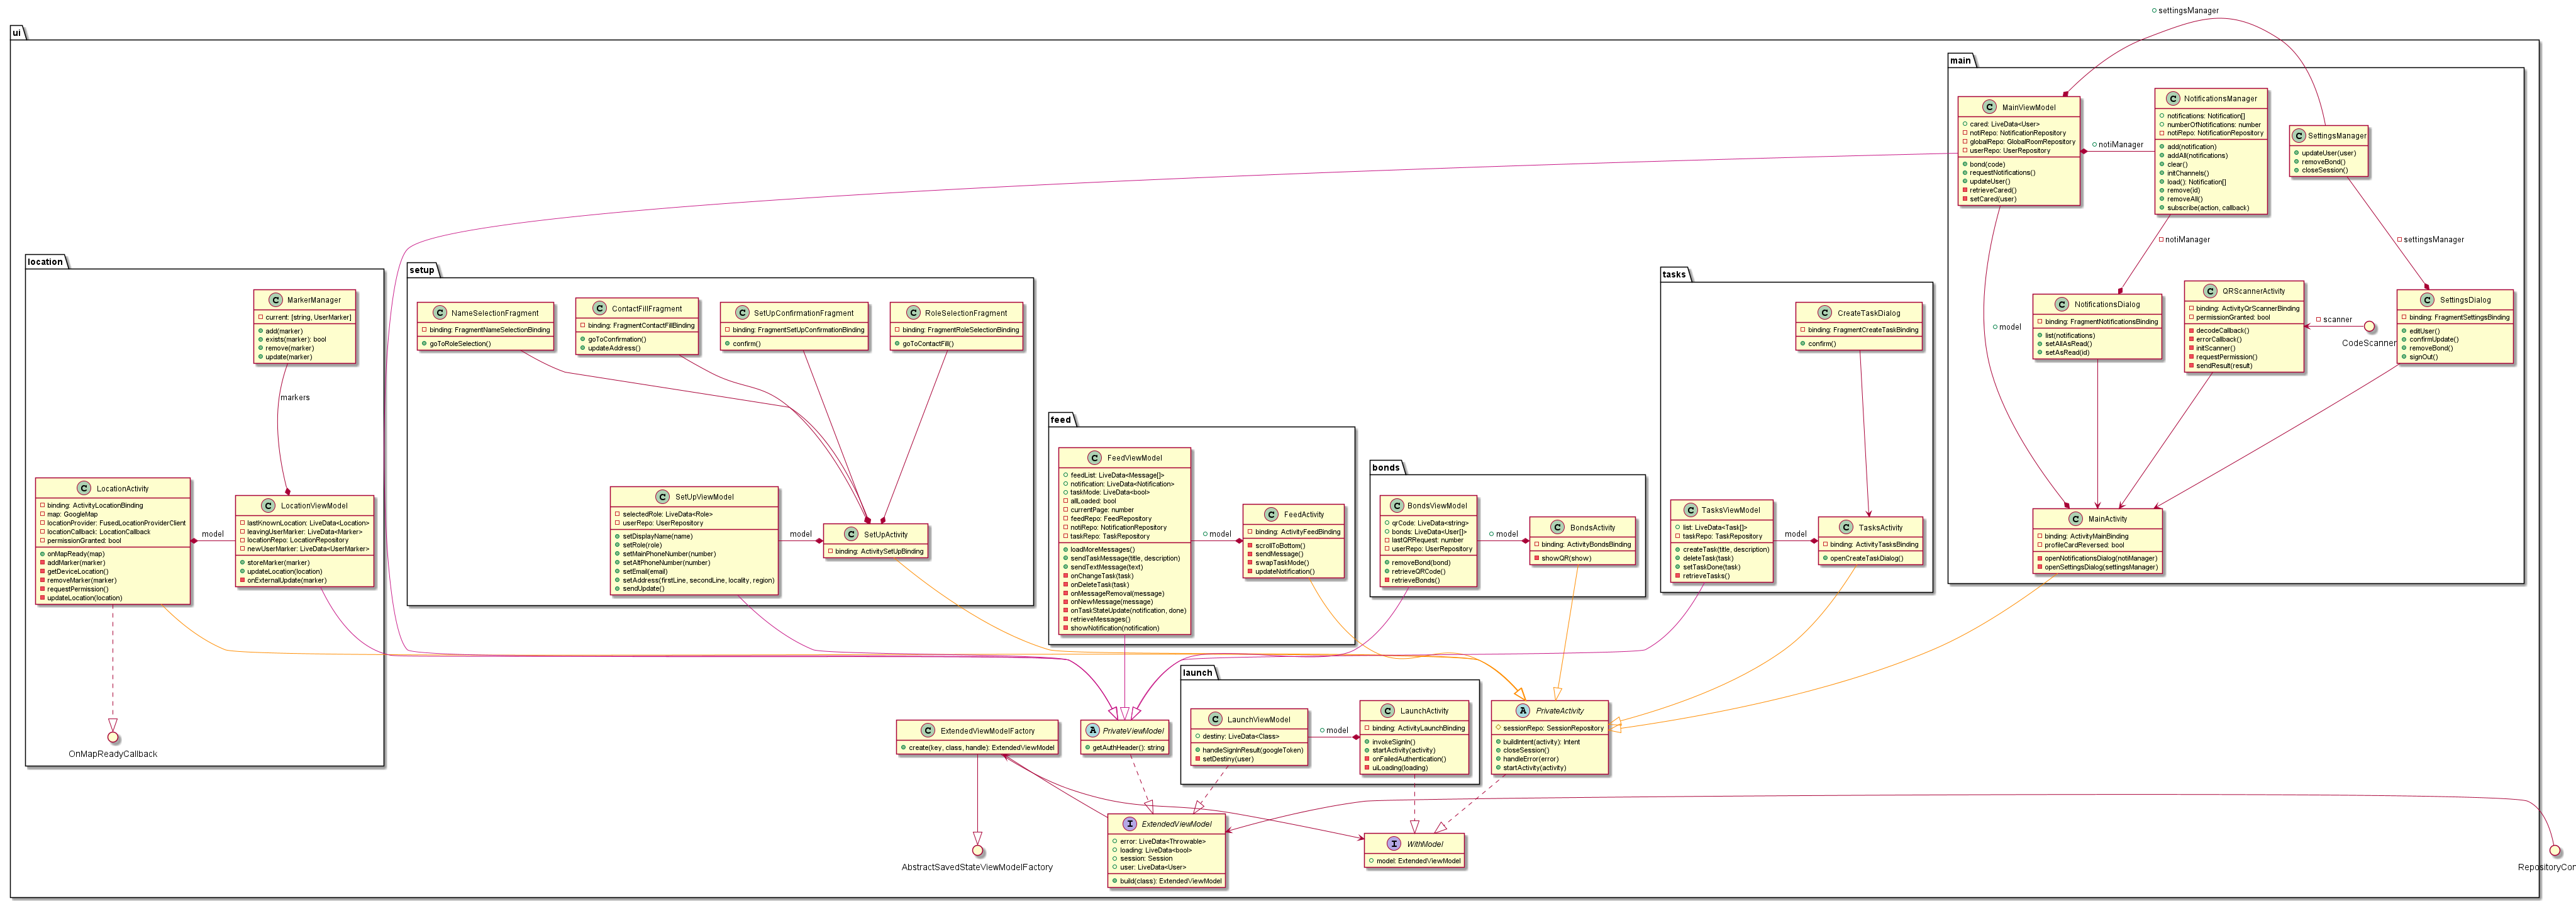
\includegraphics[width=1.3\textwidth]{images/Diseño/ClasesAppA.png}
    }
    \caption{Primera parte del diagrama de clases de la aplicación móvil}
    \label{fig:diagrama_clases_app_a}
\end{figure}

\begin{figure}[H]
    \centering
    \makebox[\textwidth][c]{
        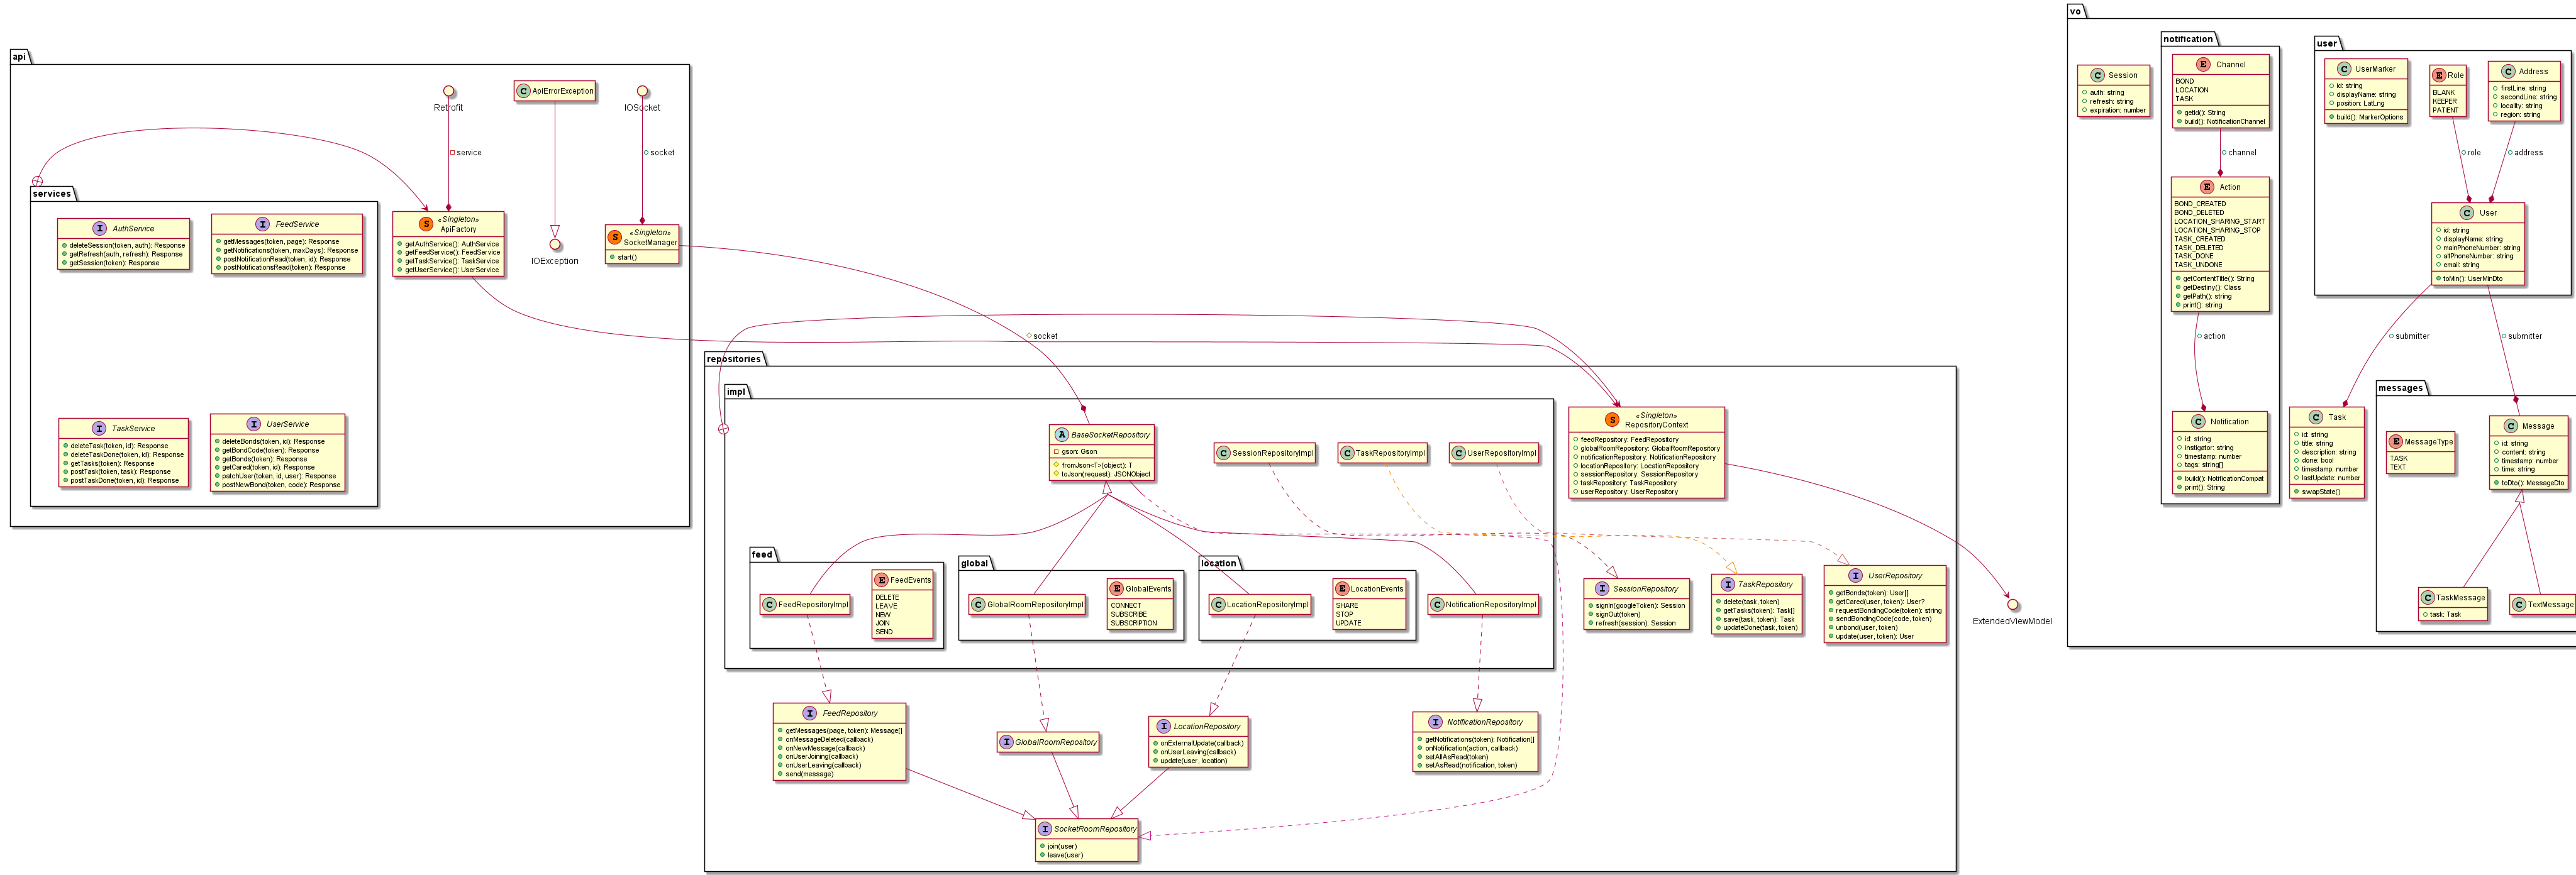
\includegraphics[width=1.3\textwidth]{images/Diseño/ClasesAppB.png}
    }
    \caption{Segunda parte del diagrama de clases de la aplicación móvil}
    \label{fig:diagrama_clases_app_b}
\end{figure}

\newpage
\subsection{UI}

\begin{longtable}{|p{0.25\textwidth} p{0.75\textwidth}|}
    \hline
    \multicolumn{2}{|l|}{\textbf{ExtendedViewModel}} \\ \hline \hline
    Descripción      & Interfaz común para los ViewModel a emplear en la aplicación \\ \hline
    \multicolumn{2}{|l|}{Propiedades} \\
    \emph{error}  & Contenedor del último error ocurrido  \\ 
    \emph{loading}  & Contenedor del estado de carga de la pantalla  \\ 
    \emph{session}  & Sesión actual \\ 
    \emph{user}  & Contenedor de los datos del usuario  \\ \hline
    \multicolumn{2}{|l|}{Funciones} \\
    \emph{build}  & Constructor para la creación en ExtendedViewModelFactory (\ref{dis:app:extended_viewmodel_factory})  \\ \hline
    \caption{Documentación de la interfaz ExtendedViewModel}
    \label{dis:app:extended_viewmodel}
\end{longtable}

\begin{longtable}{|p{0.25\textwidth} p{0.75\textwidth}|}
    \hline
    \multicolumn{2}{|l|}{\textbf{WithModel}} \\ \hline \hline
    Descripción      & Interfaz para clases que implementen un ExtendedViewModel (\ref{dis:app:extended_viewmodel}) \\ \hline
    \multicolumn{2}{|l|}{Propiedades} \\
    \emph{model}  & ExtendedViewModel implementado  \\ \hline
    \caption{Documentación de la interfaz WithModel}
    \label{dis:app:with_model}
\end{longtable}

\begin{longtable}{|p{0.25\textwidth} p{0.75\textwidth}|}
    \hline
    \multicolumn{2}{|l|}{\textbf{ExtendedViewModelFactory}} \\ \hline \hline
    Descripción      & Factoría de clases que implementan ExtendedViewModel (\ref{dis:app:extended_viewmodel}) \\ \hline
    \multicolumn{2}{|l|}{Funciones} \\
    \emph{create}  & Crea el ExtendedViewModel especificado  \\ \hline
    \caption{Documentación de la clase ExtendedViewModelFactory}
    \label{dis:app:extended_viewmodel_factory}
\end{longtable}

\begin{longtable}{|p{0.25\textwidth} p{0.75\textwidth}|}
    \hline
    \multicolumn{2}{|l|}{\textbf{PrivateViewModel}} \\ \hline \hline
    Descripción      & Implementación base de las clases ExtendedViewModel \\ \hline
    \multicolumn{2}{|l|}{Funciones} \\
    \emph{getAuthHeader}  & Obtiene y devuelve el encabezado de autenticación para las peticiones REST  \\ \hline
    \caption{Documentación de la clase PrivateViewModel}
    \label{dis:app:private_viewmodel}
\end{longtable}

\begin{longtable}{|p{0.25\textwidth} p{0.75\textwidth}|}
    \hline
    \multicolumn{2}{|l|}{\textbf{PrivateActivity}} \\ \hline \hline
    Descripción      & Implementación base de las actividades que implementen WithModel \\ \hline
    \multicolumn{2}{|l|}{Propiedades} \\
    \emph{sessionRepo}  & Repositorio para operaciones relacionadas con la sesión  \\ \hline
    \multicolumn{2}{|l|}{Funciones} \\
    \emph{buildIntent}  & Construye una intención de navegación a otra actividad con la información necesaria \\ 
    \emph{closeSession}  & Elimina los datos de sesión y retorna a LaunchActivity (\ref{dis:app:launch_activity}) \\
    \emph{handleError}  & Implementación por defecto para manejo de errores  \\ 
    \emph{startActivity}  & Inicia la actividad especificada  \\ \hline
    \caption{Documentación de la clase PrivateActivity}
    \label{dis:app:private_activity}
\end{longtable}

\vspace{-20pt}
\subsubsection{Launch}

\begin{longtable}{|p{0.3\textwidth} p{0.7\textwidth}|}
    \hline
    \multicolumn{2}{|l|}{\textbf{LaunchActivity}} \\ \hline \hline
    Descripción      & Actividad de inicio de la aplicación con el inicio de sesión \\ \hline
    \multicolumn{2}{|l|}{Propiedades} \\
    \emph{binding}  & Vista vinculada  \\
    \emph{model}  & Modelo de vista  \\ \hline
    \multicolumn{2}{|l|}{Funciones} \\
    \emph{invokeSign}  & Inicia el proceso de inicio de sesión  \\ 
    \emph{startActivity}  & Inicia la siguiente actividad  \\ 
    \emph{onFailedAuthentication}  & Gestiona errores de autenticación  \\ 
    \emph{uiLoading}  & Cambia el estado de carga de la interfaz  \\ \hline
    \caption{Documentación de la clase LaunchActivity}
    \label{dis:app:launch_activity}
\end{longtable}

\begin{longtable}{|p{0.25\textwidth} p{0.75\textwidth}|}
    \hline
    \multicolumn{2}{|l|}{\textbf{LaunchViewModel}} \\ \hline \hline
    Descripción      & Modelo de la vista de LaunchActivity \\ \hline
    \multicolumn{2}{|l|}{Propiedades} \\
    \emph{destiny}  & Contenedor para la siguiente actividad a la que navegar  \\ \hline
    \multicolumn{2}{|l|}{Funciones} \\
    \emph{handleSignInResult}  & Gestiona el resultado del intento de inicio de sesión con Google  \\
    \emph{setDestiny}  & Modifica el destino de navegación  \\ \hline
    \caption{Documentación de la clase LaunchViewModel}
    \label{dis:app:launch_viewmodel}
\end{longtable}

\subsubsection{Set up}

\begin{longtable}{|p{0.25\textwidth} p{0.75\textwidth}|}
    \hline
    \multicolumn{2}{|l|}{\textbf{SetUpActivity}} \\ \hline \hline
    Descripción      & Actividad de configuración de la cuenta de usuario en la creación de esta \\ \hline
    \multicolumn{2}{|l|}{Propiedades} \\
    \emph{binding}  & Vista vinculada  \\
    \emph{model}  & Modelo de vista  \\ \hline
    \caption{Documentación de la clase SetUpActivity}
    \label{dis:app:setup_activity}
\end{longtable}

\begin{longtable}{|p{0.3\textwidth} p{0.7\textwidth}|}
    \hline
    \multicolumn{2}{|l|}{\textbf{SetUpViewModel}} \\ \hline \hline
    Descripción      & Modelo de la vista de SetUpActivity \\ \hline
    \multicolumn{2}{|l|}{Propiedades} \\
    \emph{selectedRole}  & Contenedor del rol seleccionado  \\
    \emph{userRepo}  & Repositorio para gestionar los datos de usuario  \\ \hline
    \multicolumn{2}{|l|}{Funciones} \\
    \emph{setDisplayName}  & Establece el nombre  \\
    \emph{setRole}  & Establece el rol  \\
    \emph{setMainPhoneNumber}  & Establece el teléfono principal  \\
    \emph{setAltPhoneNumber}  & Establece el teléfono secundario  \\
    \emph{setEmail}  & Establece el email  \\
    \emph{setAddress}  & Establece la dirección postal  \\
    \emph{sendUpdate}  & Envía los datos del usuario para confirmarlo  \\ \hline
    \caption{Documentación de la clase SetUpViewModel}
    \label{dis:app:setup_viewmodel}
\end{longtable}

\begin{longtable}{|p{0.25\textwidth} p{0.75\textwidth}|}
    \hline
    \multicolumn{2}{|l|}{\textbf{NameSelectionFragment}} \\ \hline \hline
    Descripción      & Fragmento de selección del nombre del usuario \\ \hline
    \multicolumn{2}{|l|}{Propiedades} \\
    \emph{binding}  & Vista vinculada  \\ \hline
    \multicolumn{2}{|l|}{Funciones} \\
    \emph{goToRoleSelection}  & Navega a RoleSelectionFragment (\ref{dis:app:role_selection_fragment}) \\ \hline
    \caption{Documentación de la clase NameSelectionFragment}
    \label{dis:app:name_selection_fragment}
\end{longtable}

\hspace{\textwidth}

\begin{longtable}{|p{0.25\textwidth} p{0.75\textwidth}|}
    \hline
    \multicolumn{2}{|l|}{\textbf{RoleSelectionFragment}} \\ \hline \hline
    Descripción      & Fragmento de selección del rol del usuario \\ \hline
    \multicolumn{2}{|l|}{Propiedades} \\
    \emph{binding}  & Vista vinculada  \\ \hline
    \multicolumn{2}{|l|}{Funciones} \\
    \emph{goToContactFill}  & Navega a ContactFillFragment (\ref{dis:app:contact_fill_fragment}) \\ \hline
    \caption{Documentación de la clase RoleSelectionFragment}
    \label{dis:app:role_selection_fragment}
\end{longtable}

\vspace{-20pt}
\begin{longtable}{|p{0.25\textwidth} p{0.75\textwidth}|}
    \hline
    \multicolumn{2}{|l|}{\textbf{ContactFillFragment}} \\ \hline \hline
    Descripción      & Fragmento de especificación de datos de contacto del usuario \\ \hline
    \multicolumn{2}{|l|}{Propiedades} \\
    \emph{binding}  & Vista vinculada  \\ \hline
    \multicolumn{2}{|l|}{Funciones} \\
    \emph{goToConfirmation}  & Navega a SetUpConfirmationFragment (\ref{dis:app:setup_confirmation_fragment}) \\
    \emph{updateAddress}  & Actualiza la dirección del usuario  \\ \hline
    \caption{Documentación de la clase ContactFillFragment}
    \label{dis:app:contact_fill_fragment}
\end{longtable}

\vspace{-20pt}
\begin{longtable}{|p{0.25\textwidth} p{0.75\textwidth}|}
    \hline
    \multicolumn{2}{|l|}{\textbf{SetUpConfirmationFragment}} \\ \hline \hline
    Descripción      & Fragmento de confirmación de los datos introducidos \\ \hline
    \multicolumn{2}{|l|}{Propiedades} \\
    \emph{binding}  & Vista vinculada  \\ \hline
    \multicolumn{2}{|l|}{Funciones} \\
    \emph{confirm}  & Envía la confirmación de datos  \\ \hline
    \caption{Documentación de la clase SetUpConfirmationFragment}
    \label{dis:app:setup_confirmation_fragment}
\end{longtable}

\vspace{-20pt}
\subsubsection{Main}

\begin{longtable}{|p{0.3\textwidth} p{0.7\textwidth}|}
    \hline
    \multicolumn{2}{|l|}{\textbf{MainActivity}} \\ \hline \hline
    Descripción      & Actividad principal de la aplicación \\ \hline
    \multicolumn{2}{|l|}{Propiedades} \\
    \emph{binding}  & Vista vinculada  \\
    \emph{model}  & Modelo vinculado  \\
    \emph{openNotificationsDialog}  & Despliega el NotificationsDialog (\ref{dis:app:notifications_dialog}) \\ 
    \emph{openSettingssDialog}  & Despliega el SettingsDialog (\ref{dis:app:settings_dialog}) \\ \hline
    \caption{Documentación de la clase MainActivity}
    \label{dis:app:main_activity}
\end{longtable}

\vspace{-20pt}
\begin{longtable}{|p{0.25\textwidth} p{0.75\textwidth}|}
    \hline
    \multicolumn{2}{|l|}{\textbf{MainViewModel}} \\ \hline \hline
    Descripción      & Modelo de la vista MainActivity \\ \hline
    \multicolumn{2}{|l|}{Propiedades} \\
    \emph{cared}  & Contenedor de la información del paciente vinculado  \\
    \emph{notiManager}  & Gestor de notificaciones  \\
    \emph{notiRepo}  & Repositorio para las operaciones de notificaciones  \\
    \emph{globalRepo}  & Repositorio para las operaciones de la habitación global  \\
    \emph{userRepo}  & Repositorio para las operaciones de datos del usuario  \\ \hline
    \multicolumn{2}{|l|}{Funciones} \\
    \emph{bond}  & Envía una petición para crear un vínculo con otro usuario \\
    \emph{requestNotifications}  & Recupera las notificaciones no leídas \\ 
    \emph{updateUser} & Actualiza la información del usuario \\
    \emph{retrieveCared}  & Recupera la información del paciente vinculado \\ 
    \emph{setCared}  & Establece la información del paciente vinculado \\ \hline
    \caption{Documentación de la clase MainViewModel}
    \label{dis:app:main_view_model}
\end{longtable}

\vspace{-31pt}
\begin{longtable}{|p{0.25\textwidth} p{0.75\textwidth}|}
    \hline
    \multicolumn{2}{|l|}{\textbf{NotificationsDialog}} \\ \hline \hline
    Descripción      & Diálogo de gestión de las notificaciones \\ \hline
    \multicolumn{2}{|l|}{Propiedades} \\
    \emph{binding}  & Vista vinculada  \\
    \emph{cared}  & Información del paciente vinculado  \\
    \emph{notiManager}  & Gestor de notificaciones  \\ \hline
    \multicolumn{2}{|l|}{Funciones} \\
    \emph{list}  & Lista las notificaciones no leídas \\
    \emph{setAllAsRead}  & Marca todas las notificaciones como leídas \\ 
    \emph{setAsRead}  & Marca una notificación como leída \\ \hline
    \caption{Documentación de la clase NotificationsDialog}
    \label{dis:app:notifications_dialog}
\end{longtable}

\vspace{-31pt}
\begin{longtable}{|p{0.25\textwidth} p{0.75\textwidth}|}
    \hline
    \multicolumn{2}{|l|}{\textbf{SettingsDialog}} \\ \hline \hline
    Descripción      & Diálogo de gestión de las notificaciones \\ \hline
    \multicolumn{2}{|l|}{Propiedades} \\
    \emph{binding}  & Vista vinculada  \\ \hline
    \multicolumn{2}{|l|}{Funciones} \\
    \emph{editUser} & Abre la opción de edición del usuario \\
    \emph{cconfirmUpdate} & Confirma la actualización de datos del usuario \\
    \emph{removeBond} & Elimina el vínculo \\
    \emph{signOut}  & Invoca el cierre de sesión \\ \hline
    \caption{Documentación de la clase SettingsDialog}
    \label{dis:app:settings_dialog}
\end{longtable}

\begin{longtable}{|p{0.35\textwidth} p{0.65\textwidth}|}
    \hline
    \multicolumn{2}{|l|}{\textbf{NotificationsManager}} \\ \hline \hline
    Descripción      & Gestor de las notificaciones \\ \hline
    \multicolumn{2}{|l|}{Propiedades} \\
    \emph{notifications}  & Lista de notificaciones no leídas  \\
    \emph{numberOfNotifications}  & Número de notificaciones no leídas  \\
    \emph{notiRepo}  & Repositorio para las operaciones de notificaciones  \\ \hline
    \multicolumn{2}{|l|}{Funciones} \\
    \emph{add}  & Añade una notificación a la lista \\
    \emph{addAll}  & Añade un conjunto de notificaciones a la lista \\ 
    \emph{clear}  & Vacía la lista de notificaciones \\
    \emph{initChannels} & Inicia los canales de notificación \\
    \emph{load}  & Carga las notificaciones no leídas \\
    \emph{remove}  & Sustrae una notificación de la lista \\ 
    \emph{removeAll}  & Sustrae un conjunto de notificaciones de la lista \\
    \emph{subscribe}  & Subscribe el WebSocket a los eventos de notificaciones \\  \hline
    \caption{Documentación de la clase NotificationsManager}
    \label{dis:app:notifications_manager}
\end{longtable}

\vspace{-25pt}
\begin{longtable}{|p{0.25\textwidth} p{0.75\textwidth}|}
    \hline
    \multicolumn{2}{|l|}{\textbf{SettingsManager}} \\ \hline \hline
    Descripción      & Gestor de las opciones \\ \hline
    \multicolumn{2}{|l|}{Funciones} \\
    \emph{updateUser} & Actualiza los datos del usuario con los nuevos \\
    \emph{removeBond} & Elimina el vínculo \\
    \emph{closeSession}  & Cierra la sesión actual \\  \hline
    \caption{Documentación de la clase SettingsManager}
    \label{dis:app:settings_manager}
\end{longtable}

\vspace{-25pt}
\begin{longtable}{|p{0.25\textwidth} p{0.75\textwidth}|}
    \hline
    \multicolumn{2}{|l|}{\textbf{QRScannerActivity}} \\ \hline \hline
    Descripción      & Escáner para la lectura del código QR \\ \hline
    \multicolumn{2}{|l|}{Propiedades} \\
    \emph{binding}  & Vista vinculada  \\
    \emph{permissionGranted}  & Estado de los permisos para el uso de la cámara  \\ \hline
    \multicolumn{2}{|l|}{Funciones} \\
    \emph{decodeCallback}  & Maneja el resultado de la descodificación \\
    \emph{errorCallback}  & Gestiona errores en la lectura \\ 
    \emph{initScanner}  & Inicializa el escáner \\
    \emph{requestPermission}  & Solicita el permiso del usuario para usar la cámara \\ 
    \emph{sendResult}  & Envía el resultado de la lectura a la actividad invocada \\ \hline
    \caption{Documentación de la clase QRScannerActivity}
    \label{dis:app:qr_scanner_activity}
\end{longtable}

\subsubsection{Bonds}

\begin{longtable}{|p{0.25\textwidth} p{0.75\textwidth}|}
    \hline
    \multicolumn{2}{|l|}{\textbf{BondsActivity}} \\ \hline \hline
    Descripción      & Actividad para la gestión de los vínculos \\ \hline
    \multicolumn{2}{|l|}{Propiedades} \\
    \emph{binding}  & Vista vinculada  \\
    \emph{model}  & Modelo de vista  \\ \hline
    \multicolumn{2}{|l|}{Funciones} \\
    \emph{showQr}  & Muestra un QR de vinculación \\ \hline
    \caption{Documentación de la clase BondsActivity}
    \label{dis:app:bonds_activity}
\end{longtable}

\vspace{-25pt}
\begin{longtable}{|p{0.25\textwidth} p{0.75\textwidth}|}
    \hline
    \multicolumn{2}{|l|}{\textbf{BondsViewModel}} \\ \hline \hline
    Descripción      & Modelo de la vista BondsActivity \\ \hline
    \multicolumn{2}{|l|}{Propiedades} \\
    \emph{bonds}  & Lista de usuarios vinculados \\
    \emph{lastQRRequest}  & Instante de la última petición de código QR  \\ 
    \emph{qrCode}  & Código QR para mostrar  \\
    \emph{userRepo}  & Repositorio para las operaciones de datos del usuario  \\ \hline
    \multicolumn{2}{|l|}{Funciones} \\
    \emph{removeBond} & Elimina el vínculo \\
    \emph{retrieveBonds}  & Recupera la información de los usuarios asociados \\
    \emph{retrieveQRCode}  & Solicita un código QR para vinculación \\ \hline
    \caption{Documentación de la clase BondsViewModel}
    \label{dis:app:bonds_view_model}
\end{longtable}

\vspace{-30pt}
\subsubsection{Feed}

\begin{longtable}{|p{0.25\textwidth} p{0.75\textwidth}|}
    \hline
    \multicolumn{2}{|l|}{\textbf{FeedActivity}} \\ \hline \hline
    Descripción      & Actividad de la aplicación con el chat entre usuarios asociados \\ \hline
    \multicolumn{2}{|l|}{Propiedades} \\
    \emph{binding}  & Vista vinculada  \\
    \emph{model}  & Modelo de vista  \\ \hline
    \multicolumn{2}{|l|}{Funciones} \\
    \emph{scrollToBottom}  & Mueve el feed hasta el final \\
    \emph{sendMessage}  & Envía un mensaje  \\ 
    \emph{swapTaskMode}  & Cambia al modo de envío de tareas  \\ 
    \emph{updateNotification}  & Actualiza la notificación en pantalla  \\  \hline
    \caption{Documentación de la clase FeedActivity}
    \label{dis:app:feed_activity}
\end{longtable}

\begin{longtable}{|p{0.25\textwidth} p{0.75\textwidth}|}
    \hline
    \multicolumn{2}{|l|}{\textbf{FeedViewModel}} \\ \hline \hline
    Descripción      & Modelo de la vista FeedActivity \\ \hline
    \multicolumn{2}{|l|}{Propiedades} \\
    \emph{allLoaded}  & Bandera de indicación de que todos los mensajes fueron cargados  \\
    \emph{currentPage}  & Última página de mensajes cargada  \\
    \emph{feedList}  & Contenedor de los mensajes cargados  \\
    \emph{feedRepo}  & Repositorio para las operaciones del feed  \\
    \emph{notification}  & Contenedor de la última notificación a mostrar  \\
    \emph{notiRepo}  & Repositorio para las operaciones de notificaciones  \\
    \emph{taskMode}  & Contenedor del estado del modo de creación de tareas  \\
    \emph{taskRepo}  & Repositorio para las operaciones de las tareas  \\ \hline
    \multicolumn{2}{|l|}{Funciones} \\
    \emph{loadMoreMessages}  & Carga una nueva páginas de mensajes \\
    \emph{onChangeTask}  & Maneja la modificación de una tarea  \\ 
    \emph{onDeleteTask}  & Maneja la eliminación de una tarea  \\ 
    \emph{onMessageRemoval}  & Maneja la eliminación de un mensaje  \\ 
    \emph{onNewMessage}  & Maneja la entrada de nuevos mensajes  \\ 
    \emph{onTaskStateUpdate}  & Maneja el cambio de estado de una tarea  \\ 
    \emph{retrieveMessages}  & Recupera los mensajes  \\ 
    \emph{sendTaskMessage}  & Envía una tarea  \\ 
    \emph{sendTextMessage}  & Envía un mensaje de texto  \\
    \emph{showNotification}  & Muestra una notificación  \\  \hline
    \caption{Documentación de la clase FeedViewModel}
    \label{dis:app:feed_view_model}
\end{longtable}

\newpage
\subsubsection{Location}

\begin{longtable}{|p{0.25\textwidth} p{0.75\textwidth}|}
    \hline
    \multicolumn{2}{|l|}{\textbf{LocationActivity}} \\ \hline \hline
    Descripción      & Actividad con el mapa de la geolocalización \\ \hline
    \multicolumn{2}{|l|}{Propiedades} \\
    \emph{binding}  & Vista vinculada  \\
    \emph{map}  & Mapa de Google  \\
    \emph{locationProvider}  & Cliente proveedor de la localización del usuario  \\
    \emph{locationCallback}  & Llamada para actualizaciones de la localización \\
    \emph{permissionGranted}  & Estado de los permisos de localización \\
    \emph{modelo}  & Modelo de vista  \\ \hline
    \multicolumn{2}{|l|}{Funciones} \\
    \emph{addMarker}  & Añade un nuevo marcador al mapa  \\
    \emph{getDeviceLocation}  & Recupera la localización del usuario \\ 
    \emph{onMapReady}  & Gestiona la carga del mapa  \\
    \emph{removeMarker}  & Elimina un marcador \\
    \emph{requestPermission}  & Solicita el permiso del usuario para usar la geolocalización  \\
    \emph{updateLocation}  & Actualiza un marcador  \\  \hline
    \caption{Documentación de la clase LocationActivity}
    \label{dis:app:location_activity}
\end{longtable}

\begin{longtable}{|p{0.25\textwidth} p{0.75\textwidth}|}
    \hline
    \multicolumn{2}{|l|}{\textbf{LocationViewModel}} \\ \hline \hline
    Descripción      & Modelo de la vista LocationActivity \\ \hline
    \multicolumn{2}{|l|}{Propiedades} \\
    \emph{markers}  & Gestor de marcadores  \\
    \emph{leavingUser}  & Contenedor de un marcador a eliminar  \\
    \emph{locationRepo}  & Repositorio para operaciones relacionadas con la localización  \\
    \emph{newUserMarker}  & Contenedor de un nuevo marcador  \\\hline
    \multicolumn{2}{|l|}{Funciones} \\
    \emph{onExternalUpdate}  & Gestiona una actualización de ubicación de terceros \\ 
    \emph{storeMarker}  & Almacena un nuevo marcador \\
    \emph{updateLocation}  & Envía la localización al resto de usuarios \\\hline
    \caption{Documentación de la clase LocationViewModel}
    \label{dis:app:location_viewmodel}
\end{longtable}

\newpage
\begin{longtable}{|p{0.25\textwidth} p{0.75\textwidth}|}
    \hline
    \multicolumn{2}{|l|}{\textbf{MarkerManager}} \\ \hline \hline
    Descripción      & Gestiona los marcadores de usuario a mostrar en el mapa \\ \hline
    \multicolumn{2}{|l|}{Propiedades} \\
    \emph{current}  & Mapa actual de usuarios y marcadores a mostrar  \\\hline
    \multicolumn{2}{|l|}{Funciones} \\
    \emph{add}  & Añade un nuevo marcador \\ 
    \emph{exists}  & Comprueba si existe un marcador \\
    \emph{remove}  & Elimina un marcador \\
    \emph{update}  & Actualiza un marcador \\ \hline
    \caption{Documentación de la clase MarkerManager}
    \label{dis:app:marker_manager}
\end{longtable}

\subsubsection{Tasks}

\begin{longtable}{|p{0.25\textwidth} p{0.75\textwidth}|}
    \hline
    \multicolumn{2}{|l|}{\textbf{TasksActivity}} \\ \hline \hline
    Descripción      & Actividad para la gestión de tareas \\ \hline
    \multicolumn{2}{|l|}{Propiedades} \\
    \emph{binding}  & Vista vinculada  \\
    \emph{model}  & Modelo de vista  \\ \hline
    \multicolumn{2}{|l|}{Funciones} \\
    \emph{openCreateTask}  & Despliega CreateTaskDialog (\ref{dis:app:create_task_dialog})  \\ \hline
    \caption{Documentación de la clase TasksActivity}
    \label{dis:app:tasks_activity}
\end{longtable}

\begin{longtable}{|p{0.25\textwidth} p{0.75\textwidth}|}
    \hline
    \multicolumn{2}{|l|}{\textbf{TasksViewModel}} \\ \hline \hline
    Descripción      & Modelo de la vista TasksActivity \\ \hline
    \multicolumn{2}{|l|}{Propiedades} \\
    \emph{list}  & Lista de tareas relevantes del usuario  \\
    \emph{taskRepo}  & Repositorio para las operaciones con las tareas  \\ \hline
    \multicolumn{2}{|l|}{Funciones} \\
    \emph{createTask}  & Envía una nueva tarea para crear \\
    \emph{deleteTask}  & Envía una petición para eliminar una tarea \\
    \emph{setTaskDone}  & Cambia el estado de una tarea \\
    \emph{retrieveTasks}  & Recupera la lista de tareas relevantes del usuario \\ \hline
    \caption{Documentación de la clase TasksViewModel}
    \label{dis:app:tasks_view_model}
\end{longtable}

\begin{longtable}{|p{0.25\textwidth} p{0.75\textwidth}|}
    \hline
    \multicolumn{2}{|l|}{\textbf{CreateTaskDialog}} \\ \hline \hline
    Descripción      & Actividad para la gestión de tareas \\ \hline
    \multicolumn{2}{|l|}{Propiedades} \\
    \emph{binding}  & Vista vinculada  \\ \hline
    \multicolumn{2}{|l|}{Funciones} \\
    \emph{confirm}  & Confirma la tarea creada  \\ \hline
    \caption{Documentación de la clase CreateTaskDialog}
    \label{dis:app:create_task_dialog}
\end{longtable}

\vspace{-30pt}
\subsection{Repositories}

\vspace{-10pt}
\begin{longtable}{|p{0.3\textwidth} p{0.7\textwidth}|}
    \hline
    \multicolumn{2}{|l|}{\textbf{RepositoryContext}} \\ \hline \hline
    Descripción      & Inyector de repositorios para los modelos de vista \\ \hline
    \multicolumn{2}{|l|}{Propiedades} \\
    \emph{feedRepository}  & Proporciona un FeedRepository (\ref{dis:app:feed_repository}) \\
    \emph{globalRoomRepository}  & Proporciona un GlobalRoomRepository (\ref{dis:app:global_room_repository})  \\
    \emph{notificationRepository}  & Proporciona un NotificationRepository (\ref{dis:app:notification_repository})  \\
    \emph{locationRepository}  & Proporciona un LocationRepository (\ref{dis:app:location_repository})  \\
    \emph{sessionRepository}  & Proporciona un SessionRepository (\ref{dis:app:session_repository})  \\
    \emph{taskRepository}  & Proporciona un TaskRepository (\ref{dis:app:tasks_repository})  \\
    \emph{userRepository}  & Proporciona un UserRepository (\ref{dis:app:user_repository})  \\ \hline
    \caption{Documentación de la entidad RepositoryContext}
    \label{dis:app:repository_context}
\end{longtable}

\vspace{-20pt}
\begin{longtable}{|p{0.25\textwidth} p{0.75\textwidth}|}
    \hline
    \multicolumn{2}{|l|}{\textbf{SocketRoomRepository}} \\ \hline \hline
    Descripción      & Interfaz de repositorios con lógica WebSocket \\ \hline
    \multicolumn{2}{|l|}{Funciones} \\
    \emph{join}  & Gestiona la unión a una sala  \\ 
    \emph{leave}  & Gestione el abandono de una sala  \\ \hline
    \caption{Documentación de la interfaz SocketRoomRepository}
    \label{dis:app:socket_room_repository}
\end{longtable}

\vspace{-20pt}
\begin{longtable}{|p{0.25\textwidth} p{0.75\textwidth}|}
    \hline
    \multicolumn{2}{|l|}{\textbf{BaseSocketRepository}} \\ \hline \hline
    Descripción      & Implementación base para los repositorios con WebSockets \\ \hline
    \multicolumn{2}{|l|}{Propiedades} \\
    \emph{gson}  & Conversor entre objetos JSON y instancias del código \\ \hline
    \multicolumn{2}{|l|}{Funciones} \\
    \emph{fromJson}  & Instancia un objeto generado a partir de un JSON  \\ 
    \emph{toJson}  & Transforma un objeto en un JSON  \\ \hline
    \caption{Documentación de la clase BaseSocketRepository}
    \label{dis:app:base_socket_repository}
\end{longtable}

\subsubsection{FeedRepository}

\begin{longtable}{|p{0.25\textwidth} p{0.75\textwidth}|}
    \hline
    \multicolumn{2}{|l|}{\textbf{FeedRepository}} \\ \hline \hline
    Descripción      & Interfaz para la gestión de las operaciones relacionadas con el feed \\ \hline
    \multicolumn{2}{|l|}{Funciones} \\
    \emph{getMessages}  & Recupera la lista de mensajes \\
    \emph{onMessageDeleted}  & Suscribe una acción a la eliminación de un mensaje \\
    \emph{onNewMessage}  & Suscribe una acción a la entrada de un nuevo mensaje \\
    \emph{onUserJoining}  & Suscribe una acción a la conexión de un usuario a la sala del feed \\
    \emph{onUserLeaving}  & Suscribe una acción a la desconexión de un usuario a la sala del feed \\
    \emph{send}  & Envía un mensaje \\ \hline
    \caption{Documentación de la interfaz FeedRepository}
    \label{dis:app:feed_repository}
\end{longtable}

\begin{figure}[H]
\begin{longtable}{|p{0.25\textwidth} p{0.75\textwidth}|}
    \hline
    \multicolumn{2}{|l|}{\textbf{FeedRepositoryImpl}} \\ \hline \hline
    Descripción      & Implementación de la interfaz FeedRepository \\ \hline
    \caption{Documentación de la implementación de FeedRepository}
    \label{dis:app:feed_repository_impl}
\end{longtable}
\end{figure}

\begin{longtable}{|p{0.25\textwidth} p{0.75\textwidth}|}
    \hline
    \multicolumn{2}{|l|}{\textbf{FeedEvent}} \\ \hline \hline
    Descripción      & Eventos de la sala del feed \\ \hline
    \multicolumn{2}{|l|}{Valores} \\
    \emph{DELETE}  & Eliminación de un mensaje  \\
    \emph{LEAVE}  & Abandono de la sala  \\
    \emph{NEW}  & Nuevo usuario en la sala  \\
    \emph{JOIN}  & Unión a la sala  \\
    \emph{SEND}  & Envío de un nuevo mensaje  \\ \hline
    \caption{Documentación del enumerado FeedEvent de la aplicación}
    \label{dis:app:feed_event}
\end{longtable}

\subsubsection{GlobalRoomRepository}

\begin{longtable}{|p{0.25\textwidth} p{0.75\textwidth}|}
    \hline
    \multicolumn{2}{|l|}{\textbf{GlobalRoomRepository}} \\ \hline \hline
    Descripción      & Interfaz para la gestión de la conexión con la sala global \\ \hline
    \caption{Documentación de la interfaz GlobalRoomRepository}
    \label{dis:app:global_room_repository}
\end{longtable}

\begin{longtable}{|p{0.25\textwidth} p{0.75\textwidth}|}
    \hline
    \multicolumn{2}{|l|}{\textbf{GlobalRoomRepositoryImpl}} \\ \hline \hline
    Descripción      & Implementación de la interfaz GlobalRoomRepository \\ \hline
    \caption{Documentación de la implementación de GlobalRoomRepository}
    \label{dis:app:global_room_repository_impl}
\end{longtable}

\begin{longtable}{|p{0.25\textwidth} p{0.75\textwidth}|}
    \hline
    \multicolumn{2}{|l|}{\textbf{GlobalEvent}} \\ \hline \hline
    Descripción      & Eventos de la sala global \\ \hline
    \multicolumn{2}{|l|}{Valores} \\
    \emph{CONNECT}  & Conexión del WebSocket  \\
    \emph{SUBSCRIBE}  & Unión a la sala  \\
    \emph{SUBSCRIPTION} & Nuevo usuario en la sala  \\ \hline
    \caption{Documentación del enumerado GlobalEvent de la aplicación}
    \label{dis:app:global_event}
\end{longtable}

\subsubsection{LocationRepository}

\begin{longtable}{|p{0.25\textwidth} p{0.75\textwidth}|}
    \hline
    \multicolumn{2}{|l|}{\textbf{LocationRepository}} \\ \hline \hline
    Descripción      & Interfaz para operaciones relacionadas con la geolocalización \\ \hline
    \multicolumn{2}{|l|}{Funciones} \\
    \emph{onExternalUpdate}  & Suscribe una acción a la llegada de actualizaciones \\
    \emph{onUserLeaving}  & Suscribe una acción a la desconexión de un usuario de la sala \\
    \emph{update}  & Actualiza la localización del usuario \\ \hline
    \caption{Documentación de la interfaz LocationRepository}
    \label{dis:app:location_repository}
\end{longtable}

\begin{longtable}{|p{0.25\textwidth} p{0.75\textwidth}|}
    \hline
    \multicolumn{2}{|l|}{\textbf{LocationRepositoryImpl}} \\ \hline \hline
    Descripción      & Implementación de la interfaz LocationRepository \\ \hline
    \caption{Documentación de la implementación de LocationRepository}
    \label{dis:app:location_repository_impl}
\end{longtable}

\vspace{-20pt}
\begin{longtable}{|p{0.25\textwidth} p{0.75\textwidth}|}
    \hline
    \multicolumn{2}{|l|}{\textbf{LocationEvent}} \\ \hline \hline
    Descripción      & Eventos de la sala Location \\ \hline
    \multicolumn{2}{|l|}{Valores} \\
    \emph{SHARE}  & Unión a la sala  \\
    \emph{STOP} & Abandono de la sala  \\
    \emph{UPDATE} & Envío de una nueva ubicación  \\ \hline
    \caption{Documentación del enumerado LocationEvent de la aplicación}
    \label{dis:app:location_event}
\end{longtable}

\subsubsection{NotificationRepository}

\begin{longtable}{|p{0.25\textwidth} p{0.75\textwidth}|}
    \hline
    \multicolumn{2}{|l|}{\textbf{NotificationRepository}} \\ \hline \hline
    Descripción      & Interfaz para operaciones relacionadas con las notificaciones \\ \hline
    \multicolumn{2}{|l|}{Funciones} \\
    \emph{getNotifications}  & Recupera la lista de notificaciones \\
    \emph{onNotification}  & Suscribe una acción a la llegada de una nueva notificación \\
    \emph{setAllAsRead}  & Marca todas las notificaciones como leídas \\
    \emph{setAsRead}  & Marca una notificación como leída \\ \hline
    \caption{Documentación de la interfaz NotificationRepository}
    \label{dis:app:notification_repository}
\end{longtable}

\begin{longtable}{|p{0.25\textwidth} p{0.75\textwidth}|}
    \hline
    \multicolumn{2}{|l|}{\textbf{NotificationRepositoryImpl}} \\ \hline \hline
    Descripción      & Implementación de la interfaz NotificationRepository \\ \hline
    \caption{Documentación de la implementación de NotificationRepository}
    \label{dis:app:notification_repository_impl}
\end{longtable}

\subsubsection{SessionRepository}

\begin{longtable}{|p{0.25\textwidth} p{0.75\textwidth}|}
    \hline
    \multicolumn{2}{|l|}{\textbf{SessionRepository}} \\ \hline \hline
    Descripción      & Interfaz para operaciones relacionadas con la sesión \\ \hline
    \multicolumn{2}{|l|}{Funciones} \\
    \emph{signIn}   & Inicia la sesión del usuario \\
    \emph{signOut}  & Cierra la sesión del usuario \\
    \emph{refresh}  & Refresca la sesión del usuario \\ \hline
    \caption{Documentación de la interfaz SessionRepository}
    \label{dis:app:session_repository}
\end{longtable}

\begin{longtable}{|p{0.25\textwidth} p{0.75\textwidth}|}
    \hline
    \multicolumn{2}{|l|}{\textbf{SessionRepositoryImpl}} \\ \hline \hline
    Descripción      & Implementación de la interfaz SessionRepository \\ \hline
    \caption{Documentación de la implementación de SessionRepository}
    \label{dis:app:session_repository_impl}
\end{longtable}

\newpage
\subsubsection{TasksRepository}

\begin{longtable}{|p{0.25\textwidth} p{0.75\textwidth}|}
    \hline
    \multicolumn{2}{|l|}{\textbf{TasksRepository}} \\ \hline \hline
    Descripción      & Interfaz para operaciones relacionadas con las tareas \\ \hline
    \multicolumn{2}{|l|}{Funciones} \\
    \emph{delete}  & Elimina una tarea \\
    \emph{getTasks}  & Recupera las tareas \\
    \emph{save}  & Guarda una tarea \\
    \emph{update}  & Actualiza una tarea \\ \hline
    \caption{Documentación de la interfaz TasksRepository}
    \label{dis:app:tasks_repository}
\end{longtable}

\begin{longtable}{|p{0.25\textwidth} p{0.75\textwidth}|}
    \hline
    \multicolumn{2}{|l|}{\textbf{TasksRepositoryImpl}} \\ \hline \hline
    Descripción      & Implementación de la interfaz TasksRepository \\ \hline
    \caption{Documentación de la implementación de TasksRepository}
    \label{dis:app:tasks_repository_impl}
\end{longtable}

\subsubsection{\textbf{UserRepository}}

\begin{longtable}{|p{0.25\textwidth} p{0.75\textwidth}|}
    \hline
    \multicolumn{2}{|l|}{UserRepository} \\ \hline \hline
    Descripción      & Interfaz para operaciones relacionadas con los usuarios \\ \hline
    \multicolumn{2}{|l|}{Funciones} \\
    \emph{getBonds}  & Recupera los vínculos del usuario \\
    \emph{getCared}  & Recupera los datos del Paciente vinculado \\
    \emph{requestBondingCode}  & Solicita un token de vinculación \\
    \emph{sendBondingCode}  & Elimina un token de vinculación \\
    \emph{unbond} & Elimina el vínculo con el usuario \\
    \emph{update}  & Actualiza los datos del usuario \\ \hline
    \caption{Documentación de la interfaz UserRepository}
    \label{dis:app:user_repository}
\end{longtable}

\begin{longtable}{|p{0.25\textwidth} p{0.75\textwidth}|}
    \hline
    \multicolumn{2}{|l|}{\textbf{UserRepositoryImpl}} \\ \hline \hline
    Descripción      & Implementación de la interfaz UserRepository \\ \hline
    \caption{Documentación de la implementación de UserRepository}
    \label{dis:app:user_repository_impl}
\end{longtable}

\newpage
\subsection{API}

\subsubsection{ApiFactory}

\begin{longtable}{|p{0.25\textwidth} p{0.75\textwidth}|}
    \hline
    \multicolumn{2}{|l|}{ApiFactory} \\ \hline \hline
    Descripción      & Factoría de servicios de la API \\ \hline
    \multicolumn{2}{|l|}{Funciones} \\
    \emph{getAuthService}  & Crea y regresa un AuthService (\ref{dis:app:auth_service}) \\
    \emph{getFeedService}  & Crea y regresa un FeedService (\ref{dis:app:feed_service})  \\
    \emph{getTaskService}  & Crea y regresa un TaskService (\ref{dis:app:task_service})  \\
    \emph{getUserService}  & Crea y regresa un UserService (\ref{dis:app:user_service})  \\ \hline
    \caption{Documentación de la entidad ApiFactory}
    \label{dis:app:api_factory}
\end{longtable}

\subsubsection{SocketManager}

\begin{longtable}{|p{0.25\textwidth} p{0.75\textwidth}|}
    \hline
    \multicolumn{2}{|l|}{SocketManager} \\ \hline \hline
    Descripción      & Clase a cargo de la gestión del socket \\ \hline
    \multicolumn{2}{|l|}{Funciones} \\
    \emph{start}  & Conecta al usuario a la API WebSocket \\ \hline
    \caption{Documentación de la entidad SocketManager}
    \label{dis:app:socket_manager}
\end{longtable}

\begin{longtable}{|p{0.25\textwidth} p{0.75\textwidth}|}
    \hline
    \multicolumn{2}{|l|}{ApiErrorException} \\ \hline \hline
    Descripción      & Excepción en comunicaciones con la API \\ \hline
    \caption{Documentación de la clase ApiErrorException}
    \label{dis:app:api_error_exception}
\end{longtable}

\subsubsection{AuthService}

\begin{longtable}{|p{0.25\textwidth} p{0.75\textwidth}|}
    \hline
    \multicolumn{2}{|l|}{AuthService} \\ \hline \hline
    Descripción      & Interfaz de comunicaciones con el endpoint /auth \\ \hline
    \multicolumn{2}{|l|}{Funciones} \\
    \emph{deleteSession}    & Realiza una petición a DELETE /auth/session \\
    \emph{getRefresh}       & Realiza una petición a GET /auth/refresh \\
    \emph{getSession}       & Realiza una petición a GET /auth/session \\ \hline
    \caption{Documentación de la interfaz AuthService}
    \label{dis:app:auth_service}
\end{longtable}

\subsubsection{FeedService}

\begin{longtable}{|p{0.25\textwidth} p{0.75\textwidth}|}
    \hline
    \multicolumn{2}{|l|}{FeedService} \\ \hline \hline
    Descripción      & Interfaz de comunicaciones con el endpoint /feed \\ \hline
    \multicolumn{2}{|l|}{Funciones} \\
    \emph{getMessages}  & Realiza una petición a GET /feed/message \\
    \emph{getNotifications}  & Realiza una petición a GET /feed/notification \\
    \emph{postNotificationRead}  & Realiza una petición a POST /feed/notification/:id/read \\
    \emph{postNotificationsRead}  & Realiza una petición a POST /feed/notification/read \\  \hline
    \caption{Documentación de la interfaz FeedService}
    \label{dis:app:feed_service}
\end{longtable}

\subsubsection{TaskService}

\begin{longtable}{|p{0.25\textwidth} p{0.75\textwidth}|}
    \hline
    \multicolumn{2}{|l|}{TaskService} \\ \hline \hline
    Descripción      & Interfaz de comunicaciones con el endpoint /task \\ \hline
    \multicolumn{2}{|l|}{Funciones} \\
    \emph{deleteTask}  & Realiza una petición a DELETE /task \\
    \emph{deleteTaskDone}  & Realiza una petición a DELETE /task/done \\
    \emph{getTasks}  & Realiza una petición a GET /task \\
    \emph{postTask}  & Realiza una petición a POST /task \\
    \emph{postTaskDone}  & Realiza una petición a POST /task/done \\  \hline
    \caption{Documentación de la interfaz TaskService}
    \label{dis:app:task_service}
\end{longtable}

\subsubsection{UserService}

\begin{longtable}{|p{0.25\textwidth} p{0.75\textwidth}|}
    \hline
    \multicolumn{2}{|l|}{UserService} \\ \hline \hline
    Descripción      & Interfaz de comunicaciones con el endpoint /user \\ \hline
    \multicolumn{2}{|l|}{Funciones} \\
    \emph{deleteBonds} & Realiza una petición a DELETE /user/bond \\
    \emph{getBondCode}  & Realiza una petición a GET /user/bond \\ 
    \emph{getBonds}  & Realiza una petición a GET /user/bond \\
    \emph{getCared}  & Realiza una petición a GET /user/bond/cared \\
    \emph{patchUser}  & Realiza una petición a PATCH /user \\
    \emph{postNewBond}  & Realiza una petición a POST /user/bond \\ \hline
    \caption{Documentación de la interfaz UserService}
    \label{dis:app:user_service}
\end{longtable}

\subsection{VO}

\subsubsection{Message}

\begin{longtable}{|p{0.25\textwidth} p{0.75\textwidth}|}
    \hline
    \multicolumn{2}{|l|}{\textbf{Message}} \\ \hline \hline
    Descripción      & Objeto representante de un mensaje \\ \hline
    \multicolumn{2}{|l|}{Propiedades} \\
    \emph{id}  & ID \\
    \emph{content}  & Contenido del mensaje \\
    \emph{submitter}  & Usuario que envió el mensaje \\
    \emph{time}  & Representación textual del \emph{timestamp} \\
    \emph{timestamp}  & Instante de creación del mensaje \\  \hline
    \multicolumn{2}{|l|}{Funciones} \\
    \emph{toDto}  & Genera un MessageDto representativo del mensaje \\ \hline
    \caption{Documentación de la clase Message de la aplicación}
    \label{dis:app:message}
\end{longtable}

\begin{figure}[H]
\begin{longtable}{|p{0.25\textwidth} p{0.75\textwidth}|}
    \hline
    \multicolumn{2}{|l|}{\textbf{TaskMessage}} \\ \hline \hline
    Descripción      & Adaptación de una tarea como mensaje \\ \hline
    \multicolumn{2}{|l|}{Propiedades} \\
    \emph{task}  & Tarea decorada \\  \hline
    \caption{Documentación de la clase TaskMessage de la aplicación}
    \label{dis:app:task_message}
\end{longtable}
\end{figure}

\begin{longtable}{|p{0.25\textwidth} p{0.75\textwidth}|}
    \hline
    \multicolumn{2}{|l|}{\textbf{TextMessage}} \\ \hline \hline
    Descripción      & Objeto representante de un mensaje de texto \\ \hline
    \caption{Documentación de la clase TextMessage de la aplicación}
    \label{dis:app:text_message}
\end{longtable}

\begin{longtable}{|p{0.25\textwidth} p{0.75\textwidth}|}
    \hline
    \multicolumn{2}{|l|}{\textbf{MessageType}} \\ \hline \hline
    Descripción      & Tipos de mensajes \\ \hline
    \multicolumn{2}{|l|}{Valores} \\
    \emph{TASK}  & Tarea  \\
    \emph{TEXT}  & Mensaje de texto  \\ \hline
    \caption{Documentación del enumerado MessageType de la aplicación}
    \label{dis:app:message_type}
\end{longtable}

\subsubsection{Notification}

\begin{longtable}{|p{0.25\textwidth} p{0.75\textwidth}|}
    \hline
    \multicolumn{2}{|l|}{\textbf{Notification}} \\ \hline \hline
    Descripción      & Objeto representante de una notificación \\ \hline
    \multicolumn{2}{|l|}{Propiedades} \\
    \emph{id}  & ID \\
    \emph{action}  & Acción notificada \\
    \emph{instigator} & Usuario que realizó la acción \\
    \emph{timestamp}  & Instante de creación de la notificación \\
    \emph{tags}  & Etiquetas de la notificación \\  \hline
    \multicolumn{2}{|l|}{Funciones} \\
    \emph{build}  & Genera una notificación de Android con la información de la notificación \\
    \emph{print}  & Genera un mensaje representativo de la notificación \\  \hline
    \caption{Documentación de la clase Notification de la aplicación}
    \label{dis:app:notification}
\end{longtable}

\begin{longtable}{|p{0.25\textwidth} p{0.75\textwidth}|}
    \hline
    \multicolumn{2}{|l|}{\textbf{Action}} \\ \hline \hline
    Descripción      & Acciones notificables \\ \hline
    \multicolumn{2}{|l|}{Valores} \\
    \emph{BOND CREATED}  & Creación de un vínculo  \\
    \emph{BOND DELETED}  & Eliminación de un vínculo  \\
    \emph{TASK CREATED}  & Creación de una tarea  \\
    \emph{TASK DELETED}  & Eliminación de una tarea  \\
    \emph{TASK DONE}  & Actualización de una tarea a hecha  \\
    \emph{TASK UNDONE}  & Actualización de una tarea a no hecha  \\
    \emph{LOCATION SHARE}  & Ubicación empezando a ser compartida  \\
    \emph{LOCATION STOP}  & Ubicación dejando de ser compartida  \\ \hline
    \multicolumn{2}{|l|}{Funciones} \\
    \emph{getContentTitle} & Retorna el título de la notificación \\
    \emph{getDestiny}  & Retorna la clase destino de la notificación si la tiene \\
    \emph{getPath}  & Retorna la ruta del evento de la notificación \\
    \emph{print}  & Genera un mensaje representativo de la acción \\  \hline
    \caption{Documentación del enumerado Action de la aplicación}
    \label{dis:app:action}
\end{longtable}

\newpage
\begin{longtable}{|p{0.25\textwidth} p{0.75\textwidth}|}
    \hline
    \multicolumn{2}{|l|}{\textbf{Channel}} \\ \hline \hline
    Descripción      & Canales de notificación \\ \hline
    \multicolumn{2}{|l|}{Valores} \\
    \emph{BOND}  & Canal de notificaciones de vínculos  \\
    \emph{LOCATION}  & Canal de notificaciones de geolocalización  \\
    \emph{TASK}  & Canal de notificaciones de tareas  \\  \hline
    \multicolumn{2}{|l|}{Funciones} \\
    \emph{getId} & Retorna la ID del canal \\
    \emph{build}  & Genera un canal de notificaciones de Android con la información del canal \\  \hline
    \caption{Documentación del enumerado Channel de la aplicación}
    \label{dis:app:channel}
\end{longtable}

\vspace{-30pt}
\subsubsection{Session}

\begin{longtable}{|p{0.25\textwidth} p{0.75\textwidth}|}
    \hline
    \multicolumn{2}{|l|}{\textbf{Session}} \\ \hline \hline
    Descripción      & Objeto representante de una sesión \\ \hline
    \multicolumn{2}{|l|}{Propiedades} \\
    \emph{auth}  & Token de autenticación \\
    \emph{refresh}  & Token de refresco \\
    \emph{expiration}  & Instante de expiración de la sesión \\  \hline
    \caption{Documentación de la clase Session de la aplicación}
    \label{dis:app:session}
\end{longtable}

\vspace{-20pt}
\subsubsection{Task}

\begin{longtable}{|p{0.25\textwidth} p{0.75\textwidth}|}
    \hline
    \multicolumn{2}{|l|}{\textbf{Task}} \\ \hline \hline
    Descripción      & Objeto representante de una tarea \\ \hline
    \multicolumn{2}{|l|}{Propiedades} \\
    \emph{id}  & ID \\
    \emph{submitter}  & Usuario que envió la tarea \\
    \emph{title}  & Título \\
    \emph{description}  & Descripción \\
    \emph{done}  & Estado: hecha o no hecha \\
    \emph{timestamp}  & Instante de creación del mensaje \\
    \emph{lastUpdate}  & Instante de última actualización del mensaje \\  \hline
    \multicolumn{2}{|l|}{Funciones} \\
    \emph{swapState}  & Cambia el estado de \emph{done} \\ \hline
    \caption{Documentación de la clase Task de la aplicación}
    \label{dis:app:task}
\end{longtable}

\subsubsection{User}

\begin{longtable}{|p{0.25\textwidth} p{0.75\textwidth}|}
    \hline
    \multicolumn{2}{|l|}{\textbf{User}} \\ \hline \hline
    Descripción      & Objeto representante de un usuario \\ \hline
    \multicolumn{2}{|l|}{Propiedades} \\
    \emph{id}  & ID \\
    \emph{role}  & Rol \\
    \emph{displayName}  & Nombre visible \\
    \emph{mainPhoneNumber}  & Número de teléfono principal \\
    \emph{altPhoneNumber}  & Número alternativo de teléfono \\
    \emph{address}  & Dirección postal \\
    \emph{email}  & Dirección electrónica \\  \hline
    \multicolumn{2}{|l|}{Funciones} \\
    \emph{toMin}  & Genera un UserMinDto de la entidad \\ \hline
    \caption{Documentación de la clase User de la aplicación}
    \label{dis:app:user}
\end{longtable}

\begin{longtable}{|p{0.25\textwidth} p{0.75\textwidth}|}
    \hline
    \multicolumn{2}{|l|}{\textbf{Role}} \\ \hline \hline
    Descripción      & Roles de los usuarios \\ \hline
    \multicolumn{2}{|l|}{Valores} \\
    \emph{BLANK}  & Sin rol  \\
    \emph{KEEPER}  & Cuidadores  \\
    \emph{PATIENT}  & Pacientes  \\ \hline
    \caption{Documentación del enumerado Role de la aplicación}
    \label{dis:app:role}
\end{longtable}

\begin{longtable}{|p{0.25\textwidth} p{0.75\textwidth}|}
    \hline
    \multicolumn{2}{|l|}{\textbf{Address}} \\ \hline \hline
    Descripción      & Objeto representante de una dirección postal \\ \hline
    \multicolumn{2}{|l|}{Propiedades} \\
    \emph{firstLine}  & Primera línea \\
    \emph{secondLine}  & Segunda línea \\
    \emph{locality}  & Localidad \\
    \emph{region}  & Región \\  \hline
    \caption{Documentación de la clase Address de la aplicación}
    \label{dis:app:address}
\end{longtable}

\newpage
\begin{longtable}{|p{0.25\textwidth} p{0.75\textwidth}|}
    \hline
    \multicolumn{2}{|l|}{\textbf{UserMarker}} \\ \hline \hline
    Descripción      & Objeto representante de un marcador de mapa de un usuario \\ \hline
    \multicolumn{2}{|l|}{Propiedades} \\
    \emph{id}  & ID del usuario \\
    \emph{displayName}  & Nombre del usuario \\
    \emph{position}  & Coordenadas del marcador \\ \hline
    \multicolumn{2}{|l|}{Funciones} \\
    \emph{build}  & Construye un marcador de Google Maps de la entidad \\ \hline
    \caption{Documentación de la clase UserMarker de la aplicación}
    \label{dis:app:user_marker}
\end{longtable}                        
\chapter{Modelo de datos}
\label{ch:modelo_datos}

\begin{figure}[H]
    \centering
    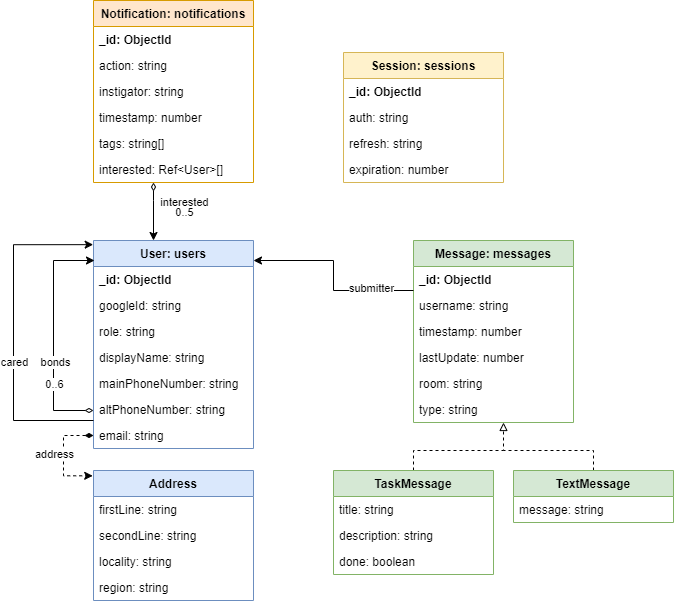
\includegraphics[width=1\textwidth]{images/Diseño/ModeloDatos.drawio.png}
    \caption{Diagrama del modelo de datos}
    \label{fig:diagrama_modelo_datos}
\end{figure}

\section{Mensaje}

Dentro de los mensaje se aúnan dos entidades de la aplicación: los \textbf{mensajes de texto} que se envían a través del Feed y las \textbf{tareas}, que también pueden ser enviadas a través del mismo. Todos estos mensajes se almacenan en la colección \emph{messages}. Aunque se puede poner en duda la elección de tratar las tareas como mensajes, esta decisión de diseño parte de un aprovechamiento de la flexibilidad de las bases de datos documentales como la que se emplea en el sistema.

Las consultas para obtener las entidades del Feed en caso de utilizar colecciones diferentes para los mensajes de texto y las tareas habría implicado la necesidad de realizar \emph{\glspl{join}}, que aunque es una operación soportada por MongoDB en sus últimas versiones, es un claro indicativo de un modelo de datos mal diseñado para bases de datos no relacionales como la nuestra. Es por eso que tanto tareas como mensajes son \textbf{incluidas en la misma colección} y tratadas ambas como mensajes al nivel de lógica de la \acrshort{api}.

\subsection{BaseMessage}

De cara a favorecer una compatibilidad lo mayor posible entre los dos tipos de entidades que se guardarán en la colección se define una primera entidad con campos comunes a ambas y que serán necesarios en las consultas a la colección. Tanto los mensajes de texto como las tareas contarán con todas las propiedades de esta clase base. Véase \fref{sch:message}.

\begin{itemize}
    \item \textbf{id}: \emph{string}. Obligatorio. Identificador único del mensaje. Generada automáticamente por MongoDB al persistir la entidad por primera vez.
    \item \textbf{submitter}: \emph{User}. Obligatorio. Referencia al usuario creador del mensaje.
    \item \textbf{username}: \emph{string}. Obligatorio. Nombre público del autor en el momento de la creación. Cacheado en este documento para evitar la necesidad de hacer \emph{\glspl{join}} con la colección de usuarios para acceder a este dato y optimizar las consultas con este tipo de base de datos.
    \item \textbf{timestamp}: \emph{number}. Obligatorio. Instante de creación del mensaje.
    \item \textbf{lastUpdate}: \emph{number}. Obligatorio. Instante de la última actualización del mensaje, si no se ha actualizado nunca desde su creación su valor será el mismo que el de \textbf{timestamp}.
    \item \textbf{room}: \emph{string}. Obligatorio. Identificador de la sala de mensajería a través de la que fue enviado el mensaje.
    \item \textbf{type}: \emph{string}. Obligatorio. Tipo de mensaje, puede ser: Text o Task.
\end{itemize}

\subsection{TaskMessage}
\label{ssec:task_message}

Representa las tareas creadas por los usuarios, tanto en la vista de Tareas como a través del Feed. Hereda de BaseMessage y su tipo es \textbf{Task}. Véase \fref{sch:task_message}. Además de las propiedades de BaseMessage cuenta con las siguientes:

\begin{itemize}
    \item \textbf{title}: \emph{string}. Obligatorio. Título de la tarea.
    \item \textbf{description}: \emph{string}. Opcional. Descripción de la tarea.
    \item \textbf{done}: \emph{boolean}. Obligatorio. Estado de la tarea, a \code{true} es hecha y \code{false} es no hecha.
\end{itemize}

\subsection{TextMessage}
\label{ssec:text_message}

Representa los mensajes de texto simples enviados a través del Feed. Hereda de BaseMessage y su tipo es \textbf{Text}. Véase \fref{sch:text_message}. Además de las propiedades de BaseMessage tiene la siguiente propiedad:

\begin{itemize}
    \item \textbf{message}: \emph{string}. Obligatorio. Cuerpo del mensaje.
\end{itemize}

\section{Notificación}

Las notificaciones reflejan una \textbf{acción de interés} para una serie de usuarios. Dicha acción se almacena en la entidad y es una de una enumeración conocida. Como algunas de estas acciones pueden servirse más de una vez, para aportar más contexto cuentan un campo para añadir etiquetas que podrán ser almacenadas y leídas según fuese necesario con cada tipo de acción.

Por otro lado, las notificaciones son \textbf{entidades compartidas} por una serie de usuarios. Los usuarios a notificar son almacenados en la entidad para su recuperación por parte de estos, una vez que un usuario marque como leída la notificación su ID será eliminada de esa lista de usuarios, de forma que la entidad pase a ir dirigida únicamente a aquellos usuarios que aún no la leyesen. Cuando una notificación ha sido leída por todos sus usuarios asociados será eliminada de la base de datos.

Las notificaciones se almacenan en la colección \emph{notifications}. El esquema definitivo se puede ver en el \fref{sch:notification}. Sus propiedades son:

\begin{itemize}
    \item \textbf{id}: \emph{string}. Obligatorio. Identificador único de la notificación. Generada automáticamente por MongoDB al persistir la entidad por primera vez.
    \item \textbf{action}: \emph{Action}. Obligatorio. Acción notificada, puede ser una de las listadas en \fref{class:api:action}.
    \item \textbf{instigator}: \emph{string}. Obligatorio. Nombre del usuario que provocó la acción a notificar.
    \item \textbf{timestamp}: \emph{number}. Obligatorio. Instante en el que ocurrió la acción.
    \item \textbf{tags}: \emph{string array}. Lista de cadenas de texto con información adicional de la notificación. Por defecto existirá como lista vacía.
    \item \textbf{interested}: \emph{User array}. Lista de referencias a los usuarios que son notificados y que aún no han leído la notificación.
\end{itemize}

\section{Sesión}
\label{ssec:sesion}

De cara a gestionar las sesiones y validar e invalidar los \glspl{token} de forma correcta, se ha creado también una colección para el almacenamiento de estas llamada \emph{sessions} (véase \fref{sch:session}). Las propiedades almacenadas son:

\begin{itemize}
    \item \textbf{id}: \emph{string}. Obligatorio. Identificador único de la sesión. Generada automáticamente por MongoDB al persistir la entidad por primera vez.
    \item \textbf{auth}: \emph{string}. Obligatorio. Es el \gls{token} activo de la sesión.
    \item \textbf{refresh}: \emph{string}. Obligatorio y único. Es el \gls{token} que permite refrescar la sesión de usuario sin necesidad de volver a autenticarse.
    \item \textbf{expiration}: \emph{number}. Obligatorio. Instante de expiración de la sesión, equivalente al tiempo de validez del \gls{token} de autenticación. Almacenado para limpiar sesiones caducadas de la base de datos.
\end{itemize}

\section{Usuario}

Los usuarios son las entidades clave de la aplicación. Su esquema en la base de datos (véase \fref{sch:user}) contiene toda la información de cada usuario, así como sus relaciones con otros usuarios. No existe una entidad diferente para Pacientes y Cuidadores. Las diferencias se gestionarán en el servicio, por lo que la entidad contiene tanto la lista de vínculos de los Pacientes como el campo para almacenar el vínculo de un Cuidador. Tiene las siguientes propiedades:

\begin{itemize}
    \item \textbf{id}: \emph{string}. Obligatorio. Identificador único del usuario. Generada automáticamente por MongoDB al persistir la entidad por primera vez.
    \item \textbf{googleId}: \emph{string}. Obligatorio y único. \Gls{token} de usuario de la cuenta de Google del usuario. Almacenada para autenticar al usuario con su cuenta de Google, no es recuperada de la base de datos al no tener ningún otro uso.
    \item \textbf{role}: \emph{Role}. Obligatorio. Rol del usuario, puede ser cualquiera de los listados en \fref{class:api:role}.
    \item \textbf{displayName}: \emph{number}. Opcional. Nombre visible del usuario.
    \item \textbf{mainPhoneNumber}: \emph{string}. Opcional. Número de teléfono principal del usuario.
    \item \textbf{altPhoneNumber}: \emph{string}. Opcional. Número de teléfono alternativo del usuario.
    \item \textbf{address}: \emph{Address}. Opcional. Dirección postal del usuario (véase \fref{ss:address}).
    \item \textbf{email}: \emph{string}. Opcional. Dirección electrónica del usuario.
    \item \textbf{bonds}: \emph{User array}. Opcional. Lista de referencias a los usuarios vinculados con un Paciente.
    \item \textbf{cared}: \emph{User}. Opcional. Referencia al Paciente vinculado de un Cuidador.
\end{itemize}

\subsection{Address}
\label{ss:address}

Representación de las direcciones postales como objetos del sistema, compuesta por las siguientes propiedades:

\begin{itemize}
    \item \textbf{firstLine}: \emph{string}. Opcional. Primera línea de la dirección para la información principal.
    \item \textbf{secondLine}: \emph{string}. Opcional. Segunda línea de la dirección para la información principal.
    \item \textbf{locality}: \emph{string}. Opcional. Localidad.
    \item \textbf{region}: \emph{string}. Opcional. Región.
\end{itemize}                        
\chapter{Interfaces de comunicación}
\label{ch:interfaces_comunicacion}

\section{API REST}

A continuación se describen los \glspl{endpoint} de la API REST del sistema y toda la información de su funcionamiento. El único \gls{endpoint} público de la interfaz es el de inicio de sesión (\ref{api:inicio_sesion}), el token de autenticación provisto en las llamadas exitosas a dicho \gls{endpoint} será el que se deba proveer en el encabezado de autenticación siguiendo el \textbf{RFC 6750}\cite{rfc6750} para poder acceder a las funcionalidades del resto de funciones de la interfaz.

Cualquier petición a los \glspl{endpoint} privados puede provocar los siguientes errores de autenticación aparte de los inherentes de cada función:

\begin{itemize}
    \item 400 BAD REQUEST si falta el Authorization header o está mal formateado.
    \item 401 UNAUTHORIZED si el \gls{token} es inválido o está expirado.
\end{itemize}

\vspace{-10pt}
\subsection{Autenticación}

% GET /auth/session/:token
\begin{longtable}{|p{0.25\textwidth} p{0.75\textwidth}|}
    \hline
    \multicolumn{2}{|l|}{\textbf{Inicio de sesión}} \\ \hline 
    Descripción         & Inicia la sesión del usuario en el sistema con su token de autenticación en Google y responde con los tokens de la sesión y la información del usuario. Si el usuario no existe, lo crea. \\ \hline \hline
    \multicolumn{2}{|l|}{\emph{Petición}}  \\ \hline 
    URL      & /auth/session/:token \\ \hline
    Método   & GET                  \\ \hline
    Parámetros URL  & 
    \textbf{token}: \emph{string}. Token de sesión obtenido tras la autenticación exitosa en el servicio de \emph{Google Auth} \\ \hline \hline
    \multicolumn{2}{|l|}{\emph{Respuesta}} \\ \hline 
    Código          & 200 OK          \\ \hline
    Content-type    & application-json  \\ \hline
    Cuerpo  & 
    \textbf{session}: \emph{object}. \acrshort{dto} de la sesión iniciada (\ref{dto:session}) \\
    & \textbf{user}: \emph{object}. Contiene toda la información del usuario en un \nameref{dto:user} (\ref{dto:user})
    \\ \hline \hline
    Errores & 400 BAD REQUEST si el token proporcionado no pasa la validación de Google. 
    \\ \hline
    \caption{Documentación del endpoint de inicio de sesión}
    \label{api:inicio_sesion}
\end{longtable}

% DELETE /auth/session/:token
\begin{longtable}{|p{0.25\textwidth} p{0.75\textwidth}|}
    \hline
    \multicolumn{2}{|l|}{\textbf{Cierre de sesión}} \\ \hline 
    Descripción         & Cierre la sesión del usuario en el sistema con su token de autenticación. \\ \hline \hline
    \multicolumn{2}{|l|}{\emph{Petición}}  \\ \hline 
    URL      & /auth/session/:token \\ \hline
    Método   & DELETE                  \\ \hline
    Encabezados  & 
    \textbf{Authorization}: Token de sesión según RFC6750. \\ \hline
    Parámetros URL  & 
    \textbf{token}: \emph{string}. Token de autenticación de la sesión a cerrar \\ \hline \hline
    \multicolumn{2}{|l|}{\emph{Respuesta}} \\ \hline 
    Código          & 204 NO CONTENT          \\ \hline \hline
    Errores & 403 FORBIDDEN si el token proporcionado no pertenece al usuario realizando la petición. 
    \\ \hline
    \caption{Documentación del endpoint de cierre de sesión}
    \label{api:cierre_sesion}
\end{longtable}

% GET /auth/refresh/:token
\begin{longtable}{|p{0.25\textwidth} p{0.75\textwidth}|}
    \hline
    \multicolumn{2}{|l|}{\textbf{Refresco de sesión}} \\ \hline 
    Descripción         & Renueva la sesión de usuario y devuelve los nuevos tokens de sesión \\ \hline \hline
    \multicolumn{2}{|l|}{\emph{Petición}}  \\ \hline 
    URL      & /auth/refresh/:token \\ \hline
    Método   & GET                  \\ \hline
    Encabezados  & 
    \textbf{Authorization}: Token de sesión según RFC6750 \\ \hline
    Parámetros URL  & 
    \textbf{token}: \emph{string}. Token de refresco de la sesión a renovar \\ \hline \hline
    \multicolumn{2}{|l|}{\emph{Respuesta}} \\ \hline 
    Código          & 200 OK          \\ \hline
    Content-type    & application-json  \\ \hline
    Cuerpo  & 
    \textbf{session}: \emph{object}. \acrshort{dto} de la sesión refrescada (\ref{dto:session}) \\ \hline \hline
    Errores & 400 BAD REQUEST si no existe la sesión abierta a la que los tokens están asignados \\     
        & 401 UNAUTHORIZED si los tokens proporcionados en la petición no son válidos \\
        & 401 UNAUTHORIZED si el token de refresco está expirado \\
        & 401 UNAUTHORIZED si el token de refresco es inválido.
    \\ \hline
    \caption{Documentación del endpoint de refresco de sesión}
    \label{api:refresco_sesion}
\end{longtable}
\subsection{Feed}

%feed:join
\begin{longtable}{|p{0.25\textwidth} p{0.75\textwidth}|}
    \hline
    \multicolumn{2}{|l|}{\textbf{FEED\textunderscore JOIN}} \\ \hline 
    Descripción         & Suscribe a un cliente a una sala de mensajería. \\ \hline
    Clave               & feed:join \\ \hline
    Tipo                & Retransmisión \\ \hline \hline
    Mensaje de entrada  &      
   \emph{object}. \acrshort{dto} con la información del usuario, del tipo \nameref{dto:usermin} (\fref{dto:usermin}). \\ \hline \hline
    Emisión   & FEED\textunderscore JOIN a los usuarios suscritos a la sala. \\ \hline \hline
    Errores     & Si el cliente no está conectado a una sala global .\\ \hline
    \caption{Documentación del evento Join de la sala Feed}
    \label{ws:feed_join}
\end{longtable}

%feed:leave
\begin{longtable}{|p{0.25\textwidth} p{0.75\textwidth}|}
    \hline
    \multicolumn{2}{|l|}{\textbf{FEED\textunderscore LEAVE}} \\ \hline 
    Descripción         & Da de baja a un cliente de su sala de mensajería. \\ \hline
    Clave               & feed:leave \\ \hline
    Tipo                & Retransmisión \\ \hline \hline
    Mensaje de entrada  &      
   \emph{object}. \acrshort{dto} con la información del usuario, del tipo \nameref{dto:usermin} (\fref{dto:usermin}). \\ \hline \hline
    Emisión
    & FEED\textunderscore LEAVE a los usuarios suscritos a la sala \\  \hline \hline
    Errores     & Si el cliente no está conectado a una sala de mensajería. \\ \hline
    \caption{Documentación del evento Leave de la sala Feed}
    \label{ws:feed_leave}
\end{longtable}

%feed:send
\begin{table}[H]
\begin{longtable}{|p{0.25\textwidth} p{0.75\textwidth}|}
    \hline
    \multicolumn{2}{|l|}{\textbf{FEED\textunderscore SEND}} \\ \hline 
    Descripción         & Envía un mensaje a través de la sala. \\ \hline
    Clave               & feed:send \\ \hline
    Tipo                & Cliente \\ \hline \hline
    Mensaje de entrada    &
   \emph{object}. \acrshort{dto} del mensaje, del tipo \nameref{dto:message} (\fref{dto:message}). \\ \hline \hline
    Emisión
    & FEED\textunderscore NEW a los usuarios suscritos a la sala \\ \hline \hline
    Errores     & Si el cliente no está conectado a una sala de mensajería \\ \hline
    \caption{Documentación del evento Send de la sala Feed}
    \label{ws:feed_send}
\end{longtable}
\end{table}

\newpage

%feed:new
\begin{longtable}{|p{0.25\textwidth} p{0.75\textwidth}|}
    \hline
    \multicolumn{2}{|l|}{\textbf{FEED\textunderscore NEW}} \\ \hline 
    Descripción         & Nuevo mensaje enviado a través de la sala. \\ \hline
    Clave               & feed:new \\ \hline
    Tipo                & Servidor \\ \hline \hline
    Emisión    &
   \emph{object}. \acrshort{dto} del mensaje, del tipo \nameref{dto:message} (\fref{dto:message}). \\ \hline
    \caption{Documentación del evento New de la sala Feed}
    \label{ws:feed_new}
\end{longtable}

%feed:delete
\begin{longtable}{|p{0.25\textwidth} p{0.75\textwidth}|}
    \hline
    \multicolumn{2}{|l|}{\textbf{FEED\textunderscore DELETE}} \\ \hline 
    Descripción         & Elimina un mensaje eviado a través de la sala. \\ \hline
    Clave               & feed:delete \\ \hline
    Tipo                & Servidor \\ \hline \hline
    Emisión    &
   \emph{object}. \acrshort{dto} del mensaje, del tipo \nameref{dto:message} (\fref{dto:message}). \\ \hline
    \caption{Documentación del evento Delete de la sala Feed}
    \label{ws:feed_delete}
\end{longtable}

\subsection{Tareas}

\vspace{-10pt}
% POST /tasks 
\begin{longtable}{|p{0.25\textwidth} p{0.75\textwidth}|}
    \hline
    \multicolumn{2}{|l|}{\textbf{Crear tarea}} \\ \hline 
    Descripción         & Persiste y completa la tarea enviada. \\ \hline \hline
    \multicolumn{2}{|l|}{\emph{Petición}}  \\ \hline 
    URL      & /tasks \\ \hline
    Método   & POST                  \\ \hline
    Encabezados  & 
    \textbf{Authorization}: Token de sesión según RFC6750. \\ \hline
    Cuerpo  & \emph{object}. Tarea a persistir con las propiedades de \nameref{dto:taskmin} (\ref{dto:taskmin}). \\ \hline \hline
    \multicolumn{2}{|l|}{\emph{Respuesta}} \\ \hline 
    Código          & 201 CREATED          \\ \hline
    Content-type    & application-json  \\ \hline
    Cuerpo  & 
    \emph{object}. \acrshort{dto} de la tarea creada con las propiedades de \nameref{dto:taskmessage} (\ref{dto:taskmessage}). \\ \hline \hline
    Errores & 400 BAD REQUEST si el usuario es un Cuidador no vinculado.
    \\ \hline
    \caption{Documentación del endpoint de crear una tarea}
    \label{api:crear_tarea}
\end{longtable}

% GET /tasks 
\begin{table}[H]
\begin{longtable}{|p{0.25\textwidth} p{0.75\textwidth}|}
    \hline
    \multicolumn{2}{|l|}{\textbf{Recuperar tareas relevantes}} \\ \hline 
    Descripción         & Devuelve la lista de tareas relevantes del usuario. Una tarea relevante es aquella incompleta o que ha sido actualizada alguna vez en el margen de días máximo especificado en la petición. \\ \hline \hline
    \multicolumn{2}{|l|}{\emph{Petición}}  \\ \hline 
    URL      & /tasks \\ \hline
    Método   & GET                  \\ \hline
    Encabezados  & 
    \textbf{Authorization}: Token de sesión según RFC6750. \\ \hline
    Parámetros consulta  & 
    \textbf{maxDays}: \emph{number}. \emph{Opcional}. Número de días máximo desde la última actualización de las tareas completadas para considerarlas relevantes. Por defecto, 3 días. \\ \hline \hline
    \multicolumn{2}{|l|}{\emph{Respuesta}} \\ \hline 
    Código          & 200 OK          \\ \hline
    Content-type    & application-json  \\ \hline
    Cuerpo  & 
    \textbf{tasks}: \emph{object array}. Lista de tareas recuperadas de tipo \nameref{dto:taskmessage} (\ref{dto:taskmessage}). \\ \hline \hline
    Errores & 400 BAD REQUEST si el usuario es un Cuidador no vinculado
    \\ \hline
    \caption{Documentación del endpoint de recuperar tareas relevantes}
    \label{api:recuperar_tarea}
\end{longtable}
\end{table}

% DELETE /tasks/:id
\begin{longtable}{|p{0.25\textwidth} p{0.75\textwidth}|}
    \hline
    \multicolumn{2}{|l|}{\textbf{Eliminar tarea}} \\ \hline 
    Descripción         & Elimina la tarea especificada. \\ \hline \hline
    \multicolumn{2}{|l|}{\emph{Petición}}  \\ \hline 
    URL      & /tasks/:id \\ \hline
    Método   & DELETE                  \\ \hline
    Encabezados  & 
    \textbf{Authorization}: Token de sesión según RFC6750. \\ \hline
    Parámetros URL  & 
    \textbf{id}: \emph{string}. Identificador único de la tarea a eliminar. \\ \hline \hline
    \multicolumn{2}{|l|}{\emph{Respuesta}} \\ \hline 
    Código          & 204 NO CONTENT          \\ \hline \hline
    Errores & 403 FORBIDDEN si el usuario no tiene permisos para eliminar la tarea
    \\ \hline
    \caption{Documentación del endpoint de eliminar una tarea}
    \label{api:eliminar_tarea}
\end{longtable}

% POST /tasks:/:id/done
\begin{table}[H]
\begin{longtable}{|p{0.25\textwidth} p{0.75\textwidth}|}
    \hline
    \multicolumn{2}{|l|}{\textbf{Marcar tarea como hecha}} \\ \hline 
    Descripción         & Marca la tarea especificada como hecha. \\ \hline \hline
    \multicolumn{2}{|l|}{\emph{Petición}}  \\ \hline 
    URL      & /tasks/:id/done \\ \hline
    Método   & POST                  \\ \hline
    Encabezados  & 
    \textbf{Authorization}: Token de sesión según RFC6750. \\ \hline
    Parámetros URL  & 
    \textbf{id}: \emph{string}. Identificador único de la tarea a actualizar. \\ \hline \hline
    \multicolumn{2}{|l|}{\emph{Respuesta}} \\ \hline 
    Código          & 204 NO CONTENT          \\ \hline  \hline
    Errores & 403 FORBIDDEN si el usuario no tiene permisos para actualizar la tarea
    \\ \hline
    \caption{Documentación del endpoint de marcar una tarea como hecha}
    \label{api:marcar_tarea_hecha}
\end{longtable}
\end{table}

% DELETE /tasks:/:id/done
\begin{longtable}{|p{0.25\textwidth} p{0.75\textwidth}|}
    \hline
    \multicolumn{2}{|l|}{\textbf{Marcar tarea como no hecha}} \\ \hline 
    Descripción         & Marca la tarea especificada como no hecha. \\ \hline \hline
    \multicolumn{2}{|l|}{\emph{Petición}}  \\ \hline 
    URL      & /tasks/:id/done \\ \hline
    Método   & DELETE                  \\ \hline
    Encabezados  & 
    \textbf{Authorization}: Token de sesión según RFC6750. \\ \hline
    Parámetros URL  & 
    \textbf{id}: \emph{string}. Identificador único de la tarea a actualizar. \\ \hline \hline
    \multicolumn{2}{|l|}{\emph{Respuesta}} \\ \hline 
    Código          & 204 NO CONTENT          \\ \hline \hline
    Errores & 403 FORBIDDEN si el usuario no tiene permisos para actualizar la tarea
    \\ \hline
    \caption{Documentación del endpoint de marcar una tarea como no hecha}
    \label{api:marcar_tarea_no_hecha}
\end{longtable}

\newpage
\subsection{Usuarios}

% PATCH /user/:id
\begin{longtable}{|p{0.25\textwidth} p{0.75\textwidth}|}
    \hline
    \multicolumn{2}{|l|}{\textbf{Actualizar usuario}} \\ \hline 
    Descripción         & Actualiza la información de un usuario. \\ \hline \hline
    \multicolumn{2}{|l|}{\emph{Petición}}  \\ \hline 
    URL      & /user/:id \\ \hline
    Método   & PATCH                  \\ \hline
    Encabezados  & 
    \textbf{Authorization}: Token de sesión según RFC6750. \\ \hline
    Parámetros URL  & 
    \textbf{id}: \emph{string}. Identificador único del usuario. \\ \hline
    Cuerpo &
    \emph{object}. Propiedades a actualizar del usuario en un \acrshort{dto} de tipo \nameref{dto:userpublic} (\ref{dto:userpublic}). \\ \hline \hline
    \multicolumn{2}{|l|}{\emph{Respuesta}} \\ \hline 
    Código          & 201 CREATED         \\ \hline
    Content-type    & application-json  \\ \hline
    Cuerpo  & 
    \emph{object}. Información del usuario de tipo \nameref{dto:user} (\ref{dto:user}) \\ \hline \hline
    Errores & 403 FORBIDDEN si el solicitante no es el usuario que intenta actualizar.
    \\ \hline
    \caption{Documentación del endpoint de actualización de información de usuarios}
    \label{api:actualizar_usuario}
\end{longtable}

% GET /user/bonds/token 
\begin{longtable}{|p{0.25\textwidth} p{0.75\textwidth}|}
    \hline
    \multicolumn{2}{|l|}{\textbf{Generar token de vinculación}} \\ \hline 
    Descripción         & Devuelve un token de vinculación válido del usuario. \\ \hline \hline
    \multicolumn{2}{|l|}{\emph{Petición}}  \\ \hline 
    URL      & /user/bonds/token \\ \hline
    Método   & GET                  \\ \hline
    Encabezados  & 
    \textbf{Authorization}: Token de sesión según RFC6750. \\ \hline  \hline
    \multicolumn{2}{|l|}{\emph{Respuesta}} \\ \hline 
    Código          & 200 OK         \\ \hline
    Content-type    & application-json  \\ \hline
    Cuerpo  & 
    \textbf{code}: \emph{string}. Token de vinculación. \\ \hline
    \caption{Documentación del endpoint de generación de tokens de vinculación}
    \label{api:generar_token_vinculacion}
\end{longtable}

\newpage
% POST /user/bonds/token 
\begin{longtable}{|p{0.25\textwidth} p{0.75\textwidth}|}
    \hline
    \multicolumn{2}{|l|}{\textbf{Establecer vínculos}} \\ \hline 
    Descripción         & Valida el token de vinculación enviado y crea el vínculo entre los dos usuarios si es correcto. \\ \hline \hline
    \multicolumn{2}{|l|}{\emph{Petición}}  \\ \hline 
    URL      & /user/bonds/token \\ \hline
    Método   & POST                  \\ \hline
    Encabezados  & 
    \textbf{Authorization}: Token de sesión según RFC6750. \\ \hline
    Parámetros URL  & 
    \textbf{code}: \emph{string}. Token de vinculación. \\ \hline \hline
    \multicolumn{2}{|l|}{\emph{Respuesta}} \\ \hline 
    Código          & 200 OK         \\ \hline
    Content-type    & application-json  \\ \hline
    Cuerpo  & 
    \textbf{message}: \emph{string}. Mensaje de confirmación de la acción. \\ \hline \hline
    Errores & 400 BAD REQUEST si el token ha expirado. \\
            & 400 BAD REQUEST si el Paciente ya tiene el máximo de vínculos \\
            & 400 BAD REQUEST si el Cuidador ya está vinculado \\
            & 403 FORBIDDEN si el usuario es un Paciente
    \\ \hline
    \caption{Documentación del endpoint de establecimiento de vínculos}
    \label{api:establecer_vinculo}
\end{longtable}

% DELETE /user/bonds/:id 
\begin{longtable}{|p{0.25\textwidth} p{0.75\textwidth}|}
    \hline
    \multicolumn{2}{|l|}{\textbf{Eliminar vínculos}} \\ \hline 
    Descripción         & Elimina el vínculo con el usuario especificado. \\ \hline \hline
    \multicolumn{2}{|l|}{\emph{Petición}}  \\ \hline 
    URL      & /user/bonds/:id \\ \hline
    Método   & DELETE                  \\ \hline
    Encabezados  & 
    \textbf{Authorization}: Token de sesión según RFC6750. \\ \hline
    Cuerpo  & 
    \textbf{id}: \emph{string}. ID del usuario a desvincular. \\ \hline \hline
    \multicolumn{2}{|l|}{\emph{Respuesta}} \\ \hline 
    Código          & 204 NO CONTENT         \\ \hline \hline
    \caption{Documentación del endpoint de eliminación de vínculos}
    \label{api:eliminar_vinculo}
\end{longtable}

\newpage
% GET /user/:id/cared 
\begin{longtable}{|p{0.25\textwidth} p{0.75\textwidth}|}
    \hline
    \multicolumn{2}{|l|}{\textbf{Recuperar Paciente vinculado}} \\ \hline 
    Descripción         & Recupera la información del Paciente vinculado al usuario. \\ \hline \hline
    \multicolumn{2}{|l|}{\emph{Petición}}  \\ \hline 
    URL      & /user/:id/cared \\ \hline
    Método   & GET                  \\ \hline
    Encabezados  & 
    \textbf{Authorization}: Token de sesión según RFC6750. \\ \hline
    Parámetros URL  & 
    \textbf{id}: \emph{string}. Identificador único del usuario. \\ \hline  \hline
    \multicolumn{2}{|l|}{\emph{Respuesta}} \\ \hline 
    Código          & 200 OK         \\ \hline
    Content-type    & application-json  \\ \hline
    Cuerpo  & 
    \textbf{cared}: \emph{object}. Información del Paciente vinculado en un \acrshort{dto} de tipo \nameref{dto:user} (\ref{dto:user}). \\ \hline \hline
    Errores & 400 BAD REQUEST si el usuario no es un Cuidador. \\
            & 403 FORBIDDEN si el solicitante no es el usuario del que pretende obtener el Paciente vinculado. \\ \hline
    \caption{Documentación del endpoint de actualización de información de usuarios}
    \label{api:recuperar_paciente}
\end{longtable}

% GET /user/bonds 
\begin{longtable}{|p{0.25\textwidth} p{0.75\textwidth}|}
    \hline
    \multicolumn{2}{|l|}{\textbf{Recuperar información de asociados}} \\ \hline 
    Descripción         & Devuelve la información de contacto de los usuarios asociados con el solicitante. \\ \hline \hline
    \multicolumn{2}{|l|}{\emph{Petición}}  \\ \hline 
    URL      & /user/bonds \\ \hline
    Método   & GET                  \\ \hline
    Encabezados  & 
    \textbf{Authorization}: Token de sesión según RFC6750. \\ \hline \hline
    \multicolumn{2}{|l|}{\emph{Respuesta}} \\ \hline 
    Código          & 200 OK         \\ \hline
    Content-type    & application-json  \\ \hline
    Cuerpo  & 
    \textbf{bonds}: \emph{object array}. Lista de información de contacto de los asociados del usuario. Enviados en \acrshort{dto}s de tipo \nameref{dto:userpublic} (\ref{dto:userpublic}) \\ \hline \hline
    Errores & 400 BAD REQUEST si el usuario no es Paciente ni Cuidador \\
            & 403 FORBIDDEN si el solicitante no es el usuario que intenta actualizar.
    \\ \hline
    \caption{Documentación del endpoint de recuperación de información de asociados}
    \label{api:recuperar_asociados}
\end{longtable}


\section{API del WebSocket}

El otro tipo de comunicación ofrecido por la API es la que se produce a través del WebSocket. Esta comunicación se produce de forma \textbf{no bidireccional} por medio de envío de mensajes de texto con una clave que indica el evento que invoca. Las peticiones de un cliente (mensajes de cliente o entrada) serán enviados al servidor y no se quedarán esperando una respuesta, y si esta se produce será por medio de otro evento enviado por el servidor (mensaje de servidor o salida). Si una solicitud de un cliente tiene algún error, el mensaje será ignorado. Algunos mensaje de cliente pueden ser remitidos por el servidor con la misma clave de evento, estos mensajes constituyen un nuevo tipo de comunicación llamado \textbf{retransmisión}.

Todo cliente que se suscriba al socket debe unirse a una habitación global compartida entre todos los usuarios asociados. Es a través de esta sala que se gestiona la unión al resto de salas. La desconexión de esta sala supondría la desconexión del resto de salas. La sala global cuenta con dos eventos ilustrados en \fref{ws:global_subscribe} y \fref{ws:global_subscription}.

% global:subscribe
\begin{longtable}{|p{0.25\textwidth} p{0.75\textwidth}|}
    \hline
    \multicolumn{2}{|l|}{\textbf{GLOBAL\textunderscore SUBSCRIBE}} \\ \hline 
    Descripción         & Suscribe a un cliente a una sala global. \\ \hline
    Clave               & global:subscribe \\ \hline
    Tipo                & Cliente \\ \hline \hline
    Mensaje de entrada  &      
   \emph{string}. ID del usuario solicitando unirse a la sala. \\ \hline \hline
    Emisión   & GLOBAL\textunderscore SUBSCRIPTION (\ref{ws:global_subscription}) a los usuarios suscritos a la sala \\ \hline \hline
    Errores     & Si el cliente no es Paciente ni Cuidador \\
                & Si el cliente es un Cuidador no vinculado \\ \hline
    \caption{Documentación del evento Subscribe de la sala Global}
    \label{ws:global_subscribe}
\end{longtable}

% global:subscription
\begin{longtable}{|p{0.25\textwidth} p{0.75\textwidth}|}
    \hline
    \multicolumn{2}{|l|}{\textbf{GLOBAL\textunderscore SUBSCRIPTION}} \\ \hline 
    Descripción         & Notificación a los suscriptores de una sala acerca de la suscripción de un nuevo cliente. \\ \hline
    Clave               & global:subscription \\ \hline
    Tipo                & Servidor \\ \hline \hline
    Emisión      
    & \textbf{user}: \emph{string}. ID del nuevo suscriptor. \\
    & \textbf{roomId}: \emph{string}. ID de la sala. \\ \hline
    \caption{Documentación del evento Subscription de la sala Global}
    \label{ws:global_subscription}
\end{longtable}

\subsection{Feed}

%feed:join
\begin{longtable}{|p{0.25\textwidth} p{0.75\textwidth}|}
    \hline
    \multicolumn{2}{|l|}{\textbf{FEED\textunderscore JOIN}} \\ \hline 
    Descripción         & Suscribe a un cliente a una sala de mensajería. \\ \hline
    Clave               & feed:join \\ \hline
    Tipo                & Retransmisión \\ \hline \hline
    Mensaje de entrada  &      
   \emph{object}. \acrshort{dto} con la información del usuario, del tipo \nameref{dto:usermin} (\fref{dto:usermin}). \\ \hline \hline
    Emisión   & FEED\textunderscore JOIN a los usuarios suscritos a la sala. \\ \hline \hline
    Errores     & Si el cliente no está conectado a una sala global .\\ \hline
    \caption{Documentación del evento Join de la sala Feed}
    \label{ws:feed_join}
\end{longtable}

%feed:leave
\begin{longtable}{|p{0.25\textwidth} p{0.75\textwidth}|}
    \hline
    \multicolumn{2}{|l|}{\textbf{FEED\textunderscore LEAVE}} \\ \hline 
    Descripción         & Da de baja a un cliente de su sala de mensajería. \\ \hline
    Clave               & feed:leave \\ \hline
    Tipo                & Retransmisión \\ \hline \hline
    Mensaje de entrada  &      
   \emph{object}. \acrshort{dto} con la información del usuario, del tipo \nameref{dto:usermin} (\fref{dto:usermin}). \\ \hline \hline
    Emisión
    & FEED\textunderscore LEAVE a los usuarios suscritos a la sala \\  \hline \hline
    Errores     & Si el cliente no está conectado a una sala de mensajería. \\ \hline
    \caption{Documentación del evento Leave de la sala Feed}
    \label{ws:feed_leave}
\end{longtable}

%feed:send
\begin{table}[H]
\begin{longtable}{|p{0.25\textwidth} p{0.75\textwidth}|}
    \hline
    \multicolumn{2}{|l|}{\textbf{FEED\textunderscore SEND}} \\ \hline 
    Descripción         & Envía un mensaje a través de la sala. \\ \hline
    Clave               & feed:send \\ \hline
    Tipo                & Cliente \\ \hline \hline
    Mensaje de entrada    &
   \emph{object}. \acrshort{dto} del mensaje, del tipo \nameref{dto:message} (\fref{dto:message}). \\ \hline \hline
    Emisión
    & FEED\textunderscore NEW a los usuarios suscritos a la sala \\ \hline \hline
    Errores     & Si el cliente no está conectado a una sala de mensajería \\ \hline
    \caption{Documentación del evento Send de la sala Feed}
    \label{ws:feed_send}
\end{longtable}
\end{table}

\newpage

%feed:new
\begin{longtable}{|p{0.25\textwidth} p{0.75\textwidth}|}
    \hline
    \multicolumn{2}{|l|}{\textbf{FEED\textunderscore NEW}} \\ \hline 
    Descripción         & Nuevo mensaje enviado a través de la sala. \\ \hline
    Clave               & feed:new \\ \hline
    Tipo                & Servidor \\ \hline \hline
    Emisión    &
   \emph{object}. \acrshort{dto} del mensaje, del tipo \nameref{dto:message} (\fref{dto:message}). \\ \hline
    \caption{Documentación del evento New de la sala Feed}
    \label{ws:feed_new}
\end{longtable}

%feed:delete
\begin{longtable}{|p{0.25\textwidth} p{0.75\textwidth}|}
    \hline
    \multicolumn{2}{|l|}{\textbf{FEED\textunderscore DELETE}} \\ \hline 
    Descripción         & Elimina un mensaje eviado a través de la sala. \\ \hline
    Clave               & feed:delete \\ \hline
    Tipo                & Servidor \\ \hline \hline
    Emisión    &
   \emph{object}. \acrshort{dto} del mensaje, del tipo \nameref{dto:message} (\fref{dto:message}). \\ \hline
    \caption{Documentación del evento Delete de la sala Feed}
    \label{ws:feed_delete}
\end{longtable}

\subsection{Localización}

% location:share
\begin{longtable}{|p{0.25\textwidth} p{0.75\textwidth}|}
    \hline
    \multicolumn{2}{|l|}{\textbf{LOCATION\textunderscore SHARE}} \\ \hline 
    Descripción         & Suscribe a un cliente a una sala de geolocalización. \\ \hline
    Clave               & location:share \\ \hline
    Tipo                & Cliente \\ \hline \hline
    Mensaje de entrada  &      
   \emph{object}. \acrshort{dto} con la información del usuario, del tipo \nameref{dto:usermin} (\fref{dto:usermin}). \\ \hline \hline
    Emisión   & NOTIFY\textunderscore LOCATION\textunderscore SHARING\textunderscore START (\ref{ws:notify_location_sharing_start}) a los usuarios suscritos a la sala \\ \hline \hline
    Errores     & Si el cliente no está conectado a una sala global \\ \hline
    \caption{Documentación del evento Share de la sala Location}
    \label{ws:location_subscribe}
\end{longtable}

\newpage

% location:stop
\begin{longtable}{|p{0.25\textwidth} p{0.75\textwidth}|}
    \hline
    \multicolumn{2}{|l|}{\textbf{LOCATION\textunderscore STOP}} \\ \hline 
    Descripción         & Da de baja a un cliente de su sala de localización. \\ \hline
    Clave               & location:stop \\ \hline
    Tipo                & Retransmisión \\ \hline \hline
    Mensaje de entrada  &      
   \emph{object}. \acrshort{dto} con la información del usuario, del tipo \nameref{dto:usermin} (\fref{dto:usermin}). \\ \hline \hline
    Emisión
    & LOCATION\textunderscore STOP a los usuarios suscritos a la sala \\
    & NOTIFY\textunderscore LOCATION\textunderscore SHARING\textunderscore STOP (\ref{ws:notify_location_sharing_stop}) a los usuarios asociados conectados \\ \hline \hline
    Errores     & Si el cliente no está conectado a una sala de localización \\ \hline
    \caption{Documentación del evento Stop de la sala Location}
    \label{ws:location_stop}
\end{longtable}

\vspace{-20pt}
% location:update
\begin{longtable}{|p{0.25\textwidth} p{0.75\textwidth}|}
    \hline
    \multicolumn{2}{|l|}{\textbf{LOCATION\textunderscore UPDATE}} \\ \hline 
    Descripción         & Comparte la ubicación de un usuario. \\ \hline
    Clave               & location:update \\ \hline
    Tipo                & Retransmisión \\ \hline \hline
    Mensaje de entrada    
   & \textbf{id}: \emph{string}. ID del usuario. \\
   & \textbf{displayName}: \emph{string}. Nombre público del usuario. \\
   & \textbf{position}: \emph{object}. Compuesto por \textbf{latitute}:\emph{number} y \textbf{longitude}:\emph{number}. La posición a compartir. \\ \hline \hline
    Emisión
    & LOCATION\textunderscore UPDATE al resto de usuarios suscritos a la sala \\ \hline \hline
    Errores     & Si el cliente no está conectado a una sala de localización \\ \hline
    \caption{Documentación del evento Update de la sala Location}
    \label{ws:location_update}
\end{longtable}

\vspace{-30pt}
\subsection{Notificación}
\vspace{-10pt}

Los eventos de notificaciones no cuentan con su propia sala sino que son emitidas a través de la sala global y son todos de tipo servidor pues son mensajes generados por el usuario a raíz de acciones transversales que son comunicadas a los usuarios relevantes.

%notify:bond_created
\begin{longtable}{|p{0.25\textwidth} p{0.75\textwidth}|}
    \hline
    \multicolumn{2}{|l|}{\textbf{NOTIFY\textunderscore BOND\textunderscore CREATED}} \\ \hline 
    Descripción         & Notifica la creación de un vínculo. \\ \hline
    Clave               & notify:bond\textunderscore created \\ \hline
    Tipo                & Servidor \\ \hline \hline
    Emisión    &
   \emph{object}. \acrshort{dto} de la notificación, del tipo \nameref{dto:notification} (\fref{dto:notification}). \\ \hline
    \caption{Documentación del evento Notify Bond Created de la sala Global}
    \label{ws:notify_bond_created}
\end{longtable}

%notify:bond_deleted
\begin{longtable}{|p{0.25\textwidth} p{0.75\textwidth}|}
    \hline
    \multicolumn{2}{|l|}{\textbf{NOTIFY\textunderscore BOND\textunderscore DELETED}} \\ \hline 
    Descripción         & Notifica la eliminación de un vínculo. \\ \hline
    Clave               & notify:bond\textunderscore deleted \\ \hline
    Tipo                & Servidor \\ \hline \hline
    Emisión    &
   \emph{object}. \acrshort{dto} de la notificación, del tipo \nameref{dto:notification} (\fref{dto:notification}). \\ \hline
    \caption{Documentación del evento Notify Bond Deleted de la sala Global}
    \label{ws:notify_bond_deleted}
\end{longtable}

%notify:task_deleted
\begin{longtable}{|p{0.25\textwidth} p{0.75\textwidth}|}
    \hline
    \multicolumn{2}{|l|}{\textbf{NOTIFY\textunderscore TASK\textunderscore DELETED}} \\ \hline 
    Descripción         & Notifica la eliminación de una tarea. \\ \hline
    Clave               & notify:task\textunderscore deleted \\ \hline
    Tipo                & Servidor \\ \hline \hline
    Emisión    &
   \emph{object}. \acrshort{dto} de la notificación, del tipo \nameref{dto:notification} (\fref{dto:notification}). \\ \hline
    \caption{Documentación del evento Notify Task Deleted de la sala Global}
    \label{ws:notify_task_deleted}
\end{longtable}

%notify:task_done
\begin{longtable}{|p{0.25\textwidth} p{0.75\textwidth}|}
    \hline
    \multicolumn{2}{|l|}{\textbf{NOTIFY\textunderscore TASK\textunderscore DONE}} \\ \hline 
    Descripción         & Notifica el cambio de una tarea a hecha. \\ \hline
    Clave               & notify:task\textunderscore done \\ \hline
    Tipo                & Servidor \\ \hline \hline
    Emisión    &
   \emph{object}. \acrshort{dto} de la notificación, del tipo \nameref{dto:notification} (\fref{dto:notification}). \\ \hline
    \caption{Documentación del evento Notify Task Done de la sala Global}
    \label{ws:notify_task_done}
\end{longtable}

%notify:task_undone
\begin{longtable}{|p{0.25\textwidth} p{0.75\textwidth}|}
    \hline
    \multicolumn{2}{|l|}{\textbf{NOTIFY\textunderscore TASK\textunderscore UNDONE}} \\ \hline 
    Descripción         & Notifica el cambio de una tarea a no hecha. \\ \hline
    Clave               & notify:task\textunderscore undone \\ \hline
    Tipo                & Servidor \\ \hline \hline
    Emisión    &
   \emph{object}. \acrshort{dto} de la notificación, del tipo \nameref{dto:notification} (\fref{dto:notification}). \\ \hline
    \caption{Documentación del evento Notify Task Undone de la sala Global}
    \label{ws:notify_task_undone}
\end{longtable}

%notify:location_sharing_start
\begin{longtable}{|p{0.25\textwidth} p{0.75\textwidth}|}
    \hline
    \multicolumn{2}{|l|}{\textbf{NOTIFY\textunderscore LOCATION\textunderscore SHARING\textunderscore START}} \\ \hline 
    Descripción         & Notifica que un usuario asociado ha comenzado a compartir su ubicación. \\ \hline
    Clave               & notify:location\textunderscore sharing\textunderscore start \\ \hline
    Tipo                & Servidor \\ \hline \hline
    Emisión    &
   \emph{object}. \acrshort{dto} de la notificación, del tipo \nameref{dto:notification} (\fref{dto:notification}). \\ \hline
    \caption{Documentación del evento Notify Location Sharing Start de la sala Global}
    \label{ws:notify_location_sharing_start}
\end{longtable}

%notify:location_sharing_stop
\begin{longtable}{|p{0.25\textwidth} p{0.75\textwidth}|}
    \hline
    \multicolumn{2}{|l|}{\textbf{NOTIFY\textunderscore LOCATION\textunderscore SHARING\textunderscore STOP}} \\ \hline 
    Descripción         & Notifica que un usuario asociado ha dejado de compartir su ubicación. \\ \hline
    Clave               & notify:location\textunderscore sharing\textunderscore stop \\ \hline
    Tipo                & Servidor \\ \hline \hline
    Emisión    &
   \emph{object}. \acrshort{dto} de la notificación, del tipo \nameref{dto:notification} (\fref{dto:notification}). \\ \hline
    \caption{Documentación del evento Notify Location Sharing Stop de la sala Global}
    \label{ws:notify_location_sharing_stop}
\end{longtable}
              
\chapter{Interacción y estados}
\label{ch:interaccion_estados}

\section{Inicio de sesión de usuarios existentes y nuevos}

El inicio de sesión se comienza desde la pantalla de lanzamiento de la aplicación utilizando el botón destinado para tal fin. El proceso varía si el usuario es un usuario nuevo o si ya está registrado en el sistema y cuenta con un perfil completo. El flujo de actividades para el inicio de sesión global con ambos casos es el ilustrado en la \fref{dia:actividad_inicio_sesion}. Estos dos tipos de inicio de sesión se corresponden con los casos de uso \textbf{\nameref{sec:cu:registro}} y \textbf{\nameref{sec:cu:iniciar_sesion}}. 

El \textbf{inicio de sesión} estándar puede verse en detalle en el diagrama de secuencia de la \fref{dia:secuencia_inicio_sesion}. El proceso comienza con el usuario solicitando el inicio de sesión en la aplicación móvil, tras lo que se le solicitará una cuenta de Google para realizarlo. Una vez que se verifique la cuenta con la librería de autenticación de Google se enviará el \gls{token} de la sesión de Google a la \acrshort{api} por el \gls{endpoint} correspondiente. La \acrshort{api} usará dicho \gls{token} para obtener la ID única de Google del usuario, con la que consultará a la base de datos para recuperar el perfil de usuario almacenado. Con dicha información generará una nueva sesión que persistirá en la base de datos antes de enviarla como respuesta a la aplicación junto a los datos del usuario. Tras recibir la respuesta, la aplicación almacenará esa sesión y el usuario, y avanzará hasta la pantalla principal con la \textbf{sesión iniciada}. 

El \textbf{registro de nuevos usuarios} comienza igual que el inicio de sesión hasta la obtención de la ID de la cuenta de Google del usuario por parte de la \acrshort{api}. Tras esto, la consulta a la base de datos para recuperar el perfil no retornará ningún usuario, indicando que \textbf{dicho usuario no existe}. En ese momento, la \acrshort{api} creará un nuevo usuario con la ID de Google que persistirá antes de crear una sesión que enviar junto a dicho usuario incompleto. Al recibir un \emph{User} incompleto la aplicación dirigirá al usuario a la \textbf{SetUpActivity}. En dicha pantalla el usuario introducirá sus datos restantes, completando su perfil. Una vez confirme los datos enviados, la aplicación realizará la petición de parcheo a la \acrshort{api}, que persistirá dichos datos y devolverá el nuevo \emph{User} actualizado. El final de esta secuencia será como el del \textbf{inicio de sesión}, con el almacenamiento de dicho \emph{User} y el avance hasta la pantalla principal con la sesión iniciada en el nuevo perfil.

\begin{figure}
    \centering
    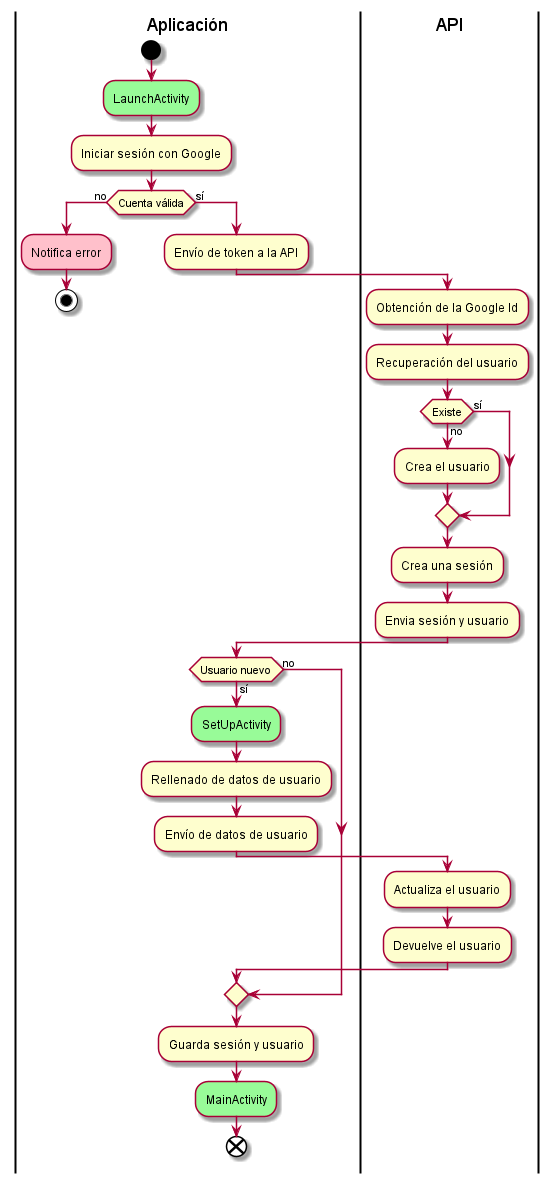
\includegraphics[width=0.65\textwidth]{images/Diseño/ActividadesInicioSesion.png}
    \caption{Diagrama de actividades del inicio de sesión}
    \label{dia:actividad_inicio_sesion}
\end{figure}

\begin{figure}
    \centering
    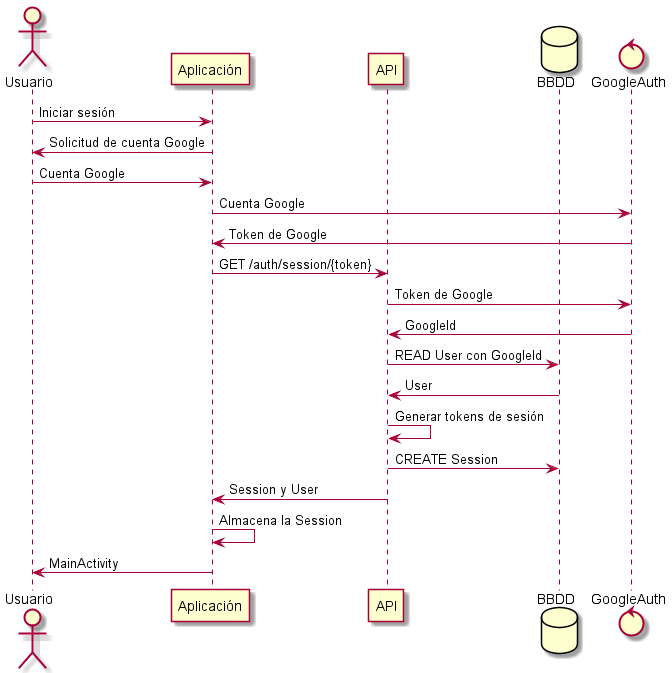
\includegraphics[width=0.5\textwidth]{images/Diseño/SecuenciaInicioSesion.png}
    \caption{Diagrama de secuencia del inicio de sesión}
    \label{dia:secuencia_inicio_sesion}
\end{figure}

\begin{figure}
    \centering
    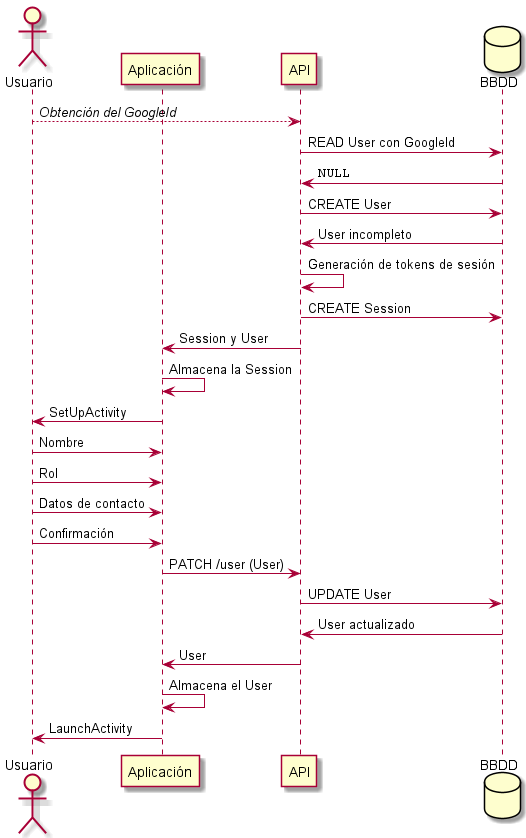
\includegraphics[width=0.5\textwidth]{images/Diseño/SecuenciaRegistro.png}
    \caption{Diagrama de secuencia de registro}
    \label{dia:secuencia_registro}
\end{figure}
\section{Vinculación}

\subsection{Creación de vínculos}

La vinculación de usuarios (relativa al 
\nameref{sec:cu:vinculacion}) es una función que requiere la participación activa de \textbf{dos actores}, un Paciente y un Cuidador. El proceso paralelo puede verse en la \fref{dia:actividad_vinculacion}, mientras que la secuencia pormenorizada de los procesos y comunicaciones entre componentes se muestra en la \fref{dia:secuencia_vinculacion}.

Este proceso se puede comprender como tres subprocesos: la generación del \gls{token} o código de vinculación, el escaneo de este y la validación del vínculo. El primero de ellos es el realizado por el Paciente al elegir la opción de \textbf{Añadir vínculo} en su pantalla de vínculos. Al hacerlo, su aplicación móvil emitirá una petición de \gls{token} al respectivo \gls{endpoint} (\fref{api:generar_token_vinculacion}) de la \acrshort{api}, que lo generará en base a los datos de dicho paciente y lo enviará como respuesta. Una vez que la aplicación móvil lo reciba, lo convertirá en un \textbf{código QR} y lo mostrará en la pantalla del Paciente. Estos códigos tendrá un tiempo de caducidad que también se enviará junto al código, si llega a caducar, la aplicación solicitará otro código y lo mostrará en la pantalla.

\begin{figure}[H]
    \centering
    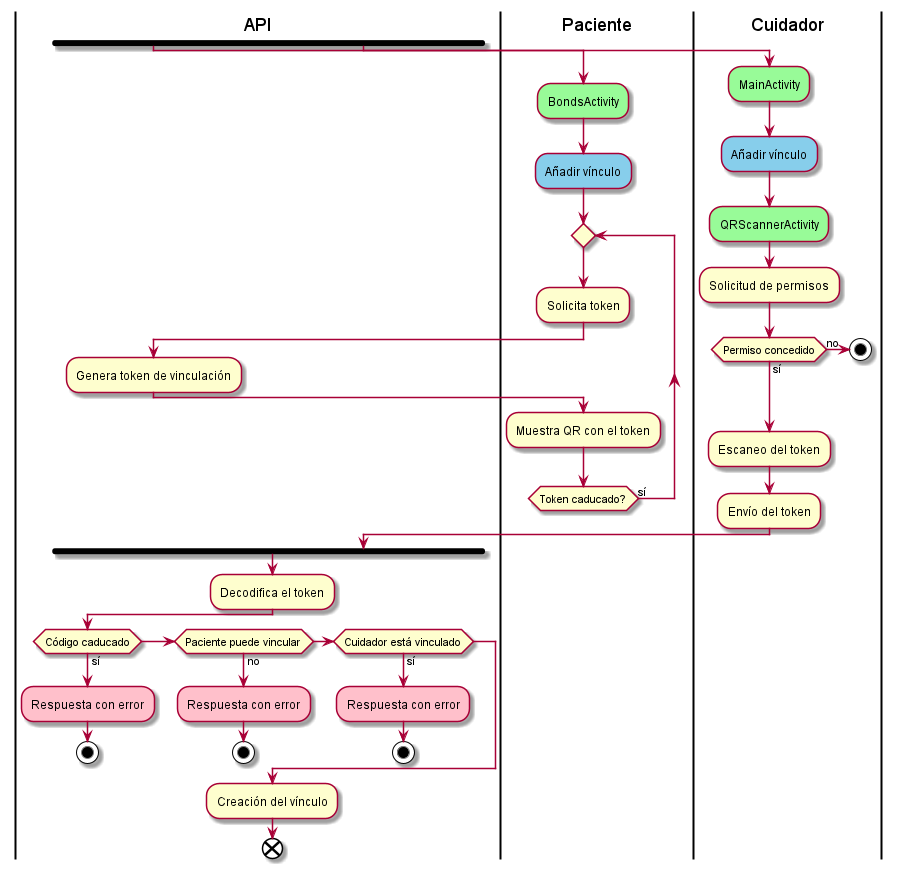
\includegraphics[width=0.7\textwidth]{images/Diseño/ActividadesVinculacion.png}
    \caption{Diagrama de actividades de la vinculación de usuarios}
    \label{dia:actividad_vinculacion}
\end{figure}

El Cuidador también iniciará su proceso por medio de una opción de \textbf{Añadir vínculo} situado en su pantalla principal. Al usarla la aplicación se dirigirá a la actividad del escáner y, previa obtención de requisitos de usuario, desde ella podrá enfocar el código QR mostrada en la aplicación del Paciente. La aplicación del Cuidador escaneará e \textbf{interpretará el código QR} obteniendo el \gls{token} que enviará a la \acrshort{api} con una petición al \gls{endpoint} del \fref{api:establecer_vinculo}.

\begin{figure}[H]
    \centering
    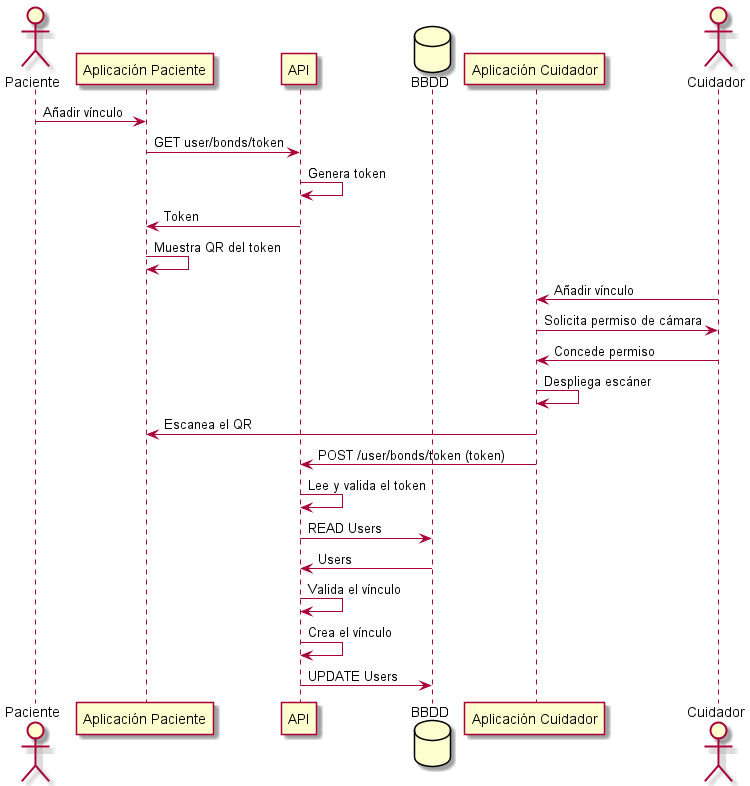
\includegraphics[width=0.5\textwidth]{images/Diseño/SecuenciaVinculacion.png}
    \caption{Diagrama de secuencia de la vinculación de usuarios}
    \label{dia:secuencia_vinculacion}
\end{figure}

Finalmente, una vez la \acrshort{api} reciba el \gls{token} del paciente comenzará su \textbf{lectura y validación}. Comprobará que el \gls{token} aún no haya caducado, si es el caso, lo leerá y obtendrá de él la ID del Paciente a vincular. Después solicitará la información de los usuarios para \textbf{comprobar si el vínculo es posible}. Si ese Paciente aún puede vincular más Cuidadores y el Cuidador no está vinculado, entonces la \acrshort{api} creará el vínculo añadiendo a cada uno de los actores a la lista de vínculos del otro, tras lo que actualizará los datos de ambos en la base de datos. De esta forma \textbf{el vínculo se habrá creado}.

\section{Ubicación}

El \textbf{\nameref{sec:cu:ubicacion}} trata acerca del envío de la ubicación actual del usuario al resto de sus usuarios asociados conectados a la misma sala de geolocalización. Un usuario se une a esta sala al acceder a la actividad de geolocalización, al hacerlo se envía un evento de suscripción a la WebSocket \acrshort{api}, que lo incluye en dicha sala.

\begin{figure}[H]
    \centering
    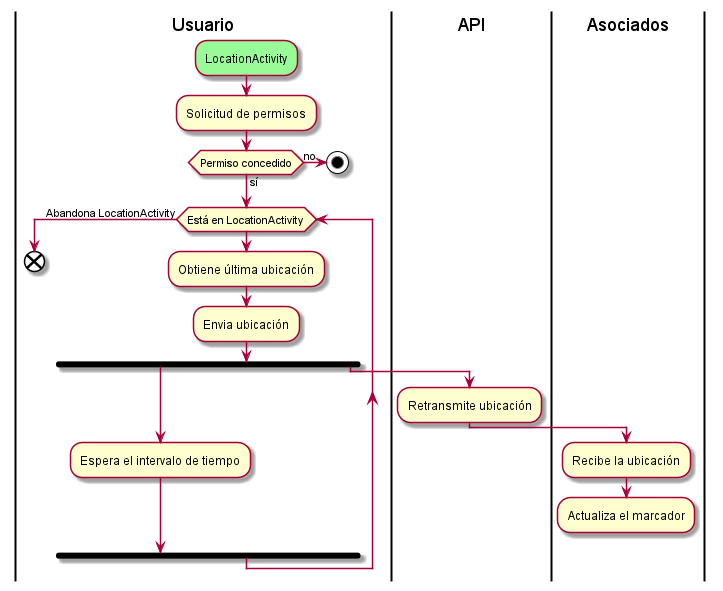
\includegraphics[width=0.5\textwidth]{images/Diseño/ActividadesUbicacion.png}
    \caption{Diagrama de actividades de la difusión de localizaciones}
    \label{dia:actividad_ubicacion}
\end{figure}

Para poder compartir la ubicación del usuario es necesario que este \textbf{conceda permisos} a la aplicación para poder usar los servicios de su dispositivo que la proporcionan. Una vez que lo haga, la aplicación mostrará al usuario una pantalla con un mapa y su localización además de la del resto de usuarios conectados, si hay alguno. En ese momento también se iniciará una tarea de fondo que de forma repetida tras un intervalo de tiempo \textbf{solicitará la última ubicación} del usuario y procederá a enviarla por el WebSocket a la \acrshort{api}.

\begin{figure}[H]
    \centering
    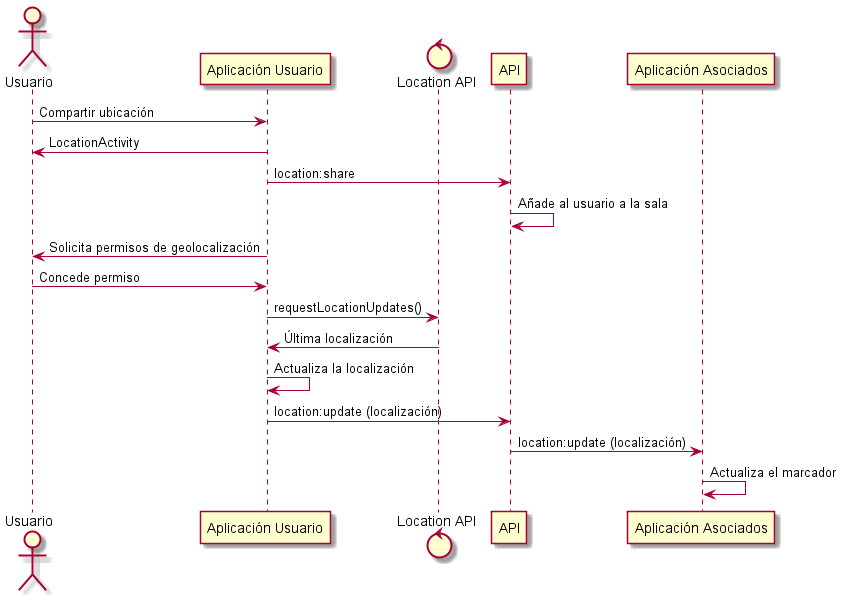
\includegraphics[width=0.7\textwidth]{images/Diseño/SecuenciaUbicacion.png}
    \caption{Diagrama de secuencia de la difusión de localizaciones}
    \label{dia:secuencia_ubicacion}
\end{figure}

La \acrshort{api} recibirá las ubicaciones de los usuario a través del evento de actualización (\fref{ws:location_update}), mismo evento que usará para \textbf{retransmitir esa ubicación} al resto de usuario conectados a dicha sala (pero no al emisor). Los usuarios asociados que estén compartiendo su ubicación recibirán la ubicación del usuario a través de dicho evento y actualizarán el marcador del mismo acorde a la nueva localización.
\subsection{Feed}

%feed:join
\begin{longtable}{|p{0.25\textwidth} p{0.75\textwidth}|}
    \hline
    \multicolumn{2}{|l|}{\textbf{FEED\textunderscore JOIN}} \\ \hline 
    Descripción         & Suscribe a un cliente a una sala de mensajería. \\ \hline
    Clave               & feed:join \\ \hline
    Tipo                & Retransmisión \\ \hline \hline
    Mensaje de entrada  &      
   \emph{object}. \acrshort{dto} con la información del usuario, del tipo \nameref{dto:usermin} (\fref{dto:usermin}). \\ \hline \hline
    Emisión   & FEED\textunderscore JOIN a los usuarios suscritos a la sala. \\ \hline \hline
    Errores     & Si el cliente no está conectado a una sala global .\\ \hline
    \caption{Documentación del evento Join de la sala Feed}
    \label{ws:feed_join}
\end{longtable}

%feed:leave
\begin{longtable}{|p{0.25\textwidth} p{0.75\textwidth}|}
    \hline
    \multicolumn{2}{|l|}{\textbf{FEED\textunderscore LEAVE}} \\ \hline 
    Descripción         & Da de baja a un cliente de su sala de mensajería. \\ \hline
    Clave               & feed:leave \\ \hline
    Tipo                & Retransmisión \\ \hline \hline
    Mensaje de entrada  &      
   \emph{object}. \acrshort{dto} con la información del usuario, del tipo \nameref{dto:usermin} (\fref{dto:usermin}). \\ \hline \hline
    Emisión
    & FEED\textunderscore LEAVE a los usuarios suscritos a la sala \\  \hline \hline
    Errores     & Si el cliente no está conectado a una sala de mensajería. \\ \hline
    \caption{Documentación del evento Leave de la sala Feed}
    \label{ws:feed_leave}
\end{longtable}

%feed:send
\begin{table}[H]
\begin{longtable}{|p{0.25\textwidth} p{0.75\textwidth}|}
    \hline
    \multicolumn{2}{|l|}{\textbf{FEED\textunderscore SEND}} \\ \hline 
    Descripción         & Envía un mensaje a través de la sala. \\ \hline
    Clave               & feed:send \\ \hline
    Tipo                & Cliente \\ \hline \hline
    Mensaje de entrada    &
   \emph{object}. \acrshort{dto} del mensaje, del tipo \nameref{dto:message} (\fref{dto:message}). \\ \hline \hline
    Emisión
    & FEED\textunderscore NEW a los usuarios suscritos a la sala \\ \hline \hline
    Errores     & Si el cliente no está conectado a una sala de mensajería \\ \hline
    \caption{Documentación del evento Send de la sala Feed}
    \label{ws:feed_send}
\end{longtable}
\end{table}

\newpage

%feed:new
\begin{longtable}{|p{0.25\textwidth} p{0.75\textwidth}|}
    \hline
    \multicolumn{2}{|l|}{\textbf{FEED\textunderscore NEW}} \\ \hline 
    Descripción         & Nuevo mensaje enviado a través de la sala. \\ \hline
    Clave               & feed:new \\ \hline
    Tipo                & Servidor \\ \hline \hline
    Emisión    &
   \emph{object}. \acrshort{dto} del mensaje, del tipo \nameref{dto:message} (\fref{dto:message}). \\ \hline
    \caption{Documentación del evento New de la sala Feed}
    \label{ws:feed_new}
\end{longtable}

%feed:delete
\begin{longtable}{|p{0.25\textwidth} p{0.75\textwidth}|}
    \hline
    \multicolumn{2}{|l|}{\textbf{FEED\textunderscore DELETE}} \\ \hline 
    Descripción         & Elimina un mensaje eviado a través de la sala. \\ \hline
    Clave               & feed:delete \\ \hline
    Tipo                & Servidor \\ \hline \hline
    Emisión    &
   \emph{object}. \acrshort{dto} del mensaje, del tipo \nameref{dto:message} (\fref{dto:message}). \\ \hline
    \caption{Documentación del evento Delete de la sala Feed}
    \label{ws:feed_delete}
\end{longtable}

\section{Notificaciones}

\subsection{Envío de notificaciones}

Cuando la \acrshort{api} procesa alguna de las acciones listadas en el \cref{req:notificaciones} genera una notificación. En la creación de esta notificación la \acrshort{api} busca en la base de datos los usuarios asociados y los añade como interesados a la entidad de la notificación antes de almacenarla en la base de datos de forma que pueda ser recuperada más adelante.

La notificación completa y devuelva por la base de datos es finalmente enviada por medio del WebSocket y el evento respectivo a la acción a notificar a los usuarios asociados, una vez recibida por las diferentes aplicaciones la muestran a sus usuarios por alguno de los medios dispuestos para tal hecho.

\begin{figure}[H]
    \centering
    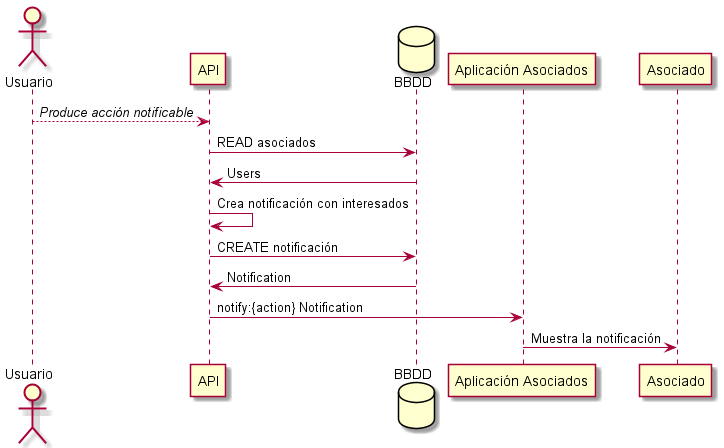
\includegraphics[width=0.75\textwidth]{images/Diseño/SecuenciaNotificaciones.png}
    \caption{Diagrama de secuencia del envío de notificaciones}
    \label{dia:secuencia_notificacion}
\end{figure}                 
\chapter{Interfaz de usuario}
\label{ch:diseño_interfaz_usuario}

\section{Guía de estilo}

A la hora de llevar a cabo el diseño de las interfaces de usuario se realizó una definición del estilo gráfico que tendría la aplicación y que se debería seguir para conseguir consistencia entre todas las pantallas de la misma. La base de la guía de estilo son \textbf{las directrices de Material Design} (véase \fref{ssec:guia_material_design}). Sobre esas bases se decidieron también los siguientes puntos:

\begin{itemize}
    \item El color principal de la aplicación será el \emph{dodger blue} (\code{\#29b6f6}).
    \item El color secundario de la aplicación será su complementario, el \emph{selective yellow} (\code{\#ffb300}).
    \item La aplicación ofrecerá temas claro y oscuro. Por defecto se mostrará acorde al tema del sistema operativo del usuario.
    \item Se utilizarán tarjetas para mostrar la información personal de los usuarios. 
    \begin{itemize}
        \item El nombre del usuario es la información mínima a mostrar inicialmente en la tarjeta.
        \item La información adicional de contacto estará en el anverso de la tarjeta o en una extensión desplegable, se usará la alternativa que más convenga a cada situación.
        \item Las dos alternativas se usarán con botones situados en el lado derecho de la tarjeta.
    \end{itemize}
    \item Todos los botones de navegación ofrecerán un icono y un texto indicando el destino.
    \item Los elementos de la interfaz como los botones o tarjetas tendrán bordes redondeados.
    \item Los errores se comunicarán por medio de \emph{toasts} al usuario.
    \item Todos los elementos utilizarán colores definidos en el tema de la aplicación.
\end{itemize}

\subsection{Tema de color}

El tema de color fue generado con la herramienta de que Material ofrece para tal empresa, \textbf{\nameref{ssec:color_tool}} (\fref{ssec:color_tool}), a partir de los dos colores que fueron seleccionados como colores base de la aplicación. La paleta de colores resultante fue la siguiente:

\begin{table}[H]
    \centering
    \begin{tabular}{|l|c|}  \hline
        \textbf{Color}         & \textbf{RGB} \\ \hline
        Primario         & \code{\#29b6f6} \\
        Primario claro         & \code{\#73e8ff} \\
        Primario oscuro        & \code{\#0086c3} \\ 
        Secundario         & \code{\#ffb300} \\ 
        Secundario claro         & \code{\#ffe54c} \\ 
        Secundario oscuro         & \code{\#c68400} \\ 
        Texto primario         & \code{\#000000} \\ 
        Texto secundario         & \code{\#212121} \\ 
        Superficie         & \code{\#eaf4f6} \\ \hline
    \end{tabular}
    \caption{Paleta de colores de la aplicación}
    \label{tab:paleta_colores}
\end{table}

\subsection{Icono de la aplicación}

El icono de la aplicación (\fref{fig:app_icon}) está basado en el lema principal y nombre de la aplicación, el \emph{"Todos para uno y uno para todos"},  que ya se comentó en el \fref{sec:justification}, y en el concepto de vínculos entre pacientes y cuidadores. 

El icono está compuesto por otros dos iconos que representan a su vez a los dos tipos de usuarios de la aplicación: los \textbf{Pacientes} (\fref{fig:patient_icon}) y los \textbf{Cuidadores} (\fref{fig:keeper_icon}). Los primeros son el punto central alrededor del que gira este sistema y su icono representa esto, un entidad central que recibe la ayuda exterior de sus cuidadores. Los Cuidadores por otro lado se representan como esas entidades exteriores que orbitan alrededor del Cuidador y que al hacerlo establecen vínculos entre sí, pues la base de esta aplicación radica también la cooperación entre Cuidadores. Los dos iconos superpuestos representan el entramado que se teje en \emph{All For One}, una cadena de socorro mutuo entre Pacientes y Cuidadores.

\vspace{30pt}
\begin{figure}[H]
    \centering
    \begin{minipage}{0.25\textwidth}
        \centering
        
\includegraphics[width=0.5\textwidth]{Diseño/patient-icon.png}
        \caption{Icono de Paciente}
        \label{fig:patient_icon}
    \end{minipage}\hfill
    \begin{minipage}{0.25\textwidth}
        \centering
        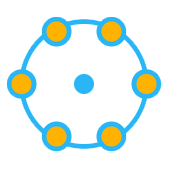
\includegraphics[width=0.5\textwidth]{Diseño/keeper-icon.png}
        \caption{Icono de Cuidador}
        \label{fig:keeper_icon}
    \end{minipage}\hfill
    \begin{minipage}{0.25\textwidth}
        \centering
        
\includegraphics[width=0.5\textwidth]{Diseño/4l1-icon.png}
        \caption{Icono de AllForOne}
        \label{fig:app_icon}
    \end{minipage}
\end{figure}

\section{Logo de la aplicación}

Además del icono también se creó un logo que permita identificar la aplicación de una forma más descriptiva y representativa, pues estará compuesto del nombre de la aplicación. La base de su diseño es el propio nombre de la aplicación y, por tanto, el lema de la misma. El logo (\fref{fig:app_logo}) es un \textbf{All} escrito con los colores del tema, los cuales distinguen también un \textbf{4} sobre la letra \emph{A} y un \textbf{1} bajo la letra \emph{L} del final. Esto nos deja: \textbf{ALL-4-1}, lo cuál leído en inglés tiene una lectura similar al nombre de la aplicación: \textbf{All For One.}

\begin{figure}[H]
    \centering
    
\includegraphics[width=0.5\textwidth]{images/Diseño/4l1-logo.png}
    \caption{Logo de la aplicación}
    \label{fig:app_logo}
\end{figure}

\section{Launch}

\begin{figure}[H]
    \centering
    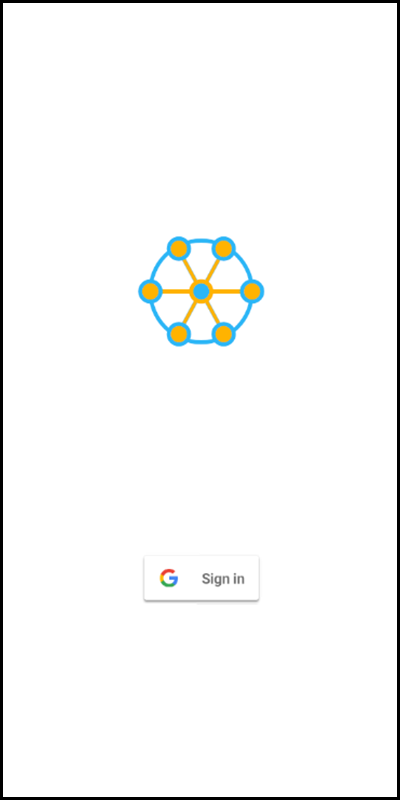
\includegraphics[width=0.25\textwidth]{Diseño/CapturaLaunch.png}
    \caption{Diseño de la pantalla de lanzamiento}
    \label{scr:launch}
\end{figure}

La pantalla de lanzamiento (\fref{scr:launch}) ofrece una única funcionalidad, \textbf{el inicio de sesión} con la cuenta de Google del usuario., por ello la pantalla contará únicamente con un botón para llevar a cabo esa acción. El botón en cuestión debe ser el servido por la propia biblioteca de autenticación de Google para ofrecer familiaridad al usuario y transmitir rápidamente que el inicio de sesión usa ese servicio. Aparte de dicho botón se dispondrá el icono de la aplicación para que el usuario sepa qué aplicación está empleando por si se inicia o accede a ella de forma indirecta. Hay margen para otros posibles añadidos como podrían ser la marca de registro o la versión de la aplicación.

\section{Set Up}

\begin{figure}[H]
    \centering
    \begin{minipage}{0.20\textwidth}
        \centering
        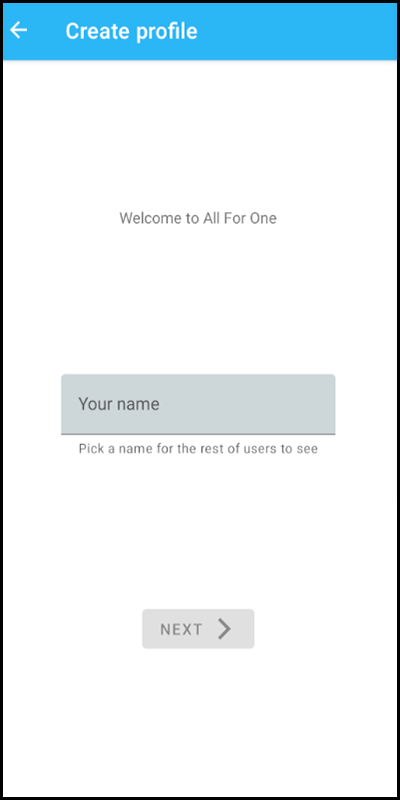
\includegraphics[width=1\textwidth]{Diseño/CapturaSetUpA.png}
        \caption{Diseño de la pantalla de configuración de nombre}
        \label{scr:setup_name}
    \end{minipage}\hfill
    \begin{minipage}{0.20\textwidth}
        \vspace{-18pt}
        \centering
        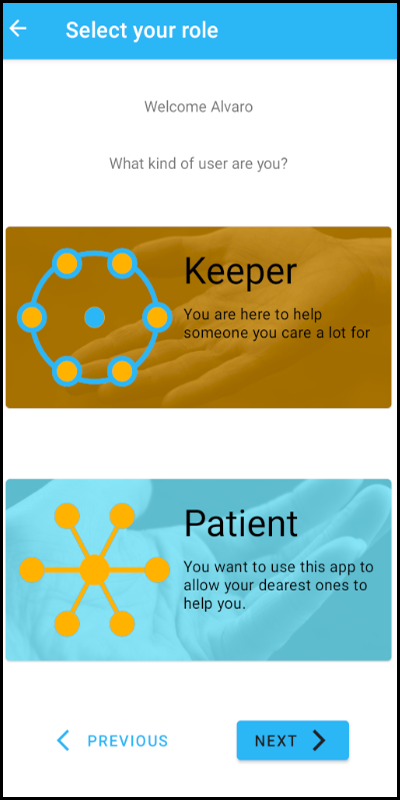
\includegraphics[width=1\textwidth]{Diseño/CapturaSetUpB.png}
        \caption{Diseño de la pantalla de elección de rol}
        \label{scr:setup_role}
    \end{minipage}\hfill
    \begin{minipage}{0.20\textwidth}
        \centering
        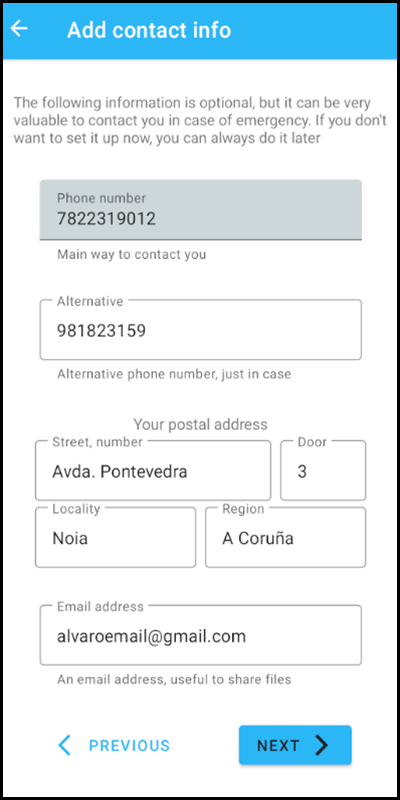
\includegraphics[width=1\textwidth]{Diseño/CapturaSetUpC.png}
        \caption{Diseño de la pantalla de introducción de datos}
        \label{scr:setup_contact}
    \end{minipage}\hfill
    \begin{minipage}{0.20\textwidth}
        \centering
        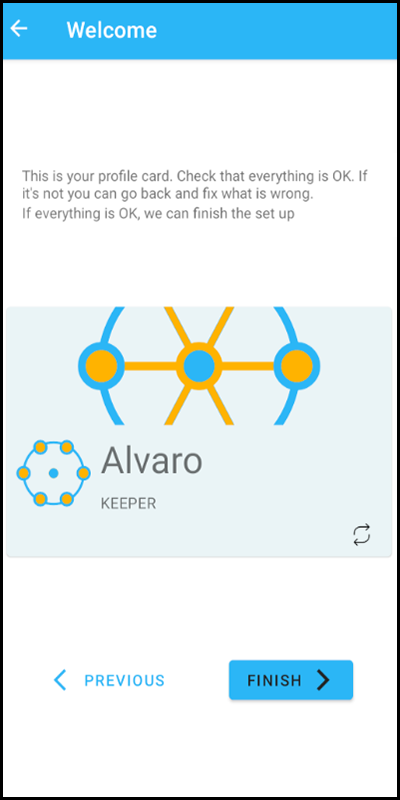
\includegraphics[width=1\textwidth]{Diseño/CapturaSetUpD.png}
        \caption{Diseño de la pantalla de confirmación del perfil}
        \label{scr:setup_confirmation}
    \end{minipage}\hfill
\end{figure}

La pantalla de configuración del perfil será la pantalla a la que accedan los nuevos usuarios que intenten iniciar sesión por primera vez. Esta pantalla estará compuesta por cuatro distintas, una para cada etapa del proceso con tendrán botones para avanzar o retroceder entre ellas. 

La primera de estas pantallas es la de \textbf{configuración del nombre} (\fref{scr:setup_name}), donde habrá un campo de texto en el que el usuario podrá introducir el nombre que lo represente. A esta pantalla le sigue la de \textbf{selección del rol} ( \fref{scr:setup_role}), que ofrecerá dos tarjetas representando las opciones.

Una vez seleccionado el rol, el usuario progresará a otra pantalla (\fref{scr:setup_contact}) donde podrá rellenar sus \textbf{datos de contacto} en los distintos campos de texto que se le dispondrán para tal acción. Tras completar todos estos pasos la única pantalla restante será la de \textbf{confirmación del perfil} (\fref{scr:setup_confirmation}). En esta última pantalla se mostrará la tarjeta de perfil del usuario con los datos que ha introducido de forma que pueda ver todo de nuevo de forma sencilla antes de terminar el registro.

\section{Main}

\begin{figure}[H]
    \centering
    \begin{minipage}{0.5\textwidth}
        \centering
        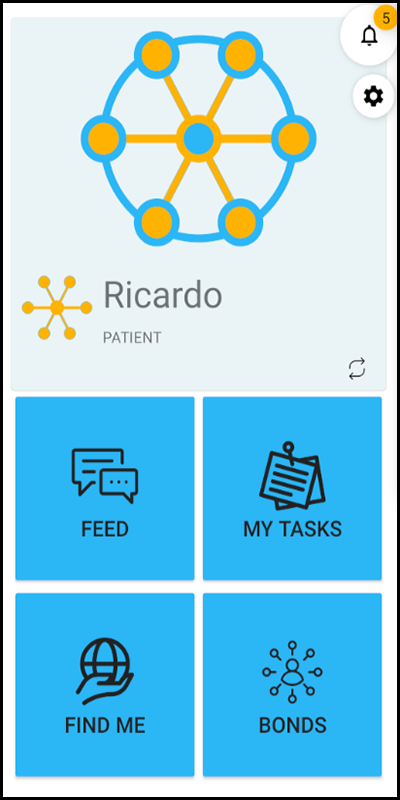
\includegraphics[width=0.5\textwidth]{Diseño/CapturaMainA.png}
        \label{scr:main}
    \end{minipage}\hfill
    \begin{minipage}{0.5\textwidth}
        \centering
        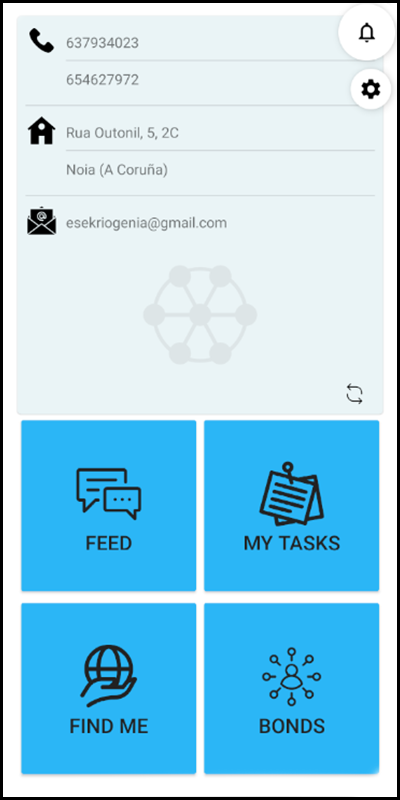
\includegraphics[width=0.5\textwidth]{Diseño/CapturaMainB.png}
        \label{scr:main_b}
    \end{minipage}\hfill
    \caption{Diseño de la pantalla principal}
\end{figure}

La pantalla principal es el punto de navegación principal de la aplicación y da acceso al resto de funciones de la aplicación. Al ser el también el punto de entrada tras el inicio de sesión es un lugar idóneo para situar \textbf{los datos del Paciente}, de forma que el acceso a los mismos requiera el menor esfuerzo posible de memoria, facilitando el acceso a ellos a los usuarios con los síntomas de la enfermedad. La tarjeta es voltaeable por medio del botón situado en su esquina inferior derecha.

Las cuatro grandes funciones principales de la aplicación (el feed de comunicación, la gestión de tareas, la geolocalización y la consulta de vínculos) serán accesibles a través de los \textbf{cuatros grandes botones} situados bajo la tarjeta del Paciente. Al ser las funciones principales cuenta con un acceso más resaltable que los demás puntos de navegación de la pantalla.

Esos otros dos puntos de navegación son el acceso a las notificaciones y a los ajustes. Los botones a los mismos no cuentan con el relleno del color principal y están situados en la esquina superior derecha, lugar habitual de localización para estas funciones. El acceso a las notificaciones contará además con una chapa indicando \textbf{el número de notificaciones} no leídas que tiene el usuario, indicando así si es necesario desplegar dicha pantalla.

\section{Feed}

\begin{figure}[H]
    \centering
    \begin{minipage}{0.5\textwidth}
        \centering
        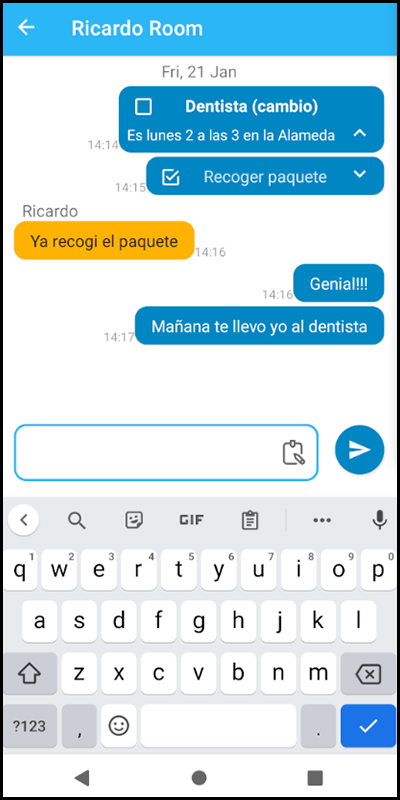
\includegraphics[width=0.5\textwidth]{Diseño/CapturaFeed.png}
        \label{scr:feed}
    \end{minipage}\hfill
    \begin{minipage}{0.5\textwidth}
        \centering
        \includegraphics[width=0.5\textwidth]{Diseño/CapturaFeedTarea.png}
        \label{scr:feed_task_mode}
    \end{minipage}\hfill
    \caption{Diseño de la pantalla de feed}
\end{figure}

El diseño de la pantalla del feed (\fref{scr:feed}) es similar a los diseños habituales de \textbf{pantallas de chat}. En el lado derecho y en azul se mostrarán los mensajes usados por el propio usuario y a la izquierda se listarán los mensajes enviados por los usuarios asociados con el nombre del usuario que lo envió. Como en los diseños habituales, en la parte inferior se ofrecerá un campo de texto para escribir y enviar el mensaje con el botón de su derecha.

Todos los mensajes mostrarán la hora de envío de los mismos y se agruparán por fecha de envío. Las tareas se mostrarán como mensajes de texto pero incluyendo además una casilla representando su estado y una flecha que permita desplegar la descripción de la tarea. Las tareas ya completas se verán con un color de texto más apagado para que sean fácilmente distinguibles a primera vista.

Una diferencia que tendrá esta pantalla de feed respecto a otros chats será el \textbf{modo crear tarea}. Este se mostrará usando el botón con forma de portafolios del interior del campo de texto. Al usarlo el icono cambiará a una X que sirva para cerrarlo y una campo de texto mayor se abrirá en la parte inferior de la pantalla para poder introducir la descripción. El envío de estas será con el mismo botón que los mensajes de texto.

\section{Tasks}

\begin{figure}[H]
    \centering
    \begin{minipage}{0.45\textwidth}
        \centering
        \includegraphics[width=0.5\textwidth]{Diseño/CapturaTareas.png}
        \caption{Diseño de la pantalla de tareas}
        \label{scr:task}
    \end{minipage}\hfill
    \begin{minipage}{0.45\textwidth}
        \centering
        \includegraphics[width=0.5\textwidth]{Diseño/CapturaTareasCrear.png}
        \caption{Diseño de la pantalla de crear tarea}
        \label{scr:task_crear}
    \end{minipage}\hfill
\end{figure}

La pantalla de tareas (\fref{scr:task}) lista las tareas en tarjetas con el título, una casilla con el estado de la tarea, el autor de la misma y la fecha de creación de la tarea. Más información como la descripción o el último momento de actualización se mostrarán al desplegar los datos de la tarea con la flecha de la tarjeta para tal uso. Las tareas ya completas tendrán color y texto más claro, por lo que a simple vista \textbf{podrán diferenciarse los dos tipos de tarea}. La casilla del estado será también un botón que se pueda usar para cambiar el estado de la tarea, además de este botón habrá otro para eliminarlas. 

Finalmente, la pantalla también tendrá un botón para desplegar la pantalla de \textbf{creación de tareas} (\fref{scr:task_crear}). En dicho diálogo habrá un campo de texto para introducir el título y otro para rellenar la descripción. La creación de la tarea se podrá confirmar o cancelar con los botones que este diálogo tendrá en la parte inferior.

\section{Location}

\begin{figure}[H]
    \centering
    \includegraphics[width=0.2\textwidth]{Diseño/CapturaLocalización.png}
    \caption{Diseño de la pantalla de geolocalización}
    \label{scr:location}
\end{figure}

La pantalla de geolocalización (\fref{scr:location}) es una \textbf{actividad con un mapa} que ocupa toda la actividad similar a muchos otros servicios. Los colores del mapa de Google Maps se ofrecerán modificados para que vayan más acordes a los colores de la aplicación. En esa pantalla se mostrará la posición del usuario con un círculo azul con un cono visión. Marcadores de distintos colores representarán las posiciones del resto de usuarios asociados conectados. Pulsar en esos marcadores mostrará el nombre del usuario al que pertenece.

\section{Bonds}

\begin{figure}[H]
    \centering
    \begin{minipage}{0.5\textwidth}
        \centering
        \includegraphics[width=0.45\textwidth]{Diseño/CapturaBondList.png}
        \label{scr:bonds}
    \end{minipage}\hfill
    \begin{minipage}{0.5\textwidth}
        \centering
        \includegraphics[width=0.45\textwidth]{Diseño/CapturaBoundB.png}
        \label{scr:bonds_qr}
    \end{minipage}\hfill
    \caption{Diseño de la pantalla de vínculos}
\end{figure}

La función de acceso a los vínculos se servirá en una pantalla (\fref{scr:bonds}) que listará los vínculos. Cada uno de estos vínculos \textbf{será una tarjeta} con el nombre del usuario que podrá ser desplegada para mostrar los datos de contacto. Los pacientes, además, tendrán un botón en la parte inferior que les permitirá desplegar un nuevo código QR con un \gls{token} de vinculación como se puede ver en \fref{scr:bonds_qr}.

\section{Scanner}

\begin{figure}[H]
    \centering
    \begin{minipage}{0.45\textwidth}
        \centering
        \includegraphics[width=0.5\textwidth]{Diseño/CapturaBoundA.png}
        \caption{Diseño de la pantalla principal sin vínculo}
        \label{scr:unbonded}
    \end{minipage}\hfill
    \begin{minipage}{0.45\textwidth}
        \centering
        \includegraphics[width=0.5\textwidth]{Diseño/CapturaScanner.png}
        \caption{Diseño de la pantalla de escáner}
        \label{scr:scanner}
    \end{minipage}\hfill
\end{figure}

Para completar los vínculos se debe escanear el código QR, lo que se hace en la pantalla de escáner (\fref{scr:scanner}) a la que se podrán acceder los \textbf{Cuidadores no vinculados} a través de su actividad principal, que se mostrará como se ve en \fref{scr:unbonded}, con únicamente un botón para abrir el escáner. El susodicho escáner será una pantalla ocupada por completo por la cámara en la que estará oscurecida la sección en la que no podrá enfocarse el código.

\section{Notifications}

Las notificaciones se desplegarán y mostrarán en una pantalla como la mostrada en \fref{scr:notifications}. Dicha pantalla listará las acciones a notificar agrupadas según la fecha en la que sucedieron y en un orden de más recientes a más antiguas. Cada notificará contará con un botón con el icono de un ojo para marcar esa notificación como vista. Aparte de ese botón habrá otro en la parte superior para \textbf{marcar todas como vistas}. Por último, las notificaciones relacionadas con alguna pantalla o acceso que se deba visitar contarán con un botón para navegar hasta dicho lugar de la aplicación.



\begin{figure}[H]
    \centering
    \begin{minipage}{0.4\textwidth}
        \centering
        \includegraphics[width=0.5\textwidth]{Diseño/CapturaNotificaciones.png}
        \caption{Diseño de la pantalla de notificaciones}
        \label{scr:notifications}
    \end{minipage}\hfill
    \begin{minipage}{0.4\textwidth}
        \centering
        \includegraphics[width=0.5\textwidth]{Diseño/CapturaAjustes.png}
        \caption{Diseño de la pantalla de ajustes}
        \label{scr:settings}
    \end{minipage}\hfill
\end{figure}

\section{Settings}

Las opciones, al igual que las notificaciones, será un diálogo a pantalla completa que se abrirá desde la pantalla principal. Será como la \fref{scr:settings}. En esta pantalla se listarán las posibles opciones del usuario. La opción de \textbf{editar usuario} desplegará campos de texto de las diferentes propiedades del usuario para que este pueda editarlas, lo cuál confirmará con un botón que también se desplegará con la misma opción. El resto de opciones serán también botones, y habrá uno más para cerrar el diálogo y retornar a la pantalla principal.

\section{Mapa de navegación}

El mapa de navegación definitivo con las pantallas recién mostradas es el ilustrado en \fref{scr:navigation}. Las pantallas con fondo azul requieren inicio de sesión y las que tienen fondo verde son exclusivas de los Cuidadores no vinculados.

La navegación comienza siempre en LaunchActivity. Si el usuario no está registrado avanzará a SetUpActivity a través de sus cuatro fragmentos en orden. Si está registrado o si completa el registro a través de SetUpActivity avanzará a MainActivity, desde donde se navegarán al resto de actividades y a los diálogos de notificaciones y ajustes. 

Se ha intentando reducir los pasos de navegación al mínimo y por ello prácticamente todas las funcionalidades son accesibles con una única navegación desde la pantalla principal. A excepción del diálogo de crear tarea, que debe accederse desde TasksActivity.

\begin{figure}[H]
    \centering
    \includegraphics[width=1\textwidth]{Diseño/MapaNavegacionDiseño.drawio.png}
    \caption{Mapa de navegación}
    \label{scr:navigation}
\end{figure}                     
\chapter{Especificación técnica del plan de pruebas}
\label{ch:especificacion_tecnica_plan_pruebas}

\section{Pruebas unitarias}
\subsection{Aplicación móvil}

\begin{longtable}{ l l c }
    \hline
    Referencia & Caso & Resultado \\
    \hline
    \ref{cp:u:app:actualizar_datos} & Actualizar datos del usuario & NO \\
    \ref{cp:u:app:cerrar_sesion_usuario} & Cerrar la sesión de usuario & NO \\
    \ref{cp:u:app:eliminar_vinculo} & Eliminar el vínculo con el Paciente vinculado & NO \\ \hline
    \ref{cp:u:app:añadir_marcador} & Añadir un marcador & PASA \\
    \ref{cp:u:app:comprobar_marcador} & Comprobar la existencia de un marcador & PASA \\
    \ref{cp:u:app:eliminar_marcador} & Eliminar un marcador & PASA \\
    \ref{cp:u:app:actualizar_marcador} & Actualizar un marcador & PASA \\ \hline
    \ref{cp:u:app:añadir_notificacion} & Añadir una notificación & NO \\
    \ref{cp:u:app:añadir_conjunto_notificaciones} & Añadir un conjunto de notificaciones & NO \\
    \ref{cp:u:app:limpiar_lista_notificaciones} & Limpiar lista de notificaciones & NO \\
    \ref{cp:u:app:cargar_lista_notificaciones} & Cargar lista de notificaciones & NO \\
    \ref{cp:u:app:eliminar_notificacion} & Eliminar una notificación & NO \\
    \ref{cp:u:app:eliminar_todas_notificaciones} & Eliminar todas las notificaciones & NO \\ \hline
    \ref{cp:u:app:enviar_confirmacion_datos_usuario} & Enviar confirmación de datos de usuario & PASA \\
    \ref{cp:u:app:gestionar_resultado_inicio_google} & Gestionar resultado de inicio de sesión en Google & PASA \\
    \ref{cp:u:app:gestionar_resultado_inicio_google_erroneo} & Gestionar resultado de inicio de sesión en Google erróneo & PASA \\ \hline
    \ref{cp:u:app:añadir_nuevo_marcador_vista} & Añadir un nuevo marcador & PASA \\
    \ref{cp:u:app:recibir_actualizacion_posicion_no_existente} & Recibir una actualización de posición de marcador no existente & NO \\
    \ref{cp:u:app:recibir_actualizacion_posicion_marcador} & Recibir una actualización de posición de marcador ya existente & NO \\ \hline  
    \ref{cp:u:app:obtener_pagina_mensajes} & Obtener una página de mensajes & PASA \\
    \ref{cp:u:app:enviar_tarea_feed} & Enviar una tarea por el feed & NO \\
    \ref{cp:u:app:enviar_mensaje_feed} & Enviar un mensaje por el feed & NO \\
    \ref{cp:u:app:recibir_actualizacion_tarea} & Recibir una actualización de tarea & NO \\
    \ref{cp:u:app:recibir_eliminacion_tarea} & Recibir una eliminación de tarea & NO \\
    \ref{cp:u:app:recibir_nuevo_mensaje} & Recibir un nuevo mensaje & NO \\ \hline
    \caption{Primera parte de los resultados de las pruebas unitarias de la aplicación}
\end{longtable}   

\begin{figure}[H]
\begin{longtable}{ l l c }
    \hline
    Referencia & Caso & Resultado \\
    \hline    
    \ref{cp:u:app:confirmar_creacion_tarea} & Confirmar creación de una tarea & PASA \\
    \ref{cp:u:app:eliminacion_tarea_vista} & Eliminación una tarea & PASA \\
    \ref{cp:u:app:eliminacion_tarea_invalida} & Eliminación una tarea inválida & PASA \\
    \ref{cp:u:app:marcar_tarea_hecha_no_hecha} & Marcar tarea como hecha/no hecha & PASA \\
    \ref{cp:u:app:obtener_lista_tareas} & Obtener la lista de tareas & PASA \\ \hline
    \ref{cp:u:app:eliminar_vinculo_vista} & Eliminar un vínculo & NO \\
    \ref{cp:u:app:obtener_codigo_qr_vinculacion} & Obtener un código QR de vinculación & NO \\
    \ref{cp:u:app:obtener_vinulos_vista} & Obtener los vínculos & PASA \\ \hline
    \ref{cp:u:app:actualizar_usuario_vista} & Actualizar usuario & NO \\
    \ref{cp:u:app:enviar_codigo_vinculacion_vista} & Enviar código de vinculación & PASA \\
    \ref{cp:u:app:obtener_lista_notificaciones_vista} & Obtener lista de notificaciones & NO \\
    \ref{cp:u:app:obtener_paciente_vinculado_vista} & Obtener Paciente vinculado & PASA \\ \hline
    \ref{cp:u:app:envio_mensajes_repo} & Envío de mensaje & NO \\
    \ref{cp:u:app:recuperacion_mensajes_repo} & Recuperación de mensajes & PASA \\ \hline
    \ref{cp:u:app:recuperacion_notificaciones_repo} & Recuperación de notificaciones & PASA \\
    \ref{cp:u:app:marcado_notificacion_leida_repo} & Marcado de notificación como leída & PASA \\
    \ref{cp:u:app:marcado_todas_notificaciones_leidas_repo} & Marcado de todas las notificaciones como leídas & PASA \\ \hline
    \ref{cp:u:app:inicio_sesion_repo} & Inicio de sesión & PASA \\
    \ref{cp:u:app:cierre_sesion_repo} & Cierre de sesión & PASA \\
    \ref{cp:u:app:refresco_sesion_repo} & Refresco de sesión & PASA \\
    \ref{cp:u:app:recuperacion_tareas_repo} & Recuperación de tareas & PASA \\
    \ref{cp:u:app:guardado_tarea_repo} & Guardado de una tarea & PASA \\
    \ref{cp:u:app:eliminacion_tarea_repo} & Eliminación de una tarea & PASA \\
    \ref{cp:u:app:actualizacion_tarea_repo} & Actualización de una tarea & PASA \\ \hline
    \ref{cp:u:app:actualizacion_usuario_repo} & Actualización de un usuario & PASA \\
    \ref{cp:u:app:eliminar_vinculacion_repo} & Eliminar vinculación & PASA \\
    \ref{cp:u:app:enviar_codigo_vinculacion_repo} & Enviar código de vinculación & PASA \\
    \ref{cp:u:app:recuperacion_vinculos_repo} & Recuperación de vínculos & PASA \\
    \ref{cp:u:app:recuperacion_paciente_repo} & Recuperación del Paciente vinculado & PASA \\
    \ref{cp:u:app:solicitar_codigo_vinculacion_repo} & Solicitar código de vinculación & PASA \\ \hline
    \ref{cp:u:app:obtencion_servicio} & Obtención de un servicio & PASA \\ \hline
    \ref{cp:u:app:respuesta_inicio_sesion} & Procesar respuesta de inicio de sesión & PASA \\
    \ref{cp:u:app:respuesta_refresco_sesion} & Procesar respuesta de refresco de sesión & PASA \\ \hline
    \ref{cp:u:app:respuesta_recuperacion_notificaciones} & Procesar respuesta de recuperación de notificaciones & PASA \\
    \ref{cp:u:app:respuesta_recuperacion_mensajes} & Procesar respuesta de recuperación de mensajes & PASA \\ \hline
    \caption{Segunda parte de los resultados de las pruebas unitarias de la aplicación}
\end{longtable}   
\end{figure}    

\begin{figure}[H]
\begin{longtable}{ l l c }
    \hline
    Referencia & Caso & Resultado \\
    \hline  
    \ref{cp:u:app:respuesta_recuperacion_tareas} & Procesar respuesta de recuperación de tareas & PASA \\
    \ref{cp:u:app:respuesta_publicacion_tareas} & Procesar respuesta de publicación de tareas & PASA \\ \hline
    \ref{cp:u:app:respuesta_actualizacion_usuario} & Procesar respuesta de actualización de usuario & PASA \\
    \ref{cp:u:app:respuesta_recuperacion_paciente_vinculado} & Procesar respuesta de recuperación de Paciente vinculado & PASA \\
    \ref{cp:u:app:respuesta_recuperacion_vinculos} & Procesar respuesta de recuperación de vínculos & PASA \\
    \ref{cp:u:app:respuesta_recuperacion_codigo_vinculacion} & Procesar respuesta de recuperación de código de vinculación & PASA \\ \hline
    \caption{Tercera parte de los resultados de las pruebas unitarias de la aplicación}
\end{longtable}  
\end{figure} 

En el desarrollo de pruebas de la aplicación no fueron posibles realizar todas las pruebas que estaban planeadas por limitaciones de tiempo. Dentro de las que sí pudieron implementadas se consiguió un éxito completo. Estas pruebas necesitan mayor trabajo.
\subsection{API}

\subsubsection{Middleware de autenticación}

\begin{longtable}{|p{0.25\textwidth} p{0.75\textwidth}|}
    \hline
    \multicolumn{2}{|l|}{\textbf{Encabezado de autenticación correcto}} \\ \hline 
    Descripción                 & Se lanza una petición privada con un encabezado de autenticación con formato y token correctos \\ \hline
    Entrada                     & Petición con encabezado "Authorization: Bearer valid" \\ \hline
    Resultado esperado          & Extrae el token y llama a la siguiente función \\ \hline
    \caption{Prueba unitaria de la API: Encabezado de autenticación correcto}
    \label{cp:u:api:encabezado_correcto}
\end{longtable}

\begin{longtable}{|p{0.25\textwidth} p{0.75\textwidth}|}
    \hline
    \multicolumn{2}{|l|}{\textbf{Encabezado de autenticación faltante}} \\ \hline 
    Descripción                 & Se lanza una petición privada sin encabezado de autenticación \\ \hline
    Entrada                     & Petición sin encabezado de autorización \\ \hline
    Resultado esperado          & Error Bad Request \\ \hline
    \caption{Prueba unitaria de la API: Encabezado de autenticación faltante}
    \label{cp:u:api:encabezado_faltante}
\end{longtable}

\begin{longtable}{|p{0.25\textwidth} p{0.75\textwidth}|}
    \hline
    \multicolumn{2}{|l|}{\textbf{Encabezado de autenticación mal formateado}} \\ \hline 
    Descripción                 & Se lanza una petición privada con encabezado de autenticación con formato erróneo \\ \hline
    Entrada                     & Petición con encabezado sin Bearer \\ 
                                & Petición con encabezado con Bearer mal escrito \\ \hline
    Resultado esperado          & Error Bad Request \\ \hline
    \caption{Prueba unitaria de la API: Encabezado de autenticación mal formateado}
    \label{cp:u:api:encabezado_mal_formateado}
\end{longtable}

\begin{longtable}{|p{0.25\textwidth} p{0.75\textwidth}|}
    \hline
    \multicolumn{2}{|l|}{\textbf{Encabezado de autenticación con token inválido}} \\ \hline 
    Descripción                 & Se lanza una petición privada con encabezado de autenticación con formato erróneo \\ \hline
    Entrada                     & Petición con encabezado "Authorization: Bearer invalid" \\ \hline
    Resultado esperado          & Error Unauthorized \\ \hline
    \caption{Prueba unitaria de la API: Encabezado de autenticación con token inválido}
    \label{cp:u:api:encabezado_token_invalido}
\end{longtable}

\vspace{-20pt}
\subsubsection{Middleware de manejo de errores}

\begin{longtable}{|p{0.25\textwidth} p{0.75\textwidth}|}
    \hline
    \multicolumn{2}{|l|}{\textbf{Manejo correcto de errores conocidos}} \\ \hline 
    Descripción                 & Se lanza un error HTTP esperando la respuesta correspondiente \\ \hline
    Entrada                     & HttpError con diferentes estados \\ \hline
    Resultado esperado          & Respuesta de error con el estado del error lanzado \\ \hline
    \caption{Prueba unitaria de la API: Manejo correcto de errores conocidos}
    \label{cp:u:api:manejo_error_correcto}
\end{longtable}

\vspace{-15pt}
\begin{longtable}{|p{0.25\textwidth} p{0.75\textwidth}|}
    \hline
    \multicolumn{2}{|l|}{\textbf{Manejo correcto de errores desconocidos}} \\ \hline 
    Descripción                 & Se lanza un Error esperando una respuesta de error interno \\ \hline
    Entrada                     & Error \\ \hline
    Resultado esperado          & Respuesta con estado 500: Internal Server Error \\ \hline
    \caption{Prueba unitaria de la API: Manejo correcto de errores desconocidos}
    \label{cp:u:api:manejo_correcto_desconocido}
\end{longtable}

\vspace{-20pt}
\subsubsection{Servicio de mensajes}

\begin{longtable}{|p{0.25\textwidth} p{0.75\textwidth}|}
    \hline
    \multicolumn{2}{|l|}{\textbf{Creación de un mensaje de texto}} \\ \hline 
    Descripción                 & Se persiste un mensaje de texto válido en la base de datos \\ \hline
    Entrada                     & Mensaje de texto válido \\ \hline
    Resultado esperado          & Mensaje persistido en la base de datos \\
                                & Retorno del mensaje creado \\ \hline
    \caption{Prueba unitaria de la API: Creación de un mensaje de texto}
    \label{cp:u:api:crear_mensaje_texto}
\end{longtable}

\vspace{-15pt}
\begin{longtable}{|p{0.25\textwidth} p{0.75\textwidth}|}
    \hline
    \multicolumn{2}{|l|}{\textbf{Creación de un mensaje de texto inválido}} \\ \hline 
    Descripción                 & Se persiste un mensaje de texto inválido en la base de datos \\ \hline
    Entrada                     & Mensaje de texto sin alguna propiedad obligatoria \\ \hline
    Resultado esperado          & HttpError con BadRequest \\ \hline
    \caption{Prueba unitaria de la API: Creación de un mensaje de texto inválido}
    \label{cp:u:api:crear_mensaje_texto_invalido}
\end{longtable}

\begin{longtable}{|p{0.25\textwidth} p{0.75\textwidth}|}
    \hline
    \multicolumn{2}{|l|}{\textbf{Recuperación de mensajes}} \\ \hline 
    Descripción                 & Se recupera la primera página de mensajes de una habitación \\ \hline
    Entrada                     & Habitación de los mensajes \\ \hline
    Resultado esperado          & Lista de mensajes esperados \\ \hline
    \caption{Prueba unitaria de la API: Recuperación de mensajes}
    \label{cp:u:api:recuperar_mensaje}
\end{longtable}

\begin{longtable}{|p{0.25\textwidth} p{0.75\textwidth}|}
    \hline
    \multicolumn{2}{|l|}{\textbf{Recuperación de mensajes de una página concreta}} \\ \hline 
    Descripción                 & Se recupera una página de mensajes de una habitación distinta de la primera \\ \hline
    Entrada                     & Habitación de los mensajes y página a recuperar \\ \hline
    Resultado esperado          & Lista de mensajes esperados \\ \hline
    \caption{Prueba unitaria de la API: Recuperación de mensajes de una página concreta}
    \label{cp:u:api:recuperar_mensaje_pagina}
\end{longtable}

\subsubsection{Servicio de notificaciones}

\begin{longtable}{|p{0.25\textwidth} p{0.75\textwidth}|}
    \hline
    \multicolumn{2}{|l|}{\textbf{Creación de una notificación}} \\ \hline 
    Descripción                 & Se crea y persiste una notificación en la base de datos \\ \hline
    Entrada                     & Acción e ID del autor \\ \hline
    Resultado esperado          & Notificación persistida en la base de datos \\
                                & Retorno de la notificación creada \\ \hline
    \caption{Prueba unitaria de la API: Creación de una notificación}
    \label{cp:u:api:crear_notificacion}
\end{longtable}

\begin{longtable}{|p{0.25\textwidth} p{0.75\textwidth}|}
    \hline
    \multicolumn{2}{|l|}{\textbf{Marcado de una notificación con más interesados como leída}} \\ \hline 
    Descripción                 & Se marcan una notificación con más interesados como leída por un usuario \\ \hline
    Entrada                     & ID de la notificación y del usuario \\ \hline
    Resultado esperado          & La notificación es marcada como leída por el usuario \\ \hline
    \caption{Prueba unitaria de la API: Marcado de una notificación con más interesados como leída}
    \label{cp:u:api:marcar_notificacion_leida}
\end{longtable}

\newpage
\begin{longtable}{|p{0.25\textwidth} p{0.75\textwidth}|}
    \hline
    \multicolumn{2}{|l|}{\textbf{Marcado de una notificación sin más interesados como leída}} \\ \hline 
    Descripción                 & Se marcan una notificación sin más interesados como leída por el usuario \\ \hline
    Entrada                     & ID de la notificación y del usuario \\ \hline
    Resultado esperado          & La notificación es eliminada de la base de datos \\ \hline
    \caption{Prueba unitaria de la API: Marcado de una notificación sin más interesados como leída}
    \label{cp:u:api:marcar_notificacion_compartida_leida}
\end{longtable}

\begin{longtable}{|p{0.25\textwidth} p{0.75\textwidth}|}
    \hline
    \multicolumn{2}{|l|}{\textbf{Marcado de todas las notificaciones como leídas}} \\ \hline 
    Descripción                 & Se marcan las notificaciones de un usuario como leídas \\ \hline
    Entrada                     & ID del usuario \\ \hline
    Resultado esperado          & Todos las notificaciones del usuario marcadas como leídas \\ \hline
    \caption{Prueba unitaria de la API: Marcado de notificaciones como leídas}
    \label{cp:u:api:marcar_notificaciones_leidas}
\end{longtable}

\begin{longtable}{|p{0.25\textwidth} p{0.75\textwidth}|}
    \hline
    \multicolumn{2}{|l|}{\textbf{Recuperación de notificaciones}} \\ \hline 
    Descripción                 & Se recupera las notificaciones no leídas por defecto \\ \hline
    Entrada                     & ID del usuario \\ \hline
    Resultado esperado          & Lista de notificaciones esperadas \\ \hline
    \caption{Prueba unitaria de la API: Recuperación de notificaciones}
    \label{cp:u:api:recuperar_notificaciones}
\end{longtable}

\begin{longtable}{|p{0.25\textwidth} p{0.75\textwidth}|}
    \hline
    \multicolumn{2}{|l|}{\textbf{Recuperación de notificaciones con edad especificada}} \\ \hline 
    Descripción                 & Se recupera las notificaciones no leídas con una edad máxima especificada \\ \hline
    Entrada                     & ID del usuario y edad máxima de la notificación \\ \hline
    Resultado esperado          & Lista de notificaciones esperadas \\ \hline
    \caption{Prueba unitaria de la API: Recuperación de notificaciones con edad especificada}
    \label{cp:u:api:recuperar_notificaciones_edad}
\end{longtable}

\newpage
\subsubsection{Servicios de sesiones}

\begin{longtable}{|p{0.25\textwidth} p{0.75\textwidth}|}
    \hline
    \multicolumn{2}{|l|}{\textbf{Inicio de sesión}} \\ \hline 
    Descripción                 & Se crea y persiste una nueva sesión en la base de datos \\ \hline
    Entrada                     & Expiración y los tokens de autenticación y refresco \\ \hline
    Resultado esperado          & Sesión persistida en la base de datos \\
                                & Retorno de la sesión creada \\ \hline
    \caption{Prueba unitaria de la API: Inicio de sesión}
    \label{cp:u:api:inicio_sesion}
\end{longtable}

\begin{longtable}{|p{0.25\textwidth} p{0.75\textwidth}|}
    \hline
    \multicolumn{2}{|l|}{\textbf{Cierre de sesión}} \\ \hline 
    Descripción                 & Se elimina una sesión en la base de datos \\ \hline
    Entrada                     & Token de autenticación de la sesión \\ \hline
    Resultado esperado          & Sesión eliminada en la base de datos \\  \hline
    \caption{Prueba unitaria de la API: Cierre de sesión}
    \label{cp:u:api:cierre_sesion}
\end{longtable}

\begin{longtable}{|p{0.25\textwidth} p{0.75\textwidth}|}
    \hline
    \multicolumn{2}{|l|}{\textbf{Comprobación de sesión abierta}} \\ \hline 
    Descripción                 & Se comprueba que una sesión activa lo está \\ \hline
    Entrada                     & Token de autenticación de la sesión \\ \hline
    Resultado esperado          & Verdadero \\ \hline
    \caption{Prueba unitaria de la API: Comprobación de sesión abierta}
    \label{cp:u:api:comprobar_sesion_abierta}
\end{longtable}

\begin{longtable}{|p{0.25\textwidth} p{0.75\textwidth}|}
    \hline
    \multicolumn{2}{|l|}{\textbf{Comprobación de sesión cerrada}} \\ \hline 
    Descripción                 & Se comprueba que una sesión inactiva lo está \\ \hline
    Entrada                     & Token de autenticación de una sesión inexistente \\ \hline
    Resultado esperado          & Falso \\ \hline
    \caption{Prueba unitaria de la API: Comprobación de sesión cerrada}
    \label{cp:u:api:comprobar_sesion_cerrada}
\end{longtable}

\begin{longtable}{|p{0.25\textwidth} p{0.75\textwidth}|}
    \hline
    \multicolumn{2}{|l|}{\textbf{Comprobación de tuplas de sesión existentes}} \\ \hline 
    Descripción                 & Se comprueba que una tupla de tokens de sesión son válidos \\ \hline
    Entrada                     & Tokens de autenticación y refresco de una sesión existente \\ \hline
    Resultado esperado          & Verdadero \\ \hline
    \caption{Prueba unitaria de la API: Comprobación de tuplas de sesión existentes}
    \label{cp:u:api:comprobar_tupla_existente}
\end{longtable}

\newpage
\begin{longtable}{|p{0.25\textwidth} p{0.75\textwidth}|}
    \hline
    \multicolumn{2}{|l|}{\textbf{Comprobación de tuplas de sesión inexistentes}} \\ \hline 
    Descripción                 & Se comprueba que una tupla de tokens de sesión relacionados e inactivos son inválidos \\ \hline
    Entrada                     & Tokens de autenticación y refresco de una sesión inexistente \\ \hline
    Resultado esperado          & Falso \\ \hline
    \caption{Prueba unitaria de la API: Comprobación de tuplas de sesión inexistentes}
    \label{cp:u:api:comprobar_tupla_inexistente}
\end{longtable}

\begin{longtable}{|p{0.25\textwidth} p{0.75\textwidth}|}
    \hline
    \multicolumn{2}{|l|}{\textbf{Comprobación de tuplas de sesión inválidas}} \\ \hline 
    Descripción                 & Se comprueba que una tupla de tokens de sesión no relacionados son inválidos \\ \hline
    Entrada                     & Tokens de autenticación y refresco no relacionados \\ \hline
    Resultado esperado          & Falso \\ \hline
    \caption{Prueba unitaria de la API: Comprobación de tuplas de sesión inválidas}
    \label{cp:u:api:comprobar_tupla_invalida}
\end{longtable}

\vspace{-20pt}
\subsubsection{Servicio de tareas}

\begin{longtable}{|p{0.25\textwidth} p{0.75\textwidth}|}
    \hline
    \multicolumn{2}{|l|}{\textbf{Creación de una tarea}} \\ \hline 
    Descripción                 & Se persiste una tarea válida en la base de datos \\ \hline
    Entrada                     & Tarea válida \\ \hline
    Resultado esperado          & Tarea persistida en la base de datos \\
                                & Retorno de la tarea creada \\ \hline
    \caption{Prueba unitaria de la API: Creación de una tarea}
    \label{cp:u:api:crear_tarea}
\end{longtable}

\begin{longtable}{|p{0.25\textwidth} p{0.75\textwidth}|}
    \hline
    \multicolumn{2}{|l|}{\textbf{Creación de una tarea inválida}} \\ \hline 
    Descripción                 & Se persiste una tarea inválida en la base de datos \\ \hline
    Entrada                     & Tarea sin alguna propiedad obligatoria \\ \hline
    Resultado esperado          & HttpError con BadRequest \\ \hline
    \caption{Prueba unitaria de la API: Creación de una tarea inválida}
    \label{cp:u:api:crear_tarea_invalida}
\end{longtable}

\begin{longtable}{|p{0.25\textwidth} p{0.75\textwidth}|}
    \hline
    \multicolumn{2}{|l|}{\textbf{Eliminación de una tarea}} \\ \hline 
    Descripción                 & Se elimina una tarea en la base de datos \\ \hline
    Entrada                     & ID de la tarea \\ \hline
    Resultado esperado          & Tarea eliminada de la base de datos \\ \hline
    \caption{Prueba unitaria de la API: Eliminación de una tarea}
    \label{cp:u:api:eliminar_tarea}
\end{longtable}

\begin{longtable}{|p{0.25\textwidth} p{0.75\textwidth}|}
    \hline
    \multicolumn{2}{|l|}{\textbf{Actualización de una tarea}} \\ \hline 
    Descripción                 & Se actualiza una tarea con datos válidos en la base de datos \\ \hline
    Entrada                     & Tarea válida \\ \hline
    Resultado esperado          & Tarea actualizada en la base de datos \\
                                & Retorno de la tarea creada \\ \hline
    \caption{Prueba unitaria de la API: Actualización de una tarea}
    \label{cp:u:api:actualizar_tarea}
\end{longtable}

\begin{longtable}{|p{0.25\textwidth} p{0.75\textwidth}|}
    \hline
    \multicolumn{2}{|l|}{\textbf{Actualización de una tarea no existente}} \\ \hline 
    Descripción                 & Se actualiza una tarea no existente la base de datos \\ \hline
    Entrada                     & Tarea inválida \\ \hline
    Resultado esperado          & Error fatal \\ \hline
    \caption{Prueba unitaria de la API: Actualización de una tarea no existente}
    \label{cp:u:api:actualizar_tarea_no_existente}
\end{longtable}

\begin{longtable}{|p{0.25\textwidth} p{0.75\textwidth}|}
    \hline
    \multicolumn{2}{|l|}{\textbf{Recuperación de tareas relevantes}} \\ \hline 
    Descripción                 & Se recuperan las tareas relevantes sin más especificación \\ \hline
    Entrada                     & Habitación de las tareas a recuperar \\ \hline
    Resultado esperado          & Lista de tareas esperadas \\ \hline
    \caption{Prueba unitaria de la API: Recuperación de tareas relevantes}
    \label{cp:u:api:recuperar_tareas}
\end{longtable}

\begin{longtable}{|p{0.25\textwidth} p{0.75\textwidth}|}
    \hline
    \multicolumn{2}{|l|}{\textbf{Recuperación de tareas relevantes de edad especificada}} \\ \hline 
    Descripción                 & Se recuperan las tareas relevantes con una edad máxima especificada \\ \hline
    Entrada                     & Habitación de las tareas a recuperar y edad máxima \\ \hline
    Resultado esperado          & Lista de tareas esperadas \\ \hline
    \caption{Prueba unitaria de la API: Recuperación de tareas relevantes de edad especificada}
    \label{cp:u:api:recuperar_tareas_edad}
\end{longtable}

\vspace{-20pt}
\begin{longtable}{|p{0.25\textwidth} p{0.75\textwidth}|}
    \hline
    \multicolumn{2}{|l|}{\textbf{Comprobación de la sala de una tarea}} \\ \hline 
    Descripción                 & Se comprueba si una tarea pertenece a una sala específica \\ \hline
    Entrada                     & ID de la tarea y sala de la tarea \\
                                & ID de la tarea y sala errónea \\ \hline
    Resultado esperado          & Verdadero o falso según sea correcto que pertenezca a la sala \\ \hline
    \caption{Prueba unitaria de la API: Comprobación de la sala de una tarea}
    \label{cp:u:api:comprobar_sala_tarea}
\end{longtable}

\subsubsection{Servicio de tokens}

\begin{longtable}{|p{0.25\textwidth} p{0.75\textwidth}|}
    \hline
    \multicolumn{2}{|l|}{\textbf{Generación de tokens de sesión}} \\ \hline 
    Descripción                 & Se crean los tokens de una sesión \\ \hline
    Entrada                     & Clave del token \\ \hline
    Resultado esperado          & Tokens de sesión de la clave proporcionada \\  \hline
    \caption{Prueba unitaria de la API: Generación de tokens de sesión}
    \label{cp:u:api:generar_token_sesion}
\end{longtable}

\begin{longtable}{|p{0.25\textwidth} p{0.75\textwidth}|}
    \hline
    \multicolumn{2}{|l|}{\textbf{Refresco de tokens de sesión}} \\ \hline 
    Descripción                 & Se refresco los tokens de una sesión válida \\ \hline
    Entrada                     & Token de autenticación y de refresco \\ \hline
    Resultado esperado          & Nueva tupla de sesión \\  \hline
    \caption{Prueba unitaria de la API: Refresco de tokens de sesión}
    \label{cp:u:api:refresco_token_sesion}
\end{longtable}

\begin{longtable}{|p{0.25\textwidth} p{0.75\textwidth}|}
    \hline
    \multicolumn{2}{|l|}{\textbf{Refresco de tokens de sesión inválida}} \\ \hline 
    Descripción                 & Se refresco los tokens de una sesión inválida \\ \hline
    Entrada                     & Token de refresco inactivo \\
                                & Token de refresco expirado \\
                                & Token de refresco incorrecto \\ \hline
    Resultado esperado          & Error \\  \hline
    \caption{Prueba unitaria de la API: Refresco de tokens de sesión inválida}
    \label{cp:u:api:refresco_token_sesion_invalido}
\end{longtable}

\begin{longtable}{|p{0.25\textwidth} p{0.75\textwidth}|}
    \hline
    \multicolumn{2}{|l|}{\textbf{Generación de tokens de vinculación}} \\ \hline 
    Descripción                 & Se crean un token de vinculación \\ \hline
    Entrada                     & ID del usuario \\ \hline
    Resultado esperado          & Token de vinculación del usuario \\  \hline
    \caption{Prueba unitaria de la API: Generación de tokens de vinculación}
    \label{cp:u:api:generacion_token_vinculacion}
\end{longtable}

\begin{longtable}{|p{0.25\textwidth} p{0.75\textwidth}|}
    \hline
    \multicolumn{2}{|l|}{\textbf{Decodificación de tokens de vinculación}} \\ \hline 
    Descripción                 & Se decodifica un token de vinculación \\ \hline
    Entrada                     & Token de vinculación \\ \hline
    Resultado esperado          & ID del usuario \\  \hline
    \caption{Prueba unitaria de la API: Decodificación de tokens de vinculación}
    \label{cp:u:api:decodificacion_token_vinculacion}
\end{longtable}

\begin{longtable}{|p{0.25\textwidth} p{0.75\textwidth}|}
    \hline
    \multicolumn{2}{|l|}{\textbf{Decodificación de tokens de vinculación inválidos}} \\ \hline 
    Descripción                 & Se decodifica un token de vinculación inválidos \\ \hline
    Entrada                     & Token de vinculación expirado \\
                                & Token de vinculación incorrecto \\ \hline
    Resultado esperado          & Error \\  \hline
    \caption{Prueba unitaria de la API: Decodificación de tokens de vinculación inválidos}
    \label{cp:u:api:decodificacion_token_vinculacion_invalido}
\end{longtable}

\vspace{-20pt}
\begin{longtable}{|p{0.25\textwidth} p{0.75\textwidth}|}
    \hline
    \multicolumn{2}{|l|}{\textbf{Comprobación de tuplas de tokens}} \\ \hline 
    Descripción                 & Se comprueba si una tupla de dos tokens es válida \\ \hline
    Entrada                     & Tokens a comprobar \\ \hline
    Resultado esperado          & Verdadero y falso según sea válidos \\  \hline
    \caption{Prueba unitaria de la API: Comprobación de tuplas de tokens}
    \label{cp:u:api:comprobar_tupla_token}
\end{longtable}

\vspace{-30pt}
\subsubsection{Servicio de usuarios}

\vspace{-5pt}
\begin{longtable}{|p{0.25\textwidth} p{0.75\textwidth}|}
    \hline
    \multicolumn{2}{|l|}{\textbf{Recuperación de un usuario no existente por su ID de Google}} \\ \hline 
    Descripción                 & Se recupera un usuario no existente con su ID de Google \\ \hline
    Entrada                     & ID de Google de un usuario no existente \\ \hline
    Resultado esperado          & Usuario nuevo y asociado a la ID \\  \hline
    \caption{Prueba unitaria de la API: Recuperación de un usuario no existente por su ID de Google}
    \label{cp:u:api:recuperar_usuario_no_existente_googleid}
\end{longtable}

\vspace{-20pt}
\begin{longtable}{|p{0.25\textwidth} p{0.75\textwidth}|}
    \hline
    \multicolumn{2}{|l|}{\textbf{Recuperación de un usuario existente por su ID de Google}} \\ \hline 
    Descripción                 & Se recupera un usuario con su ID de Google \\ \hline
    Entrada                     & ID de Google de un usuario \\ \hline
    Resultado esperado          & Usuario asociado a la ID \\  \hline
    \caption{Prueba unitaria de la API: Recuperación de un usuario existente por su ID de Google}
    \label{cp:u:api:recuperar_usuario_googleid}
\end{longtable}

\vspace{-20pt}
\begin{longtable}{|p{0.25\textwidth} p{0.75\textwidth}|}
    \hline
    \multicolumn{2}{|l|}{\textbf{Actualización de un usuario}} \\ \hline 
    Descripción                 & Se actualiza la información de un usuario \\ \hline
    Entrada                     & Datos de usuario válidos \\ \hline
    Resultado esperado          & Actualización del usuario en la base de datos \\
                                & Retorno del usuario actualizado \\ \hline
    \caption{Prueba unitaria de la API: Actualización de un usuario}
    \label{cp:u:api:actualizar_usuario}
\end{longtable}

\begin{longtable}{|p{0.25\textwidth} p{0.75\textwidth}|}
    \hline
    \multicolumn{2}{|l|}{\textbf{Creación de vínculo}} \\ \hline 
    Descripción                 & Se crea un vínculo entre dos usuarios \\ \hline
    Entrada                     & ID del Paciente y el Cuidador a vincular \\ \hline
    Resultado esperado          & Creación del vínculo entre los usuarios \\  \hline
    \caption{Prueba unitaria de la API: Creación de vínculo}
    \label{cp:u:api:crear_vinculo}
\end{longtable}

\begin{longtable}{|p{0.25\textwidth} p{0.75\textwidth}|}
    \hline
    \multicolumn{2}{|l|}{\textbf{Creación de vínculo inválida}} \\ \hline 
    Descripción                 & Se intenta crear un vínculo inválido \\ \hline
    Entrada                     & ID de dos Pacientes \\
                                & ID de dos Cuidadores \\
                                & ID de usuario sin rol \\
                                & ID de Paciente con el máximo de vínculos \\
                                & ID de Cuidador ya vinculado \\ \hline
    Resultado esperado          & Error con el mensaje tocante \\  \hline
    \caption{Prueba unitaria de la API: Creación de vínculo inválida}
    \label{cp:u:api:crear_vinculo_invalido}
\end{longtable}

\begin{longtable}{|p{0.25\textwidth} p{0.75\textwidth}|}
    \hline
    \multicolumn{2}{|l|}{\textbf{Eliminación de vínculo}} \\ \hline 
    Descripción                 & Se elimina un vínculo entre dos usuarios \\ \hline
    Entrada                     & ID de un Paciente y un Cuidador vinculados \\ \hline
    Resultado esperado          & Eliminación del vínculo \\  \hline
    \caption{Prueba unitaria de la API: Eliminación de vínculo}
    \label{cp:u:api:eliminar_vinculo}
\end{longtable}

\begin{longtable}{|p{0.25\textwidth} p{0.75\textwidth}|}
    \hline
    \multicolumn{2}{|l|}{\textbf{Recuperación de Paciente vinculado de un Cuidador}} \\ \hline 
    Descripción                 & Se recupera el Paciente vinculado de un Cuidador \\ \hline
    Entrada                     & ID de un Cuidador vinculado \\ \hline
    Resultado esperado          & Paciente vinculado del Cuidador \\  \hline
    \caption{Prueba unitaria de la API: Recuperación de Paciente vinculado de un Cuidador}
    \label{cp:u:api:recuperar_cared}
\end{longtable}

\newpage
\begin{longtable}{|p{0.25\textwidth} p{0.75\textwidth}|}
    \hline
    \multicolumn{2}{|l|}{\textbf{Recuperación de Paciente vinculado de un Cuidador no vinculado}} \\ \hline 
    Descripción                 & Se intenta recuperar el Paciente vinculado de un Cuidador no vinculado \\ \hline
    Entrada                     & ID de un Cuidador no vinculado \\ \hline
    Resultado esperado          & NULL \\  \hline
    \caption{Prueba unitaria de la API: Recuperación de Paciente vinculado de un Cuidador no vinculado}
    \label{cp:u:api:recuperar_cared_no_vinculo}
\end{longtable}

\begin{longtable}{|p{0.25\textwidth} p{0.75\textwidth}|}
    \hline
    \multicolumn{2}{|l|}{\textbf{Recuperación de Paciente vinculado inválida}} \\ \hline 
    Descripción                 & Se intenta recuperar el Paciente vinculado de un no Cuidador \\ \hline
    Entrada                     & ID de un usuario no Cuidador \\ \hline
    Resultado esperado          & Error \\  \hline
    \caption{Prueba unitaria de la API: Recuperación de Paciente vinculado inválida}
    \label{cp:u:api:recuperar_cared_invalido}
\end{longtable}

\begin{longtable}{|p{0.25\textwidth} p{0.75\textwidth}|}
    \hline
    \multicolumn{2}{|l|}{\textbf{Recuperación de vínculos}} \\ \hline 
    Descripción                 & Se recuperan los vínculos de un usuario \\ \hline
    Entrada                     & ID de un usuario \\
                                & ID de un usuario no vinculado \\ \hline
    Resultado esperado          & Lista de usuarios asociados al usuario \\  \hline
    \caption{Prueba unitaria de la API: Recuperación de vínculos}
    \label{cp:u:api:recuperar_vinculos}
\end{longtable}

\begin{longtable}{|p{0.25\textwidth} p{0.75\textwidth}|}
    \hline
    \multicolumn{2}{|l|}{\textbf{Recuperación de rol de un usuario}} \\ \hline 
    Descripción                 & Se recupera el rol de un usuario \\ \hline
    Entrada                     & ID de un usuario  \\ \hline
    Resultado esperado          & Rol del usuario \\  \hline
    \caption{Prueba unitaria de la API: Recuperación de rol de un usuario}
    \label{cp:u:api:recuperar_rol}
\end{longtable}

\newpage

\section{Pruebas de integración}
\subsection{Aplicación móvil}

\subsubsection{Registro}

\begin{longtable}{|p{0.25\textwidth} p{0.75\textwidth}|}
    \hline
    \multicolumn{2}{|l|}{\textbf{Registro de un Paciente en la aplicación}} \\ \hline 
    Descripción                 & Realizar el proceso de registro de una cuenta nueva en la aplicación \\ \hline
    Caso de uso                 & \nameref{cu:registro} \\ \hline
    Entrada                     & Pulsar en \emph{Iniciar sesión} \\
                                & Selección de cuenta no registrada \\ 
                                & Introducir nombre \\
                                & Pulsar en \emph{Avanzar} \\
                                & Seleccionar rol Paciente \\
                                & Pulsar en \emph{Avanzar} \\
                                & Rellenar datos de contacto \\
                                & Pulsar en \emph{Avanzar} \\
                                & Aserción de datos \\
                                & Pulsar en \emph{Finalizar} \\
                                & Aserción de la tarjeta de Paciente \\ \hline
    Resultado esperado          & Debe completarse satisfactoriamente sin errores \\ \hline
    \caption{Prueba de integración de la aplicación: Registro de un Paciente en la aplicación}
    \label{cp:i:app:registro_paciente}
    
\end{longtable}

\newpage
\begin{longtable}{|p{0.25\textwidth} p{0.75\textwidth}|}
    \hline
    \multicolumn{2}{|l|}{\textbf{Registro de un Cuidador en la aplicación}} \\ \hline 
    Descripción                 & Realizar el proceso de registro de una cuenta nueva en la aplicación \\ \hline
    Caso de uso                 & \nameref{cu:registro} \\ \hline
    Entrada                     & Pulsar en \emph{Iniciar sesión} \\
                                & Selección de cuenta no registrada \\ 
                                & Introducir nombre \\
                                & Pulsar en \emph{Avanzar} \\
                                & Seleccionar rol Cuidador \\
                                & Pulsar en \emph{Avanzar} \\
                                & Rellenar datos de contacto \\
                                & Pulsar en \emph{Avanzar} \\
                                & Aserción de datos \\
                                & Pulsar en \emph{Finalizar} \\
                                & Aserción de presencia del botón \emph{Forjar vínculo} \\ \hline
    Resultado esperado          & Debe completarse satisfactoriamente sin errores \\ \hline
    \caption{Prueba de integración de la aplicación: Registro de un Cuidador en la aplicación}
    \label{cp:i:app:registro_cuidador}
\end{longtable}

\subsubsection{Inicio y cierre de sesión}

\begin{longtable}{|p{0.25\textwidth} p{0.75\textwidth}|}
    \hline
    \multicolumn{2}{|l|}{\textbf{Inicio de sesión en la aplicación}} \\ \hline 
    Descripción                 & Realizar el proceso de inicio de sesión en la aplicación \\ \hline
    Caso de uso                 & \nameref{cu:iniciar_sesion} \\ \hline
    Entrada                     & Pulsar en \emph{Iniciar sesión} \\
                                & Selección de cuenta de Paciente ya registrada \\ 
                                & Aserción de la tarjeta de Paciente \\ 
                                & Pulsar en \emph{Ajustes} \\ 
                                & Pulsar en \emph{Cerrar sesión} \\
                                & Aserción de la presencia del botón \emph{Iniciar sesión} \\ \hline
    Resultado esperado          & Debe completarse satisfactoriamente sin errores \\ \hline
    \caption{Prueba de integración de la aplicación: Inicio de sesión en la aplicación}
    \label{cp:i:app:inicio_sesion}
\end{longtable}

\newpage
\subsubsection{Vinculación}

\begin{longtable}{|p{0.25\textwidth} p{0.75\textwidth}|}
    \hline
    \multicolumn{2}{|l|}{\textbf{Mostrar código de vinculación en la aplicación}} \\ \hline 
    Descripción                 & Mostrar el código de vinculación de un Paciente en la aplicación \\ \hline
    Caso de uso                 & \nameref{cu:vincular_paciente} \\ \hline
    Entrada                     & Iniciar sesión con un Paciente no vinculado \\
                                & Navegar a \emph{Vínculos} \\ 
                                & Pulsar en \emph{Añadir vínculo} \\
                                & Aserción de presencia de código QR en pantalla \\ \hline
    Resultado esperado          & Debe completarse satisfactoriamente sin errores \\ \hline
    \caption{Prueba de integración de la aplicación: Mostrar código de vinculación en la aplicación}
    \label{cp:i:app:mostrar_codigo_vinculacion}
\end{longtable}

\vspace{-10pt}
\begin{longtable}{|p{0.25\textwidth} p{0.75\textwidth}|}
    \hline
    \multicolumn{2}{|l|}{\textbf{Desplegar escáner en la aplicación}} \\ \hline 
    Descripción                 & Abrir el escáner en la aplicación \\ \hline
    Caso de uso                 & \nameref{cu:vincular_cuidador} \\ \hline
    Entrada                     & Iniciar sesión con un Cuidador no vinculado \\
                                & Pulsar en \emph{Forjar vínculo} \\
                                & Pulsar en \emph{Conceder permiso} \\
                                & Aserción de apertura del escáner \\ \hline
    Resultado esperado          & Debe completarse satisfactoriamente sin errores \\ \hline
    \caption{Prueba de integración de la aplicación: Desplegar escáner en la aplicación}
    \label{cp:i:app:desplegar_escaner}
\end{longtable}

\vspace{-10pt}
\begin{longtable}{|p{0.25\textwidth} p{0.75\textwidth}|}
    \hline
    \multicolumn{2}{|l|}{\textbf{Eliminación de vínculo de un Paciente}} \\ \hline 
    Descripción                 & Eliminar un vínculo activo de un Paciente \\ \hline
    Caso de uso                 & \nameref{cu:desvincular} \\ \hline
    Entrada                     & Iniciar sesión con un Paciente vinculado \\
                                & Pulsar en \emph{Vínculos} \\
                                & Mantener pulsado en un vínculo \\
                                & Confirmar la eliminación \\
                                & Aserción de desaparición del vínculo \\
                                & Cambiar a cuenta vinculada \\
                                & Aserción de desaparición del vínculo \\ \hline
    Resultado esperado          & Debe completarse satisfactoriamente sin errores \\ \hline
    \caption{Prueba de integración de la aplicación: Eliminación de vínculo de un Paciente}
    \label{cp:i:app:eliminiacion_vinculo_paciente}
\end{longtable}

\vspace{-20pt}
\begin{longtable}{|p{0.25\textwidth} p{0.75\textwidth}|}
    \hline
    \multicolumn{2}{|l|}{\textbf{Eliminación de vínculo de un Cuidador}} \\ \hline 
    Descripción                 & Eliminar un vínculo activo de un Cuidador \\ \hline
    Caso de uso                 & \nameref{cu:desvincular} \\ \hline
    Entrada                     & Iniciar sesión con un Cuidador vinculado \\
                                & Pulsar en \emph{Ajustes} \\
                                & Pulsar en \emph{Eliminar vínculo} \\
                                & Confirmar la eliminación \\
                                & Aserción de desaparición del vínculo \\
                                & Cambiar a cuenta vinculada \\
                                & Pulsar en \emph{Vínculos} \\
                                & Aserción de desaparición del vínculo \\ \hline
    Resultado esperado          & Debe completarse satisfactoriamente sin errores \\ \hline
    \caption{Prueba de integración de la aplicación: Eliminación de vínculo de un Cuidador}
    \label{cp:i:app:eliminacion_vinculo_cuidador}
\end{longtable}

\subsubsection{Compartir ubicación}

\begin{longtable}{|p{0.25\textwidth} p{0.75\textwidth}|}
    \hline
    \multicolumn{2}{|l|}{\textbf{Compartir ubicación en la aplicación}} \\ \hline 
    Descripción                 & Compartir la ubicación de un usuario en la aplicación \\ \hline
    Caso de uso                 & \nameref{cu:compartir_ubicacion} \\ \hline
    Entrada                     & Iniciar sesión con un usuario vinculado \\
                                & Navegar a \emph{Localización} \\ 
                                & Pulsar en \emph{Conceder permiso} \\
                                & Aserción de la localización \\
                                & Desplazar GPS \\
                                & Aserción de la localización \\ \hline
    Resultado esperado          & Debe completarse satisfactoriamente sin errores \\ \hline
    \caption{Prueba de integración de la aplicación: Compartir ubicación en la aplicación}
    \label{cp:i:app:compartir_ubicacion}
\end{longtable}

\newpage
\subsubsection{Gestionar tareas}

\begin{longtable}{|p{0.25\textwidth} p{0.75\textwidth}|}
    \hline
    \multicolumn{2}{|l|}{\textbf{Gestionar las tareas desde Tareas}} \\ \hline 
    Descripción                 & Probar todas las opciones de gestión de tareas en la aplicación \\ \hline
    Caso de uso                 & \nameref{cu:listar_tareas}, \nameref{cu:crear_tarea}, \nameref{cu:marcar_tarea}, \nameref{cu:desmarcar_tarea}, \nameref{cu:eliminar_tarea} \\ \hline
    Entrada                     & Iniciar sesión con un usuario vinculado \\
                                & Navegar a \emph{Tareas} \\ 
                                & Pulsar en \emph{Crear tarea} \\
                                & Introducir título y descripción \\
                                & Pulsar en \emph{Confirmar} \\
                                & Aserción de la presencia de la tarea \\
                                & Cambiar a cuenta vinculada \\
                                & Navegar a \emph{Tareas} \\ 
                                & Aserción de la presencia de la tarea \\
                                & Marcar tarea como hecha \\
                                & Aserción del estado de la tarea \\
                                & Cambiar a cuenta inicial \\
                                & Navegar a \emph{Tareas} \\ 
                                & Aserción del estado de la tarea \\
                                & Marcar tarea como no hecha \\
                                & Aserción del estado de la tarea \\
                                & Pulsar en el botón de eliminar tarea \\
                                & Confirmar eliminación \\
                                & Aserción de la ausencia de la tarea \\
                                & Cambiar a cuenta inicial \\
                                & Navegar a \emph{Tareas} \\ 
                                & Aserción de la ausencia de la tarea \\
                                \hline
    Resultado esperado          & Debe completarse satisfactoriamente sin errores \\ \hline
    \caption{Prueba de integración de la aplicación: Gestionar las tareas desde Tareas}
    \label{cp:i:app:gestionar_tareas_tasks}
\end{longtable}

\newpage
\begin{longtable}{|p{0.25\textwidth} p{0.75\textwidth}|}
    \hline
    \multicolumn{2}{|l|}{\textbf{Gestionar las tareas desde el Feed}} \\ \hline 
    Descripción                 & Probar todas las opciones de gestión de tareas desde el Feed de la aplicación \\ \hline
    Caso de uso                 & \nameref{cu:listar_tareas}, \nameref{cu:crear_tarea}, \nameref{cu:marcar_tarea}, \nameref{cu:desmarcar_tarea}, \nameref{cu:eliminar_tarea} \\ \hline
    Entrada                     & Iniciar sesión con un usuario vinculado \\
                                & Navegar a \emph{Feed} \\ 
                                & Pulsar en \emph{Modo tarea} \\
                                & Introducir título y descripción \\
                                & Pulsar en \emph{Enviar} \\
                                & Aserción del listado de la tarea \\
                                & Cambiar a cuenta vinculada \\
                                & Navegar a \emph{Feed} \\ 
                                & Aserción de la presencia de la tarea \\
                                & Marcar tarea como hecha \\
                                & Aserción del estado de la tarea \\
                                & Cambiar a cuenta inicial \\
                                & Navegar a \emph{Feed} \\ 
                                & Aserción del estado de la tarea \\
                                & Marcar tarea como no hecha \\
                                & Aserción del estado de la tarea \\
                                & Mantener presionada la tarea \\
                                & Confirmar eliminación \\
                                & Aserción de la ausencia de la tarea \\
                                & Cambiar a cuenta inicial \\
                                & Navegar a \emph{Feed} \\ 
                                & Aserción de la ausencia de la tarea \\
                                \hline
    Resultado esperado          & Debe completarse satisfactoriamente sin errores \\ \hline
    \caption{Prueba de integración de la aplicación: Gestionar las tareas desde el Feed}
    \label{cp:i:app:gestionar_tareas_feed}
\end{longtable}

\newpage
\subsubsection{Envío y recepción de mensaje}

\begin{longtable}{|p{0.25\textwidth} p{0.75\textwidth}|}
    \hline
    \multicolumn{2}{|l|}{\textbf{Enviar y recibir mensajes en la aplicación}} \\ \hline 
    Descripción                 & Probar el sistema de mensajería de la aplicación \\ \hline
    Caso de uso                 & \nameref{cu:enviar_mensajes} \\ \hline
    Entrada                     & Iniciar sesión con un usuario vinculado \\
                                & Navegar a \emph{Feed} \\ 
                                & Introducir un mensaje \\
                                & Pulsar en \emph{Enviar} \\
                                & Aserción del listado del mensaje \\
                                & Cambiar a cuenta vinculada \\
                                & Navegar a \emph{Feed} \\ 
                                & Aserción de la del mensaje \\
                                & Introducir un mensaje \\
                                & Pulsar en \emph{Enviar} \\
                                & Aserción del listado del mensaje \\
                                & Cambiar a cuenta vinculada \\
                                & Navegar a \emph{Feed} \\ 
                                & Aserción de la del mensaje \\
                                \hline
    Resultado esperado          & Debe completarse satisfactoriamente sin errores \\ \hline
    \caption{Prueba de integración de la aplicación: Enviar y recibir mensajes en la aplicación}
    \label{cp:i:app:enviar_recibir_mensajes}
\end{longtable}

\newpage
\subsubsection{Gestionar notificaciones}

\begin{longtable}{|p{0.25\textwidth} p{0.75\textwidth}|}
    \hline
    \multicolumn{2}{|l|}{\textbf{Gestionar notificaciones en la aplicación}} \\ \hline 
    Descripción                 & Probar las notificaciones de la aplicación \\ \hline
    Caso de uso                 & \nameref{cu:consultar_notificaciones} \\ \hline
    Entrada                     & Iniciar sesión con un usuario vinculado \\
                                & Crear tres tareas \\ 
                                & Cambiar a cuenta vinculada \\
                                & Aserción del número de notificaciones \\
                                & Abrir \emph{Notificaciones} \\ 
                                & Aserción de las notificaciones \\
                                & Marcar una como leída \\
                                & Aserción de la ausencia de la notificación \\
                                & Cerrar \emph{Notificaciones} \\
                                & Aserción del número de notificaciones \\
                                & Abrir \emph{Notificaciones} \\ 
                                & Marcar todas como leídas \\
                                & Aserción de la ausencia de las notificaciones \\
                                & Cerrar \emph{Notificaciones} \\
                                & Aserción del número de notificaciones \\
                                \hline
    Resultado esperado          & Debe completarse satisfactoriamente sin errores \\ \hline
    \caption{Prueba de integración de la aplicación: Gestionar notificaciones en la aplicación}
    \label{cp:i:app:gestionar_notificaciones}
\end{longtable}

\vspace{-15pt}
\subsubsection{Consultar vínculos}

\begin{longtable}{|p{0.25\textwidth} p{0.75\textwidth}|}
    \hline
    \multicolumn{2}{|l|}{\textbf{Consultar los vínculos en la aplicación}} \\ \hline 
    Descripción                 & Consultar los vínculos en la aplicación \\ \hline
    Caso de uso                 & \nameref{cu:consultar_cuidador} \\ \hline
    Entrada                     & Iniciar sesión con un Paciente con dos vínculos \\
                                & Abrir \emph{Vínculos} \\ 
                                & Aserción de los vínculos (dos) \\
                                & Cambiar a cuenta vinculada \\
                                & Abrir \emph{Vínculos} \\ 
                                & Aserción de los vínculos (uno) \\
                                \hline
    Resultado esperado          & Debe completarse satisfactoriamente sin errores \\ \hline
    \caption{Prueba de integración de la aplicación: Consultar los vínculos en la aplicación}
    \label{cp:i:app:consultar_vinculos}
\end{longtable}

\subsubsection{Consultar paciente}

\begin{longtable}{|p{0.25\textwidth} p{0.75\textwidth}|}
    \hline
    \multicolumn{2}{|l|}{\textbf{Consultar paciente en la aplicación}} \\ \hline 
    Descripción                 & Realizar el proceso de inicio de sesión en la aplicación \\ \hline
    Caso de uso                 & \nameref{cu:consultar_paciente} \\ \hline
    Entrada                     & Iniciar sesión con Cuidador vinculado \\
                                & Aserción de la tarjeta de Paciente \\ 
    Resultado esperado          & Debe completarse satisfactoriamente sin errores \\ \hline
    \caption{Prueba de integración de la aplicación: Consultar paciente en la aplicación}
    \label{cp:i:app:consultar_paciente}
\end{longtable}
\subsection{API}

\subsubsection{Autenticación}

\begin{longtable}{|p{0.25\textwidth} p{0.75\textwidth}|}
    \hline
    \multicolumn{2}{|l|}{\textbf{Registro de usuario correcto}} \\ \hline 
    Descripción                 & Petición a GET /auth/session correcta de un usuario nuevo \\ \hline
    Entrada                     & Petición con googleId no registrado \\ \hline
    Resultado esperado          & Respuesta con un usuario nuevo y una sesión nueva \\ \hline
    \caption{Prueba de integración de la API: Registro de usuario correcto}
    \label{cp:i:api:registro_usuario_correcto}
\end{longtable}

\begin{longtable}{|p{0.25\textwidth} p{0.75\textwidth}|}
    \hline
    \multicolumn{2}{|l|}{\textbf{Inicio de sesión correcto}} \\ \hline 
    Descripción                 & Petición a GET /auth/session correcta de un usuario ya existente \\ \hline
    Entrada                     & Petición con googleId registrado \\ \hline
    Resultado esperado          & Respuesta con el usuario y una sesión nueva \\ \hline
    \caption{Prueba de integración de la API: Inicio de sesión correcto}
    \label{cp:i:api:inicio_sesion_correcto}
\end{longtable}

\begin{longtable}{|p{0.25\textwidth} p{0.75\textwidth}|}
    \hline
    \multicolumn{2}{|l|}{\textbf{Inicio de sesión incorrecto}} \\ \hline 
    Descripción                 & Petición a GET /auth/session incorrecta \\ \hline
    Entrada                     & Petición sin token \\ \hline
    Resultado esperado          & Respuesta con estado 404: Not Found \\ \hline
    \caption{Prueba de integración de la API: Inicio de sesión incorrecto}
    \label{cp:i:api:inicio_sesion_incorrecto}
\end{longtable}

\newpage
\begin{longtable}{|p{0.25\textwidth} p{0.75\textwidth}|}
    \hline
    \multicolumn{2}{|l|}{\textbf{Cierre de sesión correcto}} \\ \hline 
    Descripción                 & Petición a DELETE /auth/session de un usuario autenticado con su token de sesión \\ \hline
    Entrada                     & Petición con token de autenticación del propio usuario \\ \hline
    Resultado esperado          & Eliminación de la sesión en la base de datos \\
                                & Respuesta sin contenido \\ \hline
    \caption{Prueba de integración de la API: Cierre de sesión correcto}
    \label{cp:i:api:cierre_sesion_correcto}
\end{longtable}

\vspace{-15pt}
\begin{longtable}{|p{0.25\textwidth} p{0.75\textwidth}|}
    \hline
    \multicolumn{2}{|l|}{\textbf{Cierre de sesión incorrecto}} \\ \hline 
    Descripción                 & Petición a DELETE /auth/session de un usuario con un token de sesión diferente al suyo \\ \hline
    Entrada                     & Petición con token de autenticación de otro usuario \\ \hline
    Resultado esperado          & Respuesta con estado 403: Forbidden \\ \hline
    \caption{Prueba de integración de la API: Cierre de sesión incorrecto}
    \label{cp:i:api:cierre_sesion_incorrecto}
\end{longtable}

\vspace{-15pt}
\begin{longtable}{|p{0.25\textwidth} p{0.75\textwidth}|}
    \hline
    \multicolumn{2}{|l|}{\textbf{Refresco de sesión correcto}} \\ \hline 
    Descripción                 & Petición a GET /auth/refresh correcta \\ \hline
    Entrada                     & Petición con tokens válidos \\ \hline
    Resultado esperado          & Respuesta con con una nueva sesión \\ \hline
    \caption{Prueba de integración de la API: Refresco de sesión correcto}
    \label{cp:i:api:refresco_sesion_correcto}
\end{longtable}

\vspace{-15pt}
\begin{longtable}{|p{0.25\textwidth} p{0.75\textwidth}|}
    \hline
    \multicolumn{2}{|l|}{\textbf{Refresco de sesión incorrecto}} \\ \hline 
    Descripción                 & Petición a GET /auth/refresh incorrecta \\ \hline
    Entrada                     & Petición con tokens inválidos \\ \hline
    Resultado esperado          & Respuesta con estado 401: Unauthorized \\ \hline
    \caption{Prueba de integración de la API: Refresco de sesión incorrecto}
    \label{cp:i:api:refresco_sesion_incorrecto}
\end{longtable}

\vspace{-15pt}
\subsubsection{Localización}

\begin{longtable}{|p{0.25\textwidth} p{0.75\textwidth}|}
    \hline
    \multicolumn{2}{|l|}{\textbf{Conexión a la sala de localización}} \\ \hline 
    Descripción                 & Evento location:share de un usuario \\ \hline
    Entrada                     & ID y nombre del usuario \\ \hline
    Resultado esperado          & Unión satisfactoria a la sala de localización \\ \hline
    \caption{Prueba de integración de la API: Conexión a la sala de localización}
    \label{cp:i:api:conexion_sala_localizacion}
\end{longtable}

\begin{longtable}{|p{0.25\textwidth} p{0.75\textwidth}|}
    \hline
    \multicolumn{2}{|l|}{\textbf{Desconexión de la sala de localización}} \\ \hline 
    Descripción                 & Evento location:stop de un usuario conectado \\ \hline
    Entrada                     & ID y nombre del usuario \\ \hline
    Resultado esperado          & Abandono satisfactorio de la sala de localización \\ \hline
    \caption{Prueba de integración de la API: Desconexión de la sala de localización}
    \label{cp:i:api:desconexion_sala_localizacion}
\end{longtable}

\begin{longtable}{|p{0.25\textwidth} p{0.75\textwidth}|}
    \hline
    \multicolumn{2}{|l|}{\textbf{Actualización de ubicación}} \\ \hline 
    Descripción                 & Evento location:update de un usuario \\ \hline
    Entrada                     & Ubicación actualizada \\ \hline
    Resultado esperado          & Reenvío de la ubicación \\ \hline
    \caption{Prueba de integración de la API: Actualización de ubicación}
    \label{cp:i:api:actualizacion_ubicacion}
\end{longtable}

\vspace{-15pt}
\subsubsection{Mensajes}

\begin{longtable}{|p{0.25\textwidth} p{0.75\textwidth}|}
    \hline
    \multicolumn{2}{|l|}{\textbf{Recuperación de mensajes de Pacientes}} \\ \hline 
    Descripción                 & Petición a GET /feed/messages correcta de un Paciente \\ \hline
    Entrada                     & Petición sin página y usuario Paciente \\ \hline
    Resultado esperado          & Respuesta con los mensajes esperados \\ \hline
    \caption{Prueba de integración de la API: Recuperación de mensajes de Pacientes}
    \label{cp:i:api:recuperacion_mensajes_pacientes}
\end{longtable}

\vspace{-10pt}
\begin{longtable}{|p{0.25\textwidth} p{0.75\textwidth}|}
    \hline
    \multicolumn{2}{|l|}{\textbf{Recuperación de mensajes de Cuidadores correcta}} \\ \hline 
    Descripción                 & Petición a GET /feed/messages correcta de un Cuidador \\ \hline
    Entrada                     & Petición sin página y usuario Cuidador \\ \hline
    Resultado esperado          & Respuesta con los mensajes esperados \\ \hline
    \caption{Prueba de integración de la API: Recuperación de mensajes de Cuidadores correcta}
    \label{cp:i:api:recuperacion_mensajes_cuidadores}
\end{longtable}

\vspace{-10pt}
\begin{longtable}{|p{0.25\textwidth} p{0.75\textwidth}|}
    \hline
    \multicolumn{2}{|l|}{\textbf{Recuperación de páginas de mensajes concreta}} \\ \hline 
    Descripción                 & Petición a GET /feed/messages correcta con una página específica \\ \hline
    Entrada                     & Petición con página y usuario Paciente \\ \hline
    Resultado esperado          & Respuesta con los mensajes esperados \\ \hline
    \caption{Prueba de integración de la API: Recuperación de páginas de mensajes concreta}
    \label{cp:i:api:recuperacion_paginas_mensajes_concreta}
\end{longtable}

\vspace{-20pt}
\begin{longtable}{|p{0.25\textwidth} p{0.75\textwidth}|}
    \hline
    \multicolumn{2}{|l|}{\textbf{Recuperación de mensajes con página incorrecta}} \\ \hline 
    Descripción                 & Petición a GET /feed/messages con una página inválida \\ \hline
    Entrada                     & Petición con página -1 y usuario Paciente \\ \hline
    Resultado esperado          & Respuesta con los mensajes de la primera página \\ \hline
    \caption{Prueba de integración de la API: Recuperación de mensajes con página incorrecta}
    \label{cp:i:api:recuperacion_mensajes_pagina_incorrecta}
\end{longtable}

\begin{longtable}{|p{0.25\textwidth} p{0.75\textwidth}|}
    \hline
    \multicolumn{2}{|l|}{\textbf{Recuperación de mensajes con usuario incompleto}} \\ \hline 
    Descripción                 & Petición a GET /feed/messages de un usuario sin rol \\ \hline
    Entrada                     & Petición sin página y usuario Blank \\ \hline
    Resultado esperado          & Respuesta con estado 404: Bad Request \\ \hline
    \caption{Prueba de integración de la API: Recuperación de mensajes con usuario incompleto}
    \label{cp:i:api:recuperacion_mensajes_usuario_incompleto}
\end{longtable}

\begin{longtable}{|p{0.25\textwidth} p{0.75\textwidth}|}
    \hline
    \multicolumn{2}{|l|}{\textbf{Recuperación de mensajes de Cuidador incorrecta}} \\ \hline 
    Descripción                 & Petición a GET /feed/messages de un Cuidador sin vínculo \\ \hline
    Entrada                     & Petición sin página y usuario Cuidador no vinculado \\ \hline
    Resultado esperado          & Respuesta con estado 404: Bad Request \\ \hline
    \caption{Prueba de integración de la API: Recuperación de mensajes de Cuidador incorrecta}
    \label{cp:i:api:recuperacion_mensajes_cuidador_incorrecta}
\end{longtable}

\begin{longtable}{|p{0.25\textwidth} p{0.75\textwidth}|}
    \hline
    \multicolumn{2}{|l|}{\textbf{Conexión a la sala de mensajería}} \\ \hline 
    Descripción                 & Evento feed:join de un usuario \\ \hline
    Entrada                     & ID y nombre del usuario \\ \hline
    Resultado esperado          & Unión satisfactoria a la sala de mensajería \\ \hline
    \caption{Prueba de integración de la API: Conexión a la sala de mensajería}
    \label{cp:i:api:conexion_sala_mensajeria}
\end{longtable}

\begin{longtable}{|p{0.25\textwidth} p{0.75\textwidth}|}
    \hline
    \multicolumn{2}{|l|}{\textbf{Desconexión de la sala de mensajería}} \\ \hline 
    Descripción                 & Evento feed:leave de un usuario conectado \\ \hline
    Entrada                     & ID y nombre del usuario \\ \hline
    Resultado esperado          & Abandono satisfactorio de la sala de mensajería \\ \hline
    \caption{Prueba de integración de la API: Desconexión de la sala de mensajería}
    \label{cp:i:api:desconexion_sala_mensajeria}
\end{longtable}

\begin{longtable}{|p{0.25\textwidth} p{0.75\textwidth}|}
    \hline
    \multicolumn{2}{|l|}{\textbf{Envío de un mensaje de texto}} \\ \hline 
    Descripción                 & Evento feed:send de un mensaje de texto \\ \hline
    Entrada                     & Mensaje enviado \\ \hline
    Resultado esperado          & Almacenamiento del mensaje en la base de datos \\
                                & Reenvío del mensaje \\ \hline
    \caption{Prueba de integración de la API: Envío de un mensaje de texto}
    \label{cp:i:api:envio_mensaje_texto}
\end{longtable}

\begin{longtable}{|p{0.25\textwidth} p{0.75\textwidth}|}
    \hline
    \multicolumn{2}{|l|}{\textbf{Envío de una tarea}} \\ \hline 
    Descripción                 & Evento feed:send de una tarea \\ \hline
    Entrada                     & Tarea enviada \\ \hline
    Resultado esperado          & Almacenamiento de la tarea en la base de datos \\
                                & Reenvío de la tarea \\ \hline
    \caption{Prueba de integración de la API: Envío de una tarea}
    \label{cp:i:api:envio_tarea}
\end{longtable}

\subsubsection{Notificaciones}

\begin{longtable}{|p{0.25\textwidth} p{0.75\textwidth}|}
    \hline
    \multicolumn{2}{|l|}{\textbf{Marcar una notificación válida como leída}} \\ \hline 
    Descripción                 & Petición a POST /feed/notifications/:/read con una notificación válida \\ \hline
    Entrada                     & Petición con notificación no leída \\ \hline
    Resultado esperado          & La notificación marcados como leída por el usuario \\
                                & Respuesta sin contenido \\ \hline
    \caption{Prueba de integración de la API: Marcar una notificación válida como leída}
    \label{cp:i:api:marcar_notificacion_valida_leida}
\end{longtable}
\begin{longtable}{|p{0.25\textwidth} p{0.75\textwidth}|}
    \hline
    \multicolumn{2}{|l|}{\textbf{Marcar una notificación inválida como leída}} \\ \hline 
    Descripción                 & Petición a POST /feed/notifications/:/read con una notificación inválida \\ \hline
    Entrada                     & Petición con notificación ya leída \\
                                & Petición sin notificación \\ \hline
    Resultado esperado          & Respuesta con estado 404: Bad Request \\ \hline
    \caption{Prueba de integración de la API: Marcar una notificación inválida como leída}
    \label{cp:i:api:marcar_notificacion_invalida_leida}
\end{longtable}

\begin{longtable}{|p{0.25\textwidth} p{0.75\textwidth}|}
    \hline
    \multicolumn{2}{|l|}{\textbf{Marcar todas las notificaciones como leídas}} \\ \hline 
    Descripción                 & Petición a POST /feed/notifications/read de un usuario \\ \hline
    Entrada                     & Petición válida \\ \hline
    Resultado esperado          & Todas las notificaciones del usuario marcados como leídas \\
                                & Respuesta sin contenido \\ \hline
    \caption{Prueba de integración de la API: Marcar todas las notificaciones como leídas}
    \label{cp:i:api:marcar_notificaciones_leidas}
\end{longtable}

\vspace{-10pt}
\begin{longtable}{|p{0.25\textwidth} p{0.75\textwidth}|}
    \hline
    \multicolumn{2}{|l|}{\textbf{Recuperación de notificaciones no leídas por defecto}} \\ \hline 
    Descripción                 & Petición a GET /feed/notifications de un usuario \\ \hline
    Entrada                     & Petición válida sin edad máxima \\ \hline
    Resultado esperado          & Respuesta con las notificaciones esperadas \\ \hline
    \caption{Prueba de integración de la API: Recuperación de notificaciones no leídas por defecto}
    \label{cp:i:api:recuperacion_notificaciones_no_leidas_por_defecto}
\end{longtable}

\vspace{-10pt}
\begin{longtable}{|p{0.25\textwidth} p{0.75\textwidth}|}
    \hline
    \multicolumn{2}{|l|}{\textbf{Recuperación de notificaciones no leídas de edad especificada}} \\ \hline 
    Descripción                 & Petición a GET /feed/notifications de un usuario \\ \hline
    Entrada                     & Petición válida con edad máxima especificada \\ \hline
    Resultado esperado          & Respuesta con las notificaciones esperadas \\ \hline
    \caption{Prueba de integración de la API: Recuperación de notificaciones no leídas de edad especificada}
    \label{cp:i:api:recuperacion_notificaciones_no_leidas_edad_especificada}
\end{longtable}

\vspace{-15pt}
\subsubsection{Tareas}

\begin{longtable}{|p{0.25\textwidth} p{0.75\textwidth}|}
    \hline
    \multicolumn{2}{|l|}{\textbf{Creación de una tarea}} \\ \hline 
    Descripción                 & Petición a POST /task con una tarea válida \\ \hline
    Entrada                     & Petición con tarea válida \\ \hline
    Resultado esperado          & Respuesta con la tarea creada \\ \hline
    \caption{Prueba de integración de la API: Creación de una tarea}
    \label{cp:i:api:creacion_tarea}
\end{longtable}

\vspace{-10pt}
\begin{longtable}{|p{0.25\textwidth} p{0.75\textwidth}|}
    \hline
    \multicolumn{2}{|l|}{\textbf{Creación de una tarea inválida}} \\ \hline 
    Descripción                 & Petición a POST /task con una tarea inválida \\ \hline
    Entrada                     & Petición con tarea sin campo obligatorio \\ \hline
    Resultado esperado          & Respuesta con estado 404: Bad Request \\ \hline
    \caption{Prueba de integración de la API: Creación de una tarea inválida}
    \label{cp:i:api:creacion_tarea_invalida}
\end{longtable}

\vspace{-5pt}
\begin{longtable}{|p{0.25\textwidth} p{0.75\textwidth}|}
    \hline
    \multicolumn{2}{|l|}{\textbf{Eliminación de una tarea válida}} \\ \hline 
    Descripción                 & Petición a DELETE /task de una tarea válida\\ \hline
    Entrada                     & Petición con tarea válida \\ \hline
    Resultado esperado          & Respuesta con las notificaciones esperadas \\ \hline
    \caption{Prueba de integración de la API: Recuperación de notificaciones no leídas de edad especificada}
    \label{cp:i:api:eliminacion_tarea_valida}
\end{longtable}

\vspace{-5pt}
\begin{longtable}{|p{0.25\textwidth} p{0.75\textwidth}|}
    \hline
    \multicolumn{2}{|l|}{\textbf{Eliminación de una tarea inválida}} \\ \hline 
    Descripción                 & Petición a DELETE /task de una tarea inválida \\ \hline
    Entrada                     & Petición con tarea no eliminable por el usuario \\
                                & Petición sin tarea \\ \hline
    Resultado esperado          & Respuesta con estado 404: Bad Request \\ \hline
    \caption{Prueba de integración de la API: Eliminación de una tarea inválida}
    \label{cp:i:api:eliminacion_tarea_invalida}
\end{longtable}

\vspace{-5pt}
\begin{longtable}{|p{0.25\textwidth} p{0.75\textwidth}|}
    \hline
    \multicolumn{2}{|l|}{\textbf{Marcar tarea como hecha}} \\ \hline 
    Descripción                 & Petición a POST /task/read de una tarea no hecha\\ \hline
    Entrada                     & Petición con tarea no hecha válida \\ 
    Resultado esperado          & La tarea se marca como hecha \\ \hline
                                & Respuesta sin contenido \\ \hline
    \caption{Prueba de integración de la API: Marcar tarea como hecha}
    \label{cp:i:api:marcar_tarea_hecha}
\end{longtable}

\vspace{-10pt}
\begin{longtable}{|p{0.25\textwidth} p{0.75\textwidth}|}
    \hline
    \multicolumn{2}{|l|}{\textbf{Marcar tarea como no hecha}} \\ \hline 
    Descripción                 & Petición a DELETE /task/read de una tarea hecha\\ \hline
    Entrada                     & Petición con tarea hecha válida \\
    Resultado esperado          & La tarea se marca como no hecha \\
                                & Respuesta sin contenido \\ \hline
    \caption{Prueba de integración de la API: Marcar tarea como no hecha}
    \label{cp:i:api:marcar_tarea_no_hecha}
\end{longtable}

\vspace{-10pt}
\begin{longtable}{|p{0.25\textwidth} p{0.75\textwidth}|}
    \hline
    \multicolumn{2}{|l|}{\textbf{Marcar tarea hecha como hecha}} \\ \hline 
    Descripción                 & Petición a POST /task/read de una tarea hecha\\ \hline
    Entrada                     & Petición con tarea hecha válida \\ 
    Resultado esperado          & La tarea se marca como hecha \\ 
                                & Respuesta sin contenido \\ \hline
    \caption{Prueba de integración de la API: Marcar tarea hecha como hecha}
    \label{cp:i:api:marcar_tarea_hecha_hecha}
\end{longtable}

\begin{longtable}{|p{0.25\textwidth} p{0.75\textwidth}|}
    \hline
    \multicolumn{2}{|l|}{\textbf{Marcar tarea no hecha como no hecha}} \\ \hline 
    Descripción                 & Petición a DELETE /task/read de una tarea no hecha\\ \hline
    Entrada                     & Petición con tarea no hecha válida \\
    Resultado esperado          & La tarea se marca como no hecha \\
                                & Respuesta sin contenido \\ \hline
    \caption{Prueba de integración de la API: Marcar tarea no hecha como no hecha}
    \label{cp:i:api:marcar_tarea_no_hecha_no_hecha}
\end{longtable}

\begin{longtable}{|p{0.25\textwidth} p{0.75\textwidth}|}
    \hline
    \multicolumn{2}{|l|}{\textbf{Recuperación de tareas de un Paciente}} \\ \hline 
    Descripción                 & Petición a GET /task de un Paciente \\ \hline
    Entrada                     & Petición sin edad máximo con usuario Paciente \\ \hline
    Resultado esperado          & Respuesta con las tareas relevantes del usuario \\ \hline
    \caption{Prueba de integración de la API: Recuperación de tareas de un Paciente}
    \label{cp:i:api:recuperacion_tareas_paciente}
\end{longtable}

\begin{longtable}{|p{0.25\textwidth} p{0.75\textwidth}|}
    \hline
    \multicolumn{2}{|l|}{\textbf{Recuperación de tareas de un Cuidador}} \\ \hline 
    Descripción                 & Petición a GET /task de un Cuidador \\ \hline
    Entrada                     & Petición sin edad máxima con usuario Cuidador \\ \hline
    Resultado esperado          & Respuesta con las tareas relevantes del usuario \\ \hline
    \caption{Prueba de integración de la API: Recuperación de tareas de un Cuidador}
    \label{cp:i:api:recuperacion_tareas_cuidador}
\end{longtable}

\begin{longtable}{|p{0.25\textwidth} p{0.75\textwidth}|}
    \hline
    \multicolumn{2}{|l|}{\textbf{Recuperación de tareas con edad máxima}} \\ \hline 
    Descripción                 & Petición a GET /task de un Cuidador especificando edad máxima \\ \hline
    Entrada                     & Petición con edad máxima y usuario Cuidador\\  \hline
    Resultado esperado          & Respuesta con las tareas esperadas \\ \hline
    \caption{Prueba de integración de la API: Recuperación de tareas con edad máxima}
    \label{cp:i:api:recuperacion_tareas_edad_maxima}
\end{longtable}

\vspace{-15pt}
\subsubsection{Usuarios}

\begin{longtable}{|p{0.25\textwidth} p{0.75\textwidth}|}
    \hline
    \multicolumn{2}{|l|}{\textbf{Actualización de usuario}} \\ \hline 
    Descripción                 & Petición a PATCH /user/ de un usuario válido \\ \hline
    Entrada                     & Petición con actualización válida \\  \hline
    Resultado esperado          & Respuesta con usuario actualizado \\ \hline
    \caption{Prueba de integración de la API: Actualización de usuario}
    \label{cp:i:api:actualizacion_usuario}
\end{longtable}

\begin{longtable}{|p{0.25\textwidth} p{0.75\textwidth}|}
    \hline
    \multicolumn{2}{|l|}{\textbf{Actualización de usuario inválida}} \\ \hline 
    Descripción                 & Petición a PATCH /user/ inválida \\ \hline
    Entrada                     & Petición con ID diferente a la del usuario \\  \hline
    Resultado esperado          & Respuesta con estado 401: Unauthorized \\ \hline
    \caption{Prueba de integración de la API: Actualización de usuario inválida}
    \label{cp:i:api:actualizacion_usuario_invalida}
\end{longtable}

\begin{longtable}{|p{0.25\textwidth} p{0.75\textwidth}|}
    \hline
    \multicolumn{2}{|l|}{\textbf{Creación de vínculo}} \\ \hline 
    Descripción                 & Petición a POST /user/bond válida \\ \hline
    Entrada                     & Petición con token de vinculación correcto \\  \hline
    Resultado esperado          & Vínculo creado entre los dos usuario \\
                                & Respuesta de éxito \\ \hline
    \caption{Prueba de integración de la API: Creación de vínculo}
    \label{cp:i:api:creacion_vinculo}
\end{longtable}

\begin{longtable}{|p{0.25\textwidth} p{0.75\textwidth}|}
    \hline
    \multicolumn{2}{|l|}{\textbf{Creación de vínculo inválida}} \\ \hline 
    Descripción                 & Petición a POST /user/bond inválida \\ \hline
    Entrada                     & Petición con token de vinculación incorrecto \\  \hline
    Resultado esperado          & Respuesta con estado 401: Unauthorized \\ \hline
    \caption{Prueba de integración de la API: Creación de vínculo inválida}
    \label{cp:i:api:creacion_vinculo_invalida}
\end{longtable}

\begin{longtable}{|p{0.25\textwidth} p{0.75\textwidth}|}
    \hline
    \multicolumn{2}{|l|}{\textbf{Eliminación de vínculo válida}} \\ \hline 
    Descripción                 & Petición a DELETE /user/bond válida \\ \hline
    Entrada                     & Petición con ID de usuario vinculado \\  \hline
    Resultado esperado          & Respuesta con estado 204: No Content \\ \hline
    \caption{Prueba de integración de la API: Eliminación de vínculo válida}
    \label{cp:i:api:eliminacion_vinculo_valida}
\end{longtable}

\begin{longtable}{|p{0.25\textwidth} p{0.75\textwidth}|}
    \hline
    \multicolumn{2}{|l|}{\textbf{Generación de código de vinculación}} \\ \hline 
    Descripción                 & Petición a GET /user/bond válida \\ \hline
    Entrada                     & Petición válida \\  \hline
    Resultado esperado          & Respuesta con el código de vinculación del usuario \\ \hline
    \caption{Prueba de integración de la API: Generación de código de vinculación}
    \label{cp:i:api:generacion_codigo_vinculacion}
\end{longtable}

\begin{longtable}{|p{0.25\textwidth} p{0.75\textwidth}|}
    \hline
    \multicolumn{2}{|l|}{\textbf{Recuperación de vínculos de un Paciente}} \\ \hline 
    Descripción                 & Petición a GET /user/bonds de un Paciente vinculado \\ \hline
    Entrada                     & Petición con Paciente vinculado \\  \hline
    Resultado esperado          & Respuesta con datos de los vínculos del Paciente \\ \hline
    \caption{Prueba de integración de la API: Recuperación de vínculos de un Paciente}
    \label{cp:i:api:recuperacion_vinculos_paciente}
\end{longtable}

\vspace{-10pt}
\begin{longtable}{|p{0.25\textwidth} p{0.75\textwidth}|}
    \hline
    \multicolumn{2}{|l|}{\textbf{Recuperación de vínculos de un Cuidador}} \\ \hline 
    Descripción                 & Petición a GET /user/bonds de un Cuidador vinculado \\ \hline
    Entrada                     & Petición con Cuidador vinculado \\  \hline
    Resultado esperado          & Respuesta con datos de los vínculos del Cuidador \\ \hline
    \caption{Prueba de integración de la API: Recuperación de vínculos de un Cuidador}
    \label{cp:i:api:recuperacion_vinculos_cuidador}
\end{longtable}

\vspace{-10pt}
\begin{longtable}{|p{0.25\textwidth} p{0.75\textwidth}|}
    \hline
    \multicolumn{2}{|l|}{\textbf{Recuperación de vínculos de un usuario incompleto}} \\ \hline 
    Descripción                 & Petición a GET /user/bonds de un usuario sin rol \\ \hline
    Entrada                     & Petición con usuario Blank \\  \hline
    Resultado esperado          & Respuesta con estado 404: Bad Request \\ \hline
    \caption{Prueba de integración de la API: Recuperación de vínculos de un usuario incompleto}
    \label{cp:i:api:recuperacion_vinculos_usuario_incompleto}
\end{longtable}

\vspace{-10pt}
\begin{longtable}{|p{0.25\textwidth} p{0.75\textwidth}|}
    \hline
    \multicolumn{2}{|l|}{\textbf{Recuperación de Paciente de un Cuidador vinculado}} \\ \hline 
    Descripción                 & Petición a GET /user/cared de un Cuidador vinculado \\ \hline
    Entrada                     & Petición con Cuidador vinculado \\  \hline
    Resultado esperado          & Respuesta con datos del Paciente vinculado \\ \hline
    \caption{Prueba de integración de la API: Recuperación de Paciente de un Cuidador vinculado}
    \label{cp:i:api:recuperacion_paciente_cuidador_vinculado}
\end{longtable}

\vspace{-10pt}
\begin{longtable}{|p{0.25\textwidth} p{0.75\textwidth}|}
    \hline
    \multicolumn{2}{|l|}{\textbf{Recuperación de Paciente de un Cuidador no vinculado}} \\ \hline 
    Descripción                 & Petición a GET /user/cared de un Cuidador no vinculado \\ \hline
    Entrada                     & Petición con Cuidador no vinculado \\  \hline
    Resultado esperado          & Respuesta sin ningún Paciente \\ \hline
    \caption{Prueba de integración de la API: Recuperación de Paciente de un Cuidador no vinculado}
    \label{cp:i:api:recuperacion_paciente_cuidador_no_vinculado}
\end{longtable}

\begin{longtable}{|p{0.25\textwidth} p{0.75\textwidth}|}
    \hline
    \multicolumn{2}{|l|}{\textbf{Recuperación de Paciente inválida}} \\ \hline 
    Descripción                 & Petición a GET /user/cared inválida \\ \hline
    Entrada                     & Petición con un Paciente \\
                                & Petición con un usuario sin rol \\ \hline
    Resultado esperado          & Respuesta con estado 401: Unauthorized \\ \hline
    \caption{Prueba de integración de la API: Recuperación de Paciente inválida}
    \label{cp:i:api:recuperacion_paciente_invalida}
\end{longtable}

\vspace{-10pt}

\section{Pruebas de usabilidad y accesibilidad}
\label{sec:usabilidad_accesibilidad}

Para la realización de estas pruebas se contactarán con familias afectadas por Alzheimer que puedan probar la aplicación de forma real y dar su veredicto acerca de ella por medio de cuestionario. Posteriormente, se analizarán las preguntas del cuestionario y se realizarán las mejores necesarias en función de la información recabada.

Existirán dos grupos de control dentro de estas pruebas. Por un lado, tendremos los usuarios que padecen la enfermedad (Pacientes); y por otro lado, los usuarios que se vincularán con estos, los Cuidadores. Debido a los ratios de los dos grupos de población se estima obtener una muestra mayor de Cuidadores que de Pacientes, sin embargo, la opinión de los Pacientes será tomada más en cuenta pues son los usuarios principales.

Las preguntas del cuestionario podrán ser de diferentes tipos: \textbf{selección única}, preguntas que requieren la selección de una de las opciones elegidas; \textbf{rellenar}, preguntas que solicitan una respuesta redactada, el tamaño puede variar; \textbf{rangos}, se response selección un único punto del rango establecido, por ejemplo, un rango de cinco niveles desde \emph{Nada satisfecho} a \emph{Muy satisfecho}; o \textbf{elección múltiple}, donde el usuario podrá seleccionar cuantas opciones quiera entre las ofrecidas. Además, las preguntas podrán ser o no opcionales.\newline

\textbf{Pregunta 1}: ¿Eres Paciente o Cuidador?\newline
\textbf{Tipo}: Selección única\newline
\textbf{Opciones}: Paciente, Cuidador\newline
\textbf{Obligatoria}

\textbf{Pregunta 2}: ¿Usas habitualmente aplicaciones móviles?\newline
\textbf{Tipo}: Rango, cinco opciones \newline
\textbf{Opciones}: Desde Nunca a Muy habitualmente\newline
\textbf{Obligatoria}

\textbf{Pregunta 3}: Si eres Paciente, ¿con cuántos Cuidadores te has vinculado?\newline
\textbf{Tipo}: Rango, siete opciones\newline
\textbf{Opciones}: De 0 a 6\newline
\emph{Opcional}

\textbf{Pregunta 4}: ¿Has tenido dificultades para crear tu cuenta?\newline
\textbf{Tipo}: Selección única \newline
\textbf{Opciones}: Sí, No\newline
\textbf{Obligatoria}

\textbf{Pregunta 5}: En caso afirmativo, ¿cuáles?\newline
\textbf{Tipo}: Rellenar, línea\newline
\emph{Opcional}

\textbf{Pregunta 6}: ¿Has tenido dificultades para vincularte?\newline
\textbf{Tipo}: Selección única \newline
\textbf{Opciones}: Sí, No\newline
\textbf{Obligatoria}

\textbf{Pregunta 7}: En caso afirmativo, ¿cuáles?\newline
\textbf{Tipo}: Rellenar, línea\newline
\emph{Opcional}

\textbf{Pregunta 8}: ¿Qué datos de contacto has añadido a tu perfil?\newline
\textbf{Tipo}: Selección múltiple \newline
\textbf{Opciones}: Teléfono principal, Teléfono secundario, Dirección postal, Email
\textbf{Obligatoria}

\textbf{Pregunta 9}: ¿Echas en falta algún dato de contacto que crees que podría ser útil?\newline
\textbf{Tipo}: Rellenar, línea\newline
\emph{Opcional}

\textbf{Pregunta 10}: ¿Has contactado a algún otro usuarios a través de los datos de su tarjeta?\newline
\textbf{Tipo}: Selección única \newline
\textbf{Opciones}: Sí, No\newline
\textbf{Obligatoria}

\newpage

\textbf{Pregunta 11}: En caso negativo, ¿sabías que se podía?\newline
\textbf{Tipo}: Selección única \newline
\textbf{Opciones}: Sí, No\newline
\emph{Opcional}

\textbf{Pregunta 12}: ¿Qué funciones de la aplicación has utilizado?\newline
\textbf{Tipo}: Selección múltiple \newline
\textbf{Opciones}: Vínculos, Feed, Tareas, Localización, Notificaciones, Ninguna
\textbf{Obligatoria}

\textbf{Pregunta 13}: ¿Qué funciones añadirías a la aplicación?\newline
\textbf{Tipo}: Rellenar, área de texto\newline
\emph{Opcional}

\textbf{Pregunta 14}: Valora la utilidad de las siguientes funciones.\newline
\textbf{Tipo}: Rango, cinco opciones\newline
\textbf{Opciones}: Desde Nada a Mucho, y Ninguno\newline
\textbf{Cuestiones}: Vínculos, Feed, Tareas, Localización, Notificaciones
\textbf{Obligatoria}

\textbf{Pregunta 15}: Valora la facilidad de uso de las siguientes funciones.\newline
\textbf{Tipo}: Rango, cinco opciones\newline
\textbf{Opciones}: Desde Nada a Mucho, y Ninguno\newline
\textbf{Cuestiones}: Contacto de vínculos, Envío de mensajes, Creación de tareas, Cambio de estado de tareas, Eliminación de tareas, Compartir ubicación\newline
\textbf{Obligatoria}

\textbf{Pregunta 16}: Valora la legibilidad de las siguientes pantallas.\newline
\textbf{Tipo}: Rango, cinco opciones\newline
\textbf{Opciones}: Desde Nada a Mucho, y Ninguno\newline
\textbf{Cuestiones}: Inicio, Principal, Vínculos, Feed, Tareas, Localización, Notificaciones, Ajustes\newline
\textbf{Obligatoria}

\textbf{Pregunta 17}: ¿Te ha resultado útil la aplicación?\newline
\textbf{Tipo}: Selección única \newline
\textbf{Opciones}: Sí, No\newline
\textbf{Obligatoria}

\newpage

\textbf{Pregunta 18}: Selecciona tu grado de satisfacción.\newline
\textbf{Tipo}: Rango, diez opciones\newline
\textbf{Opciones}: De 1 a 10\newline
\textbf{Obligatoria}

\textbf{Pregunta 19}: Opiniones adicionales\newline
\textbf{Tipo}: Rellenar, área de texto\newline
\emph{Opcional}    

\part{Implementación}
\input{chapters/Implementacion/Tecnologías}                 
\chapter{Herramientas de desarrollo}
\label{ch:herramientas_desarrollo}

\section{Entornos de desarrollo}

\subsection{Android Studio}
\label{ssec:android_studio}

\acrshort{ide} oficial para el sistema operativo \textbf{Android}. Está construido sobre la plataforma \textbf{IntelliJ IDEA} de JetBrains con un enfoque específico para el desarrollo en Android. Entre otras herramientas que ofrece para este objetivo se encuentran: emuladores del sistema operativo, plantillas de actividades Android o un editor de interfaces de usuario del sistema operativo entre otras cosas. Fue la plataforma utilizada durante todo el desarrollo de la aplicación móvil.

Para más información: \href{https://developer.android.com/studio}{https://developer.android.com/studio}

\subsection{Overleaf}
\label{ssec:overleaf}

Editor colaborativo en la nube de \textbf{\nameref{lib:latex}} que permite redactar, editar y publicar documentos de diversas índoles con dicha tecnología. Tiene herramientas de revisión de texto, de historial de cambios y de chat entre colaboradores, entre otras cosas. También ofrece una serie de plantillas colgadas por usuarios o por editoriales oficiales, con las cuáles también cuenta con pasarelas para el envío de directo de enlaces o documentos para solicitar la publicación. Fue la plataforma utilizada en gran parte de la redacción de este documento.

Para más información: \href{https://www.overleaf.com/}{https://www.overleaf.com/}

\subsection{Vim}

\begin{wrapfigure}[6]{r}{0.25\textwidth}
    \vspace{-5pt}
    \centering
    \includegraphics[width=0.2\textwidth]{Implementación/vim-icon.png}
    \vspace{-10pt}
    \caption{Logo de Vim}
\end{wrapfigure}

Vim es un editor de texto en pantalla gratis y de código libre para sistemas \textbf{Unix} creado por \textbf{Bram Moolenaar} y lanzado en 1991. Está basado en el editor \textbf{vi} con añadidos y funcionalidades extra. Ha sido un herramienta de apoyo en el desarrollo de todos los subsistemas desde la línea de comandos de la plataforma \nameref{so:fedora_workstation}.

Para más información: \href{https://www.vim.org/}{https://www.vim.org/}

\subsection{Visual Studio Code}
\label{ssec:vs_code}

Visual Studio Code, también conocido como \textbf{VSCode} es un editor de código desarrollador por \textbf{Microsoft} para sistemas Windows, Linux y macOS. En el año 2021 fue elegido como el entorno de desarrollo favorito de los usuarios de StackOverflow\cite{stackOverflow2021}. Su código está disponible en GitHub de forma pública bajo una licencia MIT. Busca ser un \acrshort{ide} ligero con las herramientas básicas, como depuración, resaltado de sintaxis, refactorización de código o conclusión de código, que pueda ser ampliamente expandido con extensiones disponibles en un \emph{marketplace}; de esta forma es un entorno compatible con prácticamente cualquier lenguaje y tecnología existente.

\begin{wrapfigure}[6]{l}{0.2\textwidth}
    \vspace{-25pt}
    \centering
    \includegraphics[width=0.15\textwidth]{Implementación/vscode-icon.png}
    \vspace{-10pt}
    \caption{Logo de Visual Studio Code}
\end{wrapfigure}

Es por este motivo que este editor fue ampliamente utilizado durante el desarrollo completo del sistema. VSCode fue la plataforma principal de implementación de la \acrshort{api} (\nameref{lib:typescript}), de gran parte de la redacción de este documento (\nameref{lib:latex}) y de alguna sección de la aplicación móvil (\nameref{lib:kotlin}). Además, se utilizó también como interfaz de comunicación con el servidor desplegado en Azure.

Para más información: \href{https://code.visualstudio.com/}{https://code.visualstudio.com/}

\section{Herramientas}

\subsection{Git}

Git es un software gratuito y libre de control de versiones desarrollado por \textbf{Linus Torvalds}. Los software de control de versiones permiten monitorizar los cambios realizados a una serie de ficheros y son una de las herramientas principales de los desarrollos de software colaborativos. Se ha utilizado en conjunción de con \nameref{ssec:github} (\fref{ssec:github}) para la publicación y gestión de los cambios en el desarrollo del sistema.

Para más información: \href{https://git-scm.com/}{https://git-scm.com/}

\subsection{GitHub Actions}
\label{tool:github_actions}

GitHub Actions es una plataforma de \textbf{integración continua y entrega continua} (CI/CD por sus siglas en inglés) que permite la automatización de la compilación, ejecución de pruebas y el despliegue de sistemas. Permite la creación de flujos de trabajo que construyen y comprueban el código en cada solicitud y el despliegue en producción del resultado de las mezclas de este. Ha sido utilizado en el proyecto para automatizar el despliegue de la \acrshort{api} en la nube.

Para más información: \href{https://github.com/features/actions}{https://github.com/features/actions}

\subsection{Insomnia}

Aplicación de escritorio multiplataforma enfocada en el diseño y prueba de \acrshort{api}s \acrshort{http}. Insomnia ofrece una interfaz de usuario simple para la creación de peticiones personalizadas y fácilmente editables con muchas características avanzadas como facilidades para la autenticación, generación de código o declaración de variables de entorno. Fue utilizada para probar maunalmente la \acrshort{api} \acrshort{rest} sin necesidad de utilizar la aplicación móvil o de construir una batería de pruebas de integración.

Para más información: \href{https://insomnia.rest/}{https://insomnia.rest/}

\subsection{Mendeley}

Herramienta para la gestión de referencias bibliográficas. Permite la importación de documentos, creación de citas y anotaciones, guardado de referencias y su acceso desde cualquier lugar a través de la nube. Está disponible en diversidad de formas, como por ejemplo, de aplicación de escritorio o de extensión de navegador. Ha sido empleada en el proyecto para la creación de la biblioteca de referencias que se usaron en este documento.

Para más información: \href{https://www.mendeley.com/}{https://www.mendeley.com/}

\subsection{PlantUML}
\label{ssec:plant_uml}

Proyecto de código abierto para el dibujado de diagramas UML usando descripciones de texto simples y de lectura sencilla. Permite crear diagramas de secuencia, de casos de uso, de clases, de objetos, de actividades, de componentes, de despliegue y de estados. Las imágenes producidas se pueden generar en formatos PNG, SVG y LaTeX. Es compatible con multitud de tecnologías y entornos. En el desarrollo se ha utilizado con el \emph{plugin} de \nameref{ssec:android_studio} para la generación de parte de los diagramas de esta documentación.

Para más información: \href{https://plantuml.com/es/}{https://plantuml.com/es/}

\subsection{ProjectLibre}

ProjectLibre es un software de gestión de proyectos gratuito y de código abierto. Actualmente está disponible únicamente como aplicación de escritorio, pero ya cuenta con una versión en la nube en camino. El objetivo de este software es el de ofrecer una alternativa gratuita y libre a Microsoft Project. En este desarrollo fue utilizado precisamente con ese fin, con el de reemplazar dicho software con una opción menos privativa con la que generar y gestionar la planificación del proyecto.

Para más información: \href{https://www.projectlibre.com/}{https://www.projectlibre.com/}

\section{Referencias}

\subsection{Guías para desarrolladores de Android}

A la hora de desarrollar la aplicación móvil el principal punto de referencia fue la guía para desarrolladores de Android que ofrece Google. Entre otras cosas ofrece laboratorios de código, cursos, vídeos y ejemplos de multitud de aspectos del desarrollo en este sistema operativo. Esta documentación ha sido de ayuda en el proyecto en aspectos como el aprendizaje de la arquitectura \acrshort{mvvm}, del \emph{data-binding} de las vistas o del uso de las corrutinas de Kotlin.

Para más información: \href{https://developer.android.com/guide}{https://developer.android.com/guide}

\subsection{Guía de estilo Material Design}
\label{ssec:guia_material_design}

Material es un conjunto de guías, componentes y herramientas para favorecer la implementación de interfaces de usuario que sigan las mejores prácticas posibles de diseño. Soportada por una comunidad de código libre, Material es una línea de colaboración entre diseñadores y desarrolladores que facilita la creación de interfaces de usuario impecables. Sus guías son muy completas y visuales, con explicaciones detalladas de los razonamientos detrás de los consejos y ejemplos de aplicaciones que los aplican.

Para más información: \href{https://material.io/design}{https://material.io/design}

\newpage
\section{Sitios web}

\subsection{Color Tool}
\label{ssec:color_tool}

Herramienta ofrecida por Material Design (\fref{ssec:guia_material_design}) para la generación de paletas de colores de una aplicación. El usuario selecciona los colores principales que quiere utilizar y Color Tool le ofrecerá los colores que deben completar su tema siguiendo las directrices de Material Design. También tiene información y muestras del nivel de accesibilidad de la paleta creada. El tema de colores de la aplicaicón fue creada con esta herramienta.

Para más información: \href{https://material.io/resources/color/}{https://material.io/resources/color/}

\subsection{Diagrams.net}

Antiguamente conocida como \textbf{Draw.io}. Es un software de creación de diagramas en líneas. Permite crear gráficos de flujo, diagramas UML y o diagramas de red entre otros muchos tipos. Permite importar y exportar los diagramas en varios almacenamientos en la nube y el trabajo colaborativo. Todos los diagramas de este documento que no fueron creadas con \nameref{ssec:plant_uml} lo fueron con la versión web de este software.

Para más información: \href{https://app.diagrams.net/}{https://app.diagrams.net/}

\subsection{GitHub}
\label{ssec:github}

\begin{wrapfigure}[6]{r}{0.2\textwidth}
    \vspace{-25pt}
    \centering
    \includegraphics[width=0.15\textwidth]{Implementación/github-icon.png}
    \vspace{-10pt}
    \caption{Logo de GitHub}
\end{wrapfigure}

GitHub es un sitio web comprado por \textbf{Microsoft} en 2018 por 7,5 millardos de dólares. Es un proveedor de alojamiento en Internet para desarrollos de software y versiones de control que empleen Git. Ofrece toda la funcional de gestión de código y del control de versiones que ofrece Git con una serie de características propias adicionales como \nameref{tool:github_actions}. Ha sido el portal en el que se ha alojado todo el código del proyecto durante su desarrollo.

Para más información: \href{https://github.com/}{https://github.com/}

\subsection{Portal de Azure}

Portal dedicado a la gestión de la nube Azure. Permite crear, administrar y supervisar todas las aplicaciones alojadas en el servicio de la nube de \textbf{Microsoft}. Aunque existen alternativas para esto como la \textbf{Azure CLI} o \nameref{ssec:vs_code}, en este desarrollo ha sido la vía alternativa para la gestión del servidor en el que se desplegó la \acrshort{api}.

Para más información: \href{https://azure.microsoft.com/es-es/features/azure-portal/}{https://azure.microsoft.com/es-es/features/azure-portal/}

\subsection{Portal de MongoDB Atlas}

Sitio web ofrecido por MongoDB para al gestión e interacción con su servicio de bases de datos en la nube, MongoDB Atlas. Desde este portal se pueden los diferentes clústers, establecer los requisitos y accesos o acceder a los datos y modificarlos entre otras cosas. Ha sido la vía de gestión de la base de datos durante el desarrollo.

Para más información: \href{https://www.mongodb.com/atlas/database}{https://www.mongodb.com/atlas/database}

\begin{figure}[H]
    \centering
    \includegraphics[width=0.25\textwidth]{Implementación/mongodb-atlas-icon.png}
    \caption{Logo de MongoDB Atlas}
\end{figure}      
\input{chapters/Implementacion/Obstáculos}                 
\chapter{Desarrollo de pruebas}
\label{ch:desarrollo_pruebas}

A continuación se ofrece el resultado de las pruebas propuestas en el \fref{ch:especificacion_tecnica_plan_pruebas}. La tabla lista la referencia del caso de prueba en dicha sección, el título del caso de prueba y el resultado de los mismos en el momento de entrega de este documento. Este resultado puede ser \textbf{PASA}, si la prueba ha sido implementada y se completa con éxito; \textbf{FALLA}, si la prueba ha sido implementada pero no ofrece el resultado esperado; y \textbf{NO}, para las pruebas que no han llegado a ser implementadas en el sistema.

\section{Pruebas unitarias}

\subsection{API}

\begin{longtable}{ l l c }
    \hline
    Referencia & Caso & Resultado \\
    \hline
    \ref{cp:u:api:encabezado_correcto} & Encabezado de autenticación correcto & PASA \\
    \ref{cp:u:api:encabezado_faltante} & Encabezado de autenticación faltante & PASA \\
    \ref{cp:u:api:encabezado_mal_formateado} & Encabezado de autenticación mal formateado & PASA \\
    \ref{cp:u:api:encabezado_token_invalido} & Encabezado de autenticación con token inválido & PASA \\\hline
    \ref{cp:u:api:manejo_error_correcto} & Manejo correcto de errores conocidos & PASA \\
    \ref{cp:u:api:manejo_correcto_desconocido} & Manejo correcto de errores desconocidos & PASA \\\hline
    \ref{cp:u:api:crear_mensaje_texto} & Creación de un mensaje de texto & PASA \\
    \ref{cp:u:api:crear_mensaje_texto_invalido} & Creación de un mensaje de texto inválido & PASA \\
    \ref{cp:u:api:recuperar_mensaje} & Recuperación de mensajes & PASA \\
    \ref{cp:u:api:recuperar_mensaje_pagina} & Recuperación de mensajes de una página concreta & PASA \\\hline
    \ref{cp:u:api:crear_notificacion} & Creación de una notificación & PASA \\
    \ref{cp:u:api:marcar_notificacion_leida} & Marcado de una notificación con más interesados como leída & PASA \\
    \ref{cp:u:api:marcar_notificacion_compartida_leida} & Marcado de una notificación sin más interesados como leída & PASA \\
    \ref{cp:u:api:marcar_notificaciones_leidas} & Marcado de todas las notificaciones como leídas & PASA \\
    \ref{cp:u:api:recuperar_notificaciones} & Recuperación de notificaciones & PASA \\
    \ref{cp:u:api:recuperar_notificaciones_edad} & Recuperación de notificaciones con edad especificada & PASA \\\hline
    \caption{Primera parte de los resultados de las pruebas unitarias de la API}
\end{longtable}

\begin{figure}[H]
\begin{longtable}{ l l c }
    \hline
    Referencia & Caso & Resultado \\
    \hline
    \ref{cp:u:api:inicio_sesion} & Inicio de sesión & PASA \\
    \ref{cp:u:api:cierre_sesion} & Cierre de sesión & PASA \\
    \ref{cp:u:api:comprobar_sesion_abierta} & Comprobación de sesión abierta & PASA \\
    \ref{cp:u:api:comprobar_sesion_cerrada} & Comprobación de sesión cerrada & PASA \\
    \ref{cp:u:api:comprobar_tupla_existente} & Comprobación de tuplas de sesión existentes & PASA \\
    \ref{cp:u:api:comprobar_tupla_inexistente} & Comprobación de tuplas de sesión inexistentes & PASA \\
    \ref{cp:u:api:comprobar_tupla_invalida} & Comprobación de tuplas de sesión inválidas & PASA \\\hline
    \ref{cp:u:api:crear_tarea} & Creación de una tarea & PASA \\
    \ref{cp:u:api:crear_tarea_invalida} & Creación de una tarea inválida & PASA \\
    \ref{cp:u:api:eliminar_tarea} & Eliminación de una tarea & PASA \\
    \ref{cp:u:api:actualizar_tarea} & Actualización de una tarea & PASA \\
    \ref{cp:u:api:actualizar_tarea_no_existente} & Actualización de una tarea no existente & PASA \\
    \ref{cp:u:api:recuperar_tareas} & Recuperación de tareas relevantes & PASA \\
    \ref{cp:u:api:recuperar_tareas_edad} & Recuperación de tareas relevantes de edad especificada & PASA \\
    \ref{cp:u:api:comprobar_sala_tarea} & Comprobación de la sala de una tarea & PASA \\\hline 
    \ref{cp:u:api:generar_token_sesion} & Generación de tokens de sesión & PASA \\
    \ref{cp:u:api:refresco_token_sesion} & Refresco de tokens de sesión & PASA \\
    \ref{cp:u:api:refresco_token_sesion_invalido} & Refresco de tokens de sesión inválida & PASA \\
    \ref{cp:u:api:generacion_token_vinculacion} & Generación de tokens de vinculación & PASA \\
    \ref{cp:u:api:decodificacion_token_vinculacion} & Decodificación de tokens de vinculación & PASA \\
    \ref{cp:u:api:decodificacion_token_vinculacion_invalido} & Decodificación de tokens de vinculación inválidos & PASA \\
    \ref{cp:u:api:comprobar_tupla_token} & Comprobación de tuplas de tokens & PASA \\\hline
    \ref{cp:u:api:recuperar_usuario_no_existente_googleid} & Recuperación de un usuario no existente por su ID de Google & PASA \\
    \ref{cp:u:api:recuperar_usuario_googleid} & Recuperación de un usuario existente por su ID de Google & PASA \\
    \ref{cp:u:api:actualizar_usuario} & Actualización de un usuario & PASA \\
    \ref{cp:u:api:crear_vinculo} & Creación de vínculo & PASA \\
    \ref{cp:u:api:crear_vinculo_invalido} & Creación de vínculo inválida & PASA \\
    \ref{cp:u:api:eliminar_vinculo} & Eliminación de vínculos inválida & PASA \\
    \ref{cp:u:api:recuperar_cared} & Recuperación de Paciente vinculado de un Cuidador & PASA \\
    \ref{cp:u:api:recuperar_cared_no_vinculo} & Recuperación de Paciente vinculado de un Cuidador no vinculado & PASA \\
    \ref{cp:u:api:recuperar_cared_invalido} & Recuperación de Paciente vinculado inválida & PASA \\
    \ref{cp:u:api:recuperar_vinculos} & Recuperación de vínculos & PASA \\
    \ref{cp:u:api:recuperar_rol} & Recuperación de rol de un usuario & PASA \\\hline
    \caption{Segunda parte de los resultados de las pruebas unitarias de la API}
\end{longtable}
\end{figure}

Como se puede comprobar las pruebas unitarias de la \acrshort{api} no han podido ofrecer un resultado más satisfactorio. Todos los casos de prueba han sido implementados y sus resultados son exitosos. Además, se ha conseguido una cobertura de código superior al \textbf{90\%} en líneas, condiciones, métodos y clases.
\subsection{Aplicación móvil}

\begin{longtable}{ l l c }
    \hline
    Referencia & Caso & Resultado \\
    \hline
    \ref{cp:u:app:actualizar_datos} & Actualizar datos del usuario & NO \\
    \ref{cp:u:app:cerrar_sesion_usuario} & Cerrar la sesión de usuario & NO \\
    \ref{cp:u:app:eliminar_vinculo} & Eliminar el vínculo con el Paciente vinculado & NO \\ \hline
    \ref{cp:u:app:añadir_marcador} & Añadir un marcador & PASA \\
    \ref{cp:u:app:comprobar_marcador} & Comprobar la existencia de un marcador & PASA \\
    \ref{cp:u:app:eliminar_marcador} & Eliminar un marcador & PASA \\
    \ref{cp:u:app:actualizar_marcador} & Actualizar un marcador & PASA \\ \hline
    \ref{cp:u:app:añadir_notificacion} & Añadir una notificación & NO \\
    \ref{cp:u:app:añadir_conjunto_notificaciones} & Añadir un conjunto de notificaciones & NO \\
    \ref{cp:u:app:limpiar_lista_notificaciones} & Limpiar lista de notificaciones & NO \\
    \ref{cp:u:app:cargar_lista_notificaciones} & Cargar lista de notificaciones & NO \\
    \ref{cp:u:app:eliminar_notificacion} & Eliminar una notificación & NO \\
    \ref{cp:u:app:eliminar_todas_notificaciones} & Eliminar todas las notificaciones & NO \\ \hline
    \ref{cp:u:app:enviar_confirmacion_datos_usuario} & Enviar confirmación de datos de usuario & PASA \\
    \ref{cp:u:app:gestionar_resultado_inicio_google} & Gestionar resultado de inicio de sesión en Google & PASA \\
    \ref{cp:u:app:gestionar_resultado_inicio_google_erroneo} & Gestionar resultado de inicio de sesión en Google erróneo & PASA \\ \hline
    \ref{cp:u:app:añadir_nuevo_marcador_vista} & Añadir un nuevo marcador & PASA \\
    \ref{cp:u:app:recibir_actualizacion_posicion_no_existente} & Recibir una actualización de posición de marcador no existente & NO \\
    \ref{cp:u:app:recibir_actualizacion_posicion_marcador} & Recibir una actualización de posición de marcador ya existente & NO \\ \hline  
    \ref{cp:u:app:obtener_pagina_mensajes} & Obtener una página de mensajes & PASA \\
    \ref{cp:u:app:enviar_tarea_feed} & Enviar una tarea por el feed & NO \\
    \ref{cp:u:app:enviar_mensaje_feed} & Enviar un mensaje por el feed & NO \\
    \ref{cp:u:app:recibir_actualizacion_tarea} & Recibir una actualización de tarea & NO \\
    \ref{cp:u:app:recibir_eliminacion_tarea} & Recibir una eliminación de tarea & NO \\
    \ref{cp:u:app:recibir_nuevo_mensaje} & Recibir un nuevo mensaje & NO \\ \hline
    \caption{Primera parte de los resultados de las pruebas unitarias de la aplicación}
\end{longtable}   

\begin{figure}[H]
\begin{longtable}{ l l c }
    \hline
    Referencia & Caso & Resultado \\
    \hline    
    \ref{cp:u:app:confirmar_creacion_tarea} & Confirmar creación de una tarea & PASA \\
    \ref{cp:u:app:eliminacion_tarea_vista} & Eliminación una tarea & PASA \\
    \ref{cp:u:app:eliminacion_tarea_invalida} & Eliminación una tarea inválida & PASA \\
    \ref{cp:u:app:marcar_tarea_hecha_no_hecha} & Marcar tarea como hecha/no hecha & PASA \\
    \ref{cp:u:app:obtener_lista_tareas} & Obtener la lista de tareas & PASA \\ \hline
    \ref{cp:u:app:eliminar_vinculo_vista} & Eliminar un vínculo & NO \\
    \ref{cp:u:app:obtener_codigo_qr_vinculacion} & Obtener un código QR de vinculación & NO \\
    \ref{cp:u:app:obtener_vinulos_vista} & Obtener los vínculos & PASA \\ \hline
    \ref{cp:u:app:actualizar_usuario_vista} & Actualizar usuario & NO \\
    \ref{cp:u:app:enviar_codigo_vinculacion_vista} & Enviar código de vinculación & PASA \\
    \ref{cp:u:app:obtener_lista_notificaciones_vista} & Obtener lista de notificaciones & NO \\
    \ref{cp:u:app:obtener_paciente_vinculado_vista} & Obtener Paciente vinculado & PASA \\ \hline
    \ref{cp:u:app:envio_mensajes_repo} & Envío de mensaje & NO \\
    \ref{cp:u:app:recuperacion_mensajes_repo} & Recuperación de mensajes & PASA \\ \hline
    \ref{cp:u:app:recuperacion_notificaciones_repo} & Recuperación de notificaciones & PASA \\
    \ref{cp:u:app:marcado_notificacion_leida_repo} & Marcado de notificación como leída & PASA \\
    \ref{cp:u:app:marcado_todas_notificaciones_leidas_repo} & Marcado de todas las notificaciones como leídas & PASA \\ \hline
    \ref{cp:u:app:inicio_sesion_repo} & Inicio de sesión & PASA \\
    \ref{cp:u:app:cierre_sesion_repo} & Cierre de sesión & PASA \\
    \ref{cp:u:app:refresco_sesion_repo} & Refresco de sesión & PASA \\
    \ref{cp:u:app:recuperacion_tareas_repo} & Recuperación de tareas & PASA \\
    \ref{cp:u:app:guardado_tarea_repo} & Guardado de una tarea & PASA \\
    \ref{cp:u:app:eliminacion_tarea_repo} & Eliminación de una tarea & PASA \\
    \ref{cp:u:app:actualizacion_tarea_repo} & Actualización de una tarea & PASA \\ \hline
    \ref{cp:u:app:actualizacion_usuario_repo} & Actualización de un usuario & PASA \\
    \ref{cp:u:app:eliminar_vinculacion_repo} & Eliminar vinculación & PASA \\
    \ref{cp:u:app:enviar_codigo_vinculacion_repo} & Enviar código de vinculación & PASA \\
    \ref{cp:u:app:recuperacion_vinculos_repo} & Recuperación de vínculos & PASA \\
    \ref{cp:u:app:recuperacion_paciente_repo} & Recuperación del Paciente vinculado & PASA \\
    \ref{cp:u:app:solicitar_codigo_vinculacion_repo} & Solicitar código de vinculación & PASA \\ \hline
    \ref{cp:u:app:obtencion_servicio} & Obtención de un servicio & PASA \\ \hline
    \ref{cp:u:app:respuesta_inicio_sesion} & Procesar respuesta de inicio de sesión & PASA \\
    \ref{cp:u:app:respuesta_refresco_sesion} & Procesar respuesta de refresco de sesión & PASA \\ \hline
    \ref{cp:u:app:respuesta_recuperacion_notificaciones} & Procesar respuesta de recuperación de notificaciones & PASA \\
    \ref{cp:u:app:respuesta_recuperacion_mensajes} & Procesar respuesta de recuperación de mensajes & PASA \\ \hline
    \caption{Segunda parte de los resultados de las pruebas unitarias de la aplicación}
\end{longtable}   
\end{figure}    

\begin{figure}[H]
\begin{longtable}{ l l c }
    \hline
    Referencia & Caso & Resultado \\
    \hline  
    \ref{cp:u:app:respuesta_recuperacion_tareas} & Procesar respuesta de recuperación de tareas & PASA \\
    \ref{cp:u:app:respuesta_publicacion_tareas} & Procesar respuesta de publicación de tareas & PASA \\ \hline
    \ref{cp:u:app:respuesta_actualizacion_usuario} & Procesar respuesta de actualización de usuario & PASA \\
    \ref{cp:u:app:respuesta_recuperacion_paciente_vinculado} & Procesar respuesta de recuperación de Paciente vinculado & PASA \\
    \ref{cp:u:app:respuesta_recuperacion_vinculos} & Procesar respuesta de recuperación de vínculos & PASA \\
    \ref{cp:u:app:respuesta_recuperacion_codigo_vinculacion} & Procesar respuesta de recuperación de código de vinculación & PASA \\ \hline
    \caption{Tercera parte de los resultados de las pruebas unitarias de la aplicación}
\end{longtable}  
\end{figure} 

En el desarrollo de pruebas de la aplicación no fueron posibles realizar todas las pruebas que estaban planeadas por limitaciones de tiempo. Dentro de las que sí pudieron implementadas se consiguió un éxito completo. Estas pruebas necesitan mayor trabajo.

\section{Pruebas de integración}

\subsection{API}

\begin{longtable}{ l l c }
    \hline
    Referencia & Caso & Resultado \\
    \hline
    \ref{cp:i:api:registro_usuario_correcto} & Registro de usuario correcto & PASA \\
    \ref{cp:i:api:inicio_sesion_correcto} & Inicio de sesión correcto & PASA \\
    \ref{cp:i:api:inicio_sesion_incorrecto} & Inicio de sesión incorrecto & PASA \\
    \ref{cp:i:api:cierre_sesion_correcto} & Cierre de sesión correcto & PASA \\
    \ref{cp:i:api:cierre_sesion_incorrecto} & Cierre de sesión incorrecto & PASA \\
    \ref{cp:i:api:refresco_sesion_correcto} & Refresco de sesión correcto & PASA \\
    \ref{cp:i:api:refresco_sesion_incorrecto} & Refresco de sesión incorrecto & PASA \\ \hline
    \ref{cp:i:api:conexion_sala_localizacion} & Conexión a la sala de localización & PASA \\
    \ref{cp:i:api:desconexion_sala_localizacion} & Desconexión de la sala de localización & PASA \\
    \ref{cp:i:api:actualizacion_ubicacion} & Actualización de ubicación & PASA \\ \hline
    \caption{Primera parte de los resultados de las pruebas de integración de la API}
\end{longtable}

\begin{figure}[H]
\begin{longtable}{ l l c }
    \hline
    Referencia & Caso & Resultado \\
    \hline
    \ref{cp:i:api:recuperacion_mensajes_pacientes} & Recuperación de mensajes de Pacientes & PASA \\
    \ref{cp:i:api:recuperacion_mensajes_cuidadores} & Recuperación de mensajes de Cuidadores correcta & PASA \\
    \ref{cp:i:api:recuperacion_paginas_mensajes_concreta} & Recuperación de páginas de mensajes concreta & PASA \\
    \ref{cp:i:api:recuperacion_mensajes_pagina_incorrecta} & Recuperación de mensajes con página incorrecta & PASA \\
    \ref{cp:i:api:recuperacion_mensajes_usuario_incompleto} & Recuperación de mensajes con usuario incompleto & PASA \\
    \ref{cp:i:api:recuperacion_mensajes_cuidador_incorrecta} & Recuperación de mensajes de Cuidador incorrecta & PASA \\
    \ref{cp:i:api:conexion_sala_mensajeria} & Conexión a la sala de mensajería & PASA \\
    \ref{cp:i:api:desconexion_sala_mensajeria} & Desconexión de la sala de mensajería & PASA \\
    \ref{cp:i:api:envio_mensaje_texto} & Envío de un mensaje de texto & PASA \\
    \ref{cp:i:api:envio_tarea} & Envío de una tarea & PASA \\ \hline
    \ref{cp:i:api:marcar_notificacion_valida_leida} & Marcar una notificación válida como leída & PASA \\
    \ref{cp:i:api:marcar_notificacion_invalida_leida} & Marcar una notificación inválida como leída & PASA \\
    \ref{cp:i:api:marcar_notificaciones_leidas} & Marcar todas las notificaciones como leídas & PASA \\
    \ref{cp:i:api:recuperacion_notificaciones_no_leidas_por_defecto} & Recuperación de notificaciones no leídas por defecto & PASA \\
    \ref{cp:i:api:recuperacion_notificaciones_no_leidas_edad_especificada} & Recuperación de notificaciones no leídas de edad especificada & PASA \\ \hline
    \ref{cp:i:api:creacion_tarea} & Creación de una tarea & PASA \\
    \ref{cp:i:api:creacion_tarea_invalida} & Creación de una tarea inválida & PASA \\
    \ref{cp:i:api:eliminacion_tarea_valida} & Eliminación de una tarea válida & PASA \\
    \ref{cp:i:api:eliminacion_tarea_invalida} & Petición a DELETE /task de una tarea válida & PASA \\
    \ref{cp:i:api:marcar_tarea_hecha} & Marcar tarea como hecha & PASA \\
    \ref{cp:i:api:marcar_tarea_no_hecha} & Marcar tarea como no hecha & PASA \\
    \ref{cp:i:api:marcar_tarea_hecha_hecha} & Marcar tarea hecha como hecha & PASA \\
    \ref{cp:i:api:marcar_tarea_no_hecha_no_hecha} & Marcar tarea no hecha como no hecha & PASA \\
    \ref{cp:i:api:recuperacion_tareas_paciente} & Recuperación de tareas de un Paciente & PASA \\
    \ref{cp:i:api:recuperacion_tareas_cuidador} & Recuperación de tareas de un Cuidador & PASA \\
    \ref{cp:i:api:recuperacion_tareas_edad_maxima} & Recuperación de tareas con edad máxima & PASA \\ \hline
    \caption{Segunda parte de los resultados de las pruebas de integración de la API}
\end{longtable}
\end{figure}

\begin{figure}[H]
\begin{longtable}{ l l c }
    \hline
    Referencia & Caso & Resultado \\
    \hline   
    \ref{cp:i:api:actualizacion_usuario} & Actualización de usuario & PASA \\
    \ref{cp:i:api:actualizacion_usuario_invalida} & Actualización de usuario inválida & PASA \\
    \ref{cp:i:api:creacion_vinculo} & Creación de vínculo & PASA \\
    \ref{cp:i:api:creacion_vinculo_invalida} & Creación de vínculo inválida & PASA \\
    \ref{cp:i:api:eliminacion_vinculo_valida} & Eliminación de vínculo válida & PASA \\
    \ref{cp:i:api:generacion_codigo_vinculacion} & Generación de código de vinculación & PASA \\
    \ref{cp:i:api:recuperacion_vinculos_paciente} & Recuperación de vínculos de un Paciente & PASA \\
    \ref{cp:i:api:recuperacion_vinculos_cuidador} & Recuperación de vínculos de un Cuidador & PASA \\
    \ref{cp:i:api:recuperacion_vinculos_usuario_incompleto} & Recuperación de vínculos de un usuario incompleto & PASA \\
    \ref{cp:i:api:recuperacion_paciente_cuidador_vinculado} & Recuperación de Paciente de un Cuidador vinculado & PASA \\
    \ref{cp:i:api:recuperacion_paciente_cuidador_no_vinculado} & Recuperación de Paciente de un Cuidador no vinculado & PASA \\
    \ref{cp:i:api:recuperacion_paciente_invalida} & Recuperación de Paciente inválida & PASA \\\hline
    \caption{Tercera parte de los resultados de las pruebas de integración de la API}
\end{longtable}
\end{figure}
\subsection{Aplicación móvil}

\begin{longtable}{ l l c }
    \hline
    Referencia & Caso & Resultado \\
    \hline
    \ref{cp:i:app:registro_paciente} & Registro de un Paciente en la aplicación & NO \\
    \ref{cp:i:app:registro_cuidador} & Registro de un Cuidador en la aplicación & NO \\ \hline
    \ref{cp:i:app:inicio_sesion} & Inicio de sesión en la aplicación & NO \\ \hline
    \ref{cp:i:app:mostrar_codigo_vinculacion} & Mostrar código de vinculación en la aplicación & NO \\
    \ref{cp:i:app:desplegar_escaner} & Desplegar escáner en la aplicación & NO \\
    \ref{cp:i:app:eliminiacion_vinculo_paciente} & Eliminación de vínculo de un Paciente & NO \\
    \ref{cp:i:app:eliminacion_vinculo_cuidador} & Eliminación de vínculo de un Cuidador & NO \\ \hline
    \ref{cp:i:app:compartir_ubicacion} & Compartir ubicación en la aplicación & NO \\ \hline
    \ref{cp:i:app:gestionar_tareas_tasks} & Gestionar las tareas desde Tareas & NO \\
    \ref{cp:i:app:gestionar_tareas_feed} & Gestionar las tareas desde el Feed & NO \\ \hline
    \ref{cp:i:app:enviar_recibir_mensajes} & Enviar y recibir mensajes en la aplicación & NO \\ \hline
    \ref{cp:i:app:gestionar_notificaciones} & Gestionar notificaciones en la aplicación & NO \\ \hline
    \ref{cp:i:app:consultar_vinculos} & Consultar los vínculos en la aplicación & NO \\ \hline
    \ref{cp:i:app:consultar_paciente} & Consultar paciente en la aplicación & NO \\ \hline
    \caption{Resultados de las pruebas de integración de la aplicación}
\end{longtable}

No se han podido llevar a cabo pruebas de integración en la aplicación. El equipo de desarrollo no ha sido capaz de lanzar la aplicación con Espresso y conseguir realizar el inicio de sesión a través de la autenticación de Google por problemas con las cuentas de usuario. Ha sido el mayor error del proyecto.

\section{Pruebas usabilidad y accesibilidad}

Por desgracia, \textbf{no fue posible} llevar a cabo estas pruebas. Todas las asociaciones contactadas rechazaron poder prestar ayuda y sin ellas, y con la situación de pandemia que ha existido durante el desarrollo, ha sido imposible contactar con usuarios potenciales de la aplicación para que respondiese a nuestro formulario de \fref{sec:usabilidad_accesibilidad}.          

\part{Manuales}
\chapter{Manual de instalación}
\label{ch:manual_instalacion}

Puesto que la publicación de la aplicación en un mercado de aplicaciones no entra dentro del alcance del desarrollo, la única instalación posible es por medio de la \acrshort{apk}. Este fichero se puede obtener entre los archivos adjuntos a este documento o se puede descargar en el apartado \textbf{Releases}\footnote{\href{https://github.com/kriogenia/AllForOne-App/releases}{https://github.com/kriogenia/AllForOne-App/releases}} del repositorio público de GitHub: 

\begin{figure}[H]
    \centering
    \includegraphics[width=1\textwidth]{Manuales/ManualInstalacion.png}
    \caption{Descarga de la APK desde el repositorio}
    \label{man:instalacion}
\end{figure}

Una vez se tenga el archivo \code{.apk} este deberá ser transferido al dispositivo móvil en el que se quiera instalar. También es posible descargar la \acrshort{apk} desde el propio \emph{smartphone} en el link anterior. Al no ser una aplicación descargada desde un \emph{marketplace} certificado será necesario habilitar la instalación de aplicaciones de orígenes desconocidos en los \textbf{Ajustes} del sistema\cite{xatakaApk}.

Tras activar dicho permiso el fichero podrá ser abierto desde el gestor de ficheros del sistema operativo. Si Android pregunta si estás seguro de realizar la instalación, confirma que sí. Cuando la instalación finalice la aplicación ya estará lista para ser usada. \emph{Véase \fref{ch:manual_usuario} \nameref{ch:manual_usuario}}.                
\chapter{Manual de usuario}
\label{ch:manual_usuario}

\section{Inicio de sesión y registro}

A la hora de abrir la aplicación la primera pantalla que se muestra es la ilustrada en la \fref{man:inicio_sesion}. Esta pantalla consta de un solo botón, pulsarlo desplegará un \emph{pop-up} solicitando una cuenta de Google del dispositivo. Debes seleccionar la cuenta con la que se quiere iniciar la sesión, sea para una nueva cuenta o para una ya existente. Es posible que se solicite la conformidad del usuario para compartir la información de la cuenta con la aplicación, si no se concede esta no podrá funcionar. 

\begin{figure}[H]
    \centering
    \includegraphics[width=0.25\textwidth]{Manuales/ManualInicioSesion.png}
    \caption{Guía de inicio de sesión.}
    \label{man:inicio_sesion}
\end{figure}

Si la cuenta ya existe, la aplicación te redirigirá a la pantalla principal, desde la cuál se podrán usar las funciones de la aplicación que se pueden consultar en el resto de secciones de este manual. Si la cuenta introducida es nueva en el sistema, la aplicación mostrará una pantalla como la primera que se muestra en la \fref{man:crear_usuario}.

En esta pantalla debes introducir un nombre para identificarte de cara a los usuarios con los que te vincularás. No tiene que ser único en la aplicación ni es necesario que sea tu nombre real, si eres conocido por algún sobrenombre concreto entre la gente con la que compartirás funciones entonces ese apodo será un buena elección. Si entre los usuarios que os vayáis vincular va a haber alguien más que comparta tu mismo nombre, intentad elegir uno que os distinga. Una vez hayas introducido un nombre pulsa en el botón de \textbf{Siguiente} y avanzarás a la pantalla de selección de rol.

En esta aplicación existen dos roles: el de \textbf{Paciente} y el de \textbf{Cuidador}. Todas las funciones giran en torno al paciente. Selecciona aquel rol que represente la clase de papel que tomarás mientras usas la aplicación. Una vez lo hayas hecho vuelve a pulsar en \textbf{Siguiente} para rellenar el resto de datos de tu perfil.

\begin{figure}[H]
    \centering
    \begin{minipage}{0.20\textwidth}
        \centering
        \includegraphics[width=1\textwidth]{Manuales/ManualIntroducirNombre.png}
    \end{minipage}\hfill
    \begin{minipage}{0.20\textwidth}
        \centering
        \includegraphics[width=1\textwidth]{Manuales/ManualSeleccionaRol.png}
    \end{minipage}\hfill
    \begin{minipage}{0.20\textwidth}
        \centering
        \includegraphics[width=1\textwidth]{Manuales/ManualContacto.png}
    \end{minipage}\hfill
    \begin{minipage}{0.20\textwidth}
        \centering
        \includegraphics[width=1\textwidth]{Manuales/ManualConfirmacion.png}
    \end{minipage}\hfill
    \caption{Guía de configuración del perfil}
    \label{man:crear_usuario}
\end{figure}

Puedes completar tu perfil con datos adicionales que exponer a los usuarios con los que te vincules para facilitar que se pongan en contacto contigo. Todos estos campos son opcionales, rellenarlos o dejarlos en blanco queda a tu discreción. La lista de datos que puedes rellenar son: \textbf{teléfonos de contacto}, puedes añadir uno principal y uno secundario, por si el principal no está operativo y urge contactar contigo; tu \textbf{tu dirección postal}, para facilitar encuentros en persona si fuese necesario, no tiene que ser tu dirección personal, puede ser la del lugar de trabajo; y \textbf{tu dirección electrónica} o email, de utilidad si algún usuario te quiere enviar algún archivo, por ejemplo. Ten en cuenta que todos estos datos sólo podrán ser vistos por tus usuarios asociados. Cuando hayas acabado avanza con el botón \textbf{Siguiente}.

Finalmente, para terminar la configuración del perfil solamente debes revisar tu información personal en la tarjeta que se te muestra. Por delante se mostrará tu nombre y tu rol, si le das la vuelta con el botón de las flechas podrás ver el resto de tus datos. Si estás conforme con ellos, pulsa en \textbf{Finalizar} para terminar  y avanzar a la aplicación.

\section{Cierre de sesión}

El cierre de sesión es sencillo y similar al de muchas otras aplicaciones. Sólo es necesario acceder a \textbf{Ajustes} y seleccionar la opción de \textbf{Cerrar sesión}.

\section{Vinculación}

Para realizar la vinculación entre dos usuarios el primer requisito es que ambos sean de roles distintos, esto es, uno debe ser Paciente y el otro debe ser Cuidador. Además, el Cuidador no puede estar vinculado y el Paciente debe tener como máximo cinco vínculos activos. Si todo esto se cumple, podréis vincularos.

La vinculación consta de dos pasos: primero el Paciente tendrá que generar un código QR de vinculación y, una vez lo tenga en pantalla, el Cuidador deberá escanearlo. Esto requiere que ambos usuarios estén juntos. Estas dos acciones se explican en detalle a continuación.

\subsection{Paciente - Generar código de vinculación}

El código de vinculación lo generan los pacientes accediendo a la pantalla de \textbf{Vínculos} como se indica en el primer paso de la \fref{man:generar_qr}. Al final de esa pantalla habrá un botón \textbf{Añadir vínculo} que al presionarlo desplegará un código QR válido para escanear y crear el vínculo. Este código es válido durante un minuto.

\begin{figure}[H]
    \centering
    \begin{minipage}{0.30\textwidth}
        \centering
        \includegraphics[width=.8\textwidth]{Manuales/ManualAccesoBonds.png}
    \end{minipage}\hfill
    \begin{minipage}{0.30\textwidth}
        \centering
        \includegraphics[width=.8\textwidth]{Manuales/ManualAñadirVinculo.png}
    \end{minipage}\hfill
    \begin{minipage}{0.30\textwidth}
        \centering
        \includegraphics[width=.8\textwidth]{Diseño/CapturaBoundB.png}
    \end{minipage}\hfill
    \caption{Guía de generación de código QR de vinculación}
    \label{man:generar_qr}
\end{figure}

\subsection{Cuidador - Escanear código de vinculación}

\begin{figure}[H]
    \centering
    \begin{minipage}{0.5\textwidth}
        \centering
        \includegraphics[width=0.5\textwidth]{Manuales/ManualAccesoEscaner.png}
    \end{minipage}\hfill
    \begin{minipage}{0.5\textwidth}
        \centering
        \includegraphics[width=0.5\textwidth]{Manuales/ManualEscaner.png}
    \end{minipage}\hfill
    \caption{Guía de escaneo del código QR de vinculación}
    \label{man:escanear_qr}
\end{figure}

Cuando te registras como cuidador sólo ves la pantalla que se muestra en la primera parte de \fref{man:escanear_qr}. Ese único botón despliega la \textbf{cámara} con un escáner para enfocar el código QR de la aplicación del paciente. Primero se te pedirá permiso para usar la cámara, si no lo concedes no será posible establecer el vínculo de otra manera. El centro de la cámara (la parte no oscurecida) indica donde deberías centrar el código para facilitar la lectura. Una vez que lo consigas escanear, \textbf{el vínculo se creará} y el Cuidador será dirigido a una pantalla principal similar a la de los pacientes con una tarjeta con los datos del Paciente.

\subsection{Consultar vínculos}

Si eres un usuario ya vinculado puedes consultar tus vínculos en la pantalla de \textbf{Vínculos} a la que se accede desde la pantalla principal como se indica en \fref{man:consultar_vinculos}. En esta página aparecerá una tarjeta por cada vínculo directo si eres un Paciente o por cada vínculo de tu Paciente si eres un cuidador. Cada una de estas tarjetas lleva el nombre de uno de estos y usando la flecha de la misma se puede desplegar el resto de la información del usuario.

\begin{figure}[H]
    \centering
    \begin{minipage}{0.5\textwidth}
        \centering
        \includegraphics[width=0.5\textwidth]{Manuales/ManualAccesoBonds.png}
    \end{minipage}\hfill
    \begin{minipage}{0.5\textwidth}
        \centering
        \includegraphics[width=0.5\textwidth]{Manuales/ManualListaVinculos.png}
    \end{minipage}\hfill
    \caption{Guía de consulta de vínculos}
    \label{man:consultar_vinculos}
\end{figure}

\subsection{Eliminar vínculos}

Los vínculos de los usuarios se eliminan desde lugares diferentes (mostrados en \fref{man:eliminar_vinculos}) seas un Paciente o un Cuidador. Los Pacientes podéis eliminar los vínculos desde la pantalla de \textbf{Vínculos} manteniendo pulsado sobre el vínculo que se quiera eliminar. Los Cuidadores en cambio lo podéis hacer desde \textbf{Ajustes}, con la opción \textbf{Eliminar vínculo}. En ambos casos se pedirá confirmación antes de llevarlo a cabo.

\begin{figure}[H]
    \centering
    \begin{minipage}{0.30\textwidth}
        \centering
        \includegraphics[width=.8\textwidth]{Manuales/ManualEliminarVinculoPaciente.png}
    \end{minipage}\hfill
    \begin{minipage}{0.30\textwidth}
        \centering
        \includegraphics[width=.8\textwidth]{Manuales/ManualAccesoBonds.png}
    \end{minipage}\hfill
    \begin{minipage}{0.30\textwidth}
        \centering
        \includegraphics[width=.8\textwidth]{Manuales/ManualEliminarVinculoCuidador.png}
    \end{minipage}\hfill
    \caption{Guía de eliminación de vínculos}
    \label{man:eliminar_vinculos}
\end{figure}

\section{Geolocalización}

La geolocalización se encuentra disponible en la pantalla principal con el botón con el icono del globo como se indica en \fref{man:geolocalizacion}. Esto despliega un mapa a pantalla completa que se maneja de forma similar a cualquier otro mapa basado en \textbf{Google Maps}. Se te solicitará acceder al permiso a tu ubicación, si quieres compartirla con tus usuarios vinculados, concédela. 

\begin{figure}[H]
    \centering
    \begin{minipage}{0.5\textwidth}
        \centering
        \includegraphics[width=0.5\textwidth]{Manuales/ManualAccesoMapa.png}
    \end{minipage}\hfill
    \begin{minipage}{0.5\textwidth}
        \centering
        \includegraphics[width=0.5\textwidth]{Diseño/CapturaLocalización.png}
    \end{minipage}\hfill
    \caption{Guía de uso de geolocalización}
    \label{man:geolocalizacion}
\end{figure}

Cuando accedes a la página de geolocalización y comienzas a compartir tu ubicación, \textbf{una notificación será enviada} al resto de usuarios. De esta forma, si un Paciente comienza a compartir su ubicación todos sus Cuidadores lo sabrán, y si un Cuidador lo hace tanto Pacientes como Cuidadores vinculados también serán avisados de que este ha comenzado una búsqueda.

El manejo del mapa sigue los controles habituales. El mapa se puede mover deslizándose, se puede hacer \emph{zoom in} y \emph{zoom out} con el gesto de juntar o separar los dedos respectivamente. El botón de la esquina superior derecha centra el mapa en la posición del usuario, al usarlo el mapa seguirá al usuario cuando se actualice su ubicación salvo que lo desplace manualmente.

Por último, siempre que otro usuario acceda a esta misma pantalla y empiece a compartir su ubicación \textbf{se mostrará un marcador} de un color único representando a dicho usuario. Pulsando en los marcadores de los usuarios se \textbf{mostrará el nombre} del usuario al que pertenece.

\section{Enviar mensajes}
\label{sec:manual_enviar_mensajes}

La función de enviar mensajes está en el \textbf{Feed}. Su uso es igual que el de cualquier otro chat. Pulsando el campo de texto de la parte inferior se desplegará el teclado y se podrá escribir el mensaje que se desee enviar. El botón azul a la derecha de dicho campo sirve para enviarlo.

Esta sala de chat estará integrada por el Paciente y por todos sus Cuidadores. Los mensajes se envían en tiempo real, pero también se podrán ver todos los mensajes que se hayan enviado mientras no se está conectado. Subiendo hacia arriba se puede acceder a mensajes más antiguos y al llegar al límite de los cargados se cargarán los siguientes hasta que no haya ninguno más.

\begin{figure}[h]
    \centering
    \begin{minipage}{0.5\textwidth}
        \centering
        \includegraphics[width=0.5\textwidth]{Manuales/ManualAccesoFeed.png}
    \end{minipage}\hfill
    \begin{minipage}{0.5\textwidth}
        \centering
        \includegraphics[width=0.5\textwidth]{Manuales/ManualEnviarMensaje.png}
    \end{minipage}\hfill
    \caption{Guía de envío de mensajes}
    \label{man:enviar_mensaje}
\end{figure}

\section{Gestionar tareas}

\begin{figure}[H]
    \centering
    \includegraphics[width=0.25\textwidth]{Manuales/ManualAccesoTareas.png}
    \caption{Guía de acceso a Tareas}
    \label{man:tareas}
\end{figure}

Las tareas se pueden crear, marcar o desmarcar como hechas y eliminar. Todas estas acciones se pueden llevar a cabo desde la pantalla de \textbf{Tareas} (\fref{man:tareas}) y desde la pantalla de \textbf{Feed} (véase \fref{sec:manual_enviar_mensajes}).

\subsection{Crear tarea}

Para crear una tarea desde \textbf{Tareas} se debe pulsar el botón flotante de la esquina inferior derecha con el icono del portapapeles (véase \fref{man:crear_tarea}). Esto desplegará una ventana con el título de \textbf{Crear tarea} y dos campos de texto. Introduce el \textbf{título} de la tarea en el primero, el título será la información más básica de la tarea, procura que sea representativo y conciso. 

El otro campo de texto, de mayor tamaño, es para la \textbf{descripción}. La descripción es opcional, pero sirve de mucha utilidad para añadir detalles importantes de la tarea, de forma que el Paciente o los Cuidadores que la vayan a llevar a cabo tengan todas las facilidades posibles para hacerlo. Aprovecha este campo para introducir localizaciones, horas o nombres.

Una vez estés conforme con lo que has introducido, pulsa en \textbf{Crear} para finalizar la creación de la tarea y volver a la pantalla de Tareas donde la nueva tarea aparecerá listada. También puedes usar \textbf{Cancelar} si te arrepentiste y no quieres crear una tarea.

\begin{figure}[H]
    \centering
    \begin{minipage}{0.5\textwidth}
        \centering
        \includegraphics[width=0.5\textwidth]{Manuales/ManualAccesoCrearTarea.png}
    \end{minipage}\hfill
    \begin{minipage}{0.5\textwidth}
        \centering
        \includegraphics[width=0.5\textwidth]{Manuales/ManualCrearTarea.png}
    \end{minipage}\hfill
    \caption{Guía de creación de tareas a través de Tareas}
    \label{man:crear_tarea}
\end{figure}

El otro sistema para crear una tarea es a través del \textbf{Feed}. En el mismo encontrarás un icono de portapapeles dentro del campo de texto, pulsarlo desplegará el \textbf{modo tarea} (\fref{man:enviar_tarea}). En este modo aparecerá un área de texto adicional. Ahora el campo de texto de enviar mensajes sirve para introducir el \textbf{título} y la nueva área para la \textbf{descripción}. Sigue las mismas indicaciones que antes y cuando estés conforme envía la tarea con el mismo botón de \textbf{enviar mensajes}. La tarea aparecerá en tu chat y el de tus usuarios asociados. Si, en cambio, quieres salir del modo tarea puedes usar la equis que sustituyó al icono del portapapeles.

\begin{figure}[H]
    \centering
    \begin{minipage}{0.5\textwidth}
        \centering
        \includegraphics[width=0.5\textwidth]{Manuales/ManualModoTarea.png}
    \end{minipage}\hfill
    \begin{minipage}{0.5\textwidth}
        \centering
        \includegraphics[width=0.5\textwidth]{Manuales/ManualEnviarTarea.png}
    \end{minipage}\hfill
    \caption{Guía de creación de tareas a través de Feed}
    \label{man:enviar_tarea}
\end{figure}

\subsection{Marcar y desmarcar tareas}

Tanto desde \textbf{Tareas} como desde el \textbf{Feed} se pueden modificar las tareas de la misma forma. Para lo primero se debe pulsar en la casilla de \emph{check} de la tarea. Si está vacía la tarea no está hecha y pulsarla la marcará como hecha y lo notificará a los usuarios interesados. Si por el contrario la casilla tiene un \emph{tick} (y se ve de un color más pálido) entonces estará marcada como hecha, pulsar la casilla en este caso logrará el efecto contrario, marcará la tarea como no hecha. Esto es útil si se marca por error o si una tarea que se creía hecha en realidad no lo estaba.

\subsection{Eliminar tareas}

La eliminación de tareas es distinta si se lleva a cabo desde el \textbf{Feed} y desde \textbf{Tareas}. En Tareas podrás encontrar un \textbf{icono  de papelera}, al pulsar se te preguntará si la quieres eliminar, una vez confirmes se borrará de tu lista de tareas y de todas. Para eliminar una tarea en el feed debes localizarla y \textbf{mantener pulsado encima}. La larga pulsación desplegará el mismo diálogo de confirmación y aceptarlo eliminará la tarea. Sin embargo, esta acción comparte el mismo requisito en ambos lados, sólo puedes eliminar una tarea si eres \textbf{el Paciente} o si eres \textbf{el creador} de la misma

\begin{figure}[H]
    \centering
    \begin{minipage}{0.5\textwidth}
        \centering
        \includegraphics[width=0.5\textwidth]{Manuales/ManualAccesoNotificaciones.png}
    \end{minipage}\hfill
    \begin{minipage}{0.5\textwidth}
        \centering
        \includegraphics[width=0.5\textwidth]{Diseño/CapturaNotificaciones.png}
    \end{minipage}\hfill
    \caption{Guía de consulta de notificaciones}
    \label{man:notificaciones}
\end{figure}

\section{Consultar notificaciones}

En la parte superior de la pantalla principal hay un icono con forma de \textbf{campana}. En ocasiones este icono puede tener un número encima, si es el caso, este número indica la cantidad de notificaciones pendientes del usuario. Pulsar en dicho botón flotante (\fref{man:notificaciones}) desplegará una pantalla con la lista de notificaciones aún no leídas. 

Algunas de estas notificaciones tendrán un botón \textbf{Ir}. Estas notificaciones están relacionadas con otras pantallas y con dicho botón podrás acceder rápidamente al destino deseado. Por ejemplo, cuando un usuario vinculado empieza a compartir su ubicación recibirás una notificación indicándotelo y el botón \emph{Ir} de la misma te llevará directamente a la pantalla del mapa.

Las notificaciones pueden marcarse como leídas haciendo uso del icono con forma de \textbf{ojo} de su derecha. Al hacerlo esa notificación desaparecerá para siempre. También puedes agilizar esto usando la función \textbf{Marcar todas como leídas} de la parte superior. Esto señalará todas las notificaciones actuales como leídas y vaciará la pantalla completa.

\vspace{-15pt}
\section{Editar datos}

Desde \textbf{Ajustes}, pantalla a la que se accede desde el botón con forma de \textbf{engranaje} de la pantalla principal, puedes actualizar tus datos de usuario. Para ello debes seguir los pasos de la \fref{man:editar_perfil}. Primero despliega los campos de edición pulsando en \textbf{Editar perfil}. Una vez se desplieguen, modifica aquellos campos que quieras cambiar. Cuando estés satisfecho con los datos, completa la acción pulsando en \textbf{Confirmar}. En cualquier momento puedes usar \textbf{Cancelar} para cerrar los campos y abortar la operación.

\vspace{-15pt}
\begin{figure}[H]
    \centering
    \begin{minipage}{0.5\textwidth}
        \centering
        \includegraphics[width=0.5\textwidth]{Manuales/ManualAccesoEditarPerfil.png}
    \end{minipage}\hfill
    \begin{minipage}{0.5\textwidth}
        \centering
        \includegraphics[width=0.5\textwidth]{Manuales/ManualEditarUsuario.png}
    \end{minipage}\hfill
    \caption{Guía de edición del perfil}
    \label{man:editar_perfil}
\end{figure}                     
\chapter{Manual de despliegue}
\label{ch:manual_despliegue}

\section{Creación del servicio}

De cara a la realización del despliegue por primera vez es necesario acceder al \textbf{Portal de Azure}\footnote{\href{https://portal.azure.com/}{https://portal.azure.com/}}. En dicho portal se seleccionará la opción de crear un recurso de tipo \textbf{App Services}. La primera pestaña, \textbf{Datos básicos}, permite seleccionar las características más elementales del servicio a desplegar. A continuación se describen los campos a rellenar.

\begin{itemize}
    \item \textbf{Suscripción}, grupo de facturación de la cuenta que se utilizará para gestionar el pago de este recurso. En el caso de este proyecto será la suscripción \textbf{Azure para estudiantes} obtenida con los beneficios proporcionados por la cuenta corporativa de la universidad.
    \begin{itemize}
        \item \textbf{Grupo de recursos}, colección de recursos de una suscripción que comparten ciclo de vida, permisos y directivas. Si no existe ninguno, se puede crear en este paso. Se usará \textbf{4l1}, nombre en clave del proyecto.
    \end{itemize}
    \item \textbf{Nombre}, nombre que se desea dar al recurso. Emplearemos el mismo que el repositorio del servicio: \textbf{4l1service}.
    \item \textbf{Publicar}, forma de publicación del sistema en el servicio. En el caso de este despliegue será por medio de \textbf{Código}.
    \item \textbf{Pila de entorno en tiempo de ejecución}, entorno tecnológico en el que funcionará el sistema, en nuestro caso \textbf{Node 16 LTS}.
    \item \textbf{Sistema operativo}, sobre el que se ejecutará el sistema. Al haber sido desarrollado en \textbf{Linux}, se usará ese entorno para replicar lo máximo posible el entorno de desarrollo.
    \item \textbf{Región}, área de servidores en la que emplazar el sistema, por precios y cercanía se ha seleccionado \textbf{West Europe}.
    \item \textbf{Plan de App Service}, plan de coste y características deseado. Al no realizarse un despliegue completo, un plan de pruebas como es \textbf{Básico B1} es suficiente.
\end{itemize}

Tras completar esta primera sección se puede avanzar a \textbf{Implementación}, en la cuál se ha de seleccionar la opción de \textbf{Habilitar la Integración continua}. Haciéndolo se desplegará una nueva sección en la que se podrá iniciar sesión con \textbf{GitHub} y seleccionar la organización, el repositorio y la rama que se desplegará el servicio. Este despliegue se hará sobre el repositorio del servicio (\textbf{4l1-service}) y su rama \textbf{main}. Automáticamente se creará un archivo con la configuración del flujo de trabajo de \textbf{GitHub Actions}. Este archivo es modificable, pero en el caso de este despliegue no es necesario realizarle modificaciones. Dicho archivo se puede ver en el \fref{ch:accion_despliegue} \nameref{ch:accion_despliegue}.

El resto de secciones no será necesario modificarlas para este despliegue. En la última, \textbf{Revisar y crear}, se mostrará un resumen de todo lo que hemos seleccionado y podremos confirmar la creación del recurso. El propio servicio de Azure y GitHub Actions crearán el flujo que desplegará el código en el servidor. Sin embargo aún no será operativo.

\section{Configuración de la aplicación}
\label{sec:variables_entorno}

En el lanzamiento en local de la \acrshort{api} durante el desarrollo se utilizan archivos de tipo \code{.env} para definir las variables de entorno del sistema. En este despliegue no se utilizarán ficheros, sino que se definirán dentro de la opción de \textbf{Configuración} de nuestro AppService recién creado. Deben definirse las variables de entorno listadas en el \fref{tab:variables_entorno}.

\begin{table}[H]
    \centering
    \begin{tabular}{|l|c|}  \hline
        \textbf{Nombre}         & \textbf{Valor} \\ \hline
        AUTH\textunderscore TOKEN\textunderscore EXPIRATION\textunderscore TIME         & 15m \\
        AUTH\textunderscore TOKEN\textunderscore SECRET         & \emph{$<$generar clave entrópica$>$} \\
        BOND\textunderscore TOKEN\textunderscore EXPIRATION\textunderscore TIME        & 1m \\ 
        BOND\textunderscore TOKEN\textunderscore SECRET         & \emph{$<$generar clave entrópica$>$} \\ 
        GOOGLE\textunderscore CLIENT\textunderscore ID         & \emph{$<$token de cliente de Google API$>$} \\ 
        GOOGLE\textunderscore SERVER\textunderscore ID         & \emph{$<$token de servidor de Google API$>$} \\ 
        JET\textunderscore LOGGER\textunderscore FORMAT         & LINE \\ 
        JET\textunderscore LOGGER\textunderscore MODE         & FILE \\ 
        JET\textunderscore LOGGER\textunderscore TIMESTAMP         & TRUE \\ 
        MONGO\textunderscore URL         & \emph{$<$url conexión a MongoDB Atlas$>$} \\ 
        NODE\textunderscore ENV         & production \\ 
        REFRESH\textunderscore TOKEN\textunderscore EXPIRATION\textunderscore TIME         & 1d \\
        REFRESH\textunderscore TOKEN\textunderscore SECRET         & \emph{$<$generar clave entrópica$>$} \\ \hline
    \end{tabular}
    \caption{Variables de entorno del servicio}
    \label{tab:variables_entorno}
\end{table}

\section{Configuración de MongoDB Atlas}
\label{sec:despliegue_mongo}

De cara a finalizar el despliegue es necesario conectar la aplicación con el clúster que proporcionará la base de datos. Para ello se creará una base de datos desde la opción \textbf{Create} del portal de Cloud MongoDB\footnote{\href{https://cloud.mongodb.com/}{https://cloud.mongodb.com/}}. Se seleccionará un clúster de tipo \textbf{Dedicated} en algún servidor europeo sobre \textbf{Azure}. Se seleccionará un como \textbf{Cluster Tier} el \textbf{M0}, gratuito y suficiente para este despliegue. También es posible aumentar a otros sirviéndonos del crédito de estudiante. Se selecciona un nombre y finalmente se crea el clúster.

Una vez el clúster esté desplegado será posible obtener la URL de conexión que se debe introducir como variable de entorno en el servicio. Sin embargo, eso no será suficiente para que el servidor pueda comunicarse con la base de datos. El clúster está protegido con una lista blanca de direcciones IP que se puede configurar en \textbf{Network Access}. Todas las direcciones IP de salida que lista el AppService en \textbf{Propiedades} deben ser añadidas a esta lista blanca. Una vez se haga y la actualización se procese, el despliegue será completo.

\section{Integración continua}

Gracias a la configuración de \textbf{GitHub Actions} en la creación del servicio todo lo necesario para la integración continua del sistema está ya creado. De cara a integrar cambios en la versión desplegada del sistema sólo es necesario lanzar una \emph{pull request} a la rama \textbf{main} del repositorio de la \acrshort{api} y unir el código. Esto lanzará de forma automática un flujo de trabajo que gestionará y llevará a cabo la actualización del código del servicio y reinicio.                  
\chapter{Manual de desarrollador}
\label{ch:manual_desarrollador}

\section{Despliegue en local}

\subsection{Despliegue de la API}
\label{ssec:despliegue_local_api}

De cara a realizar un despliegue y ejecución del sistema en local es necesario realizar una serie de configuraciones de cara a permitir el funcionamiento y la comunicación entre los diferentes subsistemas.

Primero, es necesario establecer las \textbf{variables de entorno} que se van a utilizar en la \acrshort{api} y que se tratan en el manual de despliegue, en la \fref{sec:variables_entorno}. Estas variables pueden establecerse en el sistema operativo que se estén usando, pero es más recomendable crear ficheros \code{.env} para tal empresa. Al hacerlo se pueden modificar con facilidad y se pueden tener ficheros distintos según el entorno que se quiera replicar.

Estos ficheros se deben crear en la ruta \code{src/pre-start/env/} de la base de código de la \acrshort{api} utilizando como nombre la palabra que se quiera utilizar para invocar dicho entorno. Se recomienda usar \textbf{development} como nombre para el entorno que se vaya a usar habitualmente y \textbf{production} para uno que emule el entorno de producción. El repositorio cuenta con un fichero de entorno creado para los tests llamado \code{test.env} que puede servir de ejemplo. Los pares clave-valor que se deben definir en el fichero son los indicados en \fref{tab:variables_entorno} además de \textbf{PORT} y \textbf{HOST}.

Una vez se hayan preparado las variables de entorno es necesario añadir la IP local a la lista blanca del clúster de MongoDB que se vaya a utilizar, de forma similar a como se hizo en la \fref{sec:despliegue_mongo} con las direcciones del servidor. Esto permitirá a nuestro servidor local establecer la conexión con el clúster y realizar operaciones con la base de datos.

Al finalizar estas preparaciones, la \acrshort{api} estará preparada para ser desplegada en local con la dirección IP y puerto indicados en las variables de entorno destinadas a tal uso. Se recomienda usar \code{PORT=3000} y \code{HOST=127.0.0.1}. Para lanzar la API se puede utilizar el comando \code{yarn run dev} desde la raíz del proyecto para lanzarlo con las variables de \textbf{development} en un entorno autoreiniciable. Usando \code{yarn run prod} se compilará el código con las variables de \textbf{production} y se ejecutará el código compilado como ocurrirá en el servidor. En el \code{package.json} se puede consultar a qué comandos equivalen estos y crear nuevos a partir de ellos.

\subsection{Despliegue de la aplicación}

La aplicación hace uso de servicios de la \acrshort{api} de Google que en desarrollo requieren añadir una \emph{hash} local a una lista blanca. Esto se lleva a cabo en la pestaña \textbf{Credentials} del proyecto. Se puede encontrar toda la información del procedimiento a realizar en el siguiente enlace:

\href{https://developers.google.com/android/guides/client-auth}{https://developers.google.com/android/guides/client-auth}

Tras añadir la clave a la lista blanca la aplicación lanzada en local podrá comunicarse con los servicios de Google necesarios por la aplicación, falta establecer su comunicación con el servidor local. Para hacer esto se debe añadir la IP del servidor al archivo \code{build.gradle} de la carpeta \textbf{app} (no al de la raíz). En ese fichero se debe añadir la siguiente línea en \textbf{android.buildTypes.release} y \textbf{android.buildTypes.debug}, según el entorno que se vaya a usar.

\code{buildConfigField("String", "SERVER\textunderscore IP", "http://10.0.2.2:3000")}

\textbf{Atención}, la IP de la máquina local no es 127.0.0.1 para este caso, pues dicha IP corresponderá con el emulador en el que se lance la aplicación, la dirección que representa a la máquina que ejecutará el emulador es \code{http://10.0.2.2}. En caso de querer hacer un lanzamiento local de la aplicación que conecte con el servidor desplegado debe sustituirse la dirección por la del servidor, tal que:

\code{buildConfigField("String", "SERVER\textunderscore IP", "https://4l1service.azurewebsites.net"}

Cuando todas estas configuraciones estén listas y el servidor desplegado (esto es cuando hayan emitido el mensaje informativo indicándolo) ya se podrá lanzar la aplicación con el emulador de Android Studio y el sistema debería funcionar correctamente.

\section{Lanzamientos de las pruebas}

Para el lanzamiento de pruebas de la \acrshort{api} en local es únicamente necesario tener el archivo \code{test.env} nombrado en \ref{ssec:despliegue_local_api} \nameref{ssec:despliegue_local_api} en el lugar especificado. Para lanzar el conjunto completo de pruebas se puede usar los comandos \code{yarn run test} o \code{yarn jest}. En caso de querer lanzar únicamente las pruebas de un fichero se puede especificar el nombre o la ruta tras el comando de pruebas, por ejemplo: \code{yarn jest TokenService.ts}.

La \acrshort{api} también cuenta con un sistema de revisión de código que puede ser ejecutado con el comando \code{yarn run lint}.

Para lanzar las pruebas de la aplicación móvil sólo hay que seleccionar la clase, el paquete o la prueba que se desee ejecutar y lanzarla con las propias herramientas de Android Studio. Una forma de lanzar todas las pruebas de la aplicación es situarse encima del paquete \textbf{test/java} en el árbol de ficheros o en el paquete de test deseado si se usa la vista de proyecto; abrir el menú contextual con el click derecho o el sistema preferido; y elegir la opción \textbf{Ejecutar tests en ...}.               

\part{Conclusión}                                            %  RE-READING ↓
\chapter{Estado del sistema}
\label{ch:estado_sistema}

Al momento de la entrega de este documento y del sistema para la presentación del proyecto, \emph{AllForOne} no se encuentra en un estado de poder ser publicado o utilizado por el público general.

Si bien las funcionalidades clave planeadas para el sistema se encuentran desarrolladas y probadas, el sistema \textbf{sigue necesitando iteraciones y revisiones} que terminen de pulir estas y de agregar la seguridad o fiabilidad esperadas de un producto disponible públicamente. Por poner un ejemplo que fue nombrado en el \fref{ch:obstaculos}, las comunicaciones entre el servidor y la aplicación móvil no se encuentran a día de hoy cifradas y esta característica debería ser un requisito mínimo a alcanzar antes de dar el sistema por concluido.

De igual manera, una característica planeada que no se ha podido llevar a cabo por temas de tiempo y prioridades y que se plantea en el \fref{sec:avenencia_legal} es el desarrollo de todo el entramado necesario para garantizar los derechos y leyes relativos a los sistemas digitales o a los datos de los usuarios. No es siquiera planteable el lanzar una aplicación que registra datos de contacto de un paciente de Alzheimer sin cubrir las debidas protecciones de datos críticos como esos.

Otro aspecto necesario de cara a completar el sistema es el escalado del servidor a una instancia más preparada para un despliegue en producción. Actualmente el servidor se encuentra en una instancia de \textbf{tipo B}, dirigidas para pruebas; por lo que sería necesario plantear la mejora a una cuota de \textbf{tipo A}.

Por lo demás, y aunque algunas de las ampliaciones que se propondrán en \fref{ch:ampliaciones} deberían ser desarrolladas antes de alcanzar una versión \code{1.0} del sistema, el sistema se encuentra en un estado de completitud suficientemente satisfactorio para su uso por público limitado o grupos de control y, por tanto, suficiente de cara a esta entrega.                   
\chapter{Conclusiones personales}
\label{ch:conclusiones_personales}

\textbf{Ha sido un largo camino}, y me gustaría poder hacer énfasis en el adjetivo de dicha afirmación. Ni siquiera ha sido mi primer intento en esa ingeniería, cuatro años antes de entrar a la Escuela ya me había aventurado en la facultad de informática de A Coruña en el mismo grado. El día que pisé por primera vez aquel lugar a casi trescientos kilómetros hace más de nueve años ya tenía claro cuál sería mi proyecto de fin de estudios. 

Aquí estoy por fin, redactando las conclusiones de este documento acerca del desarrollo de ese sistema para el apoyo a pacientes y familias afectadas por la terrible enfermedad de Alzheimer que siempre quise hacer. Lo que he creado dista mucho de parecerse mínimamente a aquella primera idea que tuve entonces. No se parece siquiera a ninguna de las iteraciones del concepto que pasaron por mi cabeza a lo largo de todos estos años. Hubo una época en la que incluso me planteaba la construcción de un dispositivo destinado a este fin.

Sin embargo, estoy muy contento de lo que ha salido aquí. Creo que es la mejor versión de todo lo que he pensado, y esto es porque se construye sobre la experiencia y sobre los conocimientos adquiridos en estos cuatro años de carrera. Es fácil soñar con características de tu aplicación ideal, pero cuando le aplicas la pintura de realidad y lo consigues plasmar en una función realizable con la aplicación de las buenas prácticas y estándares de calidad esperables, lo que resulta es incluso más atractivo. Porque es patente que todo este sistema se construye sobre los aprendizajes de este grado. 

En la elaboración de este proyecto trabajé sobre cosas en las que ya tenía experiencia, pero también he descubierto nuevas tecnologías y sistemas en los que mi conocimiento era nulo. \textbf{Socket.io} y los \textbf{WebSocket} son una tecnología con un muy buen funcionamiento y, sobre todo, con una curva de entrada muy halagüeña con la que se me hizo muy sencillo desarrollar las comunicaciones que necesitaba en muy poco tiempo. En similar manera descubrí el lenguaje \textbf{Kotlin} en profundidad, encontrándome con una herramienta de gran utilidad que aún con el proceso de aprendizaje redujo ampliamente mis tiempos de creación de código respecto a hacer lo mismo en Java.

Con otras muchas cosas ya tenía cierta experiencia, como con \textbf{Express}, \textbf{MongoDB} o \textbf{Android}. Para la base de cada uno de mis subsistemas decidí abogar por algún sistema que se me hubiese enseñado en la carrera y lo cierto es que fue la mejor decisión posible. En el proceso gané agilidad, pero no perdí la obtención de nuevos conocimientos, porque siempre hay más que aprender y con estas tecnologías también mejoré las bases que se me habían proporcionado en la carrera con buenas prácticas recabadas en diferentes documentaciones o artículos.

Aún con todo, y siguiendo la base de que la creación de este proyecto es sinónima con el aprendizaje y el crecimiento, donde más progresé como ingeniero informático con este desarrollo es en todos los pasos anteriores a ponerse a crear código. Cada diagrama que dibujaba en mi cuaderno de notas, cada requisito que me apuntaba en la primera lista que hice o cada clase que ya tenía perfectamente concebida antes de ponerme delante del \acrshort{ide} fue un gran progreso, ayuda y aprendizaje. Fue la demostración más palpable de que saldré de aquí como \textbf{ingeniero de software} y no únicamente como una persona capaz de hablar un idioma que entienda un sistema informático.

He disfrutado cada minuto de este desarrollo. Se me ha hecho una tarea titánica que me llegó a sobrepasar, pero lo he disfrutado. Me he frustrado, me he agotado, he aprendido y me he alegrado. No es la aplicación con la que soñaba cuando pisaba por primera vez la educación universitaria, pero sí consigue todos los objetivos que quería y entrega un producto mucho mejor de lo que podría haber esperado. Y todo esto lo he hecho yo, con mis conocimientos, averiguaciones y mis propias manos. Y no puedo estar más \textbf{orgulloso}.          
\chapter{Ampliaciones}
\label{ch:ampliaciones}

\section{Avenencias legales}
\label{sec:avenencia_legal}

Una de las tareas pendientes a la conclusión de este desarrollo de cara a tener la aplicación lista para un lanzamiento público sería la adecuación del sistema con las diferentes obligaciones legales y morales. Por ejemplo, a día de hoy los diferentes datos de los usuario están siendo almacenados sin las medidas necesarias como podrían ser la \gls{seudonimizacion} y no existe la infraestructura necesaria detrás del sistema de la base de datos para garantizar o denegar el acceso a los datos según las autorizaciones del personal.

Aunque muchas de estas cosas ya se presumían fuera del alcance del proyecto otras han quedado fuera por limitaciones de tiempo aunque existía un plan de implementarlas. Uno de estos casos sería añadir a la última pantalla de confirmación del registro del usuario un aviso legal que el usuario pudiese leer y debiese aceptar antes de terminar de crearse el perfil. Desgraciadamente no ha podido llevarse a cabo.

\section{Edición de tareas y mensajes}

El proyecto entregado únicamente permite cambiar el estado de una tarea, pero no su contenido, ni el de los mensajes de texto enviado a través del feed. Esto obliga a que en caso de crear una tarea erróneamente o de que una sufra un cambio como podría ser el retraso de una cita médica, lo único que se pueda hacer para corregir la información errónea sea eliminar la tarea y volver a crearla. 

Permitir editar el título o la descripción de la tarea solucionaría este problema, para llevar esto a cabo un nuevo \gls{endpoint} podría ser incluido en la \acrshort{api} de tareas y mensajes que gestione esa actualización y envíe la debida notificación.

\section{Filtros y búsqueda}

Una característica que siempre mejora mucho la usabilidad de gran número de aplicaciones es la inclusión de filtros y buscadores en funciones que incluyan listados. De esta forma se facilita a un usuario el encontrar un ítem concreto que conocen o ignoran aquellos que no le interesan. Esto podría ser implementado en el feed para la búsqueda de un mensaje concreto que coincida con la búsqueda o en la lista de tareas para filtrar fuera aquellas ya completas o creadas por otros usuarios.

\section{Imágenes de usuario}

La función planeada que más ha costado dejar fuera de este proyecto por las constricciones temporales fue la implementación de imágenes como parte de los perfiles de usuario. La idea inicial era añadir la opción de subir la imagen o poder sacarla desde la pantalla de introducción del nombre del usuario. Más adelante, esta imagen sería mostrada en las tarjetas de perfil de los usuarios.

Esta ampliación es especialmente útil de cara a fomentar el recuerdo de los rostros de los allegados del paciente, combatiendo una de las degeneraciones más relevantes del avance de la enfermedad en su etapa intermedia. Otra utilidad podría ser la de contar con una foto del paciente si se extravía y se debe buscar de forma que se pueda preguntar a viandantes, o al revés si el paciente extraviado busca a la persona con la que estaba.

\section{Parametrización de la REST API}

Actualmente, algunos de los \gls{endpoint} de la \acrshort{api} \acrshort{rest} aceptan algunos parámetros, como es el caso de la recuperación de notificaciones que permite especificar la edad máxima de las notificaciones a recuperar o el de recuperación de tareas que también acepta dicho parámetro. Estos parámetros podrían después ser convertidos en opciones de personalización de los usuarios en la aplicación, lo que supondría una mejor de calidad de uso.

Sin embargo, la parametrización alcanzada en el momento de entrega de este proyecto no es tan amplia como se habría deseado. El extremo de recuperación de páginas de mensajes sólo permite especificar la página a recuperar, pero no el tamaño de la página, de forma que un usuario no tiene la oportunidad de cargar grupos mayores de mensajes aunque tenga la capacidad de procesamiento necsaria para permitirse esa mejora. Otros posibles parámetros que podrían ser de utilidad son aquellos que permitirían añadir filtros, como el tipo de mensaje o el autor, que permitirían implementar fácilmente nuevas características.                    

\part{Anexos}            
\chapter{Presupuesto}
\label{ch:anexo_presupuesto}

% Presupuesto de costes expandido
\begin{table}[H]
    \centering
    \makebox[\textwidth]{
    \begin{tabular}{ l l l r r }
        \hline
        Código & Ítem & Partida & Importe & Total \\
        \hline
        1 & & \textbf{Planificación}                            &           & 1 149.00€ \\
        & 1 & Justificación y objetivos                         & 111.00€   & \\
        & 2 & Estudio de la situación actual                    & 148.00€   & \\
        & 3 & Requisitos iniciales                              & 74.00€    & \\
        & 4 & Evaluación de alternativas                        & 248.00€   & \\
        & 5 & Definición de la solución                         & 54.00€    & \\
        & 6 & Planificación temporal                            & 144.00€   & \\
        & 7 & Elaboración de presupuesto                        & 370.00€   & \\
        2 & & \textbf{Análisis}                                 &           & 1 174.00€ \\
        & 1 & Identificación de requisitos                      & 399.00€   & \\
        & 2 & Identificación de subsistemas                     & 137.00€   & \\
        & 3 & Especificación de casos de uso                    & 165.00€   & \\
        & 4 & Bocetado de interfaces de usuario                 & 88.00€   & \\
        & 5 & Propuesta de clases del sistema                   & 280.00€   & \\
        & 6 & Especificación del plan de pruebas                & 35.00€    & \\
        & 7 & Definición del plan de despliegue                 & 70.00€    & \\
        3 & & \textbf{Diseño}                                   &           & 1 500.00€ \\
        & 1 & Definición de la arquitectura                     & 350.00€   & \\
        & 2 & Diseño de clases                                  & 700.00€   & \\
        & 3 & Especificación del modelo de datos                & 70.00€    & \\
        & 4 & Especificación de las interfaces de comunicación  & 140.00€   & \\
        & 5 & Diseño de interfaces de usuario                   & 240.00€   & \\
        4 & & \textbf{Construcción}                             &           & 6 957.00€ \\
        & 1 & REST API                                          & 1 431.00€ & \\
        & 2 & WebSocket API                                     & 1 053.00€ & \\
        & 3 & Despliegue del servidor                           & 336.00€   & \\
        & 4 & Aplicación móvil                                  & 3 984.00€ & \\
        5 & & \textbf{Formación}                                &           & 197.00€ \\
        & 1 & Elaboración de manuales de usuario                & 66.00€    & \\
        & 2 & Elaboración de manual de instalación              & 24.00€    & \\
        & 3 & Elaboración de manual de despliegue               & 56.00€    & \\
        & 4 & Elaboración de manual de desarrollador            & 51.00€    & \\
        \hline
        &   & \textbf{TOTAL}                                    &           & \textbf{10 977.00€} \\
        \hline
    \end{tabular}}
    \caption{Presupuesto de costes expandido}
    \label{pre:costes_expandido}
\end{table}

% Partida de planificación
\begin{longtable}{ l l l l c c r r }
    \hline
    I1 & I2 & I3 & Descripción & Horas & Precio & Subtotal & Total \\
    \hline
    1 & & & \textbf{Arranque del proyecto}      & & & & 259.00€ \\
    & 1 & & Justificación y objetivos           & & & 111.00€   & \\
    & & 1 & \emph{Jefe de Proyecto}             & 3 & 37.00€ &  & \\
    & 2 & & Estudio de la situación actual      & & & 148.00€   & \\
    & & 1 & \emph{Jefe de Proyecto}             & 4 & 37.00€ &  & \\
    2 & & & \textbf{Planificación del sistema}  & & & & 890.00€ \\
    & 1 & & Requisitos iniciales                & & & 74.00€    & \\
    & & 1 & \emph{Jefe de Proyecto}             & 2 & 37.00€ &  & \\
    & 2 & & Evaluación de alternativas          & & & 248.00€   & \\
    & & 1 & \emph{Analista de Sistemas}         & 5 & 32.00€ &  & \\
    & & 1 & \emph{Consultor}                    & 1 & 18.00€ &  & \\
    & & 1 & \emph{Arquitecto Software}          & 2 & 35.00€ &  & \\
    & 3 & & Definición de la solución           & & & 54.00€    & \\
    & & 1 & \emph{Arquitecto Software}          & 3 & 35.00€ &  & \\
    & 4 & & Planificación temporal              & & & 144.00€   & \\
    & & 1 & \emph{Jefe de Proyecto}             & 8 & 37.00€ &  & \\
    & 5 & & Elaboración de presupuesto          & & & 370.00€   & \\
    & & 1 & \emph{Jefe de Proyecto}             & 10 & 37.00€ &  & \\
    \hline
    & & & \textbf{TOTAL}                        & & & & \textbf{1 149.00€} \\
    \hline
    \caption{Partida 1. Planificación}
    \label{pre:planificacion}
\end{longtable}

% Partida de análisis
\begin{table}[H]
    \centering
    \makebox[\textwidth]{
    \begin{tabular}{ l l l l c c r r }
        \hline
        I1 & I2 & I3 & Descripción & Horas & Precio & Subtotal & Total \\
        \hline
        1 & & & \textbf{Análisis}      & & & & 1 174.00€ \\
        & 1 & & Identificación de requisitos           & & & 399.00€   & \\
        & & 1 & \emph{Analista de Sistemas}         & 9 & 32.00€ &  & \\
        & & 2 & \emph{Jefe de Proyecto}             & 3 & 37.00€ &  & \\
        & 2 & & Identificación de subsistemas      & & & 137.00€   & \\
        & & 1 & \emph{Arquitecto Software}          & 3 & 35.00€ &  & \\
        & & 2 & \emph{Analista de Sistemas}         & 1 & 32.00€ &  & \\
        & 3 & & Especificación de casos de uso                & & & 165.00€    & \\
        & & 1 & \emph{Analista de Sistemas}         & 4 & 32.00€ &  & \\
        & & 2 & \emph{Jefe de Proyecto}             & 1 & 37.00€ &  & \\
        & 4 & & Bocetado de interfaces de usuario          & & & 88.00€   & \\
        & & 1 & \emph{Diseñador de interfaces}                    & 4 & 29.00€ &  & \\
        & 5 & & Propuesta de clases del sistema           & & & 280.00€    & \\
        & & 1 & \emph{Arquitecto Software}          & 8 & 35.00€ &  & \\
        & 6 & & Especificación del plan de pruebas              & & & 35.00€   & \\
        & & 1 & \emph{Arquitecto Software}          & 1 & 35.00€ &  & \\
        & 7 & & Definición del plan de despliegue          & & & 70.00€   & \\
        & & 1 & \emph{Arquitecto Software}          & 2 & 35.00€ &  & \\
        \hline
        & & & \textbf{TOTAL}                        & & & & \textbf{1 174.00€} \\
        \hline
    \end{tabular}}
    \caption{Partida 2. Análisis}
    \label{pre:analisis}
\end{table}

% Partida de diseño
\begin{table}[H]
    \centering
    \makebox[\textwidth]{
    \begin{tabular}{ l l l l c c r r }
        \hline
        I1 & I2 & I3 & Descripción & Horas & Precio & Subtotal & Total \\
        \hline
        1 & & & \textbf{Diseño}      & & & & 1 500.00€ \\
        & 1 & & Definición de la arquitectura           & & & 350.00€   & \\
        & & 1 & \emph{Arquitecto Software}          & 10 & 35.00€ &  & \\
        & 2 & & Diseño de clases      & & & 700.00€   & \\
        & & 1 & \emph{Arquitecto Software}          & 20 & 35.00€ &  & \\
        & 3 & & Especificación del modelo de datos                & & & 70.00€    & \\
        & & 1 & \emph{Arquitecto Software}          & 2 & 35.00€ &  & \\
        & 4 & & Espec. de las interfaces de comunicación          & & & 140.00€   & \\
        & & 1 & \emph{Arquitecto Software}          & 4 & 35.00€ &  & \\
        & 5 & & Diseño de interfaces de usuario           & & & 240.00€    & \\
        & & 1 & \emph{Diseñador de interfaces}                    & 10 & 29.00€ &  & \\
        \hline
        & & & \textbf{TOTAL}                        & & & & \textbf{1 500.00€} \\
        \hline
    \end{tabular}}
    \caption{Partida 3. Diseño}
    \label{pre:diseno}
\end{table}

% Partida de construcción
\begin{longtable}{ l l l l c c r r }
    \hline
    I1 & I2 & I3 & Descripción & Horas & Precio & Subtotal & Total \\
    \hline
    1 & & & \textbf{Preparación del Desarrollo}     & & & & 153.00€ \\
    & 1 & & Prototipado                             & & & 153.00€   & \\
    & & 1 & \emph{Desarrollador Back-End}           & 3 & 27.00€ &  & \\
    & & 2 & \emph{Desarrollador Móvil}              & 3 & 31.00€ &  & \\
    2 & & & REST API                                & & & & 1 431.00€ \\
    & 1 & & Autenticación                           & & & 162.00€   & \\
    & & 1 & \emph{Desarrollador Back-End}           & 6 & 27.00€ &  & \\
    & 2 & & Usuarios                                & & & 405.00€   & \\
    & & 1 & \emph{Desarrollador Back-End}           & 15 & 27.00€ &  & \\
    & 3 & & Feed                                    & & & 594.00€   & \\
    & & 1 & \emph{Desarrollador Back-End}           & 22 & 27.00€ &  & \\
    & 4 & & Tareas                                  & & & 270.00€   & \\
    & & 1 & \emph{Desarrollador Back-End}           & 10 & 27.00€ &  & \\
    3 & & & WebSocket API                           & & & & 1 053.00€    \\
    & 1 & & Global                                  & & & 216.00€   & \\
    & & 1 & \emph{Desarrollador Back-End}           & 8 & 27.00€ &  & \\
    & 2 & & Mensajería                              & & & 459.00€   & \\
    & & 1 & \emph{Desarrollador Back-End}           & 17 & 27.00€ &  & \\
    & 3 & & Localización                            & & & 54.00€   & \\
    & & 1 & \emph{Desarrollador Back-End}           & 2 & 27.00€ &  & \\
    & 4 & & Notificación                            & & & 324.00€   & \\
    & & 1 & \emph{Desarrollador Back-End}           & 12 & 27.00€ &  & \\
    4 & & & Despliegue del servidor                  & & & & 336.00€     \\
    & 1 & & Pipeline de despliegue                  & & & 336.00€   & \\
    & & 1 & \emph{Desarrollador DevOps}             & 12 & 28.00€ &  & \\
    5 & & & Aplicación móvil                        & & & & 3 984.00€    \\
    & 1 & & Inicio y cierre de sesión               & & & 264.00€   & \\
    & & 1 & \emph{Desarrollador Móvil}              & 11 & 24.00€ &  & \\
    & 2 & & Pantalla principal                      & & & 216.00€   & \\
    & & 1 & \emph{Desarrollador Móvil}              & 9 & 24.00€ &  & \\
    & 3 & & Vinculación                             & & & 480.00€   & \\
    & & 1 & \emph{Desarrollador Móvil}              & 20 & 24.00€ &  & \\
    & 4 & & Listado de vinculos                     & & & 360.00€   & \\
    & & 1 & \emph{Desarrollador Móvil}              & 15 & 24.00€ &  & \\
    & 5 & & Geolocalización                         & & & 696.00€   & \\
    & & 1 & \emph{Desarrollador Móvil}              & 29 & 24.00€ &  & \\
    & 6 & & Feed                                    & & & 888.00€   & \\
    & & 1 & \emph{Desarrollador Móvil}              & 37 & 24.00€ &  & \\
    & 7 & & Gestión de tareas                       & & & 600.00€   & \\
    & & 1 & \emph{Desarrollador Móvil}              & 25 & 24.00€ &  & \\
    & 8 & & Notificaciones                          & & & 480.00€   & \\
    & & 1 & \emph{Desarrollador Móvil}              & 20 & 24.00€ &  & \\
    \hline
    & & & \textbf{TOTAL}                            & & & & \textbf{6 957.00€} \\
    \hline
    \caption{Partida 4. Construcción}
    \label{pre:construccion}
\end{longtable}

% Partida de formación
\begin{table}[H]
    \centering
    \makebox[\textwidth] {
    \begin{tabular}{ l l l l c c r r }
        \hline
        I1 & I2 & I3 & Descripción & Horas & Precio & Subtotal & Total \\
        \hline
        1 & & & \textbf{Formación}      & & & & 197.00€ \\
        & 1 & & Elaboración de manuales de usuario           & & & 66.00€   & \\
        & & 1 & \emph{Escritor de Contenido}          & 3 & 14.00€ &  & \\
        & & 2 & \emph{Desarrollador Móvil}              & 1 & 24.00€ &  & \\
        & 2 & & Elaboración de manual de instalación      & & & 24.00€   & \\
        & & 1 & \emph{Desarrollador Móvil}              & 1 & 24.00€ &  & \\
        & 3 & & Elaboración de manual de despliegue                & & & 56.00€    & \\
        & & 1 & \emph{Desarrollador DevOps}              & 2 & 28.00€ &  & \\
        & 4 & & Elaboración de manual de desarrollador          & & & 51.00€   & \\
        & & 1 & \emph{Desarrollador Móvil}              & 1 & 24.00€ &  & \\
        & & 2 & \emph{Desarrollador Back-End}           & 1 & 27.00€ &  & \\
        \hline
        & & & \textbf{TOTAL}                        & & & & \textbf{197.00€} \\
        \hline
    \end{tabular}}
    \caption{Partida 5. Formación}
    \label{pre:formacion}
\end{table}

\begin{table}[H]
    \centering
    \begin{tabular}{l r r}
        \hline
        Personal & Sueldo Bruto Año & Coste Salarial Año \\
        \hline
        Arquitecto de Software & 40 000.00€ & 53 333.33€ \\  
        Analista de Sistemas & 35 000.00€ & 46 666.67€ \\  
        Jefe de Proyecto & 41 500.00€ & 55 333.33€ \\  
        Consultor & 25 000.00€ & 33 333.33€ \\  
        Escritor de Contenidos & 22 320.00€ & 29 760.00€ \\  
        Desarrollador DevOps & 32 500.00€ & 43 333.33€ \\  
        Desarrollador Back-End & 31 000.00€ & 41 333.33€ \\  
        Desarrollador Móvil & 29 500.00€ & 39 333.33€ \\  
        Diseñador de Interfaces & 27 200.00€ & 36 266.67€ \\  
        \hline
        \textbf{TOTAL}               & & \textbf{378 693.33€} \\
    \end{tabular}
    \caption{Coste del personal}
    \label{pre:personal}
\end{table}

\begin{table}[H]
    \centering
    \begin{tabular}{l r r r}
        \hline
        Servicio & Coste Mes & Coste Hora & Coste Proyecto \\
        \hline
        Pequeño utilaje y herramientas & 5.00€ & 0.03€ & 12.55€ \\  
        Consumo de electricidad & 40.00€ & 0.24€ & 100.40€ \\  
        Cuota de Internet & 35.00€ & 0.21€ & 87.85€ \\   
        \hline
        \textbf{TOTAL}               & & & \textbf{200.80€} \\
    \end{tabular}
    \caption{Costes indirectos}
    \label{pre:costes_indirectos}
\end{table}

\begin{table}[H]
    \centering
    \makebox[\textwidth]{
    \begin{tabular}{l l c r r r}
        \hline
        Equipo/Licencia & Tipo & Uds. & Amortización & Coste Hora & Coste Proyecto \\
        \hline
        Xiaomi Redmi Note 10 Pro & Amortización     & 1 & 50.00€ & 0.02€ & 10.46€ \\  
        Azure App Service B1 & Suscripción & 1      & 132.96€ & 0.07€ & 27.81€ \\  
        Xiaomi Mi A2 & Amortización & 1             & 35.00€ & 0.01€ & 3.34€ \\   
        IdeaPad 3 Gen 6 & Amortización & 1          & 120.00€ & 0.06€ & 25.10€ \\   
        Microsoft 365 Estándar & Suscripción & 1    & 58.80€ & 0.03€ & 12.30€ \\   
        \hline
        \textbf{TOTAL}               & & & & & \textbf{79.01€} \\
    \end{tabular}}
    \caption{Medios de producción}
    \label{pre:medios_produccion}
\end{table}

\begin{table}[H]
    \centering
    \begin{tabular}{l r r}
        \hline
        Personal & Precio/hora & Facturación \\
        \hline
        Arquitecto de Software & 35.00€ & 52 719.00€ \\  
        Analista de Sistemas & 32.00€ & 51 404.80€ \\  
        Jefe de Proyecto & 37.00€ & 74 296.00€ \\  
        Consultor & 18.00€ & 28 915.20€ \\  
        Escritor de Contenidos & 14.00€ & 16 687.20€ \\  
        Desarrollador DevOps & 28.00€ & 44 979.20€ \\  
        Desarrollador Back-End & 27.00€ & 40 662.00€ \\  
        Desarrollador Móvil & 24.00€ & 40 963.20€ \\  
        Diseñador de Interfaces & 22.00€ & 35 340.80€ \\  
        \hline
        \textbf{TOTAL}               & & \textbf{386 138.40€} \\
    \end{tabular}
    \caption{Facturación del equipo}
    \label{pre:facturacion}
\end{table}

\begin{table}[H]
    \centering
    \begin{tabular}{l r}
        \hline
        Concepto & Importe \\
        \hline
        Total de costes directos & 293 398.67€  \\
        Total de costes indirectos & 85 574.47€  \\
        Suma de costes directos e indirectos & 378 973.14€ \\
        Beneficio deseado & 0.00€ \\
        Coste total & 378 973.14€ \\
        Facturación posible del equipo & 386 138.40€ \\
        Margen entre coste total y facturación & 1.89\% \\
        \hline
    \end{tabular}
    \caption{Resumen de coste-facturación}
    \label{pre:resumen_empresa}
\end{table}                         
\chapter{Licencia}
\label{ch:licencia}

Todo el sistema, tanto la API como la aplicación, se encuentran dispuestas públicamente con una licencia \textbf{GNU Affero General Public License v3.0}. El contenido de la misma se ofrece a continuación.

\begin{adjustwidth}{1cm}{2cm}
\begin{verbatim}
                   GNU AFFERO GENERAL PUBLIC LICENSE
                   
                       Version 3, 19 November 2007

 Copyright (C) 2007 Free Software Foundation, Inc. https://fsf.org
 
 Everyone is permitted to copy and distribute verbatim copies
 of this license document, but changing it is not allowed.

                            Preamble

  The GNU Affero General Public License is a free, copyleft license for
software and other kinds of works, specifically designed to ensure
cooperation with the community in the case of network server software.

  The licenses for most software and other practical works are designed
to take away your freedom to share and change the works.  By contrast,
our General Public Licenses are intended to guarantee your freedom to
share and change all versions of a program--to make sure it remains free
software for all its users.

  When we speak of free software, we are referring to freedom, not
price.  Our General Public Licenses are designed to make sure that you
have the freedom to distribute copies of free software (and charge for
them if you wish), that you receive source code or can get it if you
want it, that you can change the software or use pieces of it in new
free programs, and that you know you can do these things.

  Developers that use our General Public Licenses protect your rights
with two steps: (1) assert copyright on the software, and (2) offer
you this License which gives you legal permission to copy, distribute
and/or modify the software.

  A secondary benefit of defending all users' freedom is that
improvements made in alternate versions of the program, if they
receive widespread use, become available for other developers to
incorporate.  Many developers of free software are heartened and
encouraged by the resulting cooperation.  However, in the case of
software used on network servers, this result may fail to come about.
The GNU General Public License permits making a modified version and
letting the public access it on a server without ever releasing its
source code to the public.

  The GNU Affero General Public License is designed specifically to
ensure that, in such cases, the modified source code becomes available
to the community.  It requires the operator of a network server to
provide the source code of the modified version running there to the
users of that server.  Therefore, public use of a modified version, on
a publicly accessible server, gives the public access to the source
code of the modified version.

  An older license, called the Affero General Public License and
published by Affero, was designed to accomplish similar goals.  This is
a different license, not a version of the Affero GPL, but Affero has
released a new version of the Affero GPL which permits relicensing under
this license.

  The precise terms and conditions for copying, distribution and
modification follow.

                       TERMS AND CONDITIONS

  0. Definitions.

  "This License" refers to version 3 of the GNU Affero General Public License.

  "Copyright" also means copyright-like laws that apply to other kinds of
works, such as semiconductor masks.

  "The Program" refers to any copyrightable work licensed under this
License.  Each licensee is addressed as "you".  "Licensees" and
"recipients" may be individuals or organizations.

  To "modify" a work means to copy from or adapt all or part of the work
in a fashion requiring copyright permission, other than the making of an
exact copy.  The resulting work is called a "modified version" of the
earlier work or a work "based on" the earlier work.

  A "covered work" means either the unmodified Program or a work based
on the Program.

  To "propagate" a work means to do anything with it that, without
permission, would make you directly or secondarily liable for
infringement under applicable copyright law, except executing it on a
computer or modifying a private copy.  Propagation includes copying,
distribution (with or without modification), making available to the
public, and in some countries other activities as well.

  To "convey" a work means any kind of propagation that enables other
parties to make or receive copies.  Mere interaction with a user through
a computer network, with no transfer of a copy, is not conveying.

  An interactive user interface displays "Appropriate Legal Notices"
to the extent that it includes a convenient and prominently visible
feature that (1) displays an appropriate copyright notice, and (2)
tells the user that there is no warranty for the work (except to the
extent that warranties are provided), that licensees may convey the
work under this License, and how to view a copy of this License.  If
the interface presents a list of user commands or options, such as a
menu, a prominent item in the list meets this criterion.

  1. Source Code.

  The "source code" for a work means the preferred form of the work
for making modifications to it.  "Object code" means any non-source
form of a work.

  A "Standard Interface" means an interface that either is an official
standard defined by a recognized standards body, or, in the case of
interfaces specified for a particular programming language, one that
is widely used among developers working in that language.

  The "System Libraries" of an executable work include anything, other
than the work as a whole, that (a) is included in the normal form of
packaging a Major Component, but which is not part of that Major
Component, and (b) serves only to enable use of the work with that
Major Component, or to implement a Standard Interface for which an
implementation is available to the public in source code form.  A
"Major Component", in this context, means a major essential component
(kernel, window system, and so on) of the specific operating system
(if any) on which the executable work runs, or a compiler used to
produce the work, or an object code interpreter used to run it.

  The "Corresponding Source" for a work in object code form means all
the source code needed to generate, install, and (for an executable
work) run the object code and to modify the work, including scripts to
control those activities.  However, it does not include the work's
System Libraries, or general-purpose tools or generally available free
programs which are used unmodified in performing those activities but
which are not part of the work.  For example, Corresponding Source
includes interface definition files associated with source files for
the work, and the source code for shared libraries and dynamically
linked subprograms that the work is specifically designed to require,
such as by intimate data communication or control flow between those
subprograms and other parts of the work.

  The Corresponding Source need not include anything that users
can regenerate automatically from other parts of the Corresponding
Source.

  The Corresponding Source for a work in source code form is that
same work.

  2. Basic Permissions.

  All rights granted under this License are granted for the term of
copyright on the Program, and are irrevocable provided the stated
conditions are met.  This License explicitly affirms your unlimited
permission to run the unmodified Program.  The output from running a
covered work is covered by this License only if the output, given its
content, constitutes a covered work.  This License acknowledges your
rights of fair use or other equivalent, as provided by copyright law.

  You may make, run and propagate covered works that you do not
convey, without conditions so long as your license otherwise remains
in force.  You may convey covered works to others for the sole purpose
of having them make modifications exclusively for you, or provide you
with facilities for running those works, provided that you comply with
the terms of this License in conveying all material for which you do
not control copyright.  Those thus making or running the covered works
for you must do so exclusively on your behalf, under your direction
and control, on terms that prohibit them from making any copies of
your copyrighted material outside their relationship with you.

  Conveying under any other circumstances is permitted solely under
the conditions stated below.  Sublicensing is not allowed; section 10
makes it unnecessary.

  3. Protecting Users' Legal Rights From Anti-Circumvention Law.

  No covered work shall be deemed part of an effective technological
measure under any applicable law fulfilling obligations under article
11 of the WIPO copyright treaty adopted on 20 December 1996, or
similar laws prohibiting or restricting circumvention of such
measures.

  When you convey a covered work, you waive any legal power to forbid
circumvention of technological measures to the extent such circumvention
is effected by exercising rights under this License with respect to
the covered work, and you disclaim any intention to limit operation or
modification of the work as a means of enforcing, against the work's
users, your or third parties' legal rights to forbid circumvention of
technological measures.

  4. Conveying Verbatim Copies.

  You may convey verbatim copies of the Program's source code as you
receive it, in any medium, provided that you conspicuously and
appropriately publish on each copy an appropriate copyright notice;
keep intact all notices stating that this License and any
non-permissive terms added in accord with section 7 apply to the code;
keep intact all notices of the absence of any warranty; and give all
recipients a copy of this License along with the Program.

  You may charge any price or no price for each copy that you convey,
and you may offer support or warranty protection for a fee.

  5. Conveying Modified Source Versions.

  You may convey a work based on the Program, or the modifications to
produce it from the Program, in the form of source code under the
terms of section 4, provided that you also meet all of these conditions:

    a) The work must carry prominent notices stating that you modified
    it, and giving a relevant date.

    b) The work must carry prominent notices stating that it is
    released under this License and any conditions added under section
    7.  This requirement modifies the requirement in section 4 to
    "keep intact all notices".

    c) You must license the entire work, as a whole, under this
    License to anyone who comes into possession of a copy.  This
    License will therefore apply, along with any applicable section 7
    additional terms, to the whole of the work, and all its parts,
    regardless of how they are packaged.  This License gives no
    permission to license the work in any other way, but it does not
    invalidate such permission if you have separately received it.

    d) If the work has interactive user interfaces, each must display
    Appropriate Legal Notices; however, if the Program has interactive
    interfaces that do not display Appropriate Legal Notices, your
    work need not make them do so.

  A compilation of a covered work with other separate and independent
works, which are not by their nature extensions of the covered work,
and which are not combined with it such as to form a larger program,
in or on a volume of a storage or distribution medium, is called an
"aggregate" if the compilation and its resulting copyright are not
used to limit the access or legal rights of the compilation's users
beyond what the individual works permit.  Inclusion of a covered work
in an aggregate does not cause this License to apply to the other
parts of the aggregate.

  6. Conveying Non-Source Forms.

  You may convey a covered work in object code form under the terms
of sections 4 and 5, provided that you also convey the
machine-readable Corresponding Source under the terms of this License,
in one of these ways:

    a) Convey the object code in, or embodied in, a physical product
    (including a physical distribution medium), accompanied by the
    Corresponding Source fixed on a durable physical medium
    customarily used for software interchange.

    b) Convey the object code in, or embodied in, a physical product
    (including a physical distribution medium), accompanied by a
    written offer, valid for at least three years and valid for as
    long as you offer spare parts or customer support for that product
    model, to give anyone who possesses the object code either (1) a
    copy of the Corresponding Source for all the software in the
    product that is covered by this License, on a durable physical
    medium customarily used for software interchange, for a price no
    more than your reasonable cost of physically performing this
    conveying of source, or (2) access to copy the
    Corresponding Source from a network server at no charge.

    c) Convey individual copies of the object code with a copy of the
    written offer to provide the Corresponding Source.  This
    alternative is allowed only occasionally and noncommercially, and
    only if you received the object code with such an offer, in accord
    with subsection 6b.

    d) Convey the object code by offering access from a designated
    place (gratis or for a charge), and offer equivalent access to the
    Corresponding Source in the same way through the same place at no
    further charge.  You need not require recipients to copy the
    Corresponding Source along with the object code.  If the place to
    copy the object code is a network server, the Corresponding Source
    may be on a different server (operated by you or a third party)
    that supports equivalent copying facilities, provided you maintain
    clear directions next to the object code saying where to find the
    Corresponding Source.  Regardless of what server hosts the
    Corresponding Source, you remain obligated to ensure that it is
    available for as long as needed to satisfy these requirements.

    e) Convey the object code using peer-to-peer transmission, provided
    you inform other peers where the object code and Corresponding
    Source of the work are being offered to the general public at no
    charge under subsection 6d.

  A separable portion of the object code, whose source code is excluded
from the Corresponding Source as a System Library, need not be
included in conveying the object code work.

  A "User Product" is either (1) a "consumer product", which means any
tangible personal property which is normally used for personal, family,
or household purposes, or (2) anything designed or sold for incorporation
into a dwelling.  In determining whether a product is a consumer product,
doubtful cases shall be resolved in favor of coverage.  For a particular
product received by a particular user, "normally used" refers to a
typical or common use of that class of product, regardless of the status
of the particular user or of the way in which the particular user
actually uses, or expects or is expected to use, the product.  A product
is a consumer product regardless of whether the product has substantial
commercial, industrial or non-consumer uses, unless such uses represent
the only significant mode of use of the product.

  "Installation Information" for a User Product means any methods,
procedures, authorization keys, or other information required to install
and execute modified versions of a covered work in that User Product from
a modified version of its Corresponding Source.  The information must
suffice to ensure that the continued functioning of the modified object
code is in no case prevented or interfered with solely because
modification has been made.

  If you convey an object code work under this section in, or with, or
specifically for use in, a User Product, and the conveying occurs as
part of a transaction in which the right of possession and use of the
User Product is transferred to the recipient in perpetuity or for a
fixed term (regardless of how the transaction is characterized), the
Corresponding Source conveyed under this section must be accompanied
by the Installation Information.  But this requirement does not apply
if neither you nor any third party retains the ability to install
modified object code on the User Product (for example, the work has
been installed in ROM).

  The requirement to provide Installation Information does not include a
requirement to continue to provide support service, warranty, or updates
for a work that has been modified or installed by the recipient, or for
the User Product in which it has been modified or installed.  Access to a
network may be denied when the modification itself materially and
adversely affects the operation of the network or violates the rules and
protocols for communication across the network.

  Corresponding Source conveyed, and Installation Information provided,
in accord with this section must be in a format that is publicly
documented (and with an implementation available to the public in
source code form), and must require no special password or key for
unpacking, reading or copying.

  7. Additional Terms.

  "Additional permissions" are terms that supplement the terms of this
License by making exceptions from one or more of its conditions.
Additional permissions that are applicable to the entire Program shall
be treated as though they were included in this License, to the extent
that they are valid under applicable law.  If additional permissions
apply only to part of the Program, that part may be used separately
under those permissions, but the entire Program remains governed by
this License without regard to the additional permissions.

  When you convey a copy of a covered work, you may at your option
remove any additional permissions from that copy, or from any part of
it.  (Additional permissions may be written to require their own
removal in certain cases when you modify the work.)  You may place
additional permissions on material, added by you to a covered work,
for which you have or can give appropriate copyright permission.

  Notwithstanding any other provision of this License, for material you
add to a covered work, you may (if authorized by the copyright holders of
that material) supplement the terms of this License with terms:

    a) Disclaiming warranty or limiting liability differently from the
    terms of sections 15 and 16 of this License; or

    b) Requiring preservation of specified reasonable legal notices or
    author attributions in that material or in the Appropriate Legal
    Notices displayed by works containing it; or

    c) Prohibiting misrepresentation of the origin of that material, or
    requiring that modified versions of such material be marked in
    reasonable ways as different from the original version; or

    d) Limiting the use for publicity purposes of names of licensors or
    authors of the material; or

    e) Declining to grant rights under trademark law for use of some
    trade names, trademarks, or service marks; or

    f) Requiring indemnification of licensors and authors of that
    material by anyone who conveys the material (or modified versions of
    it) with contractual assumptions of liability to the recipient, for
    any liability that these contractual assumptions directly impose on
    those licensors and authors.

  All other non-permissive additional terms are considered "further
restrictions" within the meaning of section 10.  If the Program as you
received it, or any part of it, contains a notice stating that it is
governed by this License along with a term that is a further
restriction, you may remove that term.  If a license document contains
a further restriction but permits relicensing or conveying under this
License, you may add to a covered work material governed by the terms
of that license document, provided that the further restriction does
not survive such relicensing or conveying.

  If you add terms to a covered work in accord with this section, you
must place, in the relevant source files, a statement of the
additional terms that apply to those files, or a notice indicating
where to find the applicable terms.

  Additional terms, permissive or non-permissive, may be stated in the
form of a separately written license, or stated as exceptions;
the above requirements apply either way.

  8. Termination.

  You may not propagate or modify a covered work except as expressly
provided under this License.  Any attempt otherwise to propagate or
modify it is void, and will automatically terminate your rights under
this License (including any patent licenses granted under the third
paragraph of section 11).

  However, if you cease all violation of this License, then your
license from a particular copyright holder is reinstated (a)
provisionally, unless and until the copyright holder explicitly and
finally terminates your license, and (b) permanently, if the copyright
holder fails to notify you of the violation by some reasonable means
prior to 60 days after the cessation.

  Moreover, your license from a particular copyright holder is
reinstated permanently if the copyright holder notifies you of the
violation by some reasonable means, this is the first time you have
received notice of violation of this License (for any work) from that
copyright holder, and you cure the violation prior to 30 days after
your receipt of the notice.

  Termination of your rights under this section does not terminate the
licenses of parties who have received copies or rights from you under
this License.  If your rights have been terminated and not permanently
reinstated, you do not qualify to receive new licenses for the same
material under section 10.

  9. Acceptance Not Required for Having Copies.

  You are not required to accept this License in order to receive or
run a copy of the Program.  Ancillary propagation of a covered work
occurring solely as a consequence of using peer-to-peer transmission
to receive a copy likewise does not require acceptance.  However,
nothing other than this License grants you permission to propagate or
modify any covered work.  These actions infringe copyright if you do
not accept this License.  Therefore, by modifying or propagating a
covered work, you indicate your acceptance of this License to do so.

  10. Automatic Licensing of Downstream Recipients.

  Each time you convey a covered work, the recipient automatically
receives a license from the original licensors, to run, modify and
propagate that work, subject to this License.  You are not responsible
for enforcing compliance by third parties with this License.

  An "entity transaction" is a transaction transferring control of an
organization, or substantially all assets of one, or subdividing an
organization, or merging organizations.  If propagation of a covered
work results from an entity transaction, each party to that
transaction who receives a copy of the work also receives whatever
licenses to the work the party's predecessor in interest had or could
give under the previous paragraph, plus a right to possession of the
Corresponding Source of the work from the predecessor in interest, if
the predecessor has it or can get it with reasonable efforts.

  You may not impose any further restrictions on the exercise of the
rights granted or affirmed under this License.  For example, you may
not impose a license fee, royalty, or other charge for exercise of
rights granted under this License, and you may not initiate litigation
(including a cross-claim or counterclaim in a lawsuit) alleging that
any patent claim is infringed by making, using, selling, offering for
sale, or importing the Program or any portion of it.

  11. Patents.

  A "contributor" is a copyright holder who authorizes use under this
License of the Program or a work on which the Program is based.  The
work thus licensed is called the contributor's "contributor version".

  A contributor's "essential patent claims" are all patent claims
owned or controlled by the contributor, whether already acquired or
hereafter acquired, that would be infringed by some manner, permitted
by this License, of making, using, or selling its contributor version,
but do not include claims that would be infringed only as a
consequence of further modification of the contributor version.  For
purposes of this definition, "control" includes the right to grant
patent sublicenses in a manner consistent with the requirements of
this License.

  Each contributor grants you a non-exclusive, worldwide, royalty-free
patent license under the contributor's essential patent claims, to
make, use, sell, offer for sale, import and otherwise run, modify and
propagate the contents of its contributor version.

  In the following three paragraphs, a "patent license" is any express
agreement or commitment, however denominated, not to enforce a patent
(such as an express permission to practice a patent or covenant not to
sue for patent infringement).  To "grant" such a patent license to a
party means to make such an agreement or commitment not to enforce a
patent against the party.

  If you convey a covered work, knowingly relying on a patent license,
and the Corresponding Source of the work is not available for anyone
to copy, free of charge and under the terms of this License, through a
publicly available network server or other readily accessible means,
then you must either (1) cause the Corresponding Source to be so
available, or (2) arrange to deprive yourself of the benefit of the
patent license for this particular work, or (3) arrange, in a manner
consistent with the requirements of this License, to extend the patent
license to downstream recipients.  "Knowingly relying" means you have
actual knowledge that, but for the patent license, your conveying the
covered work in a country, or your recipient's use of the covered work
in a country, would infringe one or more identifiable patents in that
country that you have reason to believe are valid.

  If, pursuant to or in connection with a single transaction or
arrangement, you convey, or propagate by procuring conveyance of, a
covered work, and grant a patent license to some of the parties
receiving the covered work authorizing them to use, propagate, modify
or convey a specific copy of the covered work, then the patent license
you grant is automatically extended to all recipients of the covered
work and works based on it.

  A patent license is "discriminatory" if it does not include within
the scope of its coverage, prohibits the exercise of, or is
conditioned on the non-exercise of one or more of the rights that are
specifically granted under this License.  You may not convey a covered
work if you are a party to an arrangement with a third party that is
in the business of distributing software, under which you make payment
to the third party based on the extent of your activity of conveying
the work, and under which the third party grants, to any of the
parties who would receive the covered work from you, a discriminatory
patent license (a) in connection with copies of the covered work
conveyed by you (or copies made from those copies), or (b) primarily
for and in connection with specific products or compilations that
contain the covered work, unless you entered into that arrangement,
or that patent license was granted, prior to 28 March 2007.

  Nothing in this License shall be construed as excluding or limiting
any implied license or other defenses to infringement that may
otherwise be available to you under applicable patent law.

  12. No Surrender of Others' Freedom.

  If conditions are imposed on you (whether by court order, agreement or
otherwise) that contradict the conditions of this License, they do not
excuse you from the conditions of this License.  If you cannot convey a
covered work so as to satisfy simultaneously your obligations under this
License and any other pertinent obligations, then as a consequence you may
not convey it at all.  For example, if you agree to terms that obligate you
to collect a royalty for further conveying from those to whom you convey
the Program, the only way you could satisfy both those terms and this
License would be to refrain entirely from conveying the Program.

  13. Remote Network Interaction; Use with the GNU General Public License.

  Notwithstanding any other provision of this License, if you modify the
Program, your modified version must prominently offer all users
interacting with it remotely through a computer network (if your version
supports such interaction) an opportunity to receive the Corresponding
Source of your version by providing access to the Corresponding Source
from a network server at no charge, through some standard or customary
means of facilitating copying of software.  This Corresponding Source
shall include the Corresponding Source for any work covered by version 3
of the GNU General Public License that is incorporated pursuant to the
following paragraph.

  Notwithstanding any other provision of this License, you have
permission to link or combine any covered work with a work licensed
under version 3 of the GNU General Public License into a single
combined work, and to convey the resulting work.  The terms of this
License will continue to apply to the part which is the covered work,
but the work with which it is combined will remain governed by version
3 of the GNU General Public License.

  14. Revised Versions of this License.

  The Free Software Foundation may publish revised and/or new versions of
the GNU Affero General Public License from time to time.  Such new versions
will be similar in spirit to the present version, but may differ in detail to
address new problems or concerns.

  Each version is given a distinguishing version number.  If the
Program specifies that a certain numbered version of the GNU Affero General
Public License "or any later version" applies to it, you have the
option of following the terms and conditions either of that numbered
version or of any later version published by the Free Software
Foundation.  If the Program does not specify a version number of the
GNU Affero General Public License, you may choose any version ever published
by the Free Software Foundation.

  If the Program specifies that a proxy can decide which future
versions of the GNU Affero General Public License can be used, that proxy's
public statement of acceptance of a version permanently authorizes you
to choose that version for the Program.

  Later license versions may give you additional or different
permissions.  However, no additional obligations are imposed on any
author or copyright holder as a result of your choosing to follow a
later version.

  15. Disclaimer of Warranty.

  THERE IS NO WARRANTY FOR THE PROGRAM, TO THE EXTENT PERMITTED BY
APPLICABLE LAW.  EXCEPT WHEN OTHERWISE STATED IN WRITING THE COPYRIGHT
HOLDERS AND/OR OTHER PARTIES PROVIDE THE PROGRAM "AS IS" WITHOUT WARRANTY
OF ANY KIND, EITHER EXPRESSED OR IMPLIED, INCLUDING, BUT NOT LIMITED TO,
THE IMPLIED WARRANTIES OF MERCHANTABILITY AND FITNESS FOR A PARTICULAR
PURPOSE.  THE ENTIRE RISK AS TO THE QUALITY AND PERFORMANCE OF THE PROGRAM
IS WITH YOU.  SHOULD THE PROGRAM PROVE DEFECTIVE, YOU ASSUME THE COST OF
ALL NECESSARY SERVICING, REPAIR OR CORRECTION.

  16. Limitation of Liability.

  IN NO EVENT UNLESS REQUIRED BY APPLICABLE LAW OR AGREED TO IN WRITING
WILL ANY COPYRIGHT HOLDER, OR ANY OTHER PARTY WHO MODIFIES AND/OR CONVEYS
THE PROGRAM AS PERMITTED ABOVE, BE LIABLE TO YOU FOR DAMAGES, INCLUDING ANY
GENERAL, SPECIAL, INCIDENTAL OR CONSEQUENTIAL DAMAGES ARISING OUT OF THE
USE OR INABILITY TO USE THE PROGRAM (INCLUDING BUT NOT LIMITED TO LOSS OF
DATA OR DATA BEING RENDERED INACCURATE OR LOSSES SUSTAINED BY YOU OR THIRD
PARTIES OR A FAILURE OF THE PROGRAM TO OPERATE WITH ANY OTHER PROGRAMS),
EVEN IF SUCH HOLDER OR OTHER PARTY HAS BEEN ADVISED OF THE POSSIBILITY OF
SUCH DAMAGES.

  17. Interpretation of Sections 15 and 16.

  If the disclaimer of warranty and limitation of liability provided
above cannot be given local legal effect according to their terms,
reviewing courts shall apply local law that most closely approximates
an absolute waiver of all civil liability in connection with the
Program, unless a warranty or assumption of liability accompanies a
copy of the Program in return for a fee.

                     END OF TERMS AND CONDITIONS

            How to Apply These Terms to Your New Programs

  If you develop a new program, and you want it to be of the greatest
possible use to the public, the best way to achieve this is to make it
free software which everyone can redistribute and change under these terms.

  To do so, attach the following notices to the program.  It is safest
to attach them to the start of each source file to most effectively
state the exclusion of warranty; and each file should have at least
the "copyright" line and a pointer to where the full notice is found.

    <one line to give the program's name and a brief idea of what it does.>
    Copyright (C) <year>  <name of author>

    This program is free software: you can redistribute it and/or modify
    it under the terms of the GNU Affero General Public License as published
    by the Free Software Foundation, either version 3 of the License, or
    (at your option) any later version.

    This program is distributed in the hope that it will be useful,
    but WITHOUT ANY WARRANTY; without even the implied warranty of
    MERCHANTABILITY or FITNESS FOR A PARTICULAR PURPOSE.  See the
    GNU Affero General Public License for more details.

    You should have received a copy of the GNU Affero General Public License
    along with this program.  If not, see <https://www.gnu.org/licenses/>.

Also add information on how to contact you by electronic and paper mail.

  If your software can interact with users remotely through a computer
network, you should also make sure that it provides a way for users to
get its source.  For example, if your program is a web application, its
interface could display a "Source" link that leads users to an archive
of the code.  There are many ways you could offer source, and different
solutions will be better for different programs; see section 13 for the
specific requirements.

  You should also get your employer (if you work as a programmer) or school,
if any, to sign a "copyright disclaimer" for the program, if necessary.
For more information on this, and how to apply and follow the GNU AGPL, see
<https://www.gnu.org/licenses/>.
    
\end{verbatim}
\end{adjustwidth}
\chapter{Modelado de datos}
\label{ch:modelado_datos}

En este anexo se proporciona el modelado de las entidades de datos definidos en \fref{ch:modelo_datos}, tanto en la \acrshort{api} como en la aplicación; así como otros tipos o entidades de datos que han sido referidas en secciones como \fref{ch:interfaces_comunicacion}.

\section{Esquemas de la base de datos}

La base de datos ha sido modelada con la API en mente al ser el sistema que se encargará de la gestión de la misma. Puesto que la base de datos será MongoDB y el lenguaje de la API será TypeScript se ha decidido usar la librería Typegoose (\fref{lib:api:typegoose}). 

En esta librería se definen las entidades que se almacenarán en la base de datos por medio de esquemas que luego son convertidos a objetos y modelos con los que se llevarán a cabo las operaciones. La definición de los esquemas se lleva a cabo por medio de decoradores de Typescript a través de los que se anotan las características de la entidad y de sus propiedades y que se usarán por parte de la librería para la validación de los datos y la realización de las operaciones. Los esquemas modelados son los siguientes:

\subsection{MessageSchema}
\label{sch:message}
\lstinputlisting[language=TypeScript, lastline=4, caption=Enumerado de MessageType]{code/Message.ts}
\lstinputlisting[language=TypeScript, firstline=6, lastline=27, caption=Esquema de Message]{code/Message.ts}

\subsection{TaskMessageSchema}
\label{sch:task_message}
\lstinputlisting[language=TypeScript, firstline=36, caption=Esquema de TaskMessage]{code/Message.ts}

\subsection{TextMessageSchema}
\label{sch:text_message}
\lstinputlisting[language=TypeScript, firstline=29, lastline=34, caption=Esquema de TextMessage]{code/Message.ts}

\subsection{NotificacionSchema}
\label{sch:notification}
\lstinputlisting[language=TypeScript, lastline=10, caption=Enumerado de Action]{code/Notification.ts}
\lstinputlisting[language=TypeScript, firstline=12, caption=Esquema de Notification]{code/Notification.ts}

\subsection{SessionSchema}
\label{sch:session}
\lstinputlisting[language=TypeScript, caption=Esquema de Session]{code/Session.ts}

\subsection{UserSchema}
\label{sch:user}
\lstinputlisting[language=TypeScript, lastline=5, caption=Enumerado de Role]{code/User.ts}
\lstinputlisting[language=TypeScript, firstline=7, lastline=12, caption=Esquema de Address]{code/User.ts}
\lstinputlisting[language=TypeScript, firstline=14, caption=Esquema de User]{code/User.ts}

\section{Tipos auxiliares y DTOs}

De cara a las comunicaciones entre la \acrshort{api} y la aplicación también existen los siguientes tipos o \acrshort{dto}s representando súperconjuntos de las entidades o subconjuntos de las propiedades de dichas entidades. En este documento se han referenciado las siguientes:

\subsection{Message}
\label{dto:message}

Conjunto unión de las entidades \nameref{ssec:task_message} (\fref{ssec:task_message}) y \nameref{ssec:text_message} (\fref{ssec:text_message}). Un elemento de tipo Message puede ser tanto una tarea como un mensaje de texto. También incluye a las representaciones parciales de estas entidades como \nameref{dto:taskmin}.

\lstinputlisting[language=TypeScript, lastline=1, caption=Tipo de Message]{code/dto.ts}

\subsection{TaskMinDto}
\label{dto:taskmin}

Representación mínima de una tarea. Contiene únicamente la información imprescindible para la creación y persistencia de una tarea. Será la información proporcionada por la aplicación a la \acrshort{api} cuando se cree una nueva tarea. El resto de campos obligatorios serán suministrados por la propia API o la base de datos en el momento de la persistencia.

Los datos del autor de la tarea son agregados bajo un mismo objeto del tipo \nameref{dto:usermin} (\fref{dto:usermin}). El esquema definitivo de este es el siguiente:

\lstinputlisting[language=TypeScript, firstline=3, lastline=10, caption=DTO mínimo de Task]{code/dto.ts}

\subsection{TaskDto}
\label{dto:taskmessage}

Objeto representativo de una tarea completa. Contiene todos los campos relevantes para gestionar y mostrar una tarea desde el cliente. Se ignora el campo \textbf{room} al ser necesario únicamente para la gestión interna de la \acrshort{api}. Este objeto es una ampliación de \nameref{dto:taskmin} con la única adición de los campos de identidad y tipo. Por tanto, la representación del autor es también un objeto \nameref{dto:usermin} (\fref{dto:usermin}).

\lstinputlisting[language=TypeScript, firstline=12, lastline=15, caption=DTO de Task]{code/dto.ts}

\subsection{NotificationDto}
\label{dto:notification}

Objeto representativo de una notificación con la información necesaria para su gestión por parte de los usuarios individuales de la aplicación. No cuenta con el campo \textbf{interested} pues sólo es necesario para conocer los usuarios relacionados con la entidad en la recuperación de los datos.

\lstinputlisting[language=TypeScript, firstline=17, lastline=23, caption=DTO de Notification]{code/dto.ts}

\subsection{SessionDto}
\label{dto:session}

Objeto representativo de la sesión con los dos \glspl{token} necesarios para manejar la sesión y el instante de caducidad de la sesión. Contiene todos los datos del modelo (\fref{ssec:sesion}) y el esquema (\fref{sch:session}).

\lstinputlisting[language=TypeScript, firstline=25, lastline=29, caption=DTO de Session]{code/dto.ts}

\subsection{UserMinDto}
\label{dto:usermin}

Objeto mínimo representativo de un usuario para acompañar al resto de entidades en las comunicaciones para encapsular los datos del usuario. Únicamente contiene la \textbf{id} y el \textbf{displayName}.

\lstinputlisting[language=TypeScript, firstline=31, lastline=34, caption=DTO mínimo de User]{code/dto.ts}

\subsection{UserPublicDto}
\label{dto:userpublic}

Objeto compuesto únicamente con las propiedades de un usuario que pueden ser compartidos con sus usuarios. Es una ampliación respecto a \nameref{dto:usermin} y un subconjunto de las propiedades de \nameref{dto:user}, respecto al cual no cuenta con la \textbf{id} de la entidad.

\lstinputlisting[language=TypeScript, firstline=36, lastline=43, caption=DTO público de User]{code/dto.ts}

\subsection{UserDto}
\label{dto:user}

Objeto representativo de un usuario con la información necesaria para el funcionamiento de la aplicación móvil. Carece de las relaciones con los otros usuarios y de la \textbf{googleId} pues son únicamente necesarios para responder a las peticiones por parte de la \acrshort{api}. Es, por tanto, una versión ampliada de \nameref{dto:userpublic}.

\lstinputlisting[language=TypeScript, firstline=45, lastline=47, caption=DTO de User]{code/dto.ts}
\chapter{Acción de despliegue}
\label{ch:accion_despliegue}

A continuación se muestra el archivo utilizado para gestionar el despliegue de la \acrshort{api} en la nube de Azure por medio de GitHub Actions.

\lstinputlisting[language=Yaml, caption=Archivo de despliegue]{code/main_4l1service.yml}
\chapter{Documentación adicional}
\label{ch:documentacion_adicional}

Adjuntos a este documento se entregan también la siguiente documentación adicional:

\begin{itemize}
    \item Archivo comprimido \code{Binarios} con los binarios de ejecución del proyecto:
    \begin{itemize}
        \item Archivo \code{app-release.apk} para la instalación de la aplicación en un dispositivo Android.
    \end{itemize}
    \item Archivo comprimido \code{Código} con el código fuente del proyecto:
    \begin{itemize}
        \item Fichero \code{4l1-app} con todo el código fuente de la aplicación móvil.
        \item Fichero \code{4l1-doc} con todo el código fuente en LaTeX de este documento.
        \item Fichero \code{4l1-service} con todo el código fuente de la \acrshort{api}.
    \end{itemize}
    \item Archivo comprimido \code{Adicional} con el resto de documentación complementaria del proyecto:
    \begin{itemize}
        \item Archivo \code{lib.bib} con la bibliografía completa utilizada en el documento.
        \item Archivo \code{Planificación.pod} con la planificación del proyecto creada con ProjectLibre.
        \item Archivo \code{Presupuesto.xlsx} con el presupuesto completo del proyecto creado con Microsoft Excel.
        \item Fichero \code{Diagramas} con todos los diagramas del proyecto. El código de los diagramas creados con PlantUML también se adjuntan en esta carpeta.
        \item Fichero \code{Pantallas} con los mock-ups y los diseños definitivos de las diferentes pantallas de la aplicación.
    \end{itemize}
\end{itemize}              % REV - names

% Glossary and acronyms
\newpage
\addcontentsline{toc}{chapter}{Glosario}
\printglossary
\newpage
\addcontentsline{toc}{chapter}{Siglas}
\printglossary[type=\acronymtype]

% Bibliography
\newpage
\addcontentsline{toc}{chapter}{Bibliografía} % Adds reference to the chapter mentioning it
\bibliographystyle{ieeetr} % IEEE bibliography format
\bibliography{library} % Bibliography database

\end{document}